\documentclass[a4paper,12pt,twoside]{article}
\usepackage[left=1in,right=1in,top=1in,bottom=1in]{geometry}

\usepackage{xeCJK}
\setCJKmainfont{Songti TC}
\setCJKfamilyfont{kai}{Songti TC}
\newcommand{\kai}{\CJKfamily{kai}} % 用 \kai{使用楷書}

\usepackage{lmodern}
\usepackage{titling}
\usepackage{titlesec}
\usepackage{graphicx}
\usepackage{float}
\usepackage{amsmath, amsthm, amssymb, amsfonts, mathrsfs}
\usepackage{upgreek} % 直立的希臘字母

\usepackage[shortlabels]{enumitem}
\usepackage{setspace}
\renewcommand{\baselinestretch}{1.5}
\usepackage[colorlinks]{hyperref}
\usepackage{fancyvrb}
\usepackage{fancyhdr}
\usepackage{multicol}
\usepackage{caption}
\usepackage{subcaption}
\usepackage{listings}
\usepackage{bm}
\usepackage{bbm} % for \mathbbm{1} (indicator function)
\usepackage{centernot}
\usepackage{mdframed}
\usepackage{xltabular}
\usepackage{tcolorbox}
\tcbuselibrary{skins, breakable}
\usepackage{tikz}
\usetikzlibrary{patterns, arrows.meta, positioning, calc, decorations.pathmorphing, decorations.pathreplacing, decorations.markings, decorations.shapes, angles, quotes, 3d, matrix}
\usepackage[nameinlink, capitalise]{cleveref}
\usepackage{diagbox}
\usepackage{booktabs}
\usepackage{multirow,array}
\usepackage{tabularx}
\usepackage{mathtools}
\usepackage{indentfirst} % 首段 indent
\setlength{\parindent}{2em}
\usepackage{cancel} % 數學式子畫線槓掉
\newcommand\mcancel[2][red]{\setbox0=\hbox{$#2$}%
\rlap{\raisebox{.45\ht0}{\textcolor{#1}{\rule{\wd0}{1pt}}}}#2}
\setcounter{MaxMatrixCols}{20}
\usepackage{datetime2}
\usepackage{paracol}

\makeatletter
\def\tiangan#1{\expandafter\@tiangan\csname c@#1\endcsname}
\def\@tiangan#1{%
  \ifcase#1\or (甲)\or (乙)\or (丙)\or (丁)\or (戊)\or (己)\or (庚)\or (辛)\or (壬)\or (癸)\else(?)\fi
}
\AddEnumerateCounter{\tiangan}{\@tiangan}{(甲)}
\makeatother

% 支援 \wideparen 圓弧記號（若未載入 yhmath，可用此巨集穩定渲染）
\providecommand{\wideparen}[1]{\overset{\frown}{#1}}
\providecommand{\redtext}[1]{{\color{red} #1}}
\providecommand{\bluetext}[1]{{\color{blue} #1}}

\AtBeginDocument{%
 \setlength{\abovedisplayskip}{6pt}
 \setlength{\belowdisplayskip}{6pt}
 \setlength{\abovedisplayshortskip}{4pt}
 \setlength{\belowdisplayshortskip}{4pt}
}

\definecolor{codegreen}{rgb}{0,0.6,0}
\definecolor{codegray}{rgb}{0.5,0.5,0.5}
\definecolor{codepurple}{rgb}{0.58,0,0.82}
\definecolor{backcolour}{rgb}{0.95,0.95,0.92}

\lstdefinestyle{mystyle}{
 backgroundcolor=\color{backcolour},
 commentstyle=\color{codegreen},
 keywordstyle=\color{magenta},
 numberstyle=\tiny\color{codegray},
 stringstyle=\color{codepurple},
 basicstyle=\ttfamily\footnotesize,
 breakatwhitespace=false,
 breaklines=true,
 captionpos=b,
 keepspaces=true,
 numbers=left,
 numbersep=5pt,
 showspaces=false,
 showstringspaces=false,
 showtabs=false,
 tabsize=2
}
\lstset{style=mystyle}

\hypersetup{citecolor=blue, linkcolor=blue, urlcolor=blue}

\DeclareMathOperator{\supp}{supp}
\DeclareMathOperator{\skewness}{Skewness}
\DeclareMathOperator{\DU}{D-U}
\DeclareMathOperator{\CU}{C-U}
\DeclareMathOperator{\Geo}{Geo}
\DeclareMathOperator{\Pois}{Pois}
\DeclareMathOperator{\Gam}{Gam}
\DeclareMathOperator{\LN}{LogN}
\DeclareMathOperator{\cov}{Cov}
\DeclareMathOperator*{\argmax}{arg\,max}
\DeclareMathOperator*{\argmin}{arg\,min}
\DeclareMathOperator{\re}{Re}
\DeclareMathOperator{\im}{Im}

\newcommand{\N}{\mathbb{N}}
\newcommand{\Z}{\mathbb{Z}}
\newcommand{\Q}{\mathbb{Q}}
\newcommand{\R}{\mathbb{R}}
\newcommand{\C}{\mathbb{C}}
\newcommand{\G}{\mathcal{G}}
\newcommand{\mP}{\mathbb{P}}
\newcommand{\F}{\mathcal{F}}
\newcommand{\B}{\mathcal{B}}
\newcommand{\1}{\mathbbm{1}}
\newcommand{\Poi}{\text{Poi}}
\newcommand{\Var}{\text{Var}}
\newcommand{\as}{\text{a.s.}}
\newcommand{\vect}[1]{\boldsymbol{\mathbf{#1}}}
\newcommand{\paren}[1]{\left({#1}\right)}
\newcommand{\brk}[1]{\left[{#1}\right]}
\newcommand{\curl}[1]{\left\{{#1}\right\}}
\providecommand{\lambdaup}{\uplambda}
\renewcommand{\lambda}{\lambdaup}
\providecommand{\wideparen}[1]{\overset{\frown}{#1}}

\theoremstyle{definition} % 定理環境 style 改用正體
\newtheorem{theorem}{定理}
\newtheorem*{theorem*}{定理}
\newtheorem{definition}{定義}
\newtheorem*{definition*}{定義}
\newtheorem{example}{例子}
\newtheorem*{example*}{例子}
\newtheorem{exercise}{練習}
\newtheorem*{exercise*}{練習}
\newtheorem{corollary}{推論}
\newtheorem*{corollary*}{推論}
\newtheorem{property}{性質}
\newtheorem*{property*}{性質}
\newtheorem{prop}{命題}
\newtheorem*{prop*}{命題}
\newtheorem{proposition}[prop]{命題}
\newtheorem*{proposition*}{命題}
\newtheorem{lemma}{引理}
\newtheorem*{lemma*}{引理}
\newtheorem{problem}{問題}
\newtheorem*{problem*}{問題}
\newtheorem*{remark}{註}
\newtheorem{discussion}{論例}
\newtheorem*{discussion*}{論例}
\newtheorem{homework}{作業}
\newtheorem*{homework*}{作業}
\newtheorem{example-non}{例}

% 讓 \begin{solution} 與 \begin{solution*} 皆可用，並以 # 或 \square 結尾
\newtheorem*{solution}{【解】}
\AtEndEnvironment{solution}{\hfill$\#$}

% 每章（\section）自動重置定理、例題、論例、命題、公式等計數器，確保全冊與單章編譯編號完全一致
\makeatletter
\@addtoreset{theorem}{section}
\@addtoreset{definition}{section}
\@addtoreset{example}{section}
\@addtoreset{exercise}{section}
\@addtoreset{corollary}{section}
\@addtoreset{property}{section}
\@addtoreset{prop}{section}
\@addtoreset{lemma}{section}
\@addtoreset{problem}{section}
\@addtoreset{discussion}{section}
\@addtoreset{homework}{section}
\@addtoreset{example-non}{section}
\@addtoreset{equation}{section}
\makeatother

% 當原書該章各節（§ X-Y）獨立重新起算定理、例題、論例、公式編號時，於 \subsection 後呼叫 \resetsectcounters
\newcommand{\resetsectcounters}{%
  \setcounter{theorem}{0}%
  \setcounter{definition}{0}%
  \setcounter{example}{0}%
  \setcounter{exercise}{0}%
  \setcounter{corollary}{0}%
  \setcounter{property}{0}%
  \setcounter{prop}{0}%
  \setcounter{lemma}{0}%
  \setcounter{problem}{0}%
  \setcounter{discussion}{0}%
  \setcounter{homework}{0}%
  \setcounter{example-non}{0}%
  \setcounter{equation}{0}%
}

\renewcommand{\figurename}{圖}
\renewcommand{\tablename}{表}

% 統一勘誤表返回連結巨集：各單章主檔與全冊主檔皆於勘誤表標題處定義 \label{sec:current_errata}
\providecommand{\errataref}{\hyperref[sec:current_errata]{目錄前勘誤表}}

\DeclareMathOperator{\var}{Var}
\DeclareMathOperator{\corr}{corr}
\DeclareMathOperator{\rank}{rank}
\DeclareMathOperator{\MSE}{MSE}
\DeclareMathOperator{\SSE}{SSE}
\DeclareMathOperator{\SST}{SST}
\DeclareMathOperator{\SSR}{SSR}
\DeclareMathOperator{\sgn}{sign}
\DeclareMathOperator{\alt}{Alt}
\DeclareMathOperator{\adj}{adj}
\DeclareMathOperator{\curlOp}{curl}
\DeclareMathOperator{\spn}{span}
\DeclareMathOperator{\sse}{SSE}
\DeclareMathOperator{\tr}{tr}

\newcommand{\ep}{\varepsilon}
\newcommand{\p}{\partial}
\newcommand{\abs}[1]{\left|#1\right|}
\newcommand\norm[1]{\left\lVert#1\right\rVert}
\newcommand{\innerprod}[1]{\langle#1\rangle}
\newcommand{\ds}{\displaystyle}
\newcommand{\blank}{\rule[-1mm]{1.5cm}{0.1mm}}
\newcommand{\dint}{\displaystyle\int}
\renewcommand{\bar}{\overline}

\newtheoremstyle{remark}{}{}{}{}{\bfseries\sffamily}{.}{.5em}{#1}
\theoremstyle{remark}

\newtheorem*{remark*}{\textit{Remark}}
\newtheorem*{solution*}{解}

\AtEndEnvironment{solution*}{\hfill$\square$}
\newtheorem*{hint*}{Hint}


\providecommand{\redtext}[1]{{\color{red} #1}}
\providecommand{\bluetext}[1]{{\color{blue} #1}}

\pagestyle{fancy}
\setlength{\headheight}{14pt}
\renewcommand{\headrulewidth}{0.5pt}
\renewcommand{\footrulewidth}{0pt}
\fancyhead{}
\fancyhead[LE]{\small 《高中數學實驗教材》第五冊（社會組）}
\fancyhead[RO]{\small \leftmark}
\fancyfoot[C]{\thepage}

\setcounter{secnumdepth}{2}
\setcounter{tocdepth}{2}

\title{\LARGE\textbf{《高中數學實驗教材》第五冊（社會組）}\\[0.5em] \Large\textbf{全冊 \LaTeX{} 數位轉錄版}}
\author{\textbf{高中數學實驗教材編輯小組}\quad 編著}
\date{民國六十四年（1975）再版}

\begin{document}

\maketitle
\thispagestyle{empty}

% =========================================================================
% 各章掃描檔勘誤、文字校訂與疑難處彙整表（整理於目錄之前）
% =========================================================================
\section*{【說明】各章掃描檔勘誤、疑難處與文義校訂彙整表}
\addcontentsline{toc}{section}{【說明】各章掃描檔勘誤、疑難處與文義校訂彙整表}
\label{sec:master_errata_notes_b5s}
\label{sec:current_errata}
\markboth{各章掃描檔勘誤與文義校訂彙整表}{各章掃描檔勘誤與文義校訂彙整表}

本冊依據 1975 年再版《高中數學實驗教材 第五冊（社會組）》（高三上）各章與附錄掃描原件完整轉錄為 \LaTeX{} 格式。為忠實反映教材原始內容並兼顧排版品質與嚴謹性，依作業規範將掃描檔中出現之印刷訛誤、符號缺漏、字模損毀、歷史印記雜訊及文義疑難處詳細考證彙整於下表。讀者可點擊表格中之章節連結直接跳至正文對應位置：

\small
\renewcommand{\arraystretch}{1.35}
\begin{xltabular}{\textwidth}{|p{3.2cm}|p{3.8cm}|X|}
\caption{全冊各章掃描檔勘誤、疑難處與文義校訂彙整表}\label{tab:errata_b5s_master} \\
\hline
\textbf{章節位置} & \textbf{掃描檔原始現象 / 誤植} & \textbf{考證說明與校訂處理} \\ \hline
\endfirsthead
\hline
\textbf{章節位置} & \textbf{掃描檔原始現象 / 誤植} & \textbf{考證說明與校訂處理} \\ \hline
\endhead
\hline
\endfoot
\multicolumn{3}{|c|}{\textbf{第一章\quad 極座標}} \\ \hline
\hyperref[note:b5s-ch1-p2-zi]{§ I-1 頁 2 方位敘述} & 
「若目 $O$ 向東走 $\sqrt{3}$ 單位」 & 
原書「自」字頂筆漏印作「目」，據文意與後文「自東逆時針」校訂為「自」。 \\
\hline
\hyperref[note:b5s-ch1-p4-ge0]{§ I-1 頁 4 向徑非負條件} & 
「$r = \overline{OP} \ge O$」 & 
不等式右端之數字「$0$」誤排為英文字母「$O$」，據下文「$r > 0$」、「$r = 0$」校訂為數字「$0$」。 \\
\hline
\hyperref[note:b5s-ch1-p4-pingfang]{§ I-1 頁 4 座標轉換推導} & 
「兩式分別个力後取和得」 & 
原書「平方」二字鉛字磨損漏印，殘存字跡作「个力」，據下式 $x^2+y^2=r^2$ 校訂補全為「平方」。 \\
\hline
\hyperref[note:b5s-ch1-p16bottom]{§ I-2 頁 16 丙段首段末行} & 
「$v = \tan x$」、「$: = y$ 軸」 & 
原書 $y = \tan x$ 之 $y$ 下筆漏印似 $v$，末行左緣 $x = y$ 軸之 $x$ 印損，茲校訂復原。 \\
\hline
\hyperref[note:b5s-ch1-fig2-10b]{§ I-2 頁 17 圖 2-10b 標籤} & 
「$y = \tan^{-1}$ 的主值」 & 
圖中首行漏印自變數 $x$（次行印有 $= \operatorname{Tan}^{-1} x$），校補為「$y = \tan^{-1} x$ 的主值」。 \\
\hline
\hyperref[note:b5s-ch1-p18ex1]{§ I-2 頁 18 例 1(i)} & 
「這其實也就是函數的用意」 & 
按文脈與本節甲段標題，實指「反函數的用意」，正文保留原文並加註說明。 \\
\hline
\hyperref[note:b5s-ch1-p19pi]{§ I-2 頁 19--20 例 1 與例 3} & 
「$\theta = n\tau + \theta_0$」、「$n\tau + \frac{\pi}{3}$」 & 
原書數處 $n\pi$ 之希臘字母 $\pi$ 左豎筆漏印而形似 $\tau$，依通解公式校訂為 $n\pi$。 \\
\hline
\hyperref[note:b5s-ch1-p21ex10a]{§ I-2 頁 21 習題 I-2 第 10(a) 題} & 
「$2\cot^{-1} 1 + \cos^{-1}\frac{3}{5}$」處墨跡 & 
「$1$」與「$+$」間有細微豎跡似重影，依三角恆等式驗證確認該數為 $1$。 \\
\hline
\hyperref[note:b5s-ch1-p22-ex1]{§ I-3 頁 22 例 1 極方程式} & 
「（或寫成 $r - 2^{\frac{0}{2\pi}} = 0$）」 & 
括號內指數分子 $\theta$ 中橫斷筆印作 $0$，依前式 $r = 2^{\frac{\theta}{2\pi}}$ 校訂為 $\theta$。 \\
\hline
\hyperref[note:b5s-ch1-p23-table]{§ I-3 頁 23 例 1 描點表} & 
「$-2n\tau$」、「$2.4$」 & 
表內 $-2n\pi$ 之 $\pi$ 印損似 $\tau$，且 $r$ 列「$2, 4$」間之逗號誤印為圓點，茲予校訂。 \\
\hline
\hyperref[note:b5s-ch1-p25-hw8]{§ I-3 頁 25 作業 8 提示} & 
「〔如 (i) 須 $\pi$〕」 & 
(i) 四瓣玫瑰線 $r=\cos 2\theta$ 須歷經 $2\pi$，(ii) 三瓣玫瑰線 $r=\cos 3\theta$ 僅須 $\pi$；保留原文並加註說明。 \\
\hline
\hyperref[note:b5s-ch1-p26-note]{§ I-3 頁 26 注意 (ii)} & 
「（關係如 (2) 式）」 & 
同一點各極座標間之關係式實為第 25 頁命題 4 之 (3) 式；保留原貌並加註說明。 \\
\hline
\hyperref[note:b5s-ch1-p28-fn]{§ I-3 頁 28 頁底註釋標記} & 
頁底印有「〔註〕...」惟正文漏印標記 & 
依文義將該註釋綴於第 28 頁「注意」段末討論圓之良性極方程式處並加註說明。 \\
\hline
\hyperref[note:b5s-ch1-p29-ex3]{§ I-3 頁 29 例 3 符號代換} & 
「$1 - 2a\cos\alpha = 0$，及 $1 - a\sin\alpha = 0$」 & 
由 $\rho^2 = a^2$（取 $\rho = a > 0$）直接將 $\rho$ 寫作 $a$，加註說明推導脈絡。 \\
\hline
\hyperref[note:b5s-ch1-p38-exp]{§ I-4 頁 34 例 3 (iii)} & 
「$2^{(\theta + 2n\pi)/2\pi}$」指數墨跡 & 
指數分子處有重印墨跡，意指無論平移多少週期，指數函數恆正不為 $0$，加註說明。 \\
\hline
\hyperref[note:b5s-ch1-p46-rho]{§ I-5 頁 36 準線符號辨析} & 
準線 $\rho$ 與距離 $p$ 字形相近 & 
原書以希臘字母 $\rho$ 表示準線、斜體拉丁字母 $p$ 表示極點至準線距離，正文嚴格區分並加註。 \\
\hline
\hyperref[note:b5s-ch1-p46-paren]{§ I-5 頁 36--37 跨頁括號} & 
「（此處 $[r, \theta]$ 為相關於 $(O; \vec{OX})$ 的極座標」 & 
跨頁接次頁首行時漏印右括號「）」，茲予補齊。 \\
\hline
\hyperref[note:b5s-ch1-p47-fig52]{§ I-5 頁 37 圖 5-2 標註} & 
極軸下方括弧標註「$\cos\theta$」 & 
因 $\overline{OP}=r$，水平投影長實為 $r\cos\theta$（對應正文 $\overline{PT}=r\cos\theta+p$），此處依原圖忠實重現並附註說明。 \\
\hline
\hyperref[note:b5s-ch1-p48-hw15]{§ I-5 頁 38 作業 15 第二解} & 
「有兩解 $(\frac{pe}{1-e}, 0)$ 與 $(\frac{pe}{1+e}, 0)$」 & 
第二解當角度記為 $0$ 時向徑 $r$ 為負值（卽 $[-\frac{pe}{1+e}, 0]$），原書漏印負號，保留原文並加註說明。 \\
\hline
\hyperref[note:b5s-ch1-p51-eq]{§ I-5 頁 41 丁段旋轉極方程式} & 
「$r = r_1 - \frac{pe}{1 - e\cos\theta_1}$」 & 
$r_1$ 後之等號上橫漏印似減號，依上下文校訂為等號「$=$」。 \\
\hline
\multicolumn{3}{|c|}{\textbf{第二章\quad 排列組合}} \\ \hline
\hyperref[note:b5s-ch2-p58-k]{§ II-1 頁 48 基本計數原則} & 
「如果 $A_1, A_2, \cdots, A_k$ 是個有限集合」 & 
原書漏印集合個數「$k$」，脫漏作「是個有限集合」，茲據文義校補為「是 $k$ 個有限集合」。 \\
\hline
\hyperref[note:b5s-ch2-p60-a3]{§ II-1 頁 50 路線走法說明} & 
「由 $A_0$ 經 $A_1, A_2$ 到 $A^3$ 共有 105 種走法」 & 
原書節點誤植為上標「$A^3$」，茲據文意與圖 2-1 標記校正為下標「$A_3$」。 \\
\hline
\hyperref[note:b5s-ch2-linear-perm]{§ II-2 頁 59 乙段標題} & 
「乙、線形排列」 & 
原書標題及內文作「線形排列」，即現行通稱之「直線排列」或「線性排列」，保留原文並加註說明。 \\
\hline
\hyperref[note:b5s-ch2-p72-go-stones]{§ II-2 頁 62 論例 7(ii)} & 
「白子 5 個，黑子 5 點」 & 
原書作「5 點」，即「5 個（顆）」之意，保留原文並加註說明。 \\
\hline
\hyperref[note:b5s-ch2-p72-surjection-period]{§ II-2 頁 62 論例 7(ii)} & 
「則映射到黑子，白子各 5 次的蓋射個數。」 & 
解答句末贅印句號，予以註記說明。 \\
\hline
\hyperref[note:b5s-ch2-p74-ex14]{§ II-2 頁 64 土風舞引述} & 
「例如在例 14 (ii) 中跳土風舞時」 & 
實為第 70 頁之〔例 11〕(ii)，此處係原書例題編號錯參，特加註校訂。 \\
\hline
\hyperref[note:b5s-ch2-p75-q6-quote]{§ II-2 頁 65 習題 II-2 第 6 題} & 
「某社區巷道如右圖，‘早晨派報時」 & 
「如右圖」後贅印單引號「‘」，正文予以刪除並加註說明。 \\
\hline
\hyperref[note:b5s-ch2-p75-q7-crayon]{§ II-2 頁 65 習題 II-2 第 7 題} & 
「小明有 12 色臘筆」 & 
「臘」通「蠟」，即蠟筆，保留原文並加註說明。 \\
\hline
\hyperref[note:b5s-ch2-p75-eq]{§ II-3 頁 65 定理 7 釋例} & 
「例如 $C_2^5 == \frac{5!}{(5-2)! 2!}$」 & 
原書多印一個等號「$==$」，茲更正為單個等號「$=$」。 \\
\hline
\hyperref[note:b5s-ch2-p76-east6]{§ II-3 頁 66 走法組合分析} & 
「向東段及向北 3 段」 & 
原書漏印數字「6」，依上下文「共走九小段」校補為「向東 6 段及向北 3 段」。 \\
\hline
\hyperref[note:b5s-ch2-p76-thm8-dots]{§ II-3 頁 66 定理 8} & 
「$|B| = n$，\dots 及 $C = \{0, 1\}$」 & 
此處省略號「\dots」為原書原文，疑為承接前段排版遺留，保留原文並加註說明。 \\
\hline
\hyperref[note:b5s-ch2-p77-cb]{§ II-3 頁 67 映射個數} & 
「$|C^B| = |C^n| = 2^n \mid$」 & 
原書符號印刷雜訊，末尾豎線疑為雜點，且集合之勢實為 $|C|^n$，加註說明。 \\
\hline
\hyperref[note:b5s-ch2-p77-pn]{§ II-3 頁 67 冪集式 (3)} & 
「$|\mathscr{P}(B)| = |C^n| = 2^n$」 & 
原書若將映射集合視為笛卡兒積 $C^n$，其勢記為 $|C^n|$，即 $|C|^n = 2^n$，加註說明。 \\
\hline
\hyperref[note:b5s-ch2-p83-zhankai]{§ II-3 頁 73 論例 10} & 
「如將 $(x_1 + \dots + x_n)^m$ 展開式 $m$ 次齊次式」 & 
原書作「展開式」，依文意校正為「展開成 $m$ 次齊次式」。 \\
\hline
\hyperref[note:b5s-ch2-p83-gongyong]{§ II-3 頁 73 習題 II-3 第 2 題} & 
「共用幾種可能派法？」 & 
原書作「共用」，疑為「共有」之誤植，保留原文並加註說明。 \\
\hline
\hyperref[note:b5s-ch2-p85-expand]{§ II-4 頁 75 展開項次序} & 
「$xx\cdots xx + xx\cdots xy + xx\cdots xyx + \cdots$」 & 
照原書字典順序展開排印並加註說明省略項次序。 \\
\hline
\hyperref[note:b5s-ch2-p90-binom]{§ II-4 頁 80 式 (4) 展開} & 
雙重求和內原印作「$\binom{n}{k} \binom{k}{j}$」 & 
其中「$\binom{n}{k}$」顯係「$\binom{m}{k}$」之印刷訛誤，茲更正為 $\binom{m}{k}$。 \\
\hline
\hyperref[note:b5s-ch2-p90-ex11-typo]{§ II-4 頁 80 論例 11} & 
「將 $(x+y+y)^4$ 展開」 & 
原書誤植第二個 $y$，顯係「$(x+y+z)^4$」之訛誤，更正為 $(x+y+z)^4$。 \\
\hline
\hyperref[note:b5s-ch2-p90-ex11-y4]{§ II-4 頁 80 論例 11 解答} & 
括弧內印作「$(x^4 + x^4 + z^4)$」 & 
第二項「$x^4$」顯係「$y^4$」之誤，茲更正為 $x^4 + y^4 + z^4$。 \\
\hline
\hyperref[note:b5s-ch2-p90-disc10]{§ II-4 頁 80 論例 11 說明} & 
「由論例 10 知上式有 $H_4^3 = 15$ 個不同類項」 & 
加註指明引用前節（§ II-3 重複組合）之論例 10。 \\
\hline
\hyperref[note:b5s-ch2-p91-eq5]{§ II-4 頁 81 定理 11} & 
定理 11 右端漏印公式標號 & 
後文推導明確稱「如在 (5) 中令 $x_1 = \cdots = x_n = 1$」，依文意補上編號 (5)。 \\
\hline
\hyperref[note:b5s-ch2-p91-p1]{§ II-4 頁 81 定理 11 證明} & 
「故應用 $P!$ 去除」 & 
漏印足標 1，依文義校訂為「$P_1!$」。 \\
\hline
\hyperref[note:b5s-ch2-p91-pm]{§ II-4 頁 81 定理 11 證明} & 
分母末項印作「$P_m!$」 & 
依變數個數 $n$ 應為「$P_n!$」，更正為 $P_n!$。 \\
\hline
\hyperref[note:b5s-ch2-p91-right]{§ II-4 頁 81 定理 11 說明} & 
「左邊為...重複排列總數，左邊的各項則為...」 & 
第二個「左邊」顯為「右邊」之筆誤，茲更正為「右邊」。 \\
\hline
\hyperref[note:b5s-ch2-p92-q3-3]{§ II-4 頁 82 習題 II-4 第 3(3) 題} & 
「$\left(2x^2 + \frac{3}{x}\right)^5$ 中 $x^3$ 的係數」 & 
展開式各項指數為 $10-3k \ne 3$，不存在 $x^3$ 項（係數為 0），保留原文並加註說明。 \\
\hline
\multicolumn{3}{|c|}{\textbf{第三章\quad 直觀機率}} \\ \hline
\hyperref[note:b5s-ch3-p99-pa]{§ III-1 頁 89 【論例 2】計算式} & 
$P(A) = P(A') = 1 - \frac{125}{216} = \frac{91}{216}$ & 
原書第二個等號左側漏印「$1-$」，顯為排版脫漏，茲更正為 $P(A) = 1 - P(A') = 1 - \frac{125}{216} = \frac{91}{216}$。 \\
\hline
\hyperref[note:b5s-ch3-p100-152]{§ III-1 頁 90 【論例 2】和事件算式} & 
$= \frac{91}{216} + \frac{91}{216} - \frac{30}{216} = \frac{151}{216}$ & 
經核算 $91+91-30=152$，原書「$\frac{151}{216}$」顯為計算或排印訛誤，茲更正為 $\frac{152}{216}$（約分得 $\frac{19}{27}$）並加註說明。 \\
\hline
\hyperref[note:b5s-ch3-p104-q4]{§ III-1 頁 94 習題 III-1 第 4 題} & 
「擲五粒骰子，兩粒出現都不是 6 點的機率是多少？至少有一粒是 6 點的機率是多少？」 & 
前題第 3 題為五枚硬幣之對偶互補問題，第 4 題中「至少有一粒是 6 點」之餘事件應為「各粒皆非 6 點」；「兩粒」疑為「各粒」或「五粒」之排版訛誤（亦或題首原擬為「擲兩粒骰子」）。正文保留原刊本字樣並予註記說明。 \\
\hline
\hyperref[note:b5s-ch3-p104-q5]{§ III-1 頁 94 習題 III-1 第 5 題 (2)} & 
「一個橘子有三種缺點之一的機率是多少？」 & 
依題意脈絡與集合排容原理，意指「至少具有三種缺陷中之一種」（即聯集事件 $A \cup B \cup C$ 之機率），正文保留原文並附註說明供讀者明辨。 \\
\hline
\hyperref[note:b5s-ch3-p105-q6]{§ III-1 頁 95 習題 III-1 第 6 題} & 
「0.06\% $X, Y, Z$ 三種缺陷均有」 & 
按題幹 1000 件成品計算，0.06\% 相當於 0.6 件；此處百分比疑為獨立不良率統計數據或筆誤，正文忠實保留原刊本數值並加註說明。 \\
\hline
\hyperref[note:b5s-ch3-p110-q6-subnum]{§ III-2 頁 100 習題 III-2 第 6 題} & 
子題序號印為「(1) ... (3) ... (3)」 & 
原書出現兩個 (3)，且第三小題敘述「(2)中若引擎故障...」明指前一小題為第 (2) 題，顯係排印編號訛誤，茲更正為 (2)。 \\
\hline
\hyperref[note:b5s-ch3-p111-2pia]{*§ III-3 頁 101 〔例 11〕公式分母} & 
分母字模破損作「$2\text{--}a$」 & 
依圓周長公式 $2\pi a$ 及上下文弧長比與面積比，校訂為 $2\pi a$。 \\
\hline
\hyperref[note:b5s-ch3-p113-phi]{*§ III-3 頁 103 **〔例 13〕符號排印} & 
次行印為「$0 \le \psi < \pi$」 & 
原書首行明定「夾角為 $\varphi$」，圖 3-5-1 及圖 3-5-2 均標為 $\varphi$，次行誤用字模 $\psi$，茲統一校訂為 $\varphi$。 \\
\hline
\hyperref[note:b5s-ch3-p113-fig-num]{*§ III-3 頁 103 圖號標記} & 
圖名印作「圖 3-5-1」與「圖 3-5-2」 & 
本節節次為 §III-3，圖號卻為 3-5-1 與 3-5-2，疑承襲原教材早期草稿節次編號；正文存其舊並予註記說明。 \\
\hline
\multicolumn{3}{|c|}{\textbf{第四章\quad 有限機率空間}} \\ \hline
\hyperref[note:b5s-ch4-p116-meiyou]{§ IV-1 頁 106 〔注意〕第 4 點} & 
「這表示樣本空間 $S$ 中設有機率為 0 的非空事件」 & 
依前句 $P(A) = 0 \Longrightarrow A = \phi$ 及後文「不可能發生的基本事件都被排除」、「在無限的情形就會有機率為 0 的非空事件」，「設有」顯為「沒有」之排版訛誤，茲予校訂。 \\
\hline
\hyperref[note:b5s-ch4-p121-calc]{§ IV-1 頁 111 〔例 3〕計算式} & 
$= \frac{25}{72} + \frac{25}{72} - \frac{1}{9} = \frac{31}{36}$ & 
經計算 $\frac{50}{72} - \frac{8}{72} = \frac{42}{72} = \frac{7}{12}$（約分前亦作 $\frac{21}{36}$），原書「$\frac{31}{36}$」顯為計算或排印訛誤，茲更正為 $\frac{7}{12}$ 並加註說明。 \\
\hline
\hyperref[note:b5s-ch4-p123-q8]{§ IV-1 頁 113 習題 IV-1 第 ** 9 題} & 
題號由 7. 直接跳至「** 9.」 & 
原書題目編號漏編第 8 題，正文忠實保留「** 9.」並加註說明。 \\
\hline
\hyperref[note:b5s-ch4-ex9-ge]{§ IV-2 頁 120 〔例 9〕內文} & 
「在其中連續取出（每次立即放回）$n$ 紅球」 & 
原書漏量詞「個」，依現代中文語法補「個」字作「$n$ 個紅球」以臻通順。 \\
\hline
\hyperref[note:b5s-ch4-bayes-typo]{§ IV-2 頁 121 【定理 5】貝氏定理內文} & 
「則每對於個自然數 $k$」 & 
原書作「則每對於個自然數 $k$」，疑為「則對於每個自然數 $k$」之字序倒錯，茲予以校正。 \\
\hline
\hyperref[note:b5s-ch4-p136-fig-num]{§ IV-2 頁 126 〔例 18〕街道圖圖號} & 
圖名印作「3-1」 & 
按第四章圖號編次疑應為「圖 4-1」，正文忠實存其舊並予註記說明。 \\
\hline
\hyperref[note:b5s-ch4-p138-f-font]{附錄 頁 128 機率測度公理 1) 與 2)} & 
條件敘述中印為普通斜體「$F$」 & 
前後文定義 $\sigma$-體皆用花體「$\mathscr{F}$」，此處統一校訂為「$\mathscr{F}$」。 \\
\hline
\hyperref[note:b5s-ch4-p139-geom-ex-num]{附錄 頁 129 幾何機率引用例題} & 
「例 9 $S=\{x \mid 0 \le x \le 1\}$」、「例 11 的正方形」、「例 12 的長方形」 & 
核對第三章 *§ III-3 幾何機率之例題，實數區間 $[0,1]$ 為〔例 10〕，約會問題之正方形區域為〔例 12〕，擲針問題之長方形區域為〔例 13〕。疑引用早期草稿編號所致，正文存其舊並予註記說明。 \\
\hline
\multicolumn{3}{|c|}{\textbf{第五章\quad 隨機變數}} \\ \hline
\hyperref[note:b5s-ch5-p145-75]{§ V-1 頁 135 論例 1 分組次數表} & 
實際成績印為「79 78 78 75 75 75 75 76 78 79 77」 & 
原書僅印出 11 個成績，漏印一個 75 分；核對第 144 頁原始成績，75 分實有 5 位同學，該組頻數亦記為 12，故校正補入一個 75 分以符實際。 \\
\hline
\hyperref[note:b5s-ch5-p150-fxstar]{§ V-1 頁 140 例 7 分佈對照表} & 
表頭印作「$f^{X*}(k)$」 & 
為「$f_X^*(k)$」排版字模微異之記號，茲予規範化為 $f_X^*(k)$。 \\
\hline
\hyperref[note:b5s-ch5-p151-px6]{§ V-1 頁 141 例 8 解題公式} & 
印作「$P_X(6) = \left(\frac{5}{6}\right)^5 \left(\frac{1}{6}\right)$」 & 
係指隨機變數 $X$ 之機率函數值，依全書符號體系宜作 $f_X(6)$，茲予校訂。 \\
\hline
\hyperref[note:b5s-ch5-p153-q6]{§ V-1 頁 143 習題 V-1 第 6 題} & 
僅有小題標號「(1)」 & 
題號下無 (2)，正文忠實保留原書標號 (1) 並予加註。 \\
\hline
\hyperref[note:b5s-ch5-p155-doubled-comma]{§ V-2 頁 145 期望值記號說明} & 
印作「（有時亦記爲 $\mu$,, 卽 $\mu=E(X)$」 & 
原書有重疊逗號，茲更正為單個逗號。 \\
\hline
\hyperref[note:b5s-ch5-p157-fangcha]{§ V-2 頁 147 方差記號引言} & 
印作「來表示 $X$」 & 
頁末未完句且漏標點，次頁首直接承接式 (7) 進行展開化簡，依上下文語意補足為「來表示 $X$ 的方差」。 \\
\hline
\hyperref[note:b5s-ch5-p160-fenpei]{§ V-2 頁 150 習題 V-2 第 1 題} & 
印作「分取到三個箱子中」 & 
依文義及後句「分配後空箱子的個數」，顯為「分配」之訛，茲予校訂。 \\
\hline
\hyperref[note:b5s-ch5-p160-typo]{*§ V-3 頁 150 引言} & 
「幾個基本的有用的定理」 & 
疑為「幾個基本而有用的定理」之筆誤，正文照錄存真並予說明。 \\
\hline
\hyperref[note:b5s-ch5-p164-comma]{*§ V-3 頁 154 大數法則說明} & 
印作「取 $n = N$，，」 & 
原書多一逗號，校正為單個逗號。 \\
\hline
\hyperref[note:b5s-ch5-p164-strip]{*§ V-3 頁 154 帶狀區域符號} & 
「落在帶 $L_1 L_2$ 之外」 & 
圖中未標注符號 $L_1, L_2$，依文義係指由直線 $y = p \pm \varepsilon$ 界定之水平帶狀區域。 \\
\hline
\hyperref[note:b5s-ch5-p164-rv]{*§ V-3 頁 154 機率算式} & 
隨機變數誤印為小寫 $x_i$ & 
算式 $P(p-\varepsilon < \frac{1}{N}\sum x_i < p+\varepsilon)$ 依前後文校訂為大寫 $X_i$。 \\
\hline
\hyperref[note:b5s-ch5-p164-xi]{*§ V-3 頁 154 實現值記號} & 
印作「$\bar{x}^i$」 & 
指各組試驗之實現比值 $\bar{x}^{(1)}, \dots, \bar{x}^{(m)}$，正文存其舊並予加註。 \\
\hline
\hyperref[note:b5s-ch5-p165-extra]{*§ V-3 頁 155 例 17 歷史試驗} & 
印作「他在另一次值試驗」 & 
多一贅字「值」，茲予校除。 \\
\hline
\hyperref[note:b5s-ch5-p165-p]{*§ V-3 頁 155 理論機率記號} & 
印作大寫「$P = 0.5$」且句末漏標點 & 
校訂為小寫機率參數「$p = 0.5$」並補上句點。 \\
\hline
\hyperref[note:b5s-ch5-p166-ineq1]{*§ V-3 頁 156 引用不等式} & 
印作「柴比雪夫不等(1)式」 & 
漏「式」字且式號倒錯，校訂為「柴比雪夫不等式 (1)」。 \\
\hline
\hyperref[note:b5s-ch5-p166-wlln]{*§ V-3 頁 156 弱大數法則形式} & 
式 (6) $P\{|\frac{X}{n}-p| \ge \varepsilon\} \le \frac{pq}{n\varepsilon^2}$ & 
補充說明當 $n \to \infty$ 時此上界趨於 0，即弱大數法則之定量上界形式。 \\
\hline
\hyperref[note:b5s-ch5-p166-p]{*§ V-3 頁 156 習題式號機率記號} & 
例 18(i) 題幹印作大寫「$P = \frac{1}{2}$」 & 
校訂為小寫「$p = \frac{1}{2}$」以符前後統一。 \\
\hline
\hyperref[note:b5s-ch5-p167-p]{*§ V-3 頁 157 結語機率記號} & 
「$\frac{X}{n}$ 與 $P$ 卽已非常接近」 & 
大寫「$P$」依文義校為機率參數小寫「$p$」。 \\
\hline
\end{xltabular}
\clearpage
\renewcommand{\contentsname}{目\qquad 次}
\markboth{目次}{目次}
\tableofcontents
\newpage

% 第五冊各章循序 Include 模組
% =========================================================================
% 《高中數學實驗教材》第五冊（社會組）
% 第一章 極座標
% =========================================================================

\section{極座標}
\label{sec:b5s-ch1}

\begin{center}
\begin{minipage}{0.75\textwidth}
\begin{itemize}[leftmargin=2em, itemsep=0.3em]
  \item[§ I-1] \textbf{極座標}
  \item[§ I-2] \textbf{反三角函數}
  \begin{itemize}[leftmargin=2em, itemsep=0.2em]
    \item[甲、] 反函數的用意與圖形
    \item[乙、] 正弦函數的反函數 $\sin^{-1}$
    \item[丙、] 其他各反三角函數
  \end{itemize}
  \item[§ I-3] \textbf{極座標方程式}
  \begin{itemize}[leftmargin=2em, itemsep=0.2em]
    \item[甲、] $r \le 0$ 的規約
    \item[乙、] 直線與圓的極方程式
  \end{itemize}
  \item[§ I-4] \textbf{交點問題}
  \begin{itemize}[leftmargin=2em, itemsep=0.2em]
    \item[甲、] 困難的提出
    \item[乙、] 極圖 (polar chart) 的觀點
    \item[丙、] 交點問題的解法
  \end{itemize}
  \item[§ I-5] \textbf{二次曲線的極方程式}
  \begin{itemize}[leftmargin=2em, itemsep=0.2em]
    \item[甲、] 極方程式的導引
    \item[乙、] 一些直觀的分析
    \item[丙、] 決定形狀的資料
    \item[丁、] 旋\quad 轉
    \item[戊、] 換成直角座標方程式
  \end{itemize}
  \item[§ I-6] \textbf{極圖映射下面積的變化率}
\end{itemize}
\end{minipage}
\end{center}

\begin{center}
$* \qquad * \qquad * \qquad * \qquad *$
\end{center}

% =========================================================================
% § I-1 極座標
% =========================================================================
\subsection{極座標}
\label{sec:b5s-1-1}

下圖給出平面上 $O, P$ 兩點的位置，

\begin{figure}[H]
\centering
\begin{tikzpicture}[scale=1.05]
  % Left: O to P via rectangular steps
  \coordinate (O) at (0, 0);
  \coordinate (A) at (2.6, 0);
  \coordinate (P) at (2.6, 1.5);

  \draw[thick] (O) -- (A) node[midway, below=3pt] {$\sqrt{3}$}
                   -- (P) node[midway, right=3pt] {$1$};
  \filldraw (O) circle (2pt) node[below=3pt] {$O$};
  \filldraw (P) circle (2pt) node[right=3pt] {$P$};

  % Right: Compass (East / North)
  \draw[thick, -Stealth] (4.8, 0.5) -- (6.1, 0.5) node[right=2pt] {東};
  \draw[thick, -Stealth] (5.0, 0.3) -- (5.0, 1.4) node[above right=-2pt and 2pt] {北};
\end{tikzpicture}
\caption{平面上 $O, P$ 兩點的直角座標位移}
\label{fig:b5s-1-1}
\end{figure}

若自\phantomsection\label{note:b5s-ch1-p2-zi}\footnote{【原書註記/校訂】：原書「自」字頂筆漏印作「目」，茲據文意與下文「自東逆時針」校訂為「自」。} $O$ 向東走 $\sqrt{3}$ 單位，再向北走 $1$ 單位後，到達 $P$ 點，則「$P$ 對於 $O$ 的相關位置」便可以 $\vec{OP} = (\sqrt{3}, 1)$ 來描述。這便是我們第三、四兩冊所談過的以 $O$ 為原點的直角座標。

現在我們引入另一種描寫「$P$ 對於 $O$ 的相關位置」的方法：我們先量出由 $O$ 到 $P$ 的直線距離為 $2$ 單位，然後再測得

\begin{figure}[H]
\centering
\begin{tikzpicture}[scale=1.05]
  % Left: Polar representation of P
  \coordinate (O) at (0, 0);
  \coordinate (P) at (30:3.0);

  \draw[thick, -Stealth] (O) -- (3.5, 0) node[below left=2pt and 4pt] {$X$} node[right=2pt] {東};
  \draw[thick] (O) -- (P) node[midway, above left=2pt] {$2$};
  \filldraw (O) circle (1.5pt) node[below left=2pt] {$O$};
  \filldraw (P) circle (2pt) node[right=3pt] {$P$};

  % Angle arc
  \draw[thick, -Stealth] (1.1, 0) arc (0:30:1.1);
  \node at (15:1.5) {$\dfrac{\pi}{6}$};

  % Right: Compass (East / North)
  \draw[thick, -Stealth] (5.2, 0.6) -- (6.5, 0.6) node[right=2pt] {東};
  \draw[thick, -Stealth] (5.4, 0.4) -- (5.4, 1.5) node[above right=-2pt and 2pt] {北};
\end{tikzpicture}
\caption{平面上 $O, P$ 兩點的距離與方位角}
\label{fig:b5s-1-2}
\end{figure}

\noindent $P$ 落在自東逆時針旋轉 $\dfrac{\pi}{6}$ 角的方位上，於是 $2$ 與 $\dfrac{\pi}{6}$ 這兩個量也可準確地用來描述 $P$ 的位置。這樣得到的實數序對 $2$ 與 $\dfrac{\pi}{6}$〔註〕稱為 $P$ 點相關於 $(O; \vec{OX})$ 的極座標，記成 $\left[2, \dfrac{\pi}{6}\right]$，其中 $\vec{OX}$ 取為自 $O$ 向東的射線，稱為極軸，$O$ 稱為原點或極，而極與極軸構成了一個極座標系。

〔註〕固定採用弧度制時 $\dfrac{\pi}{6}$ 為一實數，若改用 $360^\circ$，則此實數序對應改以 $2$ 與 $30^\circ$，後者 $30$ 為實數，加註 ${}^\circ$ 只是用來表明所固定採用的是 $360^\circ$ 制。

但稍微深究便馬上發覺，比起直角座標，極座標有一重大缺點：採直角座標時，平面上每一點都正好只有一個實數序對 $(x, y)$ 來描述，但採極座標，則有如下的困難。在下圖 (\ref{fig:b5s-1-3}) 中：

\begin{figure}[H]
\centering
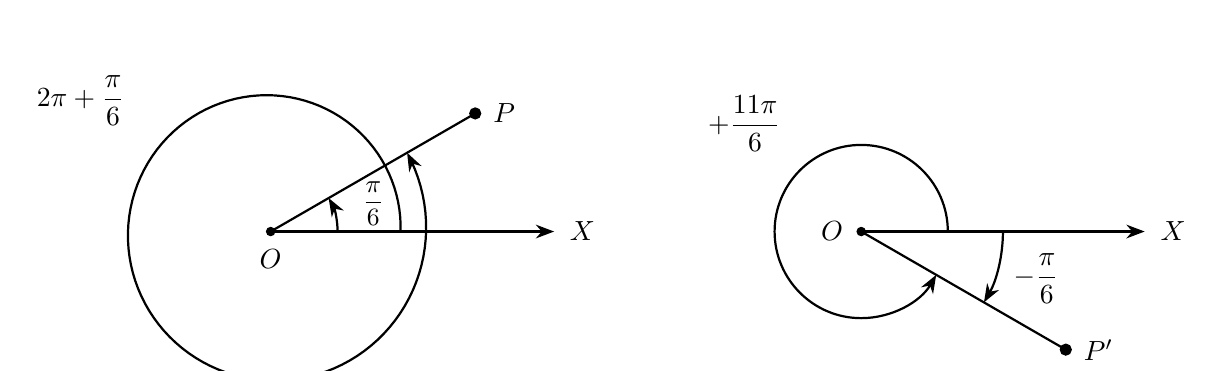
\begin{tikzpicture}[scale=1.0]
  % Left subfigure: P at pi/6 and 2pi + pi/6
  \begin{scope}[shift={(0, 0)}]
    \coordinate (O1) at (0, 0);
    \coordinate (P1) at (30:3.0);

    \draw[thick, -Stealth] (O1) -- (3.6, 0) node[right=2pt] {$X$};
    \draw[thick] (O1) -- (P1);
    \filldraw (O1) circle (1.5pt) node[below=3pt] {$O$};
    \filldraw (P1) circle (2pt) node[right=3pt] {$P$};

    % Inner angle arc pi/6
    \draw[thick, -Stealth] (0.85, 0) arc (0:30:0.85);
    \node at (15:1.35) {\small $\dfrac{\pi}{6}$};

    % Outer spiral arc 2pi + pi/6
    \draw[thick, -Stealth] plot[domain=0:390, samples=120, variable=\t] ({\t}:{1.65 + 0.0009*\t});
    \node[above left=2pt] at (145:2.05) {$2\pi + \dfrac{\pi}{6}$};
  \end{scope}

  % Right subfigure: P' at -pi/6 and +11pi/6
  \begin{scope}[shift={(7.5, 0)}]
    \coordinate (O2) at (0, 0);
    \coordinate (P2) at (-30:3.0);

    \draw[thick, -Stealth] (O2) -- (3.6, 0) node[right=2pt] {$X$};
    \draw[thick] (O2) -- (P2);
    \filldraw (O2) circle (1.5pt) node[left=3pt] {$O$};
    \filldraw (P2) circle (2pt) node[right=3pt] {$P'$};

    % Counterclockwise arc +11pi/6
    \draw[thick, -Stealth] (1.1, 0) arc (0:330:1.1);
    \node[above left=2pt] at (135:1.2) {$+\dfrac{11\pi}{6}$};

    % Clockwise arc -pi/6
    \draw[thick, -Stealth] (1.8, 0) arc (0:-30:1.8);
    \node at (-15:2.3) {$-\dfrac{\pi}{6}$};
  \end{scope}
\end{tikzpicture}
\caption{極座標表法之非唯一性}
\label{fig:b5s-1-3}
\end{figure}

左圖 $\left[2, \dfrac{\pi}{6}\right]$ 與 $\left[2, 2\pi + \dfrac{\pi}{6}\right]$ 都描述同一點 $P$，右圖 $\left[2, -\dfrac{\pi}{6}\right]$ 與 $\left[2, 2\pi - \dfrac{\pi}{6}\right]$ 也都描述同一點 $P'$。

而所有 $[0, \theta]$，$\theta$ 為任何角度，都描述原點 $O$

（更進一步，$\left[-2, \pi + \dfrac{\pi}{6}\right]$ 是否也利於看成 $P$ 點的極座標？）

這些現象雖然顯出極座標先天的一些缺陷，但卻不因此失去它在某些特定問題的處理上（如星體運動的問題）優於直角座標的長處。

現在我們重作說明：

給定平面上一個直角座標系 $(O; X, Y)$，或稱自然座標系 $(O; \mathbf{i}_1, \mathbf{i}_2)$，則對平面上任一點 $P$，有
\[ \vec{OP} = x\mathbf{i}_1 + y\mathbf{i}_2 \]
或記成 $P = (x, y)$

這 $(x, y)$ 稱為 $P$ 的直角座標。

\begin{figure}[H]
\centering
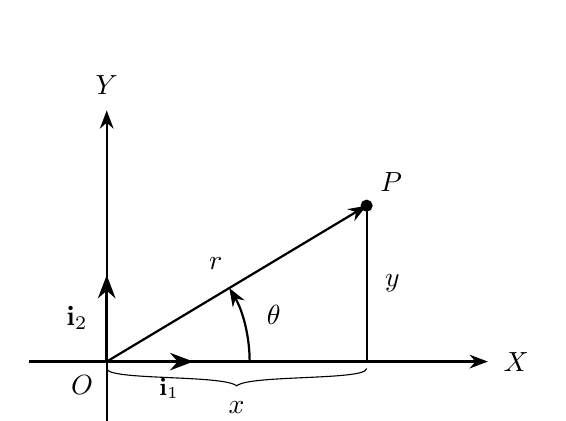
\begin{tikzpicture}[scale=1.1]
  \coordinate (O) at (0, 0);
  \coordinate (P) at (3.0, 1.8);
  \coordinate (Px) at (3.0, 0);

  % Axes
  \draw[thick, -Stealth] (-0.9, 0) -- (4.4, 0) node[right=2pt] {$X$};
  \draw[thick, -Stealth] (0, -0.8) -- (0, 2.9) node[above=2pt] {$Y$};
  \node[below left=2pt] at (O) {$O$};

  % Unit vectors i1, i2
  \draw[very thick, -Stealth] (O) -- (1.0, 0);
  \node[below=2pt] at (0.72, -0.02) {\small $\mathbf{i}_1$};
  \draw[very thick, -Stealth] (O) -- (0, 1.0) node[midway, left=3pt] {$\mathbf{i}_2$};

  % Vector OP and projection
  \draw[thick, -Stealth] (O) -- (P) node[midway, above left=2pt] {$r$};
  \draw[thick] (P) -- (Px) node[midway, right=3pt] {$y$};
  \filldraw (P) circle (1.8pt) node[above right=2pt] {$P$};

  % Angle arc theta
  \draw[thick, -Stealth] (1.65, 0) arc (0:30.96:1.65);
  \node at (15.5:2.0) {$\theta$};

  % Horizontal brace for x
  \draw (0, -0.08) .. controls (0, -0.22) and (1.35, -0.15) .. (1.5, -0.28)
                   .. controls (1.65, -0.15) and (3.0, -0.22) .. (3.0, -0.08);
  \node[below=2pt] at (1.5, -0.28) {$x$};
\end{tikzpicture}
\caption{直角座標與極座標之關係}
\label{fig:b5s-1-4}
\end{figure}

另一方面，取\phantomsection\label{note:b5s-ch1-p4-ge0}
\begin{align*}
r &= \overline{OP} \ge 0\footnotemark && \text{〔稱為向徑〕} \\
\theta &= \vec{OP} \text{ 的矢角} \\
&= \text{自射線 } \vec{OX} \text{ 到 } \vec{OP} \text{ 的轉角角度} && \text{〔稱為幅角〕}
\end{align*}
\footnotetext{【原書註記/校訂】：原書此處不等式右端之「$0$」誤排為英文字母「$O$」（印作「$r = \overline{OP} \ge O$」），茲據下文「$r > 0$」、「$r = 0$」校訂為數字「$0$」。}
其中當 $P$ 不為原點 $O$ 時（卽 $r > 0$ 時）$\theta$ 限制在 $-\pi < \theta \le \pi$ 者稱為\textbf{幅角的主值}或簡稱\textbf{主幅角}。當 $P$ 卽為原點 $O$ 時（卽 $r = 0$ 時），$\theta$ 取為任意角度，這樣的 $[r, \theta]$ 稱為 $P$ 點的極座標，記成 $P = [r, \theta]$，〔註〕。同時，提起 $P$ 點時，為表明其位置，有時記成 $P[r, \theta]$。（$O$ 稱為原點或極，$\vec{OX}$ 稱為極軸）。

〔註〕本書為與直角座標作一區別，特記作 $[r, \theta]$，習慣上亦有記成 $(r, \theta)$ 者。

配置了極座標後的平面，有時為了區別，特稱為\textbf{極平面}。
\paragraph{注意：}
若取 $\theta_0$ 為 $P$ 點幅角的主值，則對任意整數 $n$，$\theta_0 + 2n\pi$ 都是 $P$ 點的幅角。

由三角函數 $\sin\theta, \cos\theta$ 的定義，立刻得到同一點 $P$ 的直角座標與極座標間存在著如下的關係：
\begin{equation}
\begin{cases}
x = r \cos\theta \\
y = r \sin\theta
\end{cases} \label{eq:b5s-1-1-1}
\end{equation}
換句話說
\[ \vec{OP} = r \cos\theta\,\mathbf{i}_1 + r \sin\theta\,\mathbf{i}_2 \]

這個式子給出了已知 $[r, \theta]$ 求 $(x, y)$ 的關係式。反過來如果已知 $P$ 的直角座標 $(x, y)$，想求得 $P$ 的極座標 $[r, \theta]$（換句話說，就是已知 $x, y$，想求得滿足 \eqref{eq:b5s-1-1-1} 式的 $r, \theta$）我們可先將 \eqref{eq:b5s-1-1-1} 中兩式分別平方\phantomsection\label{note:b5s-ch1-p4-pingfang}\footnote{【原書註記/校訂】：原書「平方」二字鉛字磨損漏印，殘存字跡作「个力」，茲據文意與下式校訂補全為「平方」。}後取和得
\[ x^2 + y^2 = r^2(\cos^2\theta + \sin^2\theta) = r^2 \]
再將 \eqref{eq:b5s-1-1-1} 中兩式互除得
\[ \frac{y}{x} = \tan\theta \]
［當 $x = 0$ 時，$\theta$ 之幅角為 $\dfrac{\pi}{2}$ 或 $-\dfrac{\pi}{2}$——依 $y$ 值為正或為負來決定，故不妨假設 $x \ne 0$］

併在一起，寫成：
\begin{equation}
\begin{cases}
r = \sqrt{x^2 + y^2} \\[4pt]
\tan\theta = \dfrac{y}{x}
\end{cases} \label{eq:b5s-1-1-2}
\end{equation}
如此，則描述 $P$ 點之 $[r, \theta]$ 都合於 \eqref{eq:b5s-1-1-2} 式，但是從 \eqref{eq:b5s-1-1-2} 式解出來的 $[r, \theta]$ 並不一定都描述 $P$ 點，也可能解出來的是 $P$ 關於原點 $O$ 的對稱點 $P'$（卽 $\vec{OP'} = -\vec{OP}$）。必須再由 $x$ 或 $y$ 的正負決定 $\theta$ 應取何值方能準確地描出來 $P$ 點。〔注意所取的 $\theta$ 仍非唯一決定，不過限制 $\theta$ 取主幅角時，$\theta$ 便唯一決定了〕

\begin{figure}[H]
\centering
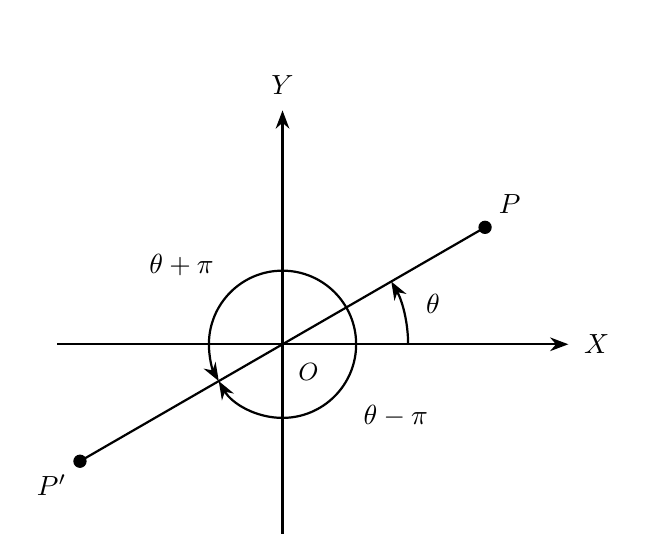
\begin{tikzpicture}[scale=1.1]
  \coordinate (O) at (0, 0);
  \coordinate (P) at (30:2.7);
  \coordinate (Pp) at (210:2.7);

  % Axes
  \draw[thick, -Stealth] (-2.6, 0) -- (3.3, 0) node[right=2pt] {$X$};
  \draw[thick, -Stealth] (0, -2.3) -- (0, 2.7) node[above=2pt] {$Y$};
  \node at (0.3, -0.32) {\small $O$};

  % Line P'OP
  \draw[thick] (Pp) -- (P);
  \filldraw (P) circle (2pt) node[above right=2pt] {$P$};
  \filldraw (Pp) circle (2pt) node[below left=2pt] {$P'$};

  % Angle theta
  \draw[thick, -Stealth] (1.45, 0) arc (0:30:1.45);
  \node at (15:1.8) {$\theta$};

  % Angle theta + pi (upper arc)
  \draw[thick, -Stealth] (0.85, 0) arc (0:210:0.85);
  \node[above left=2pt] at (135:0.9) {$\theta + \pi$};

  % Angle theta - pi (lower arc)
  \draw[thick, -Stealth] (0.85, 0) arc (0:-150:0.85);
  \node[below right=2pt] at (-35:0.95) {$\theta - \pi$};
\end{tikzpicture}
\caption{$\tan\theta = \dfrac{y}{x}$ 之對稱點 $P$ 與 $P'$ 的幅角關係}
\label{fig:b5s-1-5}
\end{figure}

\subsubsection*{作業 1}
\begin{enumerate}[(i)]
  \item 驗證 $[r, \theta]$ 為 $\left[2, \dfrac{\pi}{6}\right]$ 或 $\left[2, \pi + \dfrac{\pi}{6}\right]$ 時都會滿足
  \begin{equation}
  \begin{cases}
  r = \sqrt{\sqrt{3}^2 + 1^2} \\[4pt]
  \tan\theta = \dfrac{1}{\sqrt{3}}
  \end{cases} \tag{$2'$} \label{eq:b5s-1-1-2p}
  \end{equation}
  並描出這兩點 $P = \left[2, \dfrac{\pi}{6}\right]$ 與 $P' = \left[2, \pi + \dfrac{\pi}{6}\right]$ 的位置。
  \item 當某點 $P$ 之直角座標 $(x, y) = (\sqrt{3}, 1)$ 時，由 \eqref{eq:b5s-1-1-2p}，求其極座標 $[r, \theta]$ 中的 $r, \theta$，而 $\theta$ 取主幅角。

  又當 $(x, y) = (-\sqrt{3}, -1)$ 時，$[r, \theta] = ?$
\end{enumerate}

\subsubsection*{作業 2}
驗證 $[r, \theta]$ 為 $\cdots\cdots \left[2, \dfrac{\pi}{6} - 2\pi\right], \left[2, \dfrac{\pi}{6}\right], \left[2, \dfrac{\pi}{6} + 2\pi\right], \left[2, \dfrac{\pi}{6} + 4\pi\right], \cdots\cdots\cdots$ 時，$r, \theta$ 皆滿足 \eqref{eq:b5s-1-1-2p} 式。

問這一系列的實數序對是否描述同一點？試一一描點，並給出它們所相應的直角座標。

\subsubsection*{習題 I-1}
\begin{enumerate}
  \item 設 $[r, \theta]$ 為平面上點的極座標，求其相應的直角座標 $(x, y)$，並描點比較。
  \begin{multicols}{2}
  \begin{enumerate}[(a)]
    \item $\left[2, \dfrac{\pi}{4}\right]$
    \item $\left[3, \dfrac{5\pi}{6}\right]$
    \item $\left[2, \dfrac{13\pi}{4}\right]$
    \item $\left[1, -\dfrac{14\pi}{6}\right]$
    \item $[2.4, -15^\circ]$
    \item $[18, 19^\circ 32']$（查表）
  \end{enumerate}
  \end{multicols}

  \item 設 $(x, y)$ 為平面上點的直角座標，求其相應的極座標 $[r, \theta]$ 並描點比較，其中 $\theta$ 為主幅角。
  \begin{multicols}{2}
  \begin{enumerate}[(a)]
    \item $(-1, -1)$
    \item $(-1, \sqrt{3})$
    \item $(\sqrt{3}, -1)$
    \item $(0, 6.9243)$
    \item $(4.9130, 0.9285)$（查表）
    \item $(1.2, 5.79)$
  \end{enumerate}
  \end{multicols}

  \item 若 $\tan\theta = 0.5658$，而限制 $\theta$ 於 $-\pi < \theta \le \pi$ 時，應有幾個 $\theta$ 滿足上式？當限制 $\theta$ 於 $-\dfrac{\pi}{2} < \theta \le \dfrac{\pi}{2}$ 時，則又如何？是否你的結果可推廣於一般 $\tan\theta = x$ 的情形？〔粗略判斷〕

  \item 求平面上 $P_1[r_1, \theta_1]$ 與 $P_2[r_2, \theta_2]$ 間的距離，分別以
  \begin{enumerate}[(i)]
    \item 變換成直角座標，
    \item 直接利用餘弦定律等方法求出，
  \end{enumerate}
  以 $P_1 = \left[2, \dfrac{\pi}{4}\right], P_2 = \left[1, -\dfrac{14\pi}{6}\right]$ 驗證你的結果（卽將你的式子代以各 $r_i, \theta_i$ 值，結果是否與你將 $\left[2, \dfrac{\pi}{4}\right]$ 與 $\left[1, -\dfrac{14\pi}{6}\right]$ 以你第 1 題所求出的直角座標表達再求距離的結果一致？）。

  \item 若三角形的三頂點為 $[0, 0], [r_1, \theta_1]$ 與 $[r_2, \theta_2]$，則其面積為：
  \[ \frac{1}{2} |r_1 r_2 \sin(\theta_1 - \theta_2)|, \quad \text{試證之。} \]
\end{enumerate}
% =========================================================================
% §I-2 反三角函數 (Pages 7–22)
% =========================================================================
\subsection{反三角函數}\label{sec:b5s-1-2}

第二冊中我們談過反函數，並指明對數函數為指數函數的反函數。至於三角函數的反函數，在上節從直角座標求極座標的過程中：已知 $y/x$，想找滿足
\[
\tan \theta = y/x
\]
的角度 $\theta$ 時，我們看出引入 $\tan$ 的反函數 $\tan^{-1}$ 而將上式換寫成
\[
\theta = \tan^{-1} \frac{y}{x}
\]
將帶來一些\underline{方便}。

但三角函數值相同的角度，經常並非唯一，上節已見其頗為困擾
（如 $\tan \dfrac{\pi}{6} = \tan\left(\pi + \dfrac{\pi}{6}\right) = \tan\left(2\pi + \dfrac{\pi}{6}\right) = \cdots\cdots = \dfrac{1}{\sqrt{3}}$，$\theta$ 應為 $\dfrac{\pi}{6}$，$\pi + \dfrac{\pi}{6}$ 或 $2\pi + \dfrac{\pi}{6}$？）

在下文中，我們首先藉兩個論例\underline{複習反函數的用意及函數圖形}，歸成甲段。然後我們在乙，丙兩段中再回來討論「反三角函數」。

\subsubsection*{甲、反函數的用意與函數圖形}

\begin{discussion}\label{disc:b5s-1-1}
設 $f(x) = 2x + 1$，圖解如下（圖 2-1）知經 $f$ 後「$\cdots\cdots$，$0$ 映射到 $1$，$1$ 映射到 $3$，$2$ 映射到 $5$，$\cdots\cdots\cdots$」，

\begin{center}
\begin{tikzpicture}[>=Stealth, scale=0.85]
  % Left vertical line A = R
  \draw[thick] (0, -3.6) -- (0, 5.6);
  \node[below] at (0, -3.7) {$A = \mathbb{R}$};

  % Right vertical line B = R
  \draw[thick] (4.5, -3.6) -- (4.5, 5.6);
  \node[below] at (4.5, -3.7) {$B = \mathbb{R}$};

  % Dots on A (x = -3 to 5) and B (y = -5 to 7)
  \foreach \x/\y in {-3/-3.0, -2/-2.3, -1/-1.6, 0/-0.9, 1/-0.2, 2/0.5, 3/1.2, 4/1.9, 5/2.6} {
    \fill (0, \y) circle (2pt);
    \node[left=3pt, font=\small] at (0, \y) {$\x$};
  }
  \foreach \val/\yb in {-5/-3.4, -3/-2.5, -1/-1.6, 1/-0.7, 3/0.2, 5/1.1, 7/2.0} {
    \fill (4.5, \yb) circle (2pt);
    \node[right=3pt, font=\small] at (4.5, \yb) {$\val$};
  }

  % Mapping arrows for x = -3..3 to y = -5..7
  \foreach \ya/\yb in {-3.0/-3.4, -2.3/-2.5, -1.6/-1.6, -0.9/-0.7, -0.2/0.2, 0.5/1.1, 1.2/2.0} {
    \draw[->, semithick] (0.12, \ya+0.05) -- (4.38, \yb+0.05);
    \draw[<-, dashed, semithick] (0.12, \ya-0.06) -- (4.38, \yb-0.06);
  }

  % Partial arrows for 4 -> 9 and 5 -> 11
  \draw[->, semithick] (0.12, 1.9+0.05) -- (3.3, 2.75);
  \draw[<-, dashed, semithick] (0.12, 1.9-0.06) -- (3.3, 2.64);
  \node[right=1pt, font=\small] at (3.3, 2.72) {$9$};

  \draw[->, semithick] (0.12, 2.6+0.05) -- (1.6, 3.05);
  \draw[<-, dashed, semithick] (0.12, 2.6-0.06) -- (1.6, 2.94);
  \node[right=1pt, font=\small] at (1.6, 3.02) {$11$};

  % Legend arrows at bottom
  \draw[->, thick] (1.5, -4.0) -- (3.0, -4.0);
  \node[below=1pt] at (2.25, -4.0) {$f$};
  \draw[<-, dashed, thick] (1.5, -4.7) -- (3.0, -4.7);
  \node[below=1pt] at (2.25, -4.7) {$f^{-1}$};

  \node[below] at (2.25, -5.5) {\textbf{圖 2-1}};
\end{tikzpicture}
\end{center}

\noindent 或寫成「$\cdots\cdots$，$f(0)=1$，$f(1)=3$，$f(2)=5$，$\cdots\cdots$」。

\underline{引入反函數 $f^{-1}$} 的意思就是要把「$\cdots\cdots 1$ 映回來 $0$，$3$ 映回來 $1$，$5$ 映回來 $2$，$\cdots\cdots$」寫成
「$\cdots\cdots$，$f^{-1}(1)=0$，$f^{-1}(3)=1$，$f^{-1}(5)=2$，$\cdots\cdots$」，此時 $0$ 經 $f$ 到 $1$ 後經 $f^{-1}$ 又回來 $0$。另一方面，$1$ 經 $f^{-1}$ 來到 $0$ 後經 $f$ 又回去 $1$，書寫如下式
\[
\begin{cases}
f^{-1} f(0) = f^{-1}(1) = 0 \\[0.3em]
f f^{-1}(1) = f(0) = 1
\end{cases}
\quad\text{〔註〕}\footnotemark
\]
\phantomsection\label{note:b5s-ch1-invdef}\footnotetext{【原書註記】：這式子一般化後便成為反函數的定義：$f : X \longrightarrow Y$，設另一個函數 $g : Y \longrightarrow X$，若滿足 $\begin{cases} g \circ f(a) = a, & \forall a \in X \\ f \circ g(b) = b, & \forall b \in Y \end{cases}$ 其中 $g \circ f$ 表先 $f$ 後 $g$ 的合成函數，則稱 $g$ 為 $f$ 之反函數，又因對於 $f$，這樣的 $g$ 是唯一的，記 $g$ 為 $f^{-1}$。}

這時候\underline{方便}上，我們說「$0$ 與 $1$ 對射」記成 $0 \longleftrightarrow 1$，同樣也有 $1 \longleftrightarrow 3$，$2 \longleftrightarrow 5$，$\cdots\cdots$等等。

用函數圖形來表達，$f : y = 2x + 1$ 表示直角座標 $(x, y)$ 平面上，斜率為 $2$，$Y$ 軸上截距為 $1$ 的直線，這直線含下列各點：
\[
\text{「}\cdots\cdots,\ (0, 1),\ (1, 3),\ (2, 5),\ \cdots\cdots\text{」}
\]

\begin{center}
\begin{tikzpicture}[>=Stealth, scale=0.68]
  % Axes
  \draw[->, thick] (-2.2, 0) -- (4.8, 0) node[right] {$X$};
  \draw[->, thick] (0, -2.0) -- (0, 6.8) node[left] {$Y$};
  \node[below right=1pt, font=\small] at (0, 0) {$O$};

  % Ticks on Y axis
  \foreach \y in {1, 3, 5} {
    \draw (-0.1, \y) -- (0.1, \y);
    \node[left=2pt, font=\small] at (-0.05, \y) {$\y$};
  }

  % Line y = 2x + 1 from x = -1.2 to x = 2.4
  \draw[thick] (-1.2, -1.4) -- (2.4, 5.8);

  % Points
  \fill (-1, -1) circle (2.2pt);
  \node[right=3pt, fill=white, inner sep=1pt, font=\small] at (-0.98, -1.0) {$(-1, -1)$};

  \fill (0, 1) circle (2.2pt);
  \node[right=3pt, font=\small] at (0, 0.95) {$(0, 1)$};

  \fill (1, 3) circle (2.2pt);
  \node[right=3pt, font=\small] at (1, 3) {$(1, 3)$};

  \fill (2, 5) circle (2.2pt);
  \node[right=3pt, font=\small] at (2, 5) {$(2, 5)$};

  \node[above right=1pt, font=\small] at (2.4, 6.0) {$(3, 7)$};

  \node[below] at (2.0, -2.2) {\textbf{圖 2-2}};
\end{tikzpicture}
\end{center}

注意：這些點的橫、縱座標正是上述 $\mathbb{R}$ 上經 $f$ 互為對射的數對；
\[
\text{「}\cdots\cdots,\ 0 \longleftrightarrow 1,\ 1 \longleftrightarrow 3,\ 2 \longleftrightarrow 5,\ \cdots\cdots\text{」}
\]

現在，如果我們把 $Y$ 軸看成 $f^{-1}$ 的定義的地方，$X$ 軸看成 $f^{-1}$ 取值的地方，上圖中（圖 2-2），原來直線實際上便已是 $f^{-1}$ 的函數圖形，例如
\begin{align*}
y = 1 \text{ 時} &\longrightarrow f^{-1}(y) = x = 0 \\
y = 3 \text{ 時} &\longrightarrow f^{-1}(y) = x = 1 \\
y = 5 \text{ 時} &\longrightarrow f^{-1}(y) = x = 2
\end{align*}
但這樣反過來以 $Y$ 軸為\underline{定義}的地方，$X$ 軸為\underline{取值}的地方，所得的函數圖形不太適合我們的習慣，我們將它翻轉如下：（圖 2-3）

\begin{center}
\begin{tikzpicture}[>=Stealth, scale=0.78]
  % --- Panel (a) ---
  \begin{scope}[xshift=0cm]
    \draw[thick] (0, 0) rectangle (2.8, 3.2);
    \draw[->, semithick] (0.2, 0.7) -- (2.6, 0.7) node[below left=1pt, font=\footnotesize] {$X$};
    \draw[->, semithick] (0.7, 0.2) -- (0.7, 3.0) node[below left=1pt, font=\footnotesize] {$Y$};
    \draw[thick] (0.2, 0.2) -- (1.7, 3.0);
    \node[below left, font=\footnotesize] at (2.8, 0) {正面};
    \node[below] at (1.4, -0.5) {\textbf{圖 2-3(a)}};
  \end{scope}

  \draw[->, thick] (2.95, 1.6) -- (3.65, 1.6);

  % --- Panel (b) ---
  \begin{scope}[xshift=3.8cm]
    \draw[thick] (0, 0) -- (1.3, 0) -- (1.3, 3.2) -- (0, 3.2) -- cycle;
    % Turning page flap
    \draw[thick, fill=white] (1.3, 0) .. controls (1.7, 0.2) and (1.9, 0.5) .. (2.0, 0.8)
      -- (2.0, 3.2) .. controls (1.8, 3.0) and (1.5, 2.9) .. (1.3, 3.2) -- cycle;
    \draw[->, semithick] (0.2, 0.7) -- (1.25, 0.7);
    \draw[->, semithick] (0.7, 0.2) -- (0.7, 3.0) node[below left=1pt, font=\footnotesize] {$Y$};
    \draw[thick] (0.2, 0.2) -- (1.25, 2.15);
    \draw[->, semithick] (1.95, 0.15) to[bend left=25] (1.45, -0.15);
    \node[right, font=\footnotesize] at (1.9, -0.05) {翻面};
    \node[below] at (1.1, -0.5) {\textbf{圖 2-3(b)}};
  \end{scope}

  \draw[->, thick] (6.1, 1.6) -- (6.8, 1.6);

  % --- Panel (c) ---
  \begin{scope}[xshift=7.0cm]
    \draw[thick] (0, 0) rectangle (2.8, 3.2);
    \draw[->, semithick] (2.6, 0.7) -- (0.2, 0.7) node[below right=1pt, font=\footnotesize] {$X$};
    \draw[->, semithick] (2.1, 0.2) -- (2.1, 3.0) node[below right=1pt, font=\footnotesize] {$Y$};
    \draw[thick] (2.6, 0.2) -- (1.1, 3.0);
    % 90 degree rotation arrow at top right
    \draw[->, semithick] (2.95, 3.0) arc (-10:100:0.35);
    \node[above right, font=\footnotesize] at (2.95, 3.1) {$90^\circ$};
    \node[below left, font=\footnotesize] at (2.8, 0) {背面};
    \node[below] at (1.4, -0.5) {\textbf{圖 2-3(c)}};
  \end{scope}

  \draw[->, thick] (10.0, 1.6) -- (10.7, 1.6);

  % --- Panel (d) ---
  \begin{scope}[xshift=10.9cm]
    \draw[thick] (0, 0) rectangle (2.8, 3.2);
    \draw[->, semithick] (0.2, 0.7) -- (2.6, 0.7) node[below left=1pt, font=\footnotesize] {$Y$};
    \draw[->, semithick] (0.7, 0.2) -- (0.7, 3.0) node[below left=1pt, font=\footnotesize] {$X$};
    \draw[thick] (0.2, 0.35) -- (2.6, 1.65);
    \node[below left, font=\footnotesize] at (2.8, 0) {背面};
    \node[below] at (1.4, -0.5) {\textbf{圖 2-3(d)}};
  \end{scope}
\end{tikzpicture}
\end{center}

\vspace{0.3em}
\begin{center}
\begin{tikzpicture}[>=Stealth, scale=0.85]
  \node[left] at (-1.8, 2.2) {（改記 $Y$ 為 $X$，$X$ 為 $Y$）};

  % Axes
  \draw[->, thick] (-1.5, 0) -- (4.8, 0) node[below left] {$X$};
  \draw[->, thick] (0, -1.3) -- (0, 4.2) node[below right] {$Y$};

  % Mirror axis x = y
  \draw[dashed, semithick] (-1.1, -1.1) -- (3.6, 3.6);
  \node[above left=1pt] at (2.3, 2.3) {$x = y$};

  % Line f: y = 2x + 1
  \draw[thick] (-0.95, -0.9) -- (1.5, 4.0);
  \draw[->, semithick] (1.35, 3.65) .. controls (1.15, 3.65) and (1.1, 3.45) .. (0.95, 3.45);
  \node[right=1pt] at (1.35, 3.7) {$f$};

  % Line f^{-1}: y = 0.5x - 0.5
  \draw[thick] (-1.1, -1.05) -- (4.2, 1.6);
  \draw[->, semithick] (4.1, 1.75) .. controls (3.9, 1.75) and (3.9, 1.5) .. (3.75, 1.4);
  \node[above right=1pt] at (4.05, 1.65) {$f^{-1}$};

  \node[below] at (1.6, -1.5) {\textbf{圖 2-3 (e)}};
\end{tikzpicture}
\end{center}

同時我們注意到經過這樣一翻一轉後所得 $f^{-1}$ 的圖形與 $f$ 的圖形正好對稱於鏡射軸 $x = y$。

$f^{-1}$ 表示式可求之如下：
\[
f : y = 2x + 1
\]
解 $x$ 得
\[
x = \frac{y}{2} - \frac{1}{2}
\]
為沿依習慣，將自變數 $y$ 改記為 $x$，應變數 $x$ 改記為 $y$，得
\[
f^{-1} : y = \frac{x}{2} - \frac{1}{2}
\]
描圖果然與上文所說「$f$ 與 $f^{-1}$ 的圖形對稱於 $x = y$ 軸」一事相符。
\end{discussion}

\begin{discussion}\label{disc:b5s-1-2}
\begin{align*}
f &: y = 2^x, \\
f^{-1} &: y = \log_2 x,
\end{align*}
互為反函數，仿論例 1，得映射圖如下（圖 2-4）其中 $A \equiv \mathbb{R}$ 與 $B \equiv (0, \infty)$ 間存在一對射。

如
\begin{align*}
-1 &\longleftrightarrow 0.5, & 0 &\longleftrightarrow 1 \\
1 &\longleftrightarrow 2, & 2 &\longleftrightarrow 4
\end{align*}

\begin{center}
\begin{tikzpicture}[>=Stealth, scale=0.88]
  % Left vertical line A = R
  \draw[thick] (0, -2.8) -- (0, 3.0);
  \node[below] at (0, -2.9) {$A \equiv \mathbb{R}$};

  % Right vertical ray B = (0, \infty)
  \draw[thick] (4.5, -0.1) -- (4.5, 4.5);
  \draw[thick, fill=white] (4.5, -0.1) circle (2.2pt);
  \node[right=4pt, font=\small] at (4.5, -0.15) {$0$};
  \node[below] at (4.5, -0.9) {$B \equiv (0, \infty)$};

  % Points on A: -2, -1, 0, 0.5, 1, 2
  \foreach \x/\ya in {-2/-2.2, -1/-1.1, 0/0.0, 0.5/0.6, 1/1.2, 2/2.2} {
    \fill (0, \ya) circle (2pt);
    \node[left=3pt, font=\small] at (0, \ya) {$\x$};
  }

  % Points on B: 0.25, 0.5, 1, 1.414, 2, 4 (well-spaced vertically)
  \fill (4.5, 0.4) circle (2pt);
  \node[right=4pt, font=\small] at (4.5, 0.4) {$0.25$};

  \fill (4.5, 0.9) circle (2pt);
  \node[right=4pt, font=\small] at (4.5, 0.9) {$0.5$};

  \fill (4.5, 1.45) circle (2pt);
  \node[right=4pt, font=\small] at (4.5, 1.45) {$1$};

  \fill (4.5, 2.0) circle (2pt);
  \node[right=4pt, font=\small] at (4.5, 2.0) {$1.414$};

  \fill (4.5, 2.65) circle (2pt);
  \node[right=4pt, font=\small] at (4.5, 2.65) {$2$};

  \fill (4.5, 4.1) circle (2pt);
  \node[right=4pt, font=\small] at (4.5, 4.1) {$4$};

  % Paired arrows between A and B
  \foreach \ya/\yb in {-2.2/0.4, -1.1/0.9, 0.0/1.45, 0.6/2.0, 1.2/2.65, 2.2/4.1} {
    \draw[->, semithick] (0.12, \ya+0.05) -- (4.38, \yb+0.05);
    \draw[<-, semithick] (0.12, \ya-0.05) -- (4.38, \yb-0.05);
  }

  % Legend arrows
  \draw[->, thick] (1.6, -2.0) -- (3.0, -2.0);
  \node[above=1pt] at (2.3, -2.0) {$f$};
  \draw[<-, thick] (1.6, -2.35) -- (3.0, -2.35);
  \node[below=1pt] at (2.3, -2.35) {$f^{-1}$};

  \node[below] at (2.3, -3.4) {\textbf{圖 2-4}};
\end{tikzpicture}
\end{center}

同時亦得 $f$ 與 $f^{-1}$ 之函數圖形（圖 2-5）如下

\begin{center}
\begin{tikzpicture}[>=Stealth, scale=0.92]
  % Axes
  \draw[->, thick] (-1.8, 0) -- (5.2, 0) node[right] {$X$};
  \draw[->, thick] (0, -1.6) -- (0, 4.8) node[left] {$Y$};

  % Ticks
  \foreach \x in {1, 2, 3, 4} {
    \draw (\x, -0.08) -- (\x, 0.08);
  }
  \foreach \y in {1, 2, 3, 4} {
    \draw (-0.08, \y) -- (0.08, \y);
  }

  % Symmetry line y = x
  \draw[semithick] (-1.2, -1.2) -- (4.0, 4.0);

  % Curve f(x) = 2^x
  \draw[very thick, domain=-1.3:2.15, samples=80] plot (\x, {pow(2, \x)});
  \node[right] at (2.2, 4.35) {$f(x) = 2^x$};
  \draw[->, semithick] (2.25, 4.3) .. controls (2.05, 4.3) and (2.05, 4.1) .. (1.9, 4.05);

  % Points on f(x) = 2^x
  \fill (-1, 0.5) circle (2pt);
  \node[above left=2pt, font=\small] at (-1, 0.5) {$(-1, 0.5)$};

  \fill (0, 1) circle (2pt);
  \node[above left=2pt, font=\small] at (0, 1.05) {$(0, 1)$};

  \fill (1, 2) circle (2pt);
  \node[right=1.5pt, fill=white, inner sep=0.8pt, font=\footnotesize] at (1.03, 1.98) {$(1, 2)$};

  \fill (2, 4) circle (2pt);
  \node[left=3pt, font=\small] at (2, 4.0) {$(2, 4)$};

  % Curve f^{-1}(x) = \log_2 x (plotted parametrically as (2^t, t))
  \draw[very thick, domain=-1.3:2.15, samples=80] plot ({pow(2, \x)}, \x);
  \node[right] at (4.1, 2.3) {$f^{-1}(x) = \log_2 x$};
  \draw[->, semithick] (4.15, 2.25) .. controls (3.95, 2.25) and (3.95, 2.05) .. (3.8, 2.0);

  % Points on f^{-1}(x) = \log_2 x
  \fill (0.5, -1) circle (2pt);
  \node[right=3pt, font=\small] at (0.5, -1.05) {$(0.5, -1)$};

  \fill (1, 0) circle (2pt);
  \node[below right=2pt, font=\small] at (1.05, -0.02) {$(1, 0)$};

  \fill (2, 1) circle (2pt);
  \node[below right=2pt, font=\small] at (2.0, 1.0) {$(2, 1)$};

  \fill (4, 2) circle (2pt);
  \node[below=3pt, font=\small] at (4.0, 1.95) {$(4, 2)$};

  \node[below] at (2.0, -1.8) {\textbf{圖 2-5}};
\end{tikzpicture}
\end{center}
\end{discussion}

這一論例已告訴我們，雖然 $f(x) = 2^x$ 不是 $\mathbb{R} \longrightarrow \mathbb{R}$ 的蓋射，但我們可取 $f$ 的像集 $f(\mathbb{R}) = \{f(x) \mid x \in \mathbb{R}\} = (0, \infty)$ 記之為 $B$，而讓 $f^{-1}$ 只定義在 $B$ 上，即
\[
f^{-1} : \mathbb{R} \longleftarrow B
\]

\textbf{經過這樣的調整，我們知道 $f$ 是不是蓋射，不致於造成要定義 $f^{-1}$ 的不可克服的困難。當然要注意到這時 $f^{-1}$ 所定義的範圍是須要縮小在 $f$ 的像集 $f(\mathbb{R})$ 上。}

下一段我們要進一步看看，\textbf{當 $f$ 甚至連嵌射都不是時，是不是在某些狀況下（如 $f$ 為三角函數的情形），仍可能適當地定義 $f^{-1}$？}

\medskip
\subsubsection*{作業 3}
\begin{enumerate}[label=(\roman*), topsep=2pt, itemsep=2pt]
  \item 問 $f(x) = x^3$ 有否反函數？試仿上文描點，畫其映射圖解。
  \item 又討論 $f(x) = x^2$ 的情形。
\end{enumerate}

\subsubsection*{乙、正弦函數的反函數：$\sin^{-1}$；$\operatorname{Sin}^{-1}$}

給了
\[
f(x) = \sin x
\]
我們先作映射圖解如圖 2-6：

\begin{center}
\begin{tikzpicture}[>=Stealth, xscale=0.88, yscale=1.08]
  % Left line A = R
  \draw[thick] (0, -1.2) -- (0, 3.8);
  \node[below] at (0, -1.35) {$A = \mathbb{R}$};

  % Right segment B = [-1, 1]
  \draw[thick] (4.8, -0.8) -- (4.8, 2.5);
  \node[below] at (4.8, -1.35) {$B = [-1, 1]$};

  % Points on A: 0, \pi/3, \pi/2, 2\pi/3
  \fill (0, 0) circle (2pt);
  \node[left=3pt, font=\small] at (0, 0) {$0$};

  \fill (0, 1.2) circle (2pt);
  \node[left=3pt, font=\small] at (0, 1.2) {$\dfrac{\pi}{3}$};

  \fill (0, 2.15) circle (2pt);
  \node[left=3pt, font=\small] at (0, 2.15) {$\dfrac{\pi}{2}$};

  \fill (0, 3.1) circle (2pt);
  \node[left=3pt, font=\small] at (0, 3.1) {$\dfrac{2\pi}{3}$};

  % Points on B: 0, \sqrt{3}/2, +1
  \fill (4.8, 0) circle (2pt);
  \node[right=3pt, font=\small] at (4.8, 0) {$0$};

  \fill (4.8, 1.0) circle (2pt);
  \node[right=3pt, font=\small] at (4.8, 0.9) {$\dfrac{\sqrt{3}}{2}$};

  \fill (4.8, 1.75) circle (2pt);
  \node[right=3pt, font=\small] at (4.8, 1.78) {$+1$};

  % Mapping arrows
  \draw[->, semithick] (0.12, 0) -- (4.65, 0);
  \draw[->, semithick] (0.12, 1.2) -- (4.65, 0.98);
  \draw[->, semithick] (0.12, 2.15) -- (4.65, 1.75);
  \draw[->, semithick] (0.12, 3.1) -- (4.65, 1.06);

  % Bottom f arrow
  \draw[->, semithick] (2.0, -1.55) -- (2.8, -1.55);
  \node[above=1pt] at (2.4, -1.55) {$f$};

  \node[below] at (2.4, -1.9) {\textbf{圖 2-6}};
\end{tikzpicture}
\end{center}

$\sin x$ 顯然不是嵌射，例如：
\[
\left.
\begin{array}{c}
\dfrac{2\pi}{3} \\[0.6em]
\dfrac{\pi}{3}
\end{array}
\right\} \longrightarrow \frac{\sqrt{3}}{2}
\]
亦即
\[
\sin \frac{\pi}{3} = \frac{\sqrt{3}}{2} = \sin \frac{2\pi}{3}
\]

如果我們要定義 $f^{-1}$，則 $\dfrac{\sqrt{3}}{2}$ 之 $f^{-1}$ 值應取 $\dfrac{\pi}{3}$ 或 $\dfrac{2\pi}{3}$？實際上，不止是 $\dfrac{\pi}{3}$ 與 $\dfrac{2\pi}{3}$ 這兩個值經 $f$ 映射到 $\dfrac{\sqrt{3}}{2}$，所有 $\dfrac{\pi}{3} + 2n\pi$ 與 $\dfrac{2\pi}{3} + 2n\pi$（$n$ 為任意整數），都經 $f$ 映射到 $\dfrac{\sqrt{3}}{2}$，換句話說，在單位圓上設一質點 $P$，自 $(1, 0)$ 依圓周繞行（不限為一圈），只要 $\vec{OP}$ 在 $Y$ 軸上的投影量為 $+\dfrac{\sqrt{3}}{2}$（亦即圖 2-7 中 $P = P_1$，或 $P = P_2$）時，$\vec{OP}$ 的矢角 $\theta$ 都滿足
\[
\sin \theta = \frac{\sqrt{3}}{2}
\]

\begin{center}
\begin{tikzpicture}[>=Stealth, scale=1.4]
  % Axes
  \draw[->, thick] (-1.45, 0) -- (1.6, 0);
  \draw[thick] (0, -1.35) -- (0, 1.45);
  \node[below left=1pt, font=\small] at (0, 0) {$O$};

  % Unit circle
  \draw[thick] (0, 0) circle (1cm);
  \node[below right=1pt, font=\small] at (1, 0) {$(1, 0)$};

  % P1 at 60 deg, P2 at 120 deg
  \draw[thick] (0, 0) -- (60:1) node[above right=1pt, font=\small] {$P_1$};
  \draw[thick] (0, 0) -- (120:1) node[above left=1pt, font=\small] {$P_2$};
  \fill (60:1) circle (1.5pt);
  \fill (120:1) circle (1.5pt);

  % Angle arc for \pi/3
  \draw[->, semithick] (0.3, 0) arc (0:60:0.3);
  \node[font=\footnotesize] at (30:0.52) {$\dfrac{\pi}{3}$};

  \node[below] at (0, -1.45) {\textbf{圖 2-7}};
\end{tikzpicture}
\end{center}

從這裏我們易將
\[
\theta = \frac{\pi}{3} + 2n\pi \quad\text{與}\quad \theta = \frac{2\pi}{3} + 2n\pi \qquad \text{（$n$ 為任意整數）}
\]
的全體整理成\underline{通式}：
\[
\theta = n\pi + (-1)^n \frac{\pi}{3} \qquad \text{（$n$ 為任意整數）}
\]
而稱它們為 $\sin^{-1} \dfrac{\sqrt{3}}{2}$ 的通值。

對這麼多的 $\theta$，取哪一個值來當 $\sin^{-1} \dfrac{\sqrt{3}}{2}$？

現在採用甲段所說將原來 $f : y = \sin x$ 的函數圖形（圖 2-8a）

\begin{center}
\begin{tikzpicture}[>=Stealth, xscale=0.72, yscale=1.05]
  % Axes
  \draw[->, thick] (-7.2, 0) -- (10.6, 0) node[below] {$X$};
  \draw[->, thick] (0, -1.6) -- (0, 1.9) node[right] {$Y$};
  \node[below right=2pt, font=\small] at (0, 0) {$O$};

  % Sine wave y = sin(x)
  \draw[very thick, domain=-6.7:9.8, samples=160] plot (\x, {sin(\x r)});

  % Mark \sqrt{3}/2 on Y-axis
  \fill (0, 0.866) circle (2.2pt);
  \node[left=2pt, font=\footnotesize] at (0, 0.866) {$\dfrac{\sqrt{3}}{2}$};

  % Vertical segments at x where sin(x) = \sqrt{3}/2
  % -2\pi + \pi/3 = -5.236
  \draw[semithick] (-5.236, 0) -- (-5.236, 0.866);
  \fill (-5.236, 0.866) circle (2pt);
  \node[below=4pt, fill=white, inner sep=1pt, font=\scriptsize] at (-5.65, -0.05) {$-2\pi+\dfrac{\pi}{3}$};

  % -\pi - \pi/3 = -4.189
  \draw[semithick] (-4.189, 0) -- (-4.189, 0.866);
  \fill (-4.189, 0.866) circle (2pt);
  \node[below=2pt, font=\scriptsize] at (-3.7, 0) {$-\pi-\dfrac{\pi}{3}$};

  % \pi/3 = 1.047
  \draw[semithick] (1.047, 0) -- (1.047, 0.866);
  \fill (1.047, 0.866) circle (2pt);
  \node[below=2pt, font=\scriptsize] at (1.047, 0) {$\dfrac{\pi}{3}$};

  % \pi - \pi/3 = 2.094
  \draw[semithick] (2.094, 0) -- (2.094, 0.866);
  \fill (2.094, 0.866) circle (2pt);
  \node[below=2pt, font=\scriptsize] at (2.3, 0) {$\pi-\dfrac{\pi}{3}$};

  % 2\pi + \pi/3 = 7.330
  \draw[semithick] (7.330, 0) -- (7.330, 0.866);
  \fill (7.330, 0.866) circle (2pt);
  \node[below=2pt, font=\scriptsize] at (6.85, 0) {$2\pi+\dfrac{\pi}{3}$};

  % 3\pi - \pi/3 = 8.378
  \draw[semithick] (8.378, 0) -- (8.378, 0.866);
  \fill (8.378, 0.866) circle (2pt);
  \node[below=2pt, font=\scriptsize] at (8.85, 0) {$3\pi-\dfrac{\pi}{3}$};

  \node[below] at (1.8, -1.4) {\textbf{圖 2-8 a}};
\end{tikzpicture}
\end{center}

經一翻一轉而得 $f^{-1}$ 的方法，得圖形如下（圖 2-8b）。

圖 2-8b 顯示下列中
\[
\cdots\cdots,\ -2\pi + \frac{\pi}{3},\ -\pi - \frac{\pi}{3},\ 0 + \frac{\pi}{3},\ \pi - \frac{\pi}{3},\ 2\pi + \frac{\pi}{3},\ 3\pi - \frac{\pi}{3},\ \cdots\cdots\cdots
\]
每一個值\underline{都可以}當 $\sin^{-1} \dfrac{\sqrt{3}}{2}$，但這樣 $\sin^{-1}$ 就不符合我們原先對函數所下的定義〔對每一個定義域的元素，都取唯一的確定的值〕了。

於是我們一開始\underline{人為地}取定圖 2-8b 單調遞增或下降的一段曲線，例如 $A_1$ 到 $A_2$ 或 $A_2$ 到 $A_3$ 等，作為 $\sin^{-1}[-1, 1]$ 間的函數圖形。

\begin{center}
\begin{tikzpicture}[>=Stealth, xscale=1.2, yscale=0.68]
  % Axes
  \draw[->, thick] (-2.2, 0) -- (2.3, 0) node[below] {$X$};
  \draw[->, thick] (0, -6.5) -- (0, 9.8) node[right] {$Y$};
  \node[below right=2pt, font=\small] at (0, 0) {$O$};

  % Vertical sine wave x = sin(y)
  \draw[very thick, domain=-6.0:9.0, samples=160] plot ({sin(\x r)}, \x);

  % Extrema points A0, A1, A2, A3, A4
  \fill (1, -4.712) circle (2.2pt);
  \node[right=3pt, font=\small] at (1, -4.712) {$A_0$};

  \fill (-1, -1.571) circle (2.2pt);
  \node[left=3pt, font=\small] at (-1, -1.571) {$A_1$};

  \fill (1, 1.571) circle (2.2pt);
  \node[right=3pt, font=\small] at (1, 1.571) {$A_2$};

  \fill (-1, 4.712) circle (2.2pt);
  \node[left=3pt, font=\small] at (-1, 4.712) {$A_3$};

  \fill (1, 7.854) circle (2.2pt);
  \node[right=3pt, font=\small] at (1, 7.854) {$A_4$};

  % Mark \sqrt{3}/2 on X-axis
  \node[below=2pt, font=\scriptsize] at (0.866, 0) {$\dfrac{\sqrt{3}}{2}$};

  % Horizontal segments at y where sin(y) = \sqrt{3}/2
  % -2\pi + \pi/3 = -5.236
  \draw[semithick] (0, -5.236) -- (0.866, -5.236);
  \fill (0.866, -5.236) circle (2pt);
  \node[left=2pt, font=\scriptsize] at (0, -5.45) {$-2\pi+\dfrac{\pi}{3}$};

  % -\pi - \pi/3 = -4.189
  \draw[semithick] (0, -4.189) -- (0.866, -4.189);
  \fill (0.866, -4.189) circle (2pt);
  \node[left=2pt, font=\scriptsize] at (0, -3.95) {$-\pi-\dfrac{\pi}{3}$};

  % \pi/3 = 1.047
  \draw[semithick] (0, 1.047) -- (0.866, 1.047);
  \fill (0.866, 1.047) circle (2pt);
  \node[left=2pt, font=\scriptsize] at (0, 0.90) {$\dfrac{\pi}{3}$};

  % \pi - \pi/3 = 2.094
  \draw[semithick] (0, 2.094) -- (0.866, 2.094);
  \fill (0.866, 2.094) circle (2pt);
  \node[left=2pt, font=\scriptsize] at (0, 2.25) {$\pi-\dfrac{\pi}{3}$};

  % 2\pi + \pi/3 = 7.330
  \draw[semithick] (0, 7.330) -- (0.866, 7.330);
  \fill (0.866, 7.330) circle (2pt);
  \node[left=2pt, font=\scriptsize] at (0, 7.10) {$2\pi+\dfrac{\pi}{3}$};

  % 3\pi - \pi/3 = 8.378
  \draw[semithick] (0, 8.378) -- (0.866, 8.378);
  \fill (0.866, 8.378) circle (2pt);
  \node[left=2pt, font=\scriptsize] at (0, 8.60) {$3\pi-\dfrac{\pi}{3}$};

  \node[below] at (0, -6.9) {\textbf{圖 2-8 b}};
\end{tikzpicture}
\end{center}

這樣的取法\underline{有一點基本精神}就是要讓所取的 $\sin^{-1}$ 值\underline{連續變化}。例如根據圖 2-9a，$\sin^{-1} \dfrac{\sqrt{3}}{2}$ 取為 $\dfrac{\pi}{3}$，則 $\sin^{-1} \dfrac{1}{\sqrt{2}}$ 取值為 $\dfrac{\pi}{4}$，$\sin^{-1} \dfrac{1}{2}$ 取值為 $\dfrac{\pi}{6}$，其值沿 $A_1 A_2$ 曲線連續變化，而不讓下一情形發生：

「$\sin^{-1} \dfrac{\sqrt{3}}{2}$ 取為 $\dfrac{\pi}{3}$ 在 $A_1 A_2$ 曲線之間，$\sin^{-1} \dfrac{1}{\sqrt{2}}$ 卻又跳到 $A_2 A_3$ 曲線上而取 $\dfrac{3\pi}{4}$ 之值$\cdots\cdots$」如圖 2-9c 所示。

\begin{center}
\begin{tikzpicture}[>=Stealth, scale=1.25]
  % --- 圖 2-9 a ---
  \begin{scope}[xshift=0cm]
    \draw[->, thick] (-1.8, 0) -- (2.3, 0) node[right] {$X$};
    \draw[->, thick] (0, -2.0) -- (0, 2.3) node[right] {$Y$};
    \node[below left=2pt, font=\footnotesize] at (0, 0) {$O$};

    % Curve A1 to A2: x = sin(y)*1.3, y in [-pi/2, pi/2]
    \draw[very thick, domain=-1.571:1.571, samples=80] plot ({sin(\x r)*1.3}, \x);

    % Endpoints A1(-1.3, -pi/2) and A2(1.3, pi/2)
    \fill (-1.3, -1.571) circle (1.8pt);
    \node[below left=1pt, font=\small] at (-1.3, -1.571) {$A_1$};
    \draw[semithick] (-1.3, 0) -- (-1.3, -1.571) -- (0, -1.571);
    \node[above=2pt, font=\footnotesize] at (-1.3, 0) {$-1$};
    \node[right=2pt, font=\scriptsize] at (0, -1.571) {$-\dfrac{\pi}{2}$};

    \fill (1.3, 1.571) circle (1.8pt);
    \node[above=2pt, font=\small] at (1.3, 1.571) {$A_2$};

    % Projections for 1/2 -> pi/6, 1/sqrt{2} -> pi/4, sqrt{3}/2 -> pi/3, 1 -> pi/2
    \draw[semithick] (0.65, 0) -- (0.65, 0.524) -- (0, 0.524);
    \draw[semithick] (0.919, 0) -- (0.919, 0.785) -- (0, 0.785);
    \draw[semithick] (1.126, 0) -- (1.126, 1.047) -- (0, 1.047);
    \draw[semithick] (1.3, 0) -- (1.3, 1.571) -- (0, 1.571);

    % Y-axis labels (staggered cleanly on the left)
    \node[left=2pt, font=\scriptsize] at (0, 0.42) {$\dfrac{\pi}{6}$};
    \node[left=18pt, font=\scriptsize] at (0, 0.785) {$\dfrac{\pi}{4}$};
    \draw[thin, gray] (-0.02, 0.785) -- (-0.54, 0.785);
    \node[left=2pt, font=\scriptsize] at (0, 1.15) {$\dfrac{\pi}{3}$};
    \node[left=2pt, font=\scriptsize] at (0, 1.65) {$\dfrac{\pi}{2}$};

    % X-axis labels (staggered cleanly below)
    \node[below=2pt, font=\scriptsize] at (0.48, 0) {$\dfrac{1}{2}$};
    \node[below=19pt, font=\scriptsize] at (0.919, 0) {$\dfrac{1}{\sqrt{2}}$};
    \draw[thin, gray] (0.919, -0.02) -- (0.919, -0.58);
    \node[below=2pt, font=\scriptsize] at (1.13, 0) {$\dfrac{\sqrt{3}}{2}$};
    \node[below=16pt, font=\footnotesize] at (1.42, 0) {$1$};
    \draw[thin, gray] (1.30, -0.02) -- (1.38, -0.45);

    % Label sin^{-1} x [主值]
    \draw[->, semithick] (1.75, 1.45) .. controls (1.55, 1.45) and (1.45, 1.25) .. (1.28, 1.35);
    \node[right, align=left, font=\small] at (1.75, 1.38) {$\sin^{-1} x$\\[-2pt]\footnotesize〔主值〕};

    \node[below] at (0.2, -2.2) {\textbf{圖 2-9 a}};
  \end{scope}

  % --- 圖 2-9 b ---
  \begin{scope}[xshift=5.8cm, yshift=-1.4cm]
    \draw[->, thick] (-1.6, 0) -- (2.6, 0) node[right] {$X$};
    \draw[->, thick] (0, -0.6) -- (0, 3.8) node[right] {$Y$};
    \node[below left=2pt, font=\footnotesize] at (0, 0) {$O$};

    % Curve A2(1.3, pi/2) to A3(-1.3, 3pi/2)
    \draw[very thick, domain=1.571:4.712, samples=80] plot ({sin(\x r)*1.3}, {\x*0.75});

    \fill (1.3, 1.178) circle (1.8pt);
    \node[right=2pt, font=\small] at (1.3, 1.178) {$A_2$};

    \fill (-1.3, 3.534) circle (1.8pt);
    \node[left=2pt, font=\small] at (-1.3, 3.534) {$A_3$};

    % Projections for sqrt{3}/2 -> 2pi/3 and 1/sqrt{2} -> 3pi/4
    \draw[semithick] (0.919, 0) -- (0.919, 1.767) -- (0, 1.767);
    \draw[semithick] (1.126, 0) -- (1.126, 1.571) -- (0, 1.571);

    \node[left=2pt, font=\scriptsize] at (0, 1.36) {$\dfrac{2\pi}{3}$};
    \node[left=2pt, font=\scriptsize] at (0, 2.04) {$\dfrac{3\pi}{4}$};

    \node[below=2pt, font=\scriptsize] at (0.74, 0) {$\dfrac{1}{\sqrt{2}}$};
    \node[below=2pt, font=\scriptsize] at (1.30, 0) {$\dfrac{\sqrt{3}}{2}$};

    \draw[->, semithick] (1.35, 2.3) .. controls (1.1, 2.3) and (0.95, 2.05) .. (0.72, 1.95);
    \node[right, font=\small] at (1.35, 2.3) {$\sin^{-1} x$};

    \node[below] at (0.4, -0.8) {\textbf{圖 2-9 b}};
  \end{scope}
\end{tikzpicture}
\end{center}

\begin{center}
\begin{tikzpicture}[>=Stealth, scale=1.2]
  % --- 圖 2-9 c ---
  \draw[->, thick] (-1.6, 0) -- (2.6, 0) node[right] {$X$};
  \draw[->, thick] (0, -1.6) -- (0, 3.8) node[right] {$Y$};
  \node[below right=2pt, font=\footnotesize] at (0, 0) {$O$};

  % Full curve A1 to A3 dashed first (x scaled by 1.3, y scaled by 0.75)
  \draw[dashed, semithick, domain=-1.571:4.712, samples=120] plot ({sin(\x r)*1.3}, {\x*0.75});

  % Solid segments showing jumping values
  \draw[very thick, domain=-1.571:0.55, samples=40] plot ({sin(\x r)*1.3}, {\x*0.75});
  \draw[very thick, domain=0.95:1.571, samples=30] plot ({sin(\x r)*1.3}, {\x*0.75});
  \draw[very thick, domain=2.25:2.55, samples=20] plot ({sin(\x r)*1.3}, {\x*0.75});
  \draw[very thick, domain=3.14:4.3, samples=40] plot ({sin(\x r)*1.3}, {\x*0.75});

  \fill (-1.3, -1.178) circle (1.8pt);
  \node[left=2pt, font=\small] at (-1.3, -1.178) {$A_1$};

  \fill (1.3, 1.178) circle (1.8pt);
  \node[above right=2pt, font=\small] at (1.3, 1.22) {$A_2$};

  \draw[thick, fill=white] (-1.3, 3.534) circle (2pt);
  \node[left=2pt, font=\small] at (-1.3, 3.534) {$A_3$};

  % Points at (sqrt{3}/2, pi/3) and (1/sqrt{2}, 3pi/4)
  \fill (1.126, 0.785) circle (2pt);
  \draw[dashed, semithick] (1.126, 0) -- (1.126, 0.785) -- (0, 0.785);
  \node[left=2pt, font=\scriptsize] at (0, 0.785) {$\dfrac{\pi}{3}$};

  \fill (0.919, 1.767) circle (2pt);
  \draw[dashed, semithick] (0.919, 0) -- (0.919, 1.767) -- (0, 1.767);
  \node[left=2pt, font=\scriptsize] at (0, 1.767) {$\dfrac{3\pi}{4}$};

  \node[below=2pt, font=\scriptsize] at (0.82, 0) {$\dfrac{1}{\sqrt{2}}$};
  \node[below=2pt, font=\scriptsize] at (1.22, 0) {$\dfrac{\sqrt{3}}{2}$};

  \draw[->, semithick] (1.85, 0.72) .. controls (1.60, 0.72) and (1.42, 0.78) .. (1.24, 0.88);
  \node[right, font=\small] at (1.85, 0.72) {$\sin^{-1} x$};

  \node[below] at (0.5, -1.7) {\textbf{圖 2-9 c}};
\end{tikzpicture}
\end{center}

雖然\underline{本質上}，不該說 $\sin^{-1}$ 取值在那段曲線 $A_k A_{k+1}$ 間最好，但\underline{方便上}我們可以從優考慮 $A_1 A_2$ 這一段曲線，\textbf{當把它拿來作 $\sin^{-1}$ 的函數圖形時，我們稱 $\sin^{-1}$ 取了\underline{主值}。}嚴格地說

\medskip
\begin{definition*}
設 $-1 \le x \le 1$，$\sin^{-1} x$ 可代表任何滿足下式
\[
\sin \theta = x
\]
的 $\theta$。特別地，\underline{當 $\theta$ 限制在 $-\dfrac{\pi}{2} \le \theta \le \dfrac{\pi}{2}$ 時}，我們有唯一的
\[
\theta_0 = \sin^{-1} x = \arcsin x
\]
此值 $\theta_0$ 特稱為 $\sin^{-1} x$ 的\textbf{主值}。（有時為了區別，\underline{特別記成 $\operatorname{Sin}^{-1} x$}）此時 $\sin^{-1} : x \longrightarrow \theta_0$ 看成正弦函數的反函數，簡稱\quad \textbf{反正弦函數}。
\end{definition*}

上述的討論其實也告訴了我們：

\medskip
\begin{prop}\label{prop:b5s-1-1}
$\sin^{-1} x$ 所可取的值\underline{正好}是下列的 $\theta$
\[
\theta = n\pi + (-1)^n \theta_0
\]
其中 $\theta_0$ 為 $\sin^{-1} x$ 的主值，而 $-1 \le x \le 1$。
\end{prop}
這些值稱為 $\sin^{-1} x$ 的\textbf{通值}。

\medskip
\subsubsection*{作業 4}
分別求 (i) $\sin^{-1} \dfrac{1}{2}$，(ii) $\sin^{-1} 0.3090$ 的主值與通值。

\medskip
\subsubsection*{作業 5}
\begin{enumerate}[label=(\roman*), topsep=2pt, itemsep=2pt]
  \item 是否 $\sin^{-1} \dfrac{1}{2}$ 的通值有界（即是否 $\exists M \ni$ 所有這些通值都落到 $[-M, M]$ 的區間中？）
  \item 求 $\sin^{-1} \dfrac{1}{2}$ 所有的值中 $> 25$ 的最小值。
\end{enumerate}

\subsubsection*{丙、其他各反三角函數}

與乙段同樣的討論，將 $y = \cos x$，$y = \tan x$\phantomsection\label{note:b5s-ch1-p16bottom}\footnote{【原書註記/校訂】：原書第 16 頁底倒數第二行「$y = \tan x$」之 $y$ 下半部漏印似 $v$，且末行行首「$x = y$ 軸作一鏡射」之「$x =$」於裝訂邊緣印跡殘缺，謹依前文（第 10 頁圖 2-3(e)「鏡射軸 $x = y$」）校補復原。} 的圖形分別對於 $x = y$ 軸作一鏡射，得以下諸圖：

\begin{center}
\begin{tikzpicture}[>=Stealth, scale=0.82]
  % --- Top-left: y = cos x ---
  \begin{scope}[xshift=0cm, yshift=0cm]
    \draw[->, thick] (-2.6, 0) -- (5.6, 0) node[right] {$X$};
    \draw[->, thick] (0, -1.8) -- (0, 2.6) node[left] {$Y$};
    \node[below left=1pt, font=\small] at (0, 0) {$O$};

    \draw[very thick, domain=-2.4:5.1, samples=120] plot (\x, {cos(\x r)*0.8});

    \node[below=2pt, font=\small] at (1.571, 0) {$\dfrac{\pi}{2}$};
    \node[below=2pt, font=\small] at (4.712, 0) {$\dfrac{3\pi}{2}$};

    \node[above left, font=\small] at (3.6, 1.0) {$y = \cos x$};
    \draw[->, semithick] (3.5, 1.2) .. controls (3.9, 1.1) and (3.8, 0.85) .. (4.4, 0.65);
  \end{scope}

  % --- Top-right: y = tan x ---
  \begin{scope}[xshift=8.5cm, yshift=0cm]
    \draw[->, thick] (-2.2, 0) -- (4.4, 0) node[right] {$X$};
    \draw[->, thick] (0, -3.2) -- (0, 3.4) node[left] {$Y$};
    \node[above left=1pt, font=\small] at (0, 0) {$O$};

    % Dashed vertical asymptotes at -pi/2 (-1.2) and pi/2 (1.2)
    \draw[dashed, semithick] (-1.2, -3.1) -- (-1.2, 3.2);
    \draw[dashed, semithick] (1.2, -3.1) -- (1.2, 3.2);

    \fill (-1.2, 0) circle (1.5pt);
    \node[above left=2pt, font=\footnotesize] at (-1.2, 0.05) {$-\dfrac{\pi}{2}$};
    \fill (1.2, 0) circle (1.5pt);
    \node[below left=2pt, fill=white, inner sep=1pt, font=\footnotesize] at (1.18, -0.06) {$\dfrac{\pi}{2}$};

    % Principal branch of y = tan x
    \draw[very thick, domain=-1.02:1.02, samples=80] plot (\x, {tan((\x*1.5708/1.2) r)*0.55});
    % Right branch of y = tan x (centered at x = 2.4)
    \draw[very thick, domain=1.38:3.42, samples=80] plot (\x, {tan(((\x-2.4)*1.5708/1.2) r)*0.55});

    \node[right, font=\small] at (1.9, 3.4) {$y = \tan x$};
    \draw[->, semithick] (1.9, 3.3) .. controls (1.5, 3.0) and (1.4, 2.3) .. (1.05, 2.5);
  \end{scope}

  % --- Bottom-left: 圖 2-10 a (y = cos^{-1} x) ---
  \begin{scope}[xshift=0cm, yshift=-8.4cm]
    \draw[->, thick] (-1.8, 0) -- (3.0, 0) node[right] {$X$};
    \draw[->, thick] (0, -2.6) -- (0, 4.6) node[left] {$Y$};
    \node[below left=1pt, font=\small] at (0, 0) {$O$};

    % Full curve x = cos(y)*1.05, y scaled by 0.8 (so pi is at 2.513)
    \draw[thick, domain=-3.0:4.8, samples=120] plot ({cos(\x r)*1.05}, {\x*0.8});
    % Principal branch [0, pi] extra thick
    \draw[line width=2.0pt, domain=0:3.1416, samples=80] plot ({cos(\x r)*1.05}, {\x*0.8});

    % Points A1(1, 0) and A2(-1, pi)
    \fill (1.05, 0) circle (2.2pt);
    \node[above right=1pt, font=\small] at (1.05, 0.05) {$A_1$};
    \node[below=2pt, font=\small] at (1.15, 0) {$1$};

    \draw (-1.05, -0.08) -- (-1.05, 0.08);
    \node[below=2pt, font=\small] at (-1.15, 0) {$-1$};

    \fill (-1.05, 2.513) circle (2.2pt);
    \node[left=2pt, font=\small] at (-1.05, 2.513) {$A_2$};
    \fill (0, 2.513) circle (1.8pt);
    \node[right=2pt, font=\small] at (0, 2.513) {$\pi$};

    \draw[->, semithick] (1.05, 1.55) .. controls (0.7, 1.55) and (0.55, 1.25) .. (0.2, 1.15);
    \node[right, align=left, font=\small] at (1.05, 1.55) {$y = \cos^{-1} x \text{ 的主值}$\\$= \operatorname{Cos}^{-1} x$};

    \node[below] at (0.8, -3.2) {\textbf{圖 2-10 a}};
  \end{scope}

  % --- Bottom-right: 圖 2-10 b (y = tan^{-1} x) ---
  \begin{scope}[xshift=8.5cm, yshift=-8.4cm]
    \draw[->, thick] (-3.2, 0) -- (3.6, 0) node[right] {$X$};
    \draw[->, thick] (0, -2.0) -- (0, 3.4) node[left] {$Y$};
    \node[above left=1pt, font=\small] at (0, 0) {$O$};

    % Dashed horizontal asymptotes at y = -pi/2 (-1.0) and y = pi/2 (1.0)
    \draw[dashed, semithick] (-3.1, -1.0) -- (3.4, -1.0);
    \draw[dashed, semithick] (-3.1, 1.0) -- (3.4, 1.0);

    \node[above left=2pt, fill=white, inner sep=1pt, font=\footnotesize] at (-0.05, 1.06) {$\dfrac{\pi}{2}$};
    \node[below right=2pt, fill=white, inner sep=1pt, font=\footnotesize] at (0.05, -1.06) {$-\dfrac{\pi}{2}$};

    % Principal branch of x = tan(y) in (-pi/2, pi/2) -> y in (-1.0, 1.0)
    \draw[line width=2.0pt, domain=-0.86:0.86, samples=80] plot ({tan((\x*1.5708/1.0) r)*0.55}, \x);
    % Upper branch of x = tan(y) centered at y = 2.0
    \draw[thick, domain=1.14:2.86, samples=80] plot ({tan(((\x-2.0)*1.5708/1.0) r)*0.55}, \x);

    \draw[->, semithick] (2.65, 1.55) .. controls (2.25, 1.38) and (2.15, 1.02) .. (1.98, 0.80);
    \node[above, align=left, font=\footnotesize] at (3.05, 1.55) {$y = \tan^{-1} x \text{ 的主值}$\footnotemark\\$= \operatorname{Tan}^{-1} x$};

    \node[below] at (0.8, -3.2) {\textbf{圖 2-10 b}};
  \end{scope}
\end{tikzpicture}
\end{center}
\footnotetext{【原書註記/校訂】：原書第 17 頁圖 2-10b 圖註首行印為「$y = \tan^{-1} \text{的主值}$」（漏排自變數 $x$，次行則印為「$= \operatorname{Tan}^{-1} x$」），此處對照左圖 2-10a 補全為「$y = \tan^{-1} x \text{ 的主值}$」。\phantomsection\label{note:b5s-ch1-fig2-10b}}

因此仿照反正弦函數的情形，知

\medskip
\begin{prop}\label{prop:b5s-1-2}
$\cos^{-1} x$ 所可取的值正好是下列的 $\theta$
\[
\theta = 2n\pi \pm \theta_0.
\]
其中 $\theta_0$ 為限制在 $0 \le \theta_0 \le \pi$，且滿足 $\cos \theta_0 = x$ 的唯一值，而 $-1 \le x \le 1$。
\end{prop}

對於這樣的 $\theta_0$ 我們稱為 $\cos^{-1} x$ 的\textbf{主值}。（有時，特別記成 $\operatorname{Cos}^{-1} x$）。$\cos^{-1} x$ 的主值為\underline{定義在 $[-1, 1]$ 之}\underline{間的一個遞減的連續函數}，其函數圖形如圖 2-10a，$A_1 A_2$ 之弧段。

\medskip
\begin{prop}\label{prop:b5s-1-3}
$\tan^{-1} x$ 所可取的值正好是下列的 $\theta$
\[
\theta = n\pi + \theta_0
\]
其中 $\theta_0$ 為限制在 \underline{$-\dfrac{\pi}{2} < \theta_0 < \dfrac{\pi}{2}$}，且滿足 $\tan \theta_0 = x$ 的唯一值，而 $x$ 為任意實數。
\end{prop}

對於這樣的 $\theta_0$，我們稱為 \underline{$\tan^{-1} x$} 的\textbf{主值}。（有時，特別記成 $\operatorname{Tan}^{-1} x$）$\tan^{-1} x$ 的主值為定義在整條實數線上的一個遞增的連續函數，其函數圖形如圖 2-10b 所示。

\medskip
\subsubsection*{作業 6}
仿上文討論 $\cot^{-1} x$，$\sec^{-1} x$，$\csc^{-1} x$，並作其函數圖形。

\medskip
\begin{example}\label{ex:b5s-1-2-1}
化簡 (i) $\sin \sin^{-1} x$，(ii) $\sin \cos^{-1} x$，(iii) $\sin \tan^{-1} x$ \\
〔其中 $x$ 皆在各反函數定義域內〕
\end{example}
\paragraph{【解】}
\begin{enumerate}[label=(\roman*), topsep=2pt, itemsep=4pt]
  \item $\sin \sin^{-1} x = x$，此因，若以 $\theta \equiv \sin^{-1} x$ 表滿足 $\sin \theta = x$ 之任意角度 $\theta$，必有 $\sin(\sin^{-1} x) = x$，同理 $\cos \cos^{-1} x = x$，$\tan \tan^{-1} x = x$，$\cdots$這其實也就是函數\phantomsection\label{note:b5s-ch1-p18ex1}\footnote{【原書註記/校訂】：原書第 18 頁例 1(i) 印為「這其實也就是函數的用意」，按文脈與本節甲段標題，實指「反函數的用意」，此處保留原文。}的用意。

  \item $\sin \cos^{-1} x$。

  取 $\cos^{-1} x$ 之通值 $\theta$，則 $\theta = 2n\pi \pm \theta_0$；$\theta_0$ 為主值即 $0 \le \theta_0 \le \pi$，而 $\cos \theta = \cos \theta_0 = x$。今
  \[
  \sin \cos^{-1} x = \sin \theta = \sin(2n\pi \pm \theta_0) = \sin(\pm \theta_0) = \pm \sin \theta_0\text{，由下圖}
  \]

  \begin{center}
  \begin{tikzpicture}[>=Stealth, scale=0.95]
    % Left figure: x >= 0 (First quadrant)
    \begin{scope}[xshift=0cm]
      \draw[thick] (-1.2, 0) -- (3.0, 0);
      \draw[thick] (0, -1.2) -- (0, 1.8);
      \draw[thick] (0, 0) -- (2.1, 1.2) -- (2.1, 0);
      \draw[semithick] (0.55, 0) arc (0:29.7:0.55);
      \node[font=\small] at (0.85, 0.22) {$\theta_0$};
      \node[above left=1pt, font=\small] at (1.1, 0.62) {$1$};
      \node[right=2pt, font=\small] at (2.1, 0.65) {$\sqrt{1-x^2}$};
      \node[below=2pt, font=\small] at (1.1, 0) {$x$};
      \node[below] at (0.1, -1.35) {$(x \ge 0)$};
    \end{scope}

    \node at (4.0, 0.1) {或};

    % Right figure: x < 0 (Second quadrant)
    \begin{scope}[xshift=7.8cm]
      \draw[thick] (-3.0, 0) -- (1.2, 0);
      \draw[thick] (0, -1.2) -- (0, 1.8);
      \draw[thick] (0, 0) -- (-1.6, 1.7) -- (-1.6, 0);
      \draw[->, semithick] (0.45, 0) arc (0:133.3:0.45);
      \node[above right=1pt, font=\small] at (0.25, 0.3) {$\theta_0$};
      \node[above right=1pt, font=\small] at (-0.8, 0.9) {$1$};
      \node[left=2pt, font=\small] at (-1.6, 0.65) {$\sqrt{1-x^2}$};
      \node[below=2pt, font=\small] at (-0.85, 0) {$x$};
      \node[below] at (0.0, -1.35) {$(x < 0)$};
    \end{scope}
  \end{tikzpicture}
  \end{center}

  知 $\sin \theta_0 = \sqrt{1 - x^2}$

  故 $\sin \cos^{-1} x = \pm \sqrt{1 - x^2}$

  \item $\sin \tan^{-1} x$

  取 $\tan^{-1} x$ 之通值為 $\theta$，則 $\theta = n\pi + \theta_0$\phantomsection\label{note:b5s-ch1-p19pi}\footnote{【原書註記/校訂】：原書第 19 頁此處「$\theta = n\pi + \theta_0$」及第 20 頁例 3 中兩處「$n\pi + \frac{\pi}{3}$」之「$\pi$」左筆漏印似「$\tau$」，謹依下文算式校復為「$\pi$」。}，$-\dfrac{\pi}{2} < \theta_0 < \dfrac{\pi}{2}$。而有
  \[
  \tan \theta = \tan \theta_0 = x
  \]
  今
  \begin{align*}
  \sin \tan^{-1} x &= \sin \theta = \sin(n\pi + \theta_0) \\
  &= (\sin n\pi) \cos \theta_0 + (\cos n\pi) \sin \theta_0 \\
  &= \pm \sin \theta_0 \qquad \text{（當 $n$ 為偶取 $+$，$n$ 為奇取 $-$）。}
  \end{align*}
  由下圖

  \begin{center}
  \begin{tikzpicture}[>=Stealth, scale=0.95]
    % Left figure: x >= 0 (First quadrant)
    \begin{scope}[xshift=0cm]
      \draw[thick] (-1.0, 0) -- (3.3, 0);
      \draw[thick] (0, -1.4) -- (0, 1.9);
      \draw[thick] (0, 0) -- (2.7, 1.45) -- (2.7, 0);
      \draw[->, semithick] (0.55, 0) arc (0:28.2:0.55);
      \node[font=\small] at (0.9, 0.22) {$\theta_0$};
      \node[above=2pt, rotate=28.2, font=\footnotesize] at (1.55, 0.88) {$\sqrt{1+x^2}$};
      \node[right=2pt, font=\small] at (2.7, 0.65) {$x$};
      \node[below=2pt, font=\small] at (1.5, 0) {$1$};
      \node[below] at (0.0, -1.45) {$(x \ge 0)$};
    \end{scope}

    \node at (4.2, 0.0) {或};

    % Right figure: x < 0 (Fourth quadrant)
    \begin{scope}[xshift=6.2cm]
      \draw[thick] (-1.0, 0) -- (3.3, 0);
      \draw[thick] (0, -1.4) -- (0, 1.9);
      \draw[thick] (0, 0) -- (2.7, -1.45) -- (2.7, 0);
      \draw[->, semithick] (0.55, 0) arc (0:-28.2:0.55);
      \node[font=\small] at (0.9, -0.22) {$\theta_0$};
      \node[below=2pt, rotate=-28.2, font=\footnotesize] at (1.55, -0.88) {$\sqrt{1+x^2}$};
      \node[right=2pt, font=\small] at (2.7, -0.65) {$x$};
      \node[above=2pt, font=\small] at (1.5, 0) {$1$};
      \node[below] at (0.0, -1.45) {$(x < 0)$};
    \end{scope}
  \end{tikzpicture}
  \end{center}

  知 $\sin \theta_0 = \dfrac{x}{\sqrt{1 + x^2}}$

  故 $\sin \tan^{-1} x = \dfrac{\pm x}{\sqrt{1 + x^2}}$ \hfill $\#$
\end{enumerate}

\medskip
\subsubsection*{作業 7}
比較 $\sin \sin^{-1} x$ 與 $\sin^{-1} \sin x$ 的意義，並予以簡化。

\medskip
\begin{example}\label{ex:b5s-1-2-2}
設 $-1 \le x \le 1$，求 $\sin^{-1} x + \cos^{-1} x$。其中 $\sin^{-1} x$，$\cos^{-1} x$ 皆限制為主值。
\end{example}
\paragraph{【解】}
設 $\theta_1, \theta_2$ 分別表示 $\sin^{-1} x$，$\cos^{-1} x$ 的主值，

則 $-\dfrac{\pi}{2} \le \theta_1 \le \dfrac{\pi}{2}$，$0 \le \theta_2 \le \pi$ 且
\[
\sin \theta_1 = x, \qquad \cos \theta_2 = x.
\]
但仿上例已算得
\begin{align*}
\cos \theta_1 &= \sqrt{1 - x^2} && \left[\text{當 } -\frac{\pi}{2} \le \theta_1 \le \frac{\pi}{2} \text{ 時，}\cos \theta_1 \ge 0\right] \\[0.3em]
\sin \theta_2 &= \sqrt{1 - x^2} && \left[\text{當 } 0 \le \theta_2 \le \pi \text{ 時，}\sin \theta_2 \ge 0\right]
\end{align*}
故 $\sin(\theta_1 + \theta_2) = \sin \theta_1 \cos \theta_2 + \cos \theta_1 \sin \theta_2 = x^2 + (1 - x^2) = 1$

但 $-\dfrac{\pi}{2} = -\dfrac{\pi}{2} + 0 \le \theta_1 + \theta_2 \le \dfrac{\pi}{2} + \pi = \dfrac{3\pi}{2}$

故 $\theta_1 + \theta_2$ 只能取 $\dfrac{\pi}{2}$ 這唯一值

即 $\sin^{-1} x + \cos^{-1} x = \dfrac{\pi}{2}$ \hfill $\#$

\medskip
\begin{example}\label{ex:b5s-1-2-3}
在習題 I-1 第 2 題中我們已經算過 將直角座標 $(x, y)$ 化為極座標 $[r, \theta]$ 的問題，在這裏我們可用較嚴格的觀點來處理這個問題。例如，欲將 $(-1, -\sqrt{3})$ 化為極座標。
\end{example}
\paragraph{【解】}
設 $(-1, -\sqrt{3})$ 之極座標為 $[r, \theta]$，則由 \S I-1 之 (2) 式，必然
\[
\begin{cases}
r = \sqrt{(-1)^2 + (-\sqrt{3})^2} = 2 \\[0.5em]
\tan \theta = \dfrac{-\sqrt{3}}{-1} = \sqrt{3}
\end{cases}
\]
$\tan^{-1} \sqrt{3}$ 之主值為 $\dfrac{\pi}{3}$，故 $\theta$ 必為某一 $n\pi + \dfrac{\pi}{3}$（$n$ 為整數）。而 $n\pi + \dfrac{\pi}{3}$ 中介於 $-\pi$ 與 $\pi$ 之間（或等於 $\pm\pi$）之角只有 $\dfrac{\pi}{3}$ 及 $-\pi + \dfrac{\pi}{3}$，又 $\theta$ 不可能為 $\dfrac{\pi}{3}$，（因 $\left[2, \dfrac{\pi}{3}\right]$ 之 $x$ 座標為正，與要求不合）而 $\theta$ 必有一主幅角之解，故 $-\pi + \dfrac{\pi}{3}$ 必為 $(-1, -\sqrt{3})$ 之主幅角。

因此 $\left[2, -\pi + \dfrac{\pi}{3}\right]$ 為 $(-1, -\sqrt{3})$ 之一極座標，又 $\left[2, n\pi + \dfrac{\pi}{3}\right]$ 中與 $\left[2, -\pi + \dfrac{\pi}{3}\right]$ 表同一點者只有 $\left[2, (2n+1)\pi + \dfrac{\pi}{3}\right]$，故 $\left[2, (2n+1)\pi + \dfrac{\pi}{3}\right]$ 為本題所有可能之解。\hfill $\#$

\subsubsection*{習題 I-2}\label{sec:b5s-ex1-2}

\begin{enumerate}[label=\arabic*., topsep=4pt, itemsep=6pt]
  \item 將習題 I-1 第 2 題中每一小題仿例 3 的方法求解。

  \item 求下列各反三角函數的通值與主值。
  \begin{multicols}{2}
  \begin{enumerate}[label=(\alph*), topsep=2pt, itemsep=4pt]
    \item $\tan^{-1}(-1)$
    \item $\sec^{-1}(-2)$
    \item $\cot^{-1}\sqrt{3}$
    \item $\cot^{-1}(-1)$
    \item $\csc^{-1}(-2)$
    \item $\tan^{-1}(\sqrt{3})$
  \end{enumerate}
  \end{multicols}

  \item 求下列各式之值或予以簡化。
  \begin{multicols}{2}
  \begin{enumerate}[label=(\alph*), topsep=2pt, itemsep=4pt]
    \item $\sin \sin^{-1} 5$
    \item $\sin^{-1} \sin \dfrac{\pi}{6}$
    \item $\tan \sin^{-1} x$
    \item $\tan^{-1} x + \tan^{-1} \dfrac{1}{x}$
    \item $\tan\left[\sin^{-1}\left(-\dfrac{3}{5}\right) + \cos^{-1}\left(\dfrac{4}{5}\right)\right]$
    \item $\cos^{-1} \sin\left[\cos^{-1}\left(\tfrac{3}{5}\right) + \cot^{-1}\left(-\tfrac{3}{4}\right)\right]$ \\
    {\small（註：$\cos^{-1}, \cot^{-1}$ 取主值）}
  \end{enumerate}
  \end{multicols}

  \item 求下列各式之值或予以簡化。
  \begin{multicols}{2}
  \begin{enumerate}[label=(\alph*), topsep=2pt, itemsep=4pt]
    \item $\tan^{-1} x + \cot^{-1} x$
    \item $\tan^{-1} \dfrac{1}{2} + \tan^{-1} \dfrac{1}{3}$
    \item $\sin(2 \tan^{-1} x)$
    \item $\tan \cos^{-1} x \quad (x \ne 0)$
  \end{enumerate}
  \end{multicols}

  \item 從下列等式中解出 $x$
  \begin{multicols}{2}
  \begin{enumerate}[label=(\alph*), topsep=2pt, itemsep=4pt]
    \item $2 \cos^{-1} x = \dfrac{\pi}{3}$
    \item $3 \tan^{-1} 5x = -2$
  \end{enumerate}
  \end{multicols}

  \item 證明若 $\cos^{-1} x + \cos^{-1} y + \cos^{-1} z = \pi$，則
  \[
  x^2 + y^2 + z^2 + 2xyz = 1
  \]

  \item
  \begin{enumerate}[label=(\roman*), topsep=2pt, itemsep=2pt]
    \item 問 $f(x) = x^3$ 是否有反函數？試仿課文描點畫其映射圖解。
    \item 又：討論 $f(x) = x^2$ 的情形，可否經適當調整後，討論其反函數？
  \end{enumerate}

  \item 應用你在習題 I-1 第 4 題求出的結果，計算
  $P_1\left[8, \dfrac{\pi}{4}\right]$ 與 $P_2\left[10, \tan^{-1} 7\right]$ 間之距離，並且計算三角形 $\triangle O P_1 P_2$ 的面積。

  \item 證明若 $\tan^{-1} x + \tan^{-1} y + \tan^{-1} z = \pi$，則 $x + y + z = xyz$。

  \item 填充題
  \begin{enumerate}[label=(\alph*), topsep=2pt, itemsep=6pt]
    \item $2 \cot^{-1} 1 + \cos^{-1} \dfrac{3}{5} = \csc^{-1} \blank$。\phantomsection\label{note:b5s-ch1-p21ex10a}\footnote{【原書註記/校訂】：原書第 21 頁第 10(a) 題「$2\cot^{-1} 1 + \cos^{-1} \frac{3}{5}$」中，「$1$」與「$+$」之間有一處細微直豎墨跡似「$11$」或重影，按三角恆等式 $2\cot^{-1} 1 = 2 \cdot \frac{\pi}{4} = \frac{\pi}{2}$，故 $\sin\left(\frac{\pi}{2} + \cos^{-1}\frac{3}{5}\right) = \cos\left(\cos^{-1}\frac{3}{5}\right) = \frac{3}{5}$，從而原式可化為 $\csc^{-1}\frac{5}{3}$，確認該數為 $1$。}
    \item $\tan^{-1} \dfrac{1}{3} + \tan^{-1} \dfrac{1}{7} + \tan^{-1} \dfrac{1}{13} + \tan^{-1} \dfrac{1}{4} = \blank$。
    \item $\cot^{-1}(\sqrt{3} + 2) - \cot^{-1}(\sqrt{3} - 2) = (\blank)\pi$。
    \item $\cos\left(\dfrac{\pi}{6} + \tan^{-1} 2\right) = \blank$。
    \item 設 $a, b, c$ 為正數，則
    \[
    \tan^{-1} \frac{a - b}{1 + ab} + \tan^{-1} \frac{b - c}{1 + bc} + \tan^{-1} \frac{c - a}{1 + ca} = (\blank)\pi.
    \]
  \end{enumerate}
\end{enumerate}

% =========================================================================
% 《高中數學實驗教材》第五冊（社會組）
% 第一章 極座標 —— §I-3 極座標方程式
% =========================================================================

\subsection{極座標方程式（極方程式）}\label{sec:b5s-1-3}

\subsubsection*{甲、$r \le 0$ 的規約}\label{subsec:b5s-1-3-a}

平面上一條線，設以直角座標 $(x, y)$ 來表示，可寫成
\begin{equation}\label{eq:b5s-1-3-1}
  f(x, y) = 0 \tag{1}
\end{equation}
〔例如\quad 直線可寫成
\[
  ax + by + c = 0
\]
而圓心在原點的圓可寫成
\[
  x^2 + y^2 = r^2 \quad \text{或} \quad x^2 + y^2 - r^2 = 0 \text{〕}
\]

這個軌跡方程式，其實就是\textbf{$x$ 與 $y$ 的一個關係式}，這樣的關係式可看成是\textbf{對平面上點給予一個「限制」使點拘束於平面上的一條曲線中}（亦即平面上一個 $x, y$ 的方程式把自由度由 $2$ 降為 $1$，同樣空間中一個 $x, y, z$ 的方程式把點 $(x, y, z)$ 的自由度由 $3$ 降為 $2$，也就是\textbf{給了一個方程式就少去了一個自由度}）。

現在我們已引進來極座標 $[r, \theta]$，自然在極平面上也能由一個\textbf{$r$ 與 $\theta$ 間的關係式}來描寫極平面上的線。

例如：

\setcounter{example}{0}
\begin{example}\label{ex:b5s-1-3-1}
$r = 2^{\frac{\theta}{2\pi}}$（或寫成 $r - 2^{\frac{\theta}{2\pi}} = 0$\phantomsection\label{note:b5s-ch1-p22-ex1}\footnote{【原書註記/校訂】：原書第 22 頁〔例 1〕括號內之指數分子印作「$0$」（即 $r - 2^{\frac{0}{2\pi}} = 0$），係希臘字母「$\theta$」字模中橫斷筆所致，此處依前式校訂為 $r - 2^{\frac{\theta}{2\pi}} = 0$。}）

我們描點以求 $r$ 與 $\theta$ 間的關係如下表\phantomsection\label{note:b5s-ch1-p23-table}\footnote{【原書註記/校訂】：原書第 23 頁描點表中，$\theta$ 列之「$-2n\pi$」、「$-2\pi$」處 $\pi$ 字模略損似 $\tau$，且 $r$ 列「$2, 4$」間之逗號印作圓點「$2.4$」，均已依數學文義校訂。}：

\begin{center}
\renewcommand{\arraystretch}{1.6}
\setlength{\tabcolsep}{4pt}
\small
\begin{tabular}{c|ccccccccccccccc}
$\theta$ & $\cdots,$ & $-2n\pi,$ & $\cdots,$ & $-2\pi,$ & $-\pi,$ & $-\dfrac{\pi}{2},$ & $0,$ & $\dfrac{\pi}{2},$ & $\pi,$ & $2\pi,$ & $4\pi,$ & $\cdots,$ & $2n\pi,$ & $\cdots$ \\[4pt]
\hline
$r$ & $\cdots,$ & $\dfrac{1}{2^n},$ & $\cdots,$ & $\dfrac{1}{2},$ & $\dfrac{1}{\sqrt{2}},$ & $\dfrac{1}{\sqrt[4]{2}},$ & $1,$ & $\sqrt[4]{2},$ & $\sqrt{2},$ & $2,$ & $4,$ & $\cdots,$ & $2^n,$ & $\cdots$
\end{tabular}
\end{center}

繪得一螺狀曲線如下圖（圖 3-1）

\begin{figure}[H]
\centering
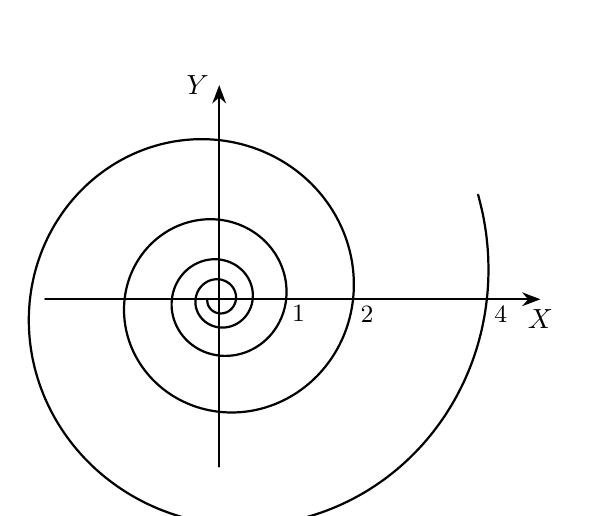
\begin{tikzpicture}[scale=0.85, >=Stealth, line cap=round, line join=round]
  % 座標軸
  \draw[thick, ->] (-2.6, 0) -- (4.8, 0) node[below] {$X$};
  \draw[thick, ->] (0, -2.5) -- (0, 3.2) node[left] {$Y$};
  % 螺線 r = 2^(\theta / 2\pi)
  \draw[thick, domain=-900:742, samples=400, smooth, variable=\t]
    plot (\t : {2^(\t/360)});
  % 交點刻度標記
  \node[below right, inner sep=1.5pt] at (1.02, -0.02) {\small $1$};
  \node[below right, inner sep=2pt] at (2.02, -0.02) {\small $2$};
  \node[below right, inner sep=2pt] at (4.02, -0.02) {\small $4$};
\end{tikzpicture}
\caption*{圖 3-1}\label{fig:b5s-1-3-1}
\end{figure}
\end{example}

在上例中我們看到了「$r - 2^{\theta/2\pi} = 0$」與上圖「螺線」間的對應。\textbf{那麼我們問：一個 $r$ 與 $\theta$ 間的一般關係式}
\begin{equation}\label{eq:b5s-1-3-2}
  g(r, \theta) = 0 \tag{2}
\end{equation}
\textbf{是否也正好對應一條極平面上的曲線？}

事實上這個對應在極座標是稍有一些困難的。

\medskip
\noindent\textbf{困難 1：}在上述例 1 $r - 2^{\theta/2\pi} = 0$ 中碰巧有 $r = 2^{\theta/2\pi} > 0$，我們未遭遇任何困難便得到該式與螺線間的良好對應。但一般情形下如果滿足 $g(r, \theta) = 0$ 中的某些 $r$ 會 $< 0$，我們怎樣處理？

\medskip
\begin{example}\label{ex:b5s-1-3-2}
$r = \cos\theta$

\begin{center}
\renewcommand{\arraystretch}{1.6}
\setlength{\tabcolsep}{4.5pt}
\small
\begin{tabular}{c|cccccccccccccc}
$\theta$ & $\cdots\cdots$ & $0,$ & $\dfrac{\pi}{6},$ & $\dfrac{\pi}{4},$ & $\dfrac{\pi}{3},$ & $\dfrac{\pi}{2},$ & $\dfrac{2\pi}{3},$ & $\dfrac{3\pi}{4},$ & $\dfrac{5\pi}{6},$ & $\pi,$ & $\dfrac{5\pi}{4},$ & $\dfrac{3\pi}{2},$ & $\dfrac{7\pi}{4},$ & $2\pi$ \\[4pt]
\hline
$r$ & $\cdots\cdots$ & $1,$ & $\dfrac{\sqrt{3}}{2},$ & $\dfrac{\sqrt{2}}{2},$ & $\dfrac{1}{2},$ & $0,$ & $-\dfrac{1}{2},$ & $-\dfrac{\sqrt{2}}{2},$ & $-\dfrac{\sqrt{3}}{2},$ & $-1,$ & $-\dfrac{\sqrt{2}}{2},$ & $0,$ & $\dfrac{\sqrt{2}}{2},$ & $1$
\end{tabular}
\end{center}

當我們從 $\theta = 0$ 起開始描點，到 $\theta = \dfrac{\pi}{2}$ 前，$r$ 都 $> 0$，得到圖 3-2 中上半圓弧 $\wideparen{ABO}$。可是一旦 $\theta$ 過了 $\dfrac{\pi}{2}$，$r$ 值變負，例如 $\theta = \dfrac{2\pi}{3}$ 時 $r = -\dfrac{1}{2} < 0$，這時要是把點描到沿原來 $\dfrac{2\pi}{3}$ 角終邊 $\vec{OQ}$ 的逆方向 $\vec{OQ'}$ 距離極點 $\dfrac{1}{2}$ 處，則得點 $P$（如圖 3-2）。

\begin{figure}[H]
\centering
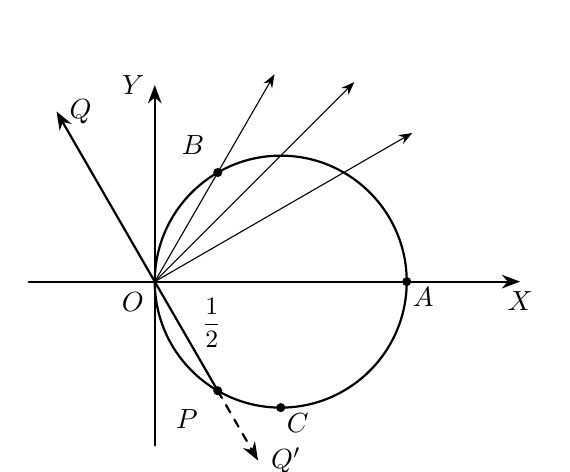
\begin{tikzpicture}[scale=3.2, >=Stealth, line cap=round, line join=round]
  % 座標軸
  \draw[thick, ->] (-0.5, 0) -- (1.45, 0) node[below] {$X$};
  \draw[thick, ->] (0, -0.65) -- (0, 0.78) node[left] {$Y$};
  \node[below left, inner sep=2pt] at (-0.02, -0.02) {$O$};

  % 圓 r = cos\theta (圓心 (0.5, 0)，半徑 0.5)
  \draw[thick] (0.5, 0) circle (0.5);

  % 第一象限描點射線
  \draw[->, thin] (0, 0) -- (30:1.18);
  \draw[->, thin] (0, 0) -- (45:1.12);
  \draw[->, thin] (0, 0) -- (60:0.95);

  % 第二象限射線 OQ (120度) 與第四象限逆方向射線 OQ' (300度)
  \draw[thick, ->] (0, 0) -- (120:0.78) node[right, xshift=1pt] {$Q$};
  \draw[thick] (0, 0) -- (300:0.5);
  \draw[thick, dashed, ->] (300:0.5) -- (300:0.82) node[right, xshift=1pt] {$Q'$};

  % 圓周各點標記
  \fill (1, 0) circle (0.018) node[below right, inner sep=2pt] {$A$};
  \fill (60:0.5) circle (0.018);
  \node[above left, inner sep=1.5pt] at (66:0.53) {$B$};
  \fill (300:0.5) circle (0.018);
  \node[below left, inner sep=2pt] at (292:0.52) {$P$};
  \fill (315:0.7071) circle (0.018) node[below right, inner sep=2pt] {$C$};

  % OP 長度 1/2 標記
  \node at (324:0.28) {\small $\dfrac{1}{2}$};
\end{tikzpicture}
\caption*{圖 3-2}\label{fig:b5s-3-2}
\end{figure}

現在採用上述方式\textbf{只要在 $\theta$ 終邊的方向上 $r$ 值變負，便把點描到 $\theta$ 終邊的逆方向上}，即當 $\theta$ 從 $\dfrac{\pi}{2}$ 轉到 $\pi$ 時我們得到下半圓弧 $\wideparen{OCA}$。

綜合起來，當 $\theta$ 從 $0$ 到 $\pi$ 時，滿足
\[
  r = \cos\theta
\]
的點 $P[r, \theta]$ 描出了一個正圓。
\end{example}

採這例中的方式可彌補「困難 1」，換句話說，

\medskip
\noindent\textbf{規約：}\textbf{$r$ 若為負值，則 $[r, \theta]$ 所對應的點描在幅角為 $\theta + \pi$ 的終邊的方向上，其到原點的距離為 $|r|$。}

\medskip
如右圖 (3-3) 中 $\left[-3, \dfrac{\pi}{6}\right]$ 之點標在 $P$ 處。\textbf{$r$ 若為 $0$}，則不拘 $\theta$ 為何值，$[0, \theta]$ 所對應的點規定取成原點。

\begin{figure}[H]
\centering
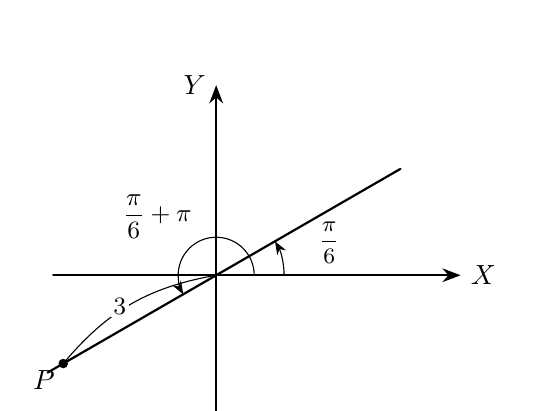
\begin{tikzpicture}[scale=1.15, >=Stealth, line cap=round, line join=round]
  % 座標軸
  \draw[thick, ->] (-1.8, 0) -- (2.7, 0) node[right] {$X$};
  \draw[thick, ->] (0, -1.6) -- (0, 2.1) node[left] {$Y$};

  % 射線 \pi/6 與 \pi/6 + \pi
  \draw[thick] (0, 0) -- (30:2.35);
  \draw[thick] (0, 0) -- (210:2.15);

  % 角弧 \pi/6
  \draw[->] (0.75, 0) arc (0:30:0.75);
  \node at (16:1.30) {\footnotesize $\dfrac{\pi}{6}$};

  % 角弧 \pi/6 + \pi
  \draw[->] (0.42, 0) arc (0:210:0.42);
  \node at (135:0.92) {\small $\dfrac{\pi}{6} + \pi$};

  % 點 P 與距離 3 的弧線標示
  \fill (210:1.95) circle (1.5pt);
  \draw[thin] (0, 0) to[bend right=20] (210:1.95);
  \node[fill=white, inner sep=1pt] at (198:1.12) {\small $3$};
  \node[below left, inner sep=2pt] at (210:1.98) {$P$};
\end{tikzpicture}
\caption*{圖 3-3}\label{fig:b5s-3-3}
\end{figure}

依照上述\textbf{規約}，我們知道了\textbf{兩個實數序對描述同一點 $P$ 的極座標之充要條件}，亦即

\medskip
\begin{prop}\label{prop:b5s-1-4}
當 $P \neq \text{原點}$ 時，$[r_1, \theta_1] = P = [r_2, \theta_2]$ 的充要條件是
\begin{equation}\label{eq:b5s-1-3-3}
  \begin{cases}
    r_1 = r_2 \\
    \theta_1 = \theta_2 + 2n\pi
  \end{cases}
  \qquad \text{或} \qquad
  \begin{cases}
    r_1 = -r_2 \\
    \theta_1 = (\theta_2 + \pi) + 2n\pi
  \end{cases} \tag{3}
\end{equation}
其中 $n$ 是任意整數。

〔至於 $P = \text{原點}$ 時，$[r_1, \theta_1] = P = [r_2, \theta_2] \Longleftrightarrow r_1 = r_2 = 0$〕

(3) 式合併起來，可縮寫為
\[
  \begin{cases}
    r_1 = (-1)^k r_2 \\
    \theta_1 = \theta_2 + k\pi
  \end{cases}
\]
其中 $k$ 為任意整數。
\end{prop}

\medskip
\subsubsection*{作業 8}
試描點畫出下列極平面上的軌跡圖形。
\begin{enumerate}[(i)]
  \item $r = \cos 2\theta$（四瓣）
  \item $r = \cos 3\theta$（三瓣）
\end{enumerate}
比較 (i), (ii) 與〔例 2〕$r = \cos\theta$ 三個軌跡各自要週而復始所須 $\theta$ 的最小範圍〔如 (i) 須 $\pi$\phantomsection\label{note:b5s-ch1-p25-hw8}\footnote{【原書註記/校訂】：原書第 25 頁作業 8 提示印作「〔如 (i) 須 $\pi$〕」。按在 $r \le 0$ 規約下，(ii) 三瓣玫瑰線 $r = \cos 3\theta$ 因 $\cos 3(\theta + \pi) = -\cos 3\theta$，故 $\theta$ 僅須歷經長度為 $\pi$ 之區間（如 $[0, \pi]$）即可描出完整三瓣而週而復始；至於 (i) 四瓣玫瑰線 $r = \cos 2\theta$ 因 $\cos 2(\theta + \pi) = \cos 2\theta$，在 $[0, \pi]$ 上僅能描出兩瓣之長，須歷經 $2\pi$ 方能描出完整四瓣。原書括號提示中「(i)」應為「(ii)」之筆誤。}〕。

\medskip
\subsubsection*{作業 9}
試描點畫出下列極平面上的各個軌跡圖形
\begin{enumerate}[(i)]
  \item $r = \dfrac{2}{\cos\left(\theta - \dfrac{\pi}{3}\right)}$ \qquad （直線）
  \item $r = a, \ (a \neq 0)$ \qquad （圓）
  \item $r = \dfrac{2}{1 - \cos\theta}$ \qquad （拋物線）
\end{enumerate}

\medskip
\begin{definition*}
對一個 $r, \theta$ 的關係式
\begin{equation}\label{eq:b5s-1-3-4}
  g(r, \theta) = 0 \tag{4}
\end{equation}
考慮所有滿足這關係的 $r, \theta$ 所相應的點 $P[r, \theta]$，這些點 $P[r, \theta]$ 構成了極平面上的一個圖形 $\Gamma$。我們把 $\Gamma$ 稱為這個 $g(r, \theta) = 0$ 一式的軌跡，而 $g(r, \theta) = 0$ 稱為 $\Gamma$ 的一個\textbf{極座標方程式}或簡稱\textbf{極方程式}。
\end{definition*}

\medskip
\paragraph{注意：}
\begin{enumerate}[(i)]
  \item 根據甲段 $r \le 0$ 的規約，這個定義中，滿足 (2) 式的 $r, \theta$ 不受範圍的限制。
  \item $\Gamma$ 上一個點 $P$ 有許多極座標 $[r_1, \theta_1], [r_2, \theta_2], \cdots$（關係如 (2) 式\phantomsection\label{note:b5s-ch1-p26-note}\footnote{【原書註記/校訂】：原書第 26 頁注意 (ii) 印作「（關係如 (2) 式）」，惟描述同一點 $P$ 之各組極座標 $[r_1, \theta_1], [r_2, \theta_2]$ 間的關係式實為第 25 頁【命題 4】之 (3) 式；此外下句「滿足的話，稱 $g(r, \theta) = 0$ 為良性的）」末尾多一右括號，轉錄時保留原貌並特此註明。}），當 $g(r, \theta) = 0$ 為 $\Gamma$ 的極方程式時\textbf{不一定}每一數對 $(r_1, \theta_1), (r_2, \theta_2), \cdots\cdots$ 都要滿足
  \[
    g(r_1, \theta_1) = g(r_2, \theta_2) = \cdots\cdots = 0.
  \]
  滿足的話，稱 $g(r, \theta) = 0$ 為\textbf{良性的}）

  如\textbf{〔例 1〕}螺線 $\Gamma : r = 2^{\theta/2\pi}$ 中，$P[1, 0]$ 是在 $\Gamma$ 上，而 $P$ 另有 $[1, 2\pi]$ 作為 $P$ 的極座標，但數對 $[1, 2\pi]$ 不滿足 $r = 2^{\theta/2\pi}$，意即
  \[
    1 \neq 2^{2\pi/2\pi} = 2
  \]
  \textbf{這是用極方程式描寫圖形的多種困難（如以後交點問題及對稱性判斷等）的起源}，這在下一節中我們要引入極圖觀點來詳細論述。
\end{enumerate}

\subsubsection*{乙、直線與圓的極方程式}\label{subsec:b5s-1-3-b}

我們已知道如何從極方程式描點以求圖形，但實際上更需要的是要把一些基本圖形如直線，圓，二次錐線等以極方程式表示出來。

下面兩論例我們考慮直線與圓的情形：

\medskip
\begin{discussion}[直線的極方程式]\label{disc:b5s-1-3}

對直線 $L$ 的一般式
\begin{equation}\label{eq:b5s-1-3-5}
  ax + by + c = 0 \tag{5}
\end{equation}
其中 $(x, y)$ 表直線 $L$ 上點的直角座標，根據 \S I-1 的變換式
\begin{equation}\label{eq:b5s-1-3-6}
  \begin{cases}
    x = r\cos\theta \\
    y = r\sin\theta
  \end{cases}
  \qquad \text{〔註〕}\footnotemark \tag{6}
\end{equation}
\footnotetext{〔原書註〕：當初提出 (6) 式時我們並未考慮到 $r \le 0$ 的規約。因此，(7) 式中 $r \le 0$ 之解 $[r, \theta]$ 是否也在 $L$ 上呢？對於這個問題我們只須考慮 (6) 式在 $r \le 0$ 規約下是否仍然成立即可。從這一點我們又可看出我們為何要作 \S I-3 甲段那樣的規約了。（見習題 I-3 第 6 題）}
其中 $[r, \theta]$ 表相應的極座標。顯然，以 (6) 式代入 (5) 式所得的
\[
  ar\cos\theta + br\sin\theta + c = 0
\]
\begin{equation}\label{eq:b5s-1-3-7}
  \text{或} \qquad r(a\cos\theta + b\sin\theta) + c = 0 \tag{7}
\end{equation}
便是\textbf{直線的一般極座標方程式}。

若用\textbf{向量處理法線式的觀點}，自原點引 $L$ 的垂線 $OA$，$A$ 為垂足，$\vect{u}$ 為 $OA$ 線上，矢角 $\omega$ 在 $0$ 與 $\pi$ 之間的單位法向量。（$\omega$ 稱為法向角）。設 $p = \pm\overline{OA}$ 其 $+$ 或 $-$ 號依 $\vect{u}$ 與 $\vec{OA}$ 同向或異向而定，則
\[
  P[r, \theta] \in L
\]
的充要條件是
\[
  \vec{OP} \cdot \vect{u} = p
\]
亦即
\[
  r\cos(\theta - \omega) = p
\]
或寫成
\begin{equation}\label{eq:b5s-1-3-8}
  r = \frac{p}{\cos(\theta - \omega)} \tag{8}
\end{equation}
這是一個\textbf{比較有幾何意義}的\textbf{直線的極座標方程式}。

\begin{figure}[H]
\centering
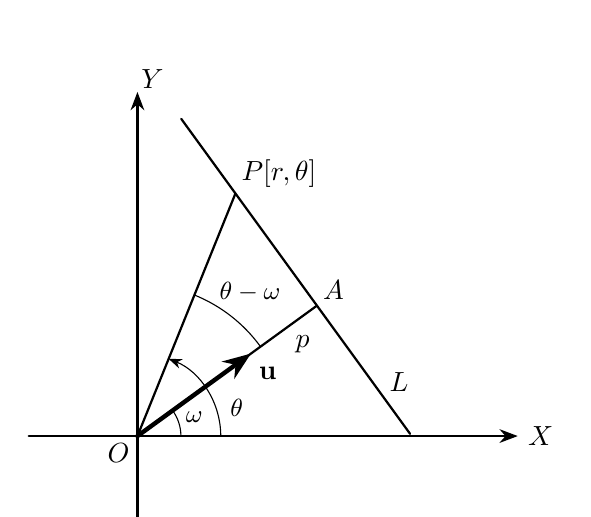
\begin{tikzpicture}[scale=1.15, >=Stealth, line cap=round, line join=round]
  % 座標軸
  \draw[thick, ->] (-1.2, 0) -- (4.2, 0) node[right] {$X$};
  \draw[thick, ->] (0, -1.0) -- (0, 3.8) node[above right, inner sep=1pt] {$Y$};
  \node[below left, inner sep=2pt] at (-0.02, -0.02) {$O$};

  % 定義法向角 \omega = 36度, p = 2.45
  \coordinate (A) at (36:2.45);
  % 直線 L 垂直於 OA (方向 126度 與 -54度)
  \draw[thick] ($(A) + (-54:1.75)$) -- ($(A) + (126:2.55)$);
  \node[above right, inner sep=2pt] at ($(A) + (-54:1.25)$) {$L$};

  % 垂足 A 與法線段 OA、單位法向量 u
  \draw[thick] (0, 0) -- (A);
  \draw[ultra thick, ->] (0, 0) -- (36:1.55);
  \node[below right, inner sep=2pt] at (33:1.52) {$\vect{u}$};
  \node[below right, inner sep=2pt] at (35:2.05) {$p$};
  \node[above right, inner sep=2pt] at (A) {$A$};

  % 直線上點 P[r, \theta] (\theta = 68度, r = 2.45 / cos(32度) = 2.889)
  \coordinate (P) at (68:2.889);
  \draw[thick] (0, 0) -- (P);
  \node[above right, inner sep=2pt] at (P) {$P[r, \theta]$};

  % 角弧 \omega (0 到 36度)
  \draw (0.48, 0) arc (0:36:0.48);
  \node at (18:0.66) {\small $\omega$};

  % 角弧 \theta (0 到 68度)
  \draw[->] (0.92, 0) arc (0:68:0.92);
  \node at (16:1.14) {\small $\theta$};

  % 角弧 \theta - \omega (36 到 68度)
  \draw (36:1.68) arc (36:68:1.68);
  \node at (52:2.02) {\small $\theta - \omega$};
\end{tikzpicture}
\end{figure}

\noindent\textbf{特殊情形：}
\begin{enumerate}[(i)]
  \item 當 $L$ 平行於極軸時，$\omega = \dfrac{\pi}{2}$，故得
  \[
    r = \frac{p}{\cos\left(\theta - \dfrac{\pi}{2}\right)} = \frac{p}{\sin\theta}
  \]
  即 \qquad $r\sin\theta = p$
  \item 當 $L$ 垂直於極軸時，$\omega = 0$，故得
  \[
    r\cos\theta = p.
  \]
\end{enumerate}
\end{discussion}

\begin{discussion}[圓的極方程式]\label{disc:b5s-1-4}
考慮一圓 $\Gamma$，圓心 $C$ 之極座標為 $[\rho, \alpha]$，半徑為 $a$，則
\[
  \text{「}P[r, \theta] \in \Gamma\text{」}
\]
的充要條件為
\[
  \text{「}\overline{CP} = a \text{（即 } \overline{CP}^2 = a^2\text{）」}
\]
根據餘弦定律，這充要條件可寫成
\begin{equation}\label{eq:b5s-1-3-9}
  r^2 + \rho^2 - 2\rho r\cos(\theta - \alpha) = a^2 \tag{9}
\end{equation}
這便是\textbf{圓的極方程式}。\hfill$\#$

\begin{figure}[H]
\centering
\begin{tikzpicture}[scale=1.15, >=Stealth, line cap=round, line join=round]
  % 極點 O 與極軸 OX
  \coordinate (O) at (0, 0);
  \node[below left, inner sep=2pt] at (O) {$O$};
  \draw[thick, ->] (O) -- (5.5, 0) node[above, yshift=2pt] {$X$} node[below, yshift=-2pt, xshift=-6pt] {\small 極軸};

  % 圓心 C[\rho, \alpha] (\alpha = 18度, \rho = 3.65, 半徑 a = 1.25)
  \coordinate (C) at (18:3.65);
  \draw[thick] (C) circle (1.25);
  \fill (C) circle (1.5pt);
  \node[below, yshift=-3pt, xshift=4pt] at (C) {$C[\rho, \alpha]$};

  % 圓上點 P[r, \theta]
  \coordinate (P) at ($(C) + (92:1.25)$);
  \fill (P) circle (1.5pt);
  \node[above, yshift=2pt] at (P) {$P[r, \theta]$};

  % 連線 OC, OP 與虛線半徑 CP
  \draw[thick] (O) -- (C);
  \draw[thick] (O) -- (P) node[midway, above left, inner sep=2pt] {$r$};
  \draw[thick, dashed] (C) -- (P) node[midway, right, xshift=2pt] {$a$};

  % 角弧 \alpha 與 \theta - \alpha
  \draw[->] (1.00, 0) arc (0:18:1.00);
  \node at (9:1.24) {\small $\alpha$};
  \draw (18:1.25) arc (18:36.8:1.25);
  \node at (26.5:1.68) {\footnotesize $\theta - \alpha$};
\end{tikzpicture}
\end{figure}
\end{discussion}
\paragraph{注意：}
在這兩論例中，直線或圓上一點 $P$ 的任何極座標 $[r, \theta]$，$[-r, \theta + \pi]$，$[r, \theta + 2\pi]\cdots\cdots$ 等中每一數對都分別滿足它們的極方程式 (8), (9) 式，其道理留當\textbf{作業}。這樣的極方程式，我們稱為\textbf{良性的極方程式}，這現象不是始終都成立的（如 $r = 2^{\theta/2\pi}$）。\textbf{但當它成立時，許多用極方程式討論的可能的疵漏都可避免}（見下面\textbf{作業}及下節交點問題）\phantomsection\label{note:b5s-ch1-p28-fn}\footnote{〔原書註〕：此處我們視圓 $x^2 + y^2 = a^2$ 的極方程式為 $r^2 = a^2$，因為開方會去掉 $r = -a$ 使得剩下的方程式 $r = a$ 不為良性。（【編按】：原書第 28 頁頁底印有此則「〔註〕」，惟正文中未標註對應之「〔註〕」號，依文義係補充說明圓之良性極方程式，故綴於此段末尾。）}。

\medskip
\begin{example}\label{ex:b5s-1-3-3}
設一圓通過以下列的直角座標表其位置的三個點
\[
  P_1(0, 0), \quad P_2(1, 0), \quad P_3(0, 2)
\]
求此圓的極方程式。
\end{example}
\paragraph{【解】}
\begin{enumerate}[(i)]
  \item 我們的方法是找出這三點的極座標
  \[
    P_1 = (0, 0) = [0, 0], \qquad P_2 = (1, 0) = [1, 0],
  \]
  \[
    P_3 = (0, 2) = \left[2, \frac{\pi}{2}\right]
  \]
  然後將這些數對分別代入圓的一般方程式
  \begin{equation}\label{eq:b5s-1-3-10}
    r^2 + \rho^2 - 2\rho r\cos(\theta - \alpha) = a^2 \qquad (\text{取 } a > 0) \tag{10}
  \end{equation}
  得：〔這些數對為什麼滿足 (10) 式？〕
  \[
    \begin{cases}
      \rho^2 = a^2 \\
      1 + \rho^2 - 2\rho\cos\alpha = a^2 \\
      4 + \rho^2 - 4\rho\cos\left[\dfrac{\pi}{2} - \alpha\right] = a^2
    \end{cases}
  \]
  簡化得 $1 - 2a\cos\alpha = 0$，及 $1 - a\sin\alpha = 0$\phantomsection\label{note:b5s-ch1-p29-ex3}\footnote{【原書註記/校訂】：原書第 29 頁由聯立方程組 $\rho^2 = a^2$（取 $\rho = a > 0$）消去常數項後，直接將 $\rho$ 寫作 $a$ 而得 $1 - 2a\cos\alpha = 0$ 及 $1 - a\sin\alpha = 0$，並代入 (10) 式化為 $r = 2a\cos(\theta - \alpha)$。}

  代入 (10) 式後可化簡得
  \begin{align*}
    r &= 2a\cos(\theta - \alpha) \\
      &= (2a\cos\alpha)\cos\theta + (2a\sin\alpha)\sin\theta
  \end{align*}
  亦即 \qquad $r = \cos\theta + 2\sin\theta$ \qquad 〔註〕\footnote{〔原書註〕：在得到此式前我們將兩端消去了一個 $r$ 但可以驗得這個操作並未損失原點之根。}

  \item 但這方法為什麼是正確的？換句話說為什麼上述數對會滿足 (10) 式？例如 $P_3$ 有其他極座標 $\left[2, \dfrac{\pi}{2} + 2\pi\right], \left[-2, \dfrac{\pi}{2} - \pi\right], \cdots$ 等，我們知道 $P_3$ 在圓上時，只知 $P_3$ 的各極座標中\textbf{有一個}它的數對會滿足 (10) 式。幸好本例前的「注意」告訴我們若 $P$ 在圓上，則 $P$ 的每一個極座標所含的數對都會滿足 (10) 式，故上述討論無誤。\hfill$\#$
\end{enumerate}

從最後這個例子中，我們注意到：以前採用直角座標方程式描述曲線時從不會發生的問題，現在採用極座標時便有了困難，換句話說，一般時候
\[
  g(r, \theta) = 0
\]
所代表的軌跡上的一點 $P = [r_0, \theta_0] = [-r_0, \theta_0 + \pi] = [r_0, \theta_0 + 2\pi] = \cdots\cdots$ 中只知至少有一組數對是滿足 $g(r, \theta) = 0$，譬如可能 $g(r_0, \theta_0) = 0$，但 $g(-r_0, \theta_0 + \pi) \neq 0, \ g(r_0, \theta_0 + 2\pi) \neq 0$。

% =========================================================================
% 習題 I-3
% =========================================================================
\subsubsection*{習題 I-3}\label{sec:b5s-ex1-3}

\begin{enumerate}[1.]
  \item 求下列直線之極方程式
  \begin{enumerate}[(a)]
    \item 斜率為 $3$，$Y$ 截距為 $-2$
    \item 斜率為 $-2$，到原點距離為 $5$（兩解）
    \item $X, Y$ 兩軸截距分別為 $2, -6$。
  \end{enumerate}

  \item 求下列圓之極方程式
  \begin{enumerate}[(a)]
    \item 圓心在 $(-2, 1)$，半徑為 $5$
    \item 通過 $(0, 0), (u, 0), (0, v)$ 三點 $(u, v \neq 0)$
    \item 以 $(4, 1), (2, 3)$ 連線為直徑
  \end{enumerate}

  \item 設 $P[r_0, \theta_0]$ 在直線
  \[
    r = \frac{p}{\cos(\theta - \omega)}
  \]
  上，是否必然可得
  \[
    r_0 = \frac{p}{\cos(\theta_0 - \omega)}\text{？}
  \]
  解釋其道理。

  \item 想求一直線與一圓的交點，是否解其相應的極方程式
  \[
    \begin{cases}
      r = \dfrac{p}{\cos(\theta - \omega)} \\[8pt]
      r^2 + \rho^2 - 2\rho r\cos(\theta - \alpha) = a^2
    \end{cases}
  \]
  必可獲得所有交點？其道理何在？

  \item 求一通過 $(0, 1)$ 而與 $2x + \sqrt{3}y = 1$ 相切之圓的極方程式。

  \item 在論例 3 中我們其實已經得到一個把直角座標方程式變換成極方程式的一般方法。試將下列事實顯示出來：
  \begin{enumerate}[(a)]
    \item $(x, y)$ 與 $[r, \theta]$ 表相同點的充要條件是
    \[
      \begin{cases}
        x = r\cos\theta \\
        y = r\sin\theta
      \end{cases}
    \]
    特別注意上式中 $r \le 0$ 也成立。
    \item 若圖形 $\Gamma$ 的直角座標方程式是 $f(x, y) = 0$，則它的極座標方程式是 $f(r\cos\theta,\allowbreak r\sin\theta) = 0$，其逆亦真。
    \item 由上述方法得來的極方程式 $f(r\cos\theta, r\sin\theta) = 0$ 是良性的，即，若 $P$ 在 $f(r\cos\theta, r\sin\theta) = 0$ 之圖形上，則 $P$ 的每一個極座標 $[r_0, \theta_0]$ 必然都滿足 $f(r_0\cos\theta_0, r_0\sin\theta_0) = 0$。
  \end{enumerate}

  \item 試從圓的直角座標方程式再導出圓的極方程式
  \[
    r^2 + \rho^2 - 2\rho r\cos(\theta - \alpha) = a^2.
  \]
  從這個導引過程，第 6 題直接告訴我們：圓方程式是「良性的」方程式。

  \stepcounter{enumi}\item[\textbf{*8.}]
  \begin{enumerate}[(a)]
    \item 已知極平面上兩點 $A$、$B$，其中 $A$ 為二直線
    \[
      r\cos\left(\theta - \frac{\pi}{6}\right) = 3, \quad r\sin\theta = 3 \text{ 的交點，} B \text{ 為 } \left[2, \frac{5\pi}{6}\right]\text{；}
    \]
    試求出通過 $A, B$ 兩點的直線極方程式
    \item 由 (a) 所得直線 $AB$ 有一動點 $P[r_1, \theta_1]$，現以 $OP$ 線段為一邊，作正三角形 $\triangle OPQ$，（$O$ 為極），試求出頂點 $Q$ 之軌跡決定的極方程式。
  \end{enumerate}

  \item 試求出過三點 $[0, 0], [\alpha, 0], \left[\beta, \dfrac{\pi}{2}\right]$ 之圓的極方程式。$(\alpha\beta \neq 0)$，
  \[
    [r = \alpha\cos\theta + \beta\sin\theta]
  \]

  \item[\textbf{*10.}] 試利用習題 I-1 第 5 題的解法導出平面上三點 $[r_1, \theta_1], [r_2, \theta_2], [r_3, \theta_3]$ 點所決定三角形的面積大小。
\end{enumerate}
% =========================================================================
% §I-4 交點問題 (Pages 31--45)
% =========================================================================
\subsection{交點問題}\label{sec:b5s-1-4}

用極座標方程式來描寫曲線，還存在其他一些困難。

\medskip
\setcounter{example}{0}
\begin{example}\label{ex:b5s-1-4-1}
考慮兩方程式
\begin{equation}
\begin{cases}
r = 2^{\theta / 2\pi} \\[4pt]
\theta = \dfrac{2\pi}{3}
\end{cases}
\tag{1}
\end{equation}

\begin{figure}[H]
\centering
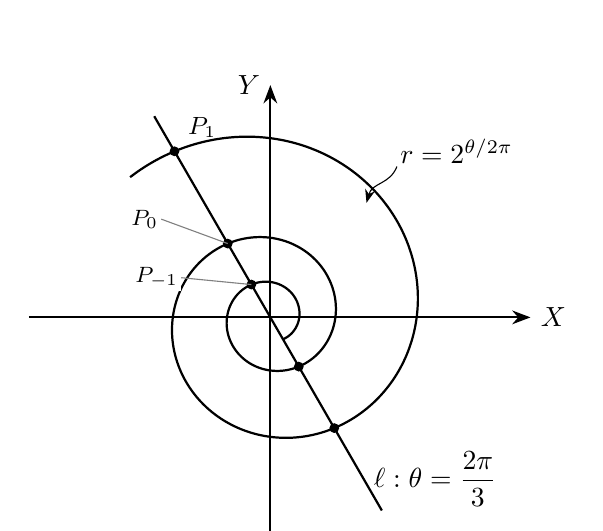
\begin{tikzpicture}[scale=1.18, >=Stealth]
  % Axes
  \draw[->, thick] (-2.6, 0) -- (2.8, 0) node[right] {$X$};
  \draw[->, thick] (0, -2.4) -- (0, 2.5) node[left] {$Y$};

  % Line l: \theta = 2\pi/3 (120 deg and -60 deg)
  \draw[thick] (120:2.5) -- (-60:2.4) node[right, pos=0.92] {$\ell : \theta = \dfrac{2\pi}{3}$};

  % Spiral r = 2^{\theta / 2\pi}
  \draw[thick, domain=-420:495, samples=300, smooth, variable=\t]
    plot (\t : {0.70 * exp(\t/360 * ln(2.25))});

  % Intersection points on 120 deg ray (with short leader lines to clear space)
  \fill (120:0.408) circle (1.5pt);
  \draw[thin, gray] (120:0.408) -- (156:1.05) node[left, fill=white, inner sep=1pt, text=black, font=\footnotesize] {$P_{-1}$};

  \fill (120:0.917) circle (1.5pt);
  \draw[thin, gray] (120:0.917) -- (138:1.58) node[left, fill=white, inner sep=1pt, text=black, font=\footnotesize] {$P_0$};

  \fill (120:2.064) circle (1.5pt);
  \node[above right=2pt, font=\small] at (120:2.064) {$P_1$};

  % Intersection points on -60 deg ray
  \fill (-60:0.612) circle (1.5pt);
  \fill (-60:1.376) circle (1.5pt);

  % Label for spiral with pointer
  \draw[<-, thin] (50:1.61) .. controls (53:1.82) and (48:1.92) .. (50:2.12)
    node[above right, inner sep=1pt] {$r = 2^{\theta / 2\pi}$};
\end{tikzpicture}
\caption*{圖 4-1}
\end{figure}

恰得一公解\quad $r = 2^{1/3}$，$\theta = \dfrac{2\pi}{3}$

記 $P_0 = \left[2^{\frac{1}{3}}, \dfrac{2\pi}{3}\right]$，但兩式在極平面上一表螺狀線〔見 \S I-3 例 1〕，一表幅角為 $\dfrac{2\pi}{3}$ 的終邊。（其實依照上段「規約」，$r$ 值可負，$\theta = \dfrac{2\pi}{3}$ 應推廣為整條直線 $\ell$）兩線有無窮多個交點，如圖 4-1。

換句話說，由聯立方程式 (1) 所求得的公解未能示出兩相應軌跡的所有交點。\hfill$\#$
\end{example}

\medskip
\begin{example}\label{ex:b5s-1-4-2}
考慮兩方程式
\begin{equation}
\begin{cases}
r = 2^{\theta / 2\pi} \\[4pt]
r = 2^{(\theta + 2\pi) / 2\pi}
\end{cases}
\tag{2}
\end{equation}
\end{example}
\paragraph{【解】}
欲求其公解：
\[
2^{\theta / 2\pi} = 2^{(\theta + 2\pi) / 2\pi}
\]
\[
\theta / 2\pi = (\theta + 2\pi) / 2\pi \qquad \text{〔因指數函數為單調〕}
\]
\[
\theta = \theta + 2\pi
\]
顯然沒有 $\theta$ 能滿足上式，故聯立方程式 (2) 無解。\hfill$\#$

可是 $r = 2^{\theta / 2\pi}$ 與 $r = 2^{(\theta + 2\pi) / 2\pi}$ 兩式竟然描出了極平面上同一螺狀軌跡。

這兩個例子顯示，極平面軌跡方程無法足夠良好地描述其上的曲線；換句話說：

\medskip
\noindent\textbf{困難 2}：\textbf{在代數上聯立方程式的求解，原對應於幾何上圖形間的交點，可是這一重要的轉化關係採用極座標時卻發生了困難。}

\begin{figure}[H]
\centering
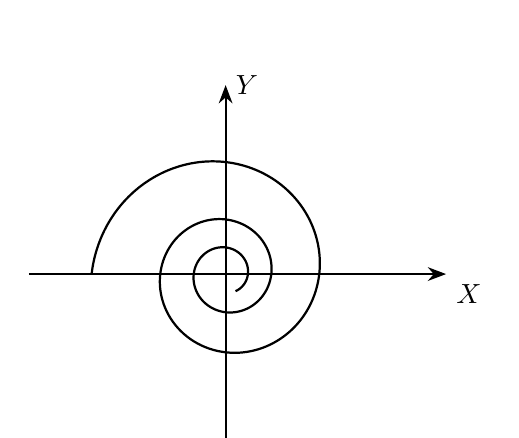
\begin{tikzpicture}[scale=1.0, >=Stealth]
  \draw[->, thick] (-2.5, 0) -- (2.8, 0) node[below right] {$X$};
  \draw[->, thick] (0, -2.2) -- (0, 2.4) node[right] {$Y$};
  \draw[thick, domain=-420:540, samples=300, smooth, variable=\t]
    plot (\t : {0.58 * exp(\t/360 * ln(2.05))});
\end{tikzpicture}
\caption*{圖 4-2\quad 重合的兩個螺狀線}
\end{figure}

其實這一困難要追溯的話原起自平面上同一個點，不只對應一個極座標。換句話說：\textbf{極座標不是一個足夠良好的座標}；從這裏引出的困難，除了交點問題外，還有對稱性等一些伴隨而來的副作用，可是極座標在描述這些曲線時又不失為好的描述。〔例如\underline{牛頓}採二次曲線的極座標表示利用微分，而自\underline{刻卜勒}三大觀測結果導出萬有引力定律，這是科學史上的一件大事〕

我們以下例來表明交點問題解決的方法。

\medskip
\begin{example}\label{ex:b5s-1-4-3}
求在極平面上下列兩方程式
\[
\begin{cases}
r = 2^{\theta / 2\pi} \\[4pt]
\theta = \dfrac{2\pi}{3}
\end{cases}
\]
所代表的兩條軌跡間所有的交點。

\begin{figure}[H]
\centering
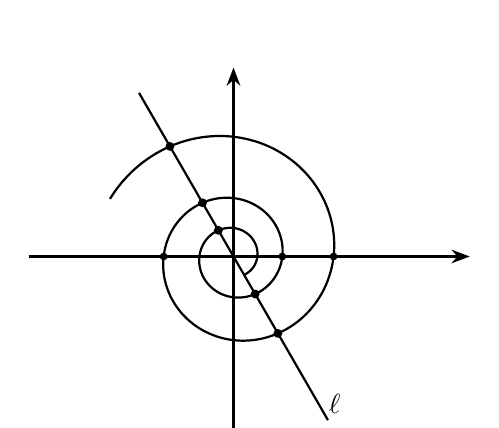
\begin{tikzpicture}[scale=1.0, >=Stealth]
  \draw[->, thick] (-2.6, 0) -- (3.0, 0);
  \draw[->, thick] (0, -2.3) -- (0, 2.4);
  \draw[thick] (120:2.4) -- (-60:2.4) node[right, pos=0.95] {$\ell$};
  \draw[thick, domain=-420:515, samples=300, smooth, variable=\t]
    plot (\t : {0.62 * exp(\t/360 * ln(2.05))});

  % Intersections on 120 deg and -60 deg rays
  \foreach \t in {-240, 120, 480, -60, 300} {
    \fill (\t : {0.62 * exp(\t/360 * ln(2.05))}) circle (1.6pt);
  }
  % Intersections on X-axis (0 and 180 deg)
  \foreach \t in {0, 180, 360} {
    \fill (\t : {0.62 * exp(\t/360 * ln(2.05))}) circle (1.4pt);
  }
\end{tikzpicture}
\caption*{圖 4-3}
\end{figure}
\end{example}
\paragraph{【解法】}
\begin{enumerate}[label=(\roman*), leftmargin=2.5em]
\item 求
\[
\begin{cases}
r = 2^{(\theta + 2n\pi) / 2\pi} \\[4pt]
\theta = \dfrac{2\pi}{3}
\end{cases}
\]
的公解，得
\[
\begin{aligned}
r &= 2^{(\frac{2\pi}{3} + 2n\pi) / 2\pi} = 2^{n + \frac{1}{3}} \\[4pt]
\theta &= \frac{2\pi}{3}
\end{aligned}
\]
亦即對任意整數 $n$，$\left[2^{n + \frac{1}{3}}, \dfrac{2\pi}{3}\right]$ 皆為兩軌跡的交點。（$n$ 為任意整數），但我們曾為了方便而容許 $r \le 0$，因此 $\theta = \dfrac{2\pi}{3}$ 代表整條直線 $\ell$，而非只為一射線，故尚須考慮上圖第四象限中的各個交點。

\item 再求
\[
\begin{cases}
r = -2^{(\theta + \pi + 2n\pi) / 2\pi} \\[4pt]
\theta = \dfrac{2\pi}{3}
\end{cases}
\]
的公解，得
\[
\begin{aligned}
r &= -2^{(\frac{2\pi}{3} + \pi + 2n\pi) / 2\pi} = -2^{n + \frac{5}{6}} \\[4pt]
\theta &= \frac{2\pi}{3}
\end{aligned}
\]
亦即對任意整數 $n$，$\left[-2^{n + \frac{5}{6}}, \dfrac{2\pi}{3}\right]$ 都是兩軌跡的交點。

\item $r = 2^{(\theta + 2n\pi) / 2\pi}$\phantomsection\label{note:b5s-ch1-p38-exp}\footnote{【原書註記/校訂】：原書第 34 頁 (iii) 處指數分子部分有重印墨跡（作 $2^{(\theta + 2n\pi)/2\pi}$ 或 $2^{(\theta + k\pi)/2\pi}$），意指無論平移多少週期，指數函數恆正而永不為 $0$。}，永不為 $0$，故原點並非交點。
\end{enumerate}

合併起來知 $\left[2^{n + \frac{1}{3}}, \dfrac{2\pi}{3}\right]$ 與 $\left[-2^{n + \frac{5}{6}}, \dfrac{2\pi}{3}\right]$ 為兩軌跡間所有交點，其中 $n$ 為任意整數。\hfill$\#$

\medskip
這個例子所用的方法一般化後敘述如下：

\medskip
\setcounter{theorem}{0}
\begin{theorem}\label{thm:b5s-1-4-1}
給定兩個極方程式
\begin{equation}
\begin{cases}
g(r, \theta) = 0 \\[4pt]
h(r, \theta) = 0
\end{cases}
\tag{3}
\end{equation}
它們在極平面上的軌跡的所有交點，除原點外，若以極座標 $[r, \theta]$ 表示，則這些 $r, \theta$ 正好就是下列各聯立方程式的解
\begin{equation}
\begin{cases}
g(r, \theta + 2n\pi) = 0 \\[4pt]
h(r, \theta) = 0
\end{cases}
\quad \text{與} \quad
\begin{cases}
g(-r, \theta + \pi + 2n\pi) = 0 \\[4pt]
h(r, \theta) = 0
\end{cases}
\tag{4}
\end{equation}
（$n$ 為任意整數）

(4) 式合併起來，可縮寫成
\begin{equation}
\begin{cases}
g((-1)^k r, \theta + k\pi) = 0 \\[4pt]
h(r, \theta) = 0
\end{cases}
\tag{4$'$}
\end{equation}
（$k$ 為任意整數）
\end{theorem}

\noindent\underline{道理是這樣的}：若有點 $P'[r_0, \theta_0]$ 在 $\Gamma' : h(r, \theta) = 0$ 上，則 $P'$ 所有可能的極座標為
\[
[(-1)^k r_0, \theta_0 + k\pi] \qquad (\text{$k$ 為任意整數})
\]
而當 $P'$ 亦在 $\Lambda' : g(r, \theta) = 0$ 時，必有一個 $k_0$，使 $[(-1)^{k_0} r_0, \theta_0 + k_0\pi]$ 滿足
\[
g(r, \theta) = 0
\]
即有
\[
g((-1)^{k_0} r_0, \theta_0 + k_0\pi) = 0
\]
故 $[r_0, \theta_0]$ 為 (4$'$) 的公解。

反過來，若有 (4$'$) 的公解，則因 $g((-1)^k r, \theta + k\pi) = 0$ 亦為 $\Lambda'$ 的軌跡方程式，故所相應的點 $P_1[r_1, \theta_1]$ 同時落在
\[
\Lambda' : g((-1)^k r, \theta + k\pi) = 0
\]
與
\[
\Gamma' : h(r, \theta) = 0
\]
之上，亦即 $P_1[r_1, \theta_1] \in \Lambda' \cap \Gamma'$。\hfill$\#$

至於原點是否為其交點，須分別查看，是否存在 $\theta_1, \theta_2$ 使
\[
\begin{cases}
g(0, \theta_1) = 0 \\[4pt]
h(0, \theta_2) = 0
\end{cases}
\]

\medskip
\subsubsection*{習題 I-4}\label{sec:b5s-ex1-4}

求下列各聯立方程式在極平面上的所有交點：

\begin{enumerate}[label=\arabic*., leftmargin=2em]
\item $\begin{cases} r = 1 - \cos\theta & \text{〔心臟線〕} \\[4pt] r = \cos\theta & \text{〔圓〕} \end{cases}$
\item $\begin{cases} r = \dfrac{1}{1 - \cos\theta} & \text{〔拋物線〕} \\[8pt] r = 2\cos 2\theta & \text{〔四瓣玫瑰線〕} \end{cases}$
\item 先查表找 $\cos\theta = \theta^2$ 的逼近解〔$\theta$ 單位採取弧度制〕後求
\[
\begin{cases}
r = \theta^2 & \text{〔二次螺線〕} \\[4pt]
r = \cos\theta
\end{cases}
\]
在極平面上的所有交點。
\end{enumerate}

% =========================================================================
% § I-5 二次曲線的極方程式
% =========================================================================
\subsection{二次曲線的極方程式}
\label{sec:b5s-1-5}

\subsubsection*{甲、極方程式的導引}

現在我們利用三種非特異二次曲線所共通具有的準線性質來導出它們統一的極方程式。（由於準線性質實際上是非特異二次曲線的特徵性質，我們可以單純地從這特徵性質出發，而得二次曲線的極方程式），回想準線性質的意思：

\begin{figure}[H]
\centering
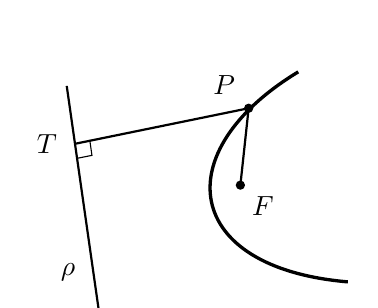
\begin{tikzpicture}[scale=1.05]
  % Directrix line \rho (tilted slightly as in original Fig 5-1)
  \coordinate (D1) at (-1.35, 1.45);
  \coordinate (D2) at (-0.95, -1.35);
  \draw[thick] (D1) -- (D2);
  \node[left=3pt] at (-1.03, -0.8) {$\rho$};

  % Conic curve \Gamma and Focus F
  \coordinate (F) at (0.75, 0.25);
  \fill (F) circle (1.6pt) node[below right=1pt] {$F$};

  % Draw smooth conic arc around F
  \draw[very thick] (1.45, 1.62) .. controls (-0.15, 0.65) and (0.05, -0.75) .. (2.05, -0.92);

  % Point P on the curve
  \coordinate (P) at (0.85, 1.18);
  \fill (P) circle (1.6pt) node[above left=2pt] {$P$};

  % Foot of perpendicular T on directrix \rho
  \coordinate (T) at (-1.25, 0.75);
  \draw[thick] (P) -- (T);
  \draw[thick] (P) -- (F);

  % Right angle mark at T
  \draw ($(T) + (0.18, 0.036)$) -- ($(T) + (0.205, -0.14)$) -- ($(T) + (0.025, -0.176)$);
  \node[left=3pt] at (T) {$T$};
\end{tikzpicture}
\caption*{圖 5-1}
\label{fig:b5s-5-1}
\end{figure}

固定平面上的一直線 $\rho$\phantomsection\label{note:b5s-ch1-p46-rho}\footnote{【原書註記/校訂】：原書以希臘字母 $\rho$ 表示準線（直線），並以斜體拉丁字母 $p$ 表示極點 $O$ 到準線 $\rho$ 的距離（見本頁末「設 $O$ 到 $\rho$ 的距離為 $p$」及圖 5-2），兩者字形相近但意義有別，正文嚴格區分之。}及 $\rho$ 外一點 $F$，設 $e > 0$ 為一定數，所有到 $F$ 點與到直線 $\rho$ 的比值為 $e$ 的點 $P$，亦卽
\[
  \frac{\overline{PF}}{\overline{PT}} = e \qquad \text{其中 $T$ 為自 $P$ 到 $\rho$ 的垂足，}
\]
所組成的軌跡，恰好就是所謂的非特異的二次曲線（正圓除外）。

若進一層加以分類，設上述軌跡為 $\Gamma$ 則
\begin{enumerate}[(i)]
  \item 當 $0 < e < 1$，$\Gamma$ 為正圓除外的橢圓
  \item 當 $e = 1$，$\Gamma$ 為拋物線
  \item 當 $e > 1$，$\Gamma$ 為雙曲線
\end{enumerate}

今取此定點 $F$ 為極 $O$，必要時把平面作一旋轉，不妨假設準線 $\rho$ 鉛垂而立於 $O$ 的左邊\footnote{（註）當然可使 $\rho$ 位於 $O$ 的右邊，但此時若 $e = 1$ 則所得的拋物線開口朝左，與我們第四冊的習慣不一。}，\underline{取水平向右的半射線}為極軸 $OX$，此時 $(O; \vec{OX})$ 構成一極座標系，設 $O$ 到 $\rho$ 的距離為 $p$。

由準線性質，設 $P[r, \theta]$ 為 $\Gamma$ 上一點，（此處 $[r, \theta]$ 為相關於 $(O; \vec{OX})$ 的極座標）\phantomsection\label{note:b5s-ch1-p46-paren}\footnote{【原書註記/校訂】：原書第 46 頁最末行「（此處 $[r, \theta]$ 為相關於 $(O; \vec{OX})$ 的極座標」跨頁接第 47 頁首行「則 $\frac{\overline{PO}}{\overline{PT}} = e$」時，漏印右括號「）」，茲予補齊。}，則
\[
  \frac{\overline{PO}}{\overline{PT}} = e
\]
但 $\overline{PO} = r$，$\overline{PT} = r\cos\theta + p$，故
\[
  \frac{r}{r\cos\theta + p} = e
\]
\[
  r = re\cos\theta + pe
\]
\begin{equation}
  r = \frac{pe}{1 - e\cos\theta} \tag{1} \label{eq:b5s-1-5-1}
\end{equation}
這就是非特異二次曲線的極方程式。\phantomsection\label{note:b5s-ch1-p47-fig52}\footnote{【原書註記/校訂】：原書圖 5-2 於極軸下方括弧標記為「$\cos\theta$」，按幾何關係 $\overline{OP}=r$，其水平投影長實為「$r\cos\theta$」（參見正文 $\overline{PT}=r\cos\theta+p$），圖中係略去或漏印 $r$，此處依原圖忠實重現並附註說明。}

\begin{figure}[H]
\centering
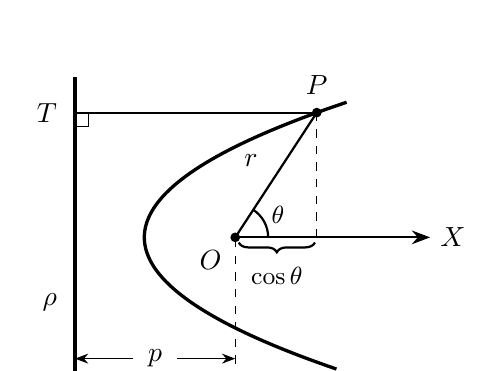
\begin{tikzpicture}[scale=1.1]
  % Directrix \rho at x = -1.85
  \draw[very thick] (-1.85, -1.65) -- (-1.85, 1.85);
  \node[left=3pt] at (-1.85, -0.75) {$\rho$};

  % Vertical dashed reference line through O(0,0)
  \coordinate (O) at (0, 0);
  \draw[dashed] (0, -1.65) -- (0, 0);

  % Polar axis OX
  \draw[thick, -Stealth] (O) -- (2.25, 0) node[right] {$X$};
  \fill (O) circle (1.6pt) node[below left=2pt] {$O$};

  % Conic arc matching Fig 5-2: x = -1.05 + 0.96 y^2 for y in [-1.52, 1.56]
  \draw[very thick, domain=-1.52:1.56, samples=80]
    plot ({-1.05 + 0.96*(\x)^2}, {\x});

  % Point P on the upper right of the arc: yP = 1.44 -> xP = 0.941
  \coordinate (P) at (0.941, 1.44);
  \coordinate (T) at (-1.85, 1.44);
  \coordinate (H) at (0.941, 0);

  \fill (P) circle (1.6pt) node[above=3pt] {$P$};

  % Segment PT and right angle mark at T(-1.85, 1.44)
  \draw[thick] (P) -- (T);
  \draw (-1.85, 1.28) -- (-1.69, 1.28) -- (-1.69, 1.44);
  \node[left=3pt] at (T) {$T$};

  % Radial segment OP and vertical dashed projection PH
  \draw[thick] (O) -- (P) node[pos=0.45, above left=2pt] {$r$};
  \draw[dashed] (P) -- (H);

  % Angle arc \theta (angle of P is atan2(1.44, 0.941) = 56.8 deg)
  \draw[thick] (0.38, 0) arc (0:56.8:0.38);
  \node at (28:0.56) {\small $\theta$};

  % Brace under OH for cos\theta (as printed in original Fig 5-2)
  \draw[decorate, decoration={brace, mirror, amplitude=3.5pt}, thick]
    (0.04, -0.06) -- (0.92, -0.06)
    node[midway, below=5pt] {\small $\cos\theta$};

  % Dimension p between \rho and vertical dashed line through O
  \draw[-Stealth] (-1.18, -1.40) -- (-1.85, -1.40);
  \draw[-Stealth] (-0.67, -1.40) -- (0, -1.40);
  \node at (-0.925, -1.40) {$p$};
\end{tikzpicture}
\caption*{圖 5-2}
\label{fig:b5s-5-2}
\end{figure}

\subsubsection*{乙、一些直觀的分析}

\paragraph*{(i) \underline{當 $e < 1$ 時}}
在射線 $OX$ 所在的直線 $X'X$ 上，$\Gamma$ 兩次與 $X'X$ 相交（作業 15）。設此二交點為 $P_1, P_2$。$M$ 為 $X'X$ 與 $\rho$ 的交點，

\begin{figure}[H]
\centering
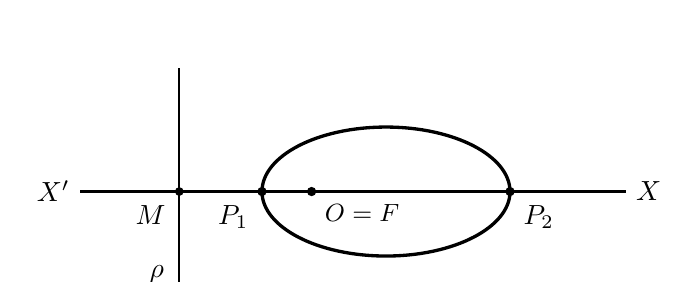
\begin{tikzpicture}[scale=1.05]
  % Directrix \rho at x = -1.6
  \draw[thick] (-1.6, -1.2) -- (-1.6, 1.5);
  \node[left=2pt] at (-1.6, -1.0) {$\rho$};

  % Horizontal line X'X
  \draw[thick] (-2.8, 0) node[left] {$X'$} -- (3.8, 0) node[right] {$X$};

  % Intersection M
  \fill (-1.6, 0) circle (1.5pt) node[below left=2pt] {$M$};

  % Ellipse: P_1 at -0.6, P_2 at 2.4, center at 0.9, x radius = 1.5, y radius = 0.78
  \draw[very thick] (0.9, 0) ellipse [x radius=1.5, y radius=0.78];

  % Points P_1, O=F, P_2
  \fill (-0.6, 0) circle (1.6pt);
  \node[below left=2pt] at (-0.6, 0) {$P_1$};

  \fill (0, 0) circle (1.6pt);
  \node[below right=1pt, font=\small] at (0.02, -0.02) {$O=F$};

  \fill (2.4, 0) circle (1.6pt);
  \node[below right=2pt] at (2.4, 0) {$P_2$};
\end{tikzpicture}
\caption*{圖 5-3}
\label{fig:b5s-5-3}
\end{figure}

\noindent
\textbf{注意}\quad $P_1$ 與 $P_2$ 一在 $OM$ 之間，一在 $O$ 的右側，而同在 $\rho$ 的右側，這一觀察正是 $\Gamma$ 為橢圓時，如圖 5-3，所應有的現象。

\paragraph*{(ii) \underline{當 $e = 1$ 時}}
在水平軸 $X'X$ 上，$\Gamma$ 只交一次且正好是線段 $OM$ 的中點。

\begin{figure}[H]
\centering
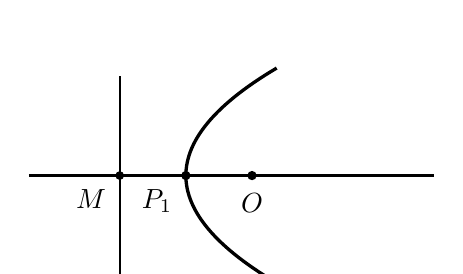
\begin{tikzpicture}[scale=1.05]
  % Directrix \rho at x = -1.6
  \draw[thick] (-1.6, -1.2) -- (-1.6, 1.2);

  % Horizontal axis X'X
  \draw[thick] (-2.7, 0) -- (2.2, 0);

  % Point M at (-1.6, 0), O at (0, 0), P_1 at (-0.8, 0)
  \fill (-1.6, 0) circle (1.5pt) node[below left=2pt] {$M$};
  \fill (-0.8, 0) circle (1.6pt) node[below left=2pt] {$P_1$};
  \fill (0, 0) circle (1.6pt) node[below=3pt] {$O$};

  % Parabola opening right with vertex at P_1(-0.8, 0)
  \draw[very thick, domain=-1.3:1.3, samples=60]
    plot ({-0.8 + 0.65*(\x)^2}, {\x});
\end{tikzpicture}
\caption*{圖 5-4}
\label{fig:b5s-5-4}
\end{figure}

\paragraph*{(iii) \underline{當 $e > 1$ 時}}
在水平軸 $X'X$ 上，$\Gamma$ 交 $X'X$ 兩次，其一仍在 $O$ 與 $M$ 之間，另一則反落到 $M$ 的左側（或 $\rho$ 的左側）。

\begin{figure}[H]
\centering
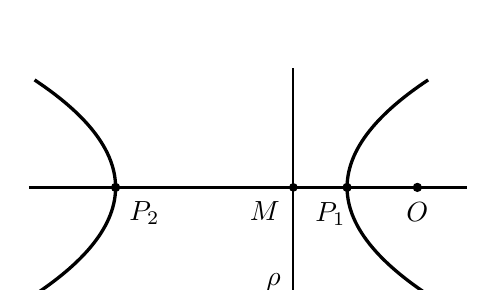
\begin{tikzpicture}[scale=1.05]
  % Directrix \rho at x = 0
  \draw[thick] (0, -1.35) -- (0, 1.45);
  \node[left=1pt] at (0, -1.15) {$\rho$};

  % Horizontal line X'X
  \draw[thick] (-3.2, 0) -- (2.1, 0);

  % Points P_2, M, P_1, O
  \fill (0, 0) circle (1.5pt) node[below left=2pt] {$M$};
  \fill (0.65, 0) circle (1.6pt);
  \node[below=2pt] at (0.45, 0) {$P_1$};
  \fill (1.5, 0) circle (1.6pt) node[below=2pt] {$O$};
  \fill (-2.15, 0) circle (1.6pt);
  \node[below right=2pt] at (-2.15, 0) {$P_2$};

  % Right branch through P_1(0.65, 0) opening right
  \draw[very thick, domain=-1.3:1.3, samples=60]
    plot ({0.65 + 0.58*(\x)^2}, {\x});

  % Left branch through P_2(-2.15, 0) opening left
  \draw[very thick, domain=-1.3:1.3, samples=60]
    plot ({-2.15 - 0.58*(\x)^2}, {\x});
\end{tikzpicture}
\caption*{圖 5-5}
\label{fig:b5s-5-5}
\end{figure}

\subsubsection*{作業 14}
一直線 $L$ 上兩點 $M$ 與 $O$，試在 $L$ 上找出滿足 $\dfrac{PO}{PM} = \dfrac{1}{3}$ 的點，描於 $L$ 上，並注意其與 $O$ 的相關位置（在 $O$ 之左側或右側？）

\subsubsection*{作業 15}
用極圖觀點驗證
\[
  \begin{cases}
    r = \dfrac{pe}{1 - e\cos\theta} \\[0.6em]
    \theta = 0
  \end{cases}
\]
有兩解 $\left(\dfrac{pe}{1-e}, 0\right)$ 與 $\left(\dfrac{pe}{1+e}, 0\right)$\phantomsection\label{note:b5s-ch1-p48-hw15}\footnote{【原書註記/校訂】：原書此處聯立條件印作「$\theta = 0$」，兩解印作「$\left(\frac{pe}{1-e}, 0\right)$ 與 $\left(\frac{pe}{1+e}, 0\right)$」，緊接解釋「換句話說第二解 $r$ 為負值其實就在 $\theta = \pi$ 的方向上」。按極平面上直線 $X'X$ 包含 $\theta = 0$ 與 $\theta = \pi$ 兩方向：當 $\theta = \pi$ 時代入極方程式得 $r = \frac{pe}{1 - e\cos\pi} = \frac{pe}{1+e}$，對應極座標為 $\left[\frac{pe}{1+e}, \pi\right]$；若改以 $\theta = 0$ 表示同一點，則其 $r$ 值為負，即 $\left[-\frac{pe}{1+e}, 0\right]$。原書於第二解漏印負號（或將角度 $\pi$ 誤印為 $0$），特此註明。}。換句話說第二解 $r$ 為負值其實就在 $\theta = \pi$ 的方向上，故 $\Gamma$ 與 $X'X$ 的兩交點分居於 $O$ 的兩側。

\subsubsection*{作業 16}
仿作業 14，直觀地看看是否 $L$ 上到 $O$ 點與到 $M$ 點等距離的點果真只有 $OM$ 中點？

\subsubsection*{作業 17}
仿\underline{作業 15} 驗證 $\Gamma$ 只交 $X'X$ 於 $OM$ 中點。

\subsubsection*{作業 18}
仿作業 14, 15 解釋 (iii) 中所述。

\subsubsection*{作業 19}
用極圖觀點證明：任一通過焦點的直線（水平線除外）與拋物線：
\[
  r = \frac{p}{1 - \cos\theta}
\]
都正好有兩個交點。

\subsubsection*{作業 20}
一通過焦點的直線與單支雙曲線的交點有幾個？從這件事你能否定義出所謂「開口」的角度，而得到拋物線的開口 $= 0$，恒小於雙曲線的開口？

\begin{discussion}\label{disc:b5s-1-5}
\underline{刻卜勒}（Kepler）第一定律說：行星繞太陽旋轉的軌道是一個以太陽為焦點的橢圓，第二定律則說：對於一固定行星，在同一時間區段內，此行星對太陽所掃出的近似扇形的面積相等，此卽為\underline{天體運動說}。從這裏你可以推論「行星運行的速度（不計其方向）在近日點時，與在遠日點時相較，那一時候快？」（作業 21）

\begin{figure}[H]
\centering
\begin{tikzpicture}[scale=1.05]
  % Ellipse centered at (0,0) with a = 2.4, b = 0.85
  % Focus (Sun) at (-1.45, 0)
  \coordinate (Sun) at (-1.45, 0);
  \coordinate (Peri) at (-2.4, 0);
  \coordinate (Aphe) at (2.4, 0);

  % Shaded sector 1 near Perihelion: from angle 152 to 205 on ellipse
  \begin{scope}
    \path[clip] (Sun) -- ({2.4*cos(152)}, {0.85*sin(152)})
      arc [start angle=152, end angle=205, x radius=2.4, y radius=0.85] -- cycle;
    \foreach \x in {-3.0, -2.9, ..., -1.0} {
      \draw[thin, gray!80!black] (\x, -1.0) -- (\x+1.2, 1.0);
    }
  \end{scope}
  \draw[thick] (Sun) -- ({2.4*cos(152)}, {0.85*sin(152)});
  \draw[thick] (Sun) -- ({2.4*cos(205)}, {0.85*sin(205)});

  % Shaded sector 2 towards Aphelion (upper right): from angle 42 to 72 on ellipse
  \begin{scope}
    \path[clip] (Sun) -- ({2.4*cos(42)}, {0.85*sin(42)})
      arc [start angle=42, end angle=72, x radius=2.4, y radius=0.85] -- cycle;
    \foreach \x in {-1.8, -1.7, ..., 2.2} {
      \draw[thin, gray!80!black] (\x, -1.0) -- (\x+1.2, 1.0);
    }
  \end{scope}
  \draw[thick] (Sun) -- ({2.4*cos(42)}, {0.85*sin(42)});
  \draw[thick] (Sun) -- ({2.4*cos(72)}, {0.85*sin(72)});

  % Ellipse outline
  \draw[very thick] (0, 0) ellipse [x radius=2.4, y radius=0.85];

  % Dots for Sun, Perihelion, Aphelion
  \fill (Sun) circle (2.5pt);
  \node[below right=1pt] at (-1.35, 0.05) {\small 太陽};

  \fill (Peri) circle (2pt);
  \node[left=4pt, align=center] at (Peri) {\small 近\\[-2pt]\small 日\\[-2pt]\small 點};

  \fill (Aphe) circle (2pt);
  \node[right=4pt] at (Aphe) {\small 遠日點};
\end{tikzpicture}
\caption*{圖 5-6}
\label{fig:b5s-5-6}
\end{figure}

但注意由於運行速度不均勻，這裏我們所說的“速度”的意義也似乎不明，這便是到了\underline{牛頓}時代所產生的前兆微分觀念。
\end{discussion}

\subsubsection*{作業 21}
上文同一行星的運行速度，離太陽越遠越快，還是越近越快？（暫且粗略判斷）

\subsubsection*{丙、決定形狀的資料}

在極方程式中，$p$ 與 $e$ 一旦決定，二次曲線的形狀也就決定，若非拋物線，則 $\{p, e\}$ 這組資料又可換成 $\{a, c\}$ 其中 $a$ 為長軸或貫軸半長，$c$ 為兩焦點間距半長，如

橢圓時，
\[
  \begin{cases}
    p = \dfrac{a}{e}(1 - e^2) = \dfrac{a^2}{c} - c \\[0.8em]
    e = \dfrac{c}{a}
  \end{cases}
\]

雙曲線時，
\[
  \begin{cases}
    p = \dfrac{a}{e}(e^2 - 1) = c - \dfrac{a^2}{c} \\[0.8em]
    e = \dfrac{c}{a}
  \end{cases}
\]

\subsubsection*{作業 22}
將上式換算式詳加驗證，並討論拋物線的情形。

\subsubsection*{丁、旋轉}

對於一個開口朝左的拋物線，我們是否稍一觀察就能利用開口朝右極方程式 \eqref{eq:b5s-1-5-1}（其中取 $e = 1$）
\[
  r = \frac{p}{1 - \cos\theta}
\]
而寫下開口朝左的極方程式？

方法由下圖 5-7

\begin{figure}[H]
\centering
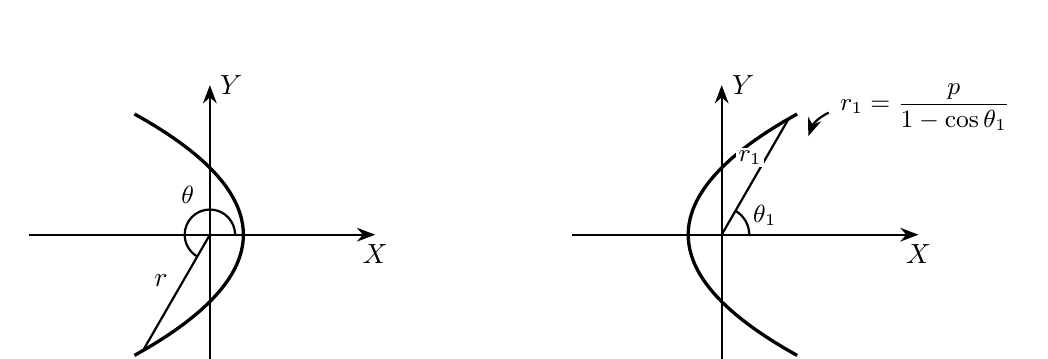
\begin{tikzpicture}[scale=1.0]
  % ==================== Left Subfigure: Opening Left ====================
  \begin{scope}[shift={(-3.5, 0)}]
    \draw[thick, -Stealth] (-2.3, 0) -- (2.1, 0) node[below] {$X$};
    \draw[thick, -Stealth] (0, -1.7) -- (0, 1.9) node[right] {$Y$};

    % Parabola opening left: r = p / (1 + cos\theta), p = 0.85
    \draw[very thick, domain=-122:122, samples=80]
      plot ({0.85/(1 + cos(\x))*cos(\x)}, {0.85/(1 + cos(\x))*sin(\x)});

    % Ray in 3rd quadrant at \theta = 240 deg
    \pgfmathsetmacro{\thL}{240}
    \pgfmathsetmacro{\rL}{0.85/(1 + cos(\thL))}
    \coordinate (PL) at ({\rL*cos(\thL)}, {\rL*sin(\thL)});
    \draw[thick] (0, 0) -- (PL);

    % Angle arc for \theta
    \draw[thick] (0.32, 0) arc (0:\thL:0.32);
    \node at (-0.28, 0.50) {\small $\theta$};

    % Label r
    \node at (-0.62, -0.58) {$r$};
  \end{scope}

  % ==================== Right Subfigure: Opening Right ====================
  \begin{scope}[shift={(3.0, 0)}]
    \draw[thick, -Stealth] (-1.9, 0) -- (2.5, 0) node[below] {$X$};
    \draw[thick, -Stealth] (0, -1.7) -- (0, 1.9) node[right] {$Y$};

    % Parabola opening right: r_1 = p / (1 - cos\theta_1), p = 0.85
    \draw[very thick, domain=58:302, samples=80]
      plot ({0.85/(1 - cos(\x))*cos(\x)}, {0.85/(1 - cos(\x))*sin(\x)});

    % Ray in 1st quadrant at \theta_1 = 60 deg
    \pgfmathsetmacro{\thR}{60}
    \pgfmathsetmacro{\rR}{0.85/(1 - cos(\thR))}
    \coordinate (PR) at ({\rR*cos(\thR)}, {\rR*sin(\thR)});
    \draw[thick] (0, 0) -- (PR);

    % Angle arc for \theta_1
    \draw[thick] (0.35, 0) arc (0:\thR:0.35);
    \node at (0.55, 0.25) {\small $\theta_1$};

    % Label r_1 cleanly inside Q1 clear of the parabola and ray
    \node[fill=white, inner sep=1pt] at (0.36, 0.98) {\small $r_1$};

    % Equation label and curved pointer to upper right branch
    \node[right] at (1.38, 1.62) {\small $r_1 = \dfrac{p}{1 - \cos\theta_1}$};
    \draw[thick, -Stealth] (1.36, 1.55) to[out=205, in=70] (1.10, 1.25);
  \end{scope}
\end{tikzpicture}
\caption*{圖 5-7}
\label{fig:b5s-5-7}
\end{figure}

討論如下：

只要左右兩圖相較，左圖之 $\theta$ 減去 $\pi$ 後記為 $\theta_1$，則相應的，
\[
  r = r_1 = \frac{p}{1 - \cos\theta_1}
\]
故
\[
  r = \frac{p}{1 - \cos(\theta - \pi)}
\]
卽
\[
  r = \frac{p}{1 + \cos\theta}
\]
\underline{一般的情形一樣}，例如一個橢圓其長軸的傾斜角為 $\theta_0$，則其極方程式由下圖 5-8

\begin{figure}[H]
\centering
\begin{tikzpicture}[scale=1.1]
  % ==================== Left Subfigure: Tilted Ellipse ====================
  \begin{scope}[shift={(-3.5, 0)}]
    \draw[thick, -Stealth] (-1.9, 0) -- (2.3, 0) node[right] {$X$};
    \draw[thick, -Stealth] (0, -1.6) -- (0, 2.15) node[above] {$Y$};

    % Major axis line at \theta_0 = 46 deg
    \draw[thick] (226:1.85) -- (46:2.45);

    % Tilted ellipse with focus at (0,0), center shifted by 0.52 along 46 deg
    % x radius = 1.55, y radius = 0.85
    \begin{scope}[rotate=46]
      \draw[very thick] (0.52, 0) ellipse [x radius=1.55, y radius=0.85];
    \end{scope}

    % Angle arc for \theta_0 (0 to 46 deg) at radius 0.36
    \draw[thick, -Stealth] (0.36, 0) arc (0:46:0.36);
    \node at (21:0.58) {\footnotesize $\theta_0$};

    % Ray at angle \theta = 104 deg (in Q2)
    \coordinate (Ptilted) at (104:1.00);
    \draw[thick] (0, 0) -- (Ptilted);

    % Angle arc for \theta (0 to 104 deg) at radius 0.82 (outside \theta_0!)
    \draw[thick, -Stealth] (0.82, 0) arc (0:104:0.82);
    \node at (75:1.02) {\small $\theta$};

    % Label r clearly inside the ellipse to the left of the ray in Q2
    \node at (130:0.48) {\small $r$};
  \end{scope}

  % ==================== Middle Rotation Arrow & Formula ====================
  \draw[thick, -Stealth] (-1.15, 0.95) to[bend left=18] node[midway, above=2pt] {\small 轉 $\theta_0$ 角} (0.95, 0.95);
  \node at (-0.10, -1.25) {$(\theta - \theta_0 = \theta_1)$};

  % ==================== Right Subfigure: Horizontal Ellipse ====================
  \begin{scope}[shift={(3.0, 0)}]
    \draw[thick, -Stealth] (-1.5, 0) -- (2.6, 0) node[right] {$X$};
    \draw[thick, -Stealth] (0, -1.6) -- (0, 2.15) node[above] {$Y$};

    % Horizontal ellipse with focus at (0,0)
    \draw[very thick] (0.52, 0) ellipse [x radius=1.55, y radius=0.85];

    % Ray at angle \theta_1 = 58 deg
    \coordinate (Phoriz) at (58:1.00);
    \draw[thick] (0, 0) -- (Phoriz);

    % Angle arc for \theta_1
    \draw[thick, -Stealth] (0.42, 0) arc (0:58:0.42);
    \node at (26:0.65) {\footnotesize $\theta_1$};

    % Label r_1 cleanly inside the ellipse between Y-axis and ray
    \node[fill=white, inner sep=0.8pt] at (70:0.62) {\footnotesize $r_1$};
  \end{scope}
\end{tikzpicture}
\caption*{圖 5-8}
\label{fig:b5s-5-8}
\end{figure}

得
\[
  r = r_1 = \frac{pe}{1 - e\cos\theta_1} = \frac{pe}{1 - e\cos(\theta - \theta_0)}\footnotemark
\]
\phantomsection\label{note:b5s-ch1-p51-eq}\footnotetext{【原書註記/校訂】：原書此式第一個分式前之等號上橫畫漏印，致外觀形似減號「$r = r_1 - \frac{pe}{1 - e\cos\theta_1}$」，按上頁同構推導應為等號「$r = r_1 = \frac{pe}{1 - e\cos\theta_1}$」，茲予校訂。}
卽
\[
  r = \frac{pe}{1 - e\cos(\theta - \theta_0)}
\]

\subsubsection*{作業 23}
設有一雙曲線，貫軸半長 $a = 1$，焦點在原點，兩焦距間半長 $c = 3$，且貫軸傾斜角為 $\dfrac{2\pi}{3}$，求其極方程式。（先求 $p, e$ 再利用旋轉）

\subsubsection*{戊、換成直角座標方程式}

今已知二次曲線的極方程式為
\begin{equation}
  r = \frac{pe}{1 - e\cos\theta} \tag{2} \label{eq:b5s-1-5-2}
\end{equation}
將它換成直角座標方程式如下：
\begin{align}
  r - re\cos\theta &= pe \nonumber \\
  r &= e(p + r\cos\theta) \nonumber \\
  r^2 &= e^2(p + r\cos\theta)^2 \tag{3} \label{eq:b5s-1-5-3}
\end{align}
表面上因平方所引入的增式 $r = -e(p + r\cos\theta)$ $\left(\text{或等價地 } r = \dfrac{-pe}{1 + e\cos\theta}\right)$，會引進增解 $\left[\dfrac{-pe}{1 + e\cos\theta}, \theta\right]$，但由於當 $\theta$ 繞半圈成 $\theta + \pi$ 時，$r$ 亦取值為 $\dfrac{pe}{1 + e\cos\theta}$，亦卽
\[
  \left[\frac{pe}{1 + e\cos\theta}, \theta + \pi\right] = \left[\frac{-pe}{1 + e\cos\theta}, \theta\right]
\]
而使 \eqref{eq:b5s-1-5-3} 式不因平方增添任何多餘的新點。（見\underline{作業 24}）則
\[
  x^2 + y^2 = e^2(p + x)^2
\]

\subsubsection*{作業 24}
一般一個
\[
  r = f(r\cos\theta, r\sin\theta)
\]
的極方程式（自為良性），經兩端平方後在極平面上所代表的軌跡不變。其道理的要點已如上文，試述其詳。

〔提示：$r = -f(r\cos\theta, r\sin\theta)$，若 $[r_1, \theta_1]$ 滿足 $r = f(r\cos\theta, r\sin\theta)$，則 $[-r_1, \theta_1 + \pi]$ 滿足 $r = -f(r\cos\theta, r\sin\theta)$〕

% =========================================================================
% 習題 I-5
% =========================================================================
\subsubsection*{習題 I-5}
\label{sec:b5s-ex1-5}

\begin{enumerate}[1.]
  \item 判別下列各極方程式在極平面上屬何種軌跡？並描畫其圖。
  \begin{multicols}{2}
  \begin{enumerate}[(a)]
    \item $r(4 - 5\cos\theta) = 7$
    \item $r(2 + \sqrt{3}\cos\theta) = 3$
    \item $r = \dfrac{1}{8(1 - \cos\theta)}$
    \item $r^2\cos 2\theta = 10$
  \end{enumerate}
  \end{multicols}

  \item
  \begin{enumerate}[(a)]
    \item 描繪極平面上
    \begin{multicols}{2}
    \begin{enumerate}[(i)]
      \item $r = \dfrac{2}{2 - \sin\theta}$
      \item $r = \dfrac{1}{1 - 2\sin\theta}$
      \item $r = \dfrac{1}{1 + \sin\theta}$
      \item $r = \dfrac{1}{1 - \sin\theta}$
    \end{enumerate}
    \end{multicols}
    之軌跡。
    \item 取原點為焦點，不過原點而平行極軸的一直線為準線，試證所得的二次曲線之極方程式為
    \[
      r = \frac{pe}{1 \pm e\sin\theta}
    \]
    並決定何時式中取正，何時取負。

    〔採用 (i) 仿本文直接導引，(ii) 旋轉取 $\dfrac{\pi}{2} - \theta$ 以代本文中 \eqref{eq:b5s-1-5-1} 式〕
  \end{enumerate}

  \item 已知某橢圓極方程式為
  \[
    r = \frac{20}{3 - 2\cos\theta}
  \]
  試求其離心率，兩焦點之位置〔以直角座標描述〕，長軸、短軸之半長，及準線位置。

  \item 極平面上一個二次曲線若知以原點為焦點，以
  \[
    2x + y + 4 = 0
  \]
  為準線，求此時二次曲線的極方程式（離心率 $e$ 已知）。

  〔提示：將本文 \eqref{eq:b5s-1-5-1} 式作一旋轉〕

  \item 設極平面上一個以原點為焦點的二次曲線上含 $P_1[2, \alpha]$, $P_2\left[4, \dfrac{\pi}{2} + \alpha\right]$, $P_3[8, \pi + \alpha]$ 三點，求其離心率。

  \item 一連結二次曲線上兩點之線段，若通過焦點 $F$ 稱為\textbf{焦弦}。試證對二次曲線
  \[
    r = \frac{pe}{1 - e\cos\theta}
  \]
  上任一焦弦 $PP'$，恒有
  \[
    \frac{1}{\overline{FP}} + \frac{1}{\overline{FP'}} = \frac{2}{pe}
  \]

  \item 適當取一極座標用以描寫“到兩定點乘積一定”之曲線〔雙紐線〕，並問這種曲線用直角座標表示時最低須為幾次？

  \item 若以有心錐線的中心為極點，軸為極軸，$e$ 為離心率，$b$ 為短軸（或共軛軸）之半長，則

  橢圓的極方程式呈 $r^2 = \dfrac{b^2}{1 - e^2\cos^2\theta}$ 型式，

  双曲線的極方程式呈 $r^2 = \dfrac{b^2}{e^2\cos^2\theta - 1}$ 型式。試驗證之。

  \item[*9.] 二次錐線 $2x^2 + 2xy + y^2 = 1$ 上之三點 $P, Q, R$ 與原點 $O$ 滿足 $\angle POQ = \angle QOR = \angle ROP$，則試導證出
  \[
    \frac{1}{\overline{OP}^2} + \frac{1}{\overline{OQ}^2} + \frac{1}{\overline{OR}^2} \quad \text{一式之值}
  \]
  與 $P, Q, R$ 三點的相對位置無關。

  \item[10.]
  \begin{enumerate}[(a)]
    \item 試化 $r = \dfrac{1}{2}\tan\theta$ 為直角座標方程式，並描其軌跡。
    \item 試化 $(x^2 + y^2)^2 = a^2(x^2 - y^2)$ 為極方程式，並描其軌跡 $[a \neq 0]$。
  \end{enumerate}
\end{enumerate}

% =========================================================================
% § I-6 極圖映射下面積的變化率
% =========================================================================
\subsection{極圖映射下面積的變化率}
\label{sec:b5s-1-6}

\begin{figure}[H]
\centering
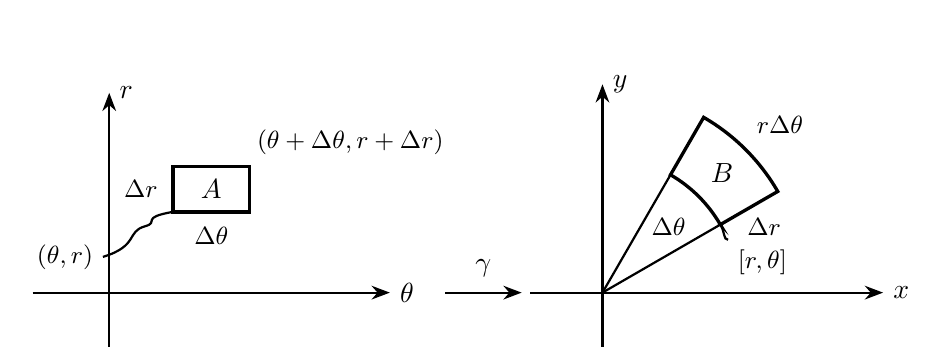
\begin{tikzpicture}[scale=1.08]
  % ==================== Left: (\theta, r)-plane ====================
  \begin{scope}[shift={(-3.5, 0)}]
    \draw[thick, -Stealth] (-0.9, 0) -- (3.3, 0) node[right] {$\theta$};
    \draw[thick, -Stealth] (0, -0.75) -- (0, 2.35) node[right] {$r$};

    % Rectangle A
    \draw[very thick] (0.75, 0.95) rectangle (1.65, 1.48);
    \node at (1.2, 1.215) {$A$};

    % Dimension labels \Delta\theta and \Delta r
    \node[below=2pt] at (1.2, 0.95) {\small $\Delta\theta$};
    \node[left=2pt] at (0.75, 1.215) {\small $\Delta r$};

    % Corner labels
    \node[above right=1pt] at (1.60, 1.48) {\small $(\theta + \Delta\theta, r + \Delta r)$};
    \node (thr) at (-0.52, 0.42) {\small $(\theta, r)$};
    % Curved leader from (\theta, r) to lower-left corner (0.75, 0.95)
    \draw[thick] (thr.east) .. controls (0.35, 0.55) and (0.20, 0.72) .. (0.42, 0.78)
      .. controls (0.60, 0.83) and (0.35, 0.88) .. (0.75, 0.95);
  \end{scope}

  % ==================== Middle Mapping Arrow \gamma ====================
  \draw[thick, -Stealth] (0.45, 0) -- node[above=2pt] {$\gamma$} (1.35, 0);

  % ==================== Right: (x, y)-plane ====================
  \begin{scope}[shift={(2.3, 0)}]
    \draw[thick, -Stealth] (-0.85, 0) -- (3.3, 0) node[right] {$x$};
    \draw[thick, -Stealth] (0, -0.75) -- (0, 2.45) node[right] {$y$};

    % Two rays at \theta_a = 30 deg and \theta_b = 60 deg
    \pgfmathsetmacro{\tha}{30}
    \pgfmathsetmacro{\thb}{60}
    \pgfmathsetmacro{\rOne}{1.60}
    \pgfmathsetmacro{\rTwo}{2.38}

    \draw[thick] (0, 0) -- (\tha:\rOne);
    \draw[thick] (0, 0) -- (\thb:\rOne);

    % Annular sector B
    \draw[very thick] (\tha:\rOne) -- (\tha:\rTwo)
      arc (\tha:\thb:\rTwo) -- (\thb:\rOne)
      arc (\thb:\tha:\rOne) -- cycle;

    \node at (45:1.99) {$B$};
    \node at (45:1.10) {\small $\Delta\theta$};
    \node at (22:2.05) {\small $\Delta r$};
    \node[above right=2pt] at (46:\rTwo) {\small $r\Delta\theta$};

    % Corner label [r, \theta] clearly below (\tha:\rOne) = (1.386, 0.80)
    \node (rth) at (1.88, 0.36) {\small $[r, \theta]$};
    \draw[thick] (rth.north west) .. controls (1.42, 0.62) and (1.44, 0.72) .. (\tha:\rOne);
  \end{scope}
\end{tikzpicture}
\caption*{圖 6-1}
\label{fig:b5s-6-1}
\end{figure}

上圖中若在 $(\theta, r)$—平面上 $\theta$ 與 $r$ 各自增加 $\Delta\theta$ 與 $\Delta r$，而考慮矩形 $A$（$A$ 之面積仍記以 $A$），另一方面經過極圖映射 $\gamma$ 後，矩形 $A$ 變成扇形靠底的一部份 $B$（$B$ 之面積仍記以 $B$）。

現在我們來計算 $B : A$ 的比值，$A$ 易知為 $A = (\Delta r)\Delta\theta$，$B$ 為大扇形與小扇形之差，故
\begin{align*}
  B &= \frac{1}{2}(r + \Delta r)^2\Delta\theta - \frac{1}{2}r^2\Delta\theta \\
    &= \frac{1}{2}(2r\Delta r + (\Delta r)^2)\Delta\theta = r\Delta r\Delta\theta + \frac{1}{2}(\Delta r)^2\Delta\theta
\end{align*}
故
\[
  \frac{B}{A} = r + \frac{1}{2}\Delta r
\]
當增量 $\Delta r \longrightarrow 0$ 時
\[
  \frac{B}{A} \longrightarrow r
\]
這表示極圖映射下面積的漲縮率隨 $r$ 值而變動。下圖 6-2 可以幫助我們了解：

\begin{figure}[H]
\centering
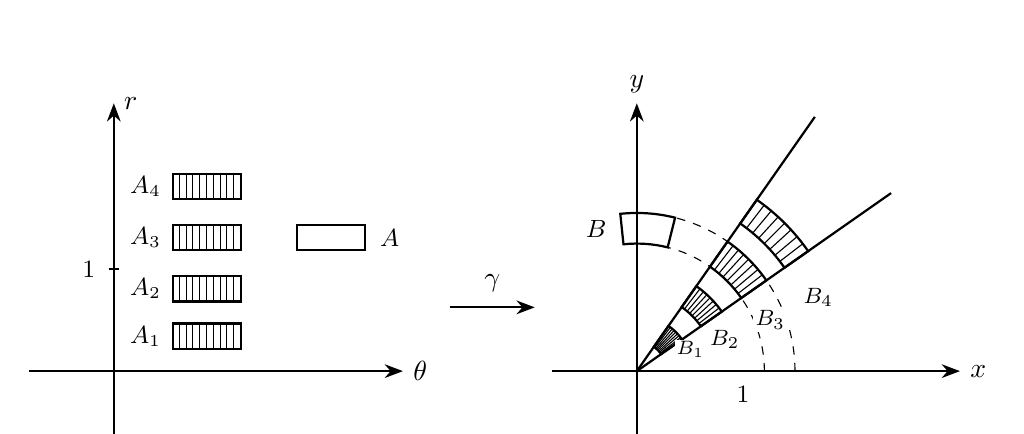
\begin{tikzpicture}[scale=1.08]
  % ==================== Left: (\theta, r)-plane ====================
  \begin{scope}[shift={(-3.7, 0)}]
    \draw[thick, -Stealth] (-1.0, 0) -- (3.4, 0) node[right] {$\theta$};
    \draw[thick, -Stealth] (0, -0.85) -- (0, 3.15) node[right] {$r$};

    % Tick mark 1 on r-axis (between A_2 and A_3)
    \draw[thick] (-0.06, 1.20) -- (0.06, 1.20);
    \node[left=2pt] at (-0.04, 1.20) {\small $1$};

    % Four congruent hatched rectangles A_1, A_2, A_3, A_4 (shifted to x in [0.70, 1.50] so labels A_i never touch the r-axis!)
    \foreach \idx/\ymin/\ymax in {1/0.26/0.56, 2/0.82/1.12, 3/1.42/1.72, 4/2.02/2.32} {
      \begin{scope}
        \path[clip] (0.70, \ymin) rectangle (1.50, \ymax);
        \foreach \x in {0.77, 0.85, ..., 1.48} {
          \draw[thin] (\x, \ymin) -- (\x, \ymax);
        }
      \end{scope}
      \draw[thick] (0.70, \ymin) rectangle (1.50, \ymax);
      \node[left=1pt] at (0.70, {0.5*(\ymin+\ymax)}) {\small $A_{\idx}$};
    }

    % Unhatched rectangle A at same height as A_3
    \draw[thick] (2.15, 1.42) rectangle (2.95, 1.72);
    \node[right=2pt] at (2.95, 1.57) {\small $A$};
  \end{scope}

  % ==================== Middle Mapping Arrow \gamma ====================
  \draw[thick, -Stealth] (0.25, 0.75) -- node[above=2pt] {$\gamma$} (1.25, 0.75);

  % ==================== Right: (x, y)-plane ====================
  \begin{scope}[shift={(2.45, 0)}]
    \draw[thick, -Stealth] (-1.0, 0) -- (3.8, 0) node[right] {$x$};
    \draw[thick, -Stealth] (0, -0.85) -- (0, 3.15) node[above] {$y$};

    % Rays at \theta_1 = 35 deg and \theta_2 = 55 deg
    \pgfmathsetmacro{\thOne}{35}
    \pgfmathsetmacro{\thTwo}{55}
    \draw[thick] (0, 0) -- (\thOne:3.65);
    \draw[thick] (0, 0) -- (\thTwo:3.65);

    % Four hatched annular sectors B_1, B_2, B_3, B_4
    \foreach \idx/\rmin/\rmax in {1/0.35/0.65, 2/0.92/1.22, 3/1.50/1.86, 4/2.12/2.46} {
      \begin{scope}
        \path[clip] (\thOne:\rmin) -- (\thOne:\rmax)
          arc (\thOne:\thTwo:\rmax) -- (\thTwo:\rmin)
          arc (\thTwo:\thOne:\rmin) -- cycle;
        \foreach \ang in {37.5, 40.0, ..., 53.5} {
          \draw[thin] (0, 0) -- (\ang:2.6);
        }
      \end{scope}
      \draw[thick] (\thOne:\rmin) -- (\thOne:\rmax)
        arc (\thOne:\thTwo:\rmax) -- (\thTwo:\rmin)
        arc (\thTwo:\thOne:\rmin) -- cycle;
    }

    % Dashed concentric arcs at r = 1.50 and r = 1.86 connecting x-axis through B_3 to B
    \draw[dashed] (0:1.50) arc (0:76:1.50);
    \draw[dashed] (0:1.86) arc (0:76:1.86);

    % Cleanly offset labels B_1, B_2, B_3, B_4 below the lower ray (35 deg) with white halo
    \node[fill=white, inner sep=0.5pt] at (22:0.68) {\scriptsize $B_1$};
    \node at (20:1.10) {\footnotesize $B_2$};
    \node[fill=white, inner sep=1pt] at (21:1.68) {\footnotesize $B_3$};
    \node at (22:2.30) {\footnotesize $B_4$};

    % Tick mark 1 on x-axis
    \node[below=2pt] at (1.25, 0) {\small $1$};

    % Unhatched annular sector B at same radius as B_3 (r in [1.50, 1.86]), angle [76, 96]
    \draw[thick] (76:1.50) -- (76:1.86)
      arc (76:96:1.86) -- (96:1.50)
      arc (96:76:1.50) -- cycle;
    \node[left=2pt] at (96:1.68) {\small $B$};
  \end{scope}
\end{tikzpicture}
\caption*{圖 6-2}
\label{fig:b5s-6-2}
\end{figure}

\noindent
\textbf{圖說：} $r$ 值增大，面積也越漲越大（如 $A_1 = A_2 = A_3 = A_4$ 而 $B_1, B_2, B_3, B_4$ 越來越大），$r$ 值相同，$\theta$ 值變動，面積漲縮率不變（如 $A = A_3$，而 $B$ 亦 $= B_3$）。
 % 第一章 極座標
% ==============================================================================
% 第二章 排列組合
% ==============================================================================
\section{排列組合}\label{sec:b5s-ch2}

\begin{center}
\begin{minipage}{0.75\textwidth}
\begin{itemize}[leftmargin=2em, itemsep=0.3em]
  \item[§ II-1] \textbf{有限集合}
  \begin{itemize}[leftmargin=2em, itemsep=0.2em]
    \item[甲、] 直\quad 積
    \item[乙、] 映\quad 射
  \end{itemize}
  \item[§ II-2] \textbf{排\quad 列}
  \begin{itemize}[leftmargin=2em, itemsep=0.2em]
    \item[甲、] 重複排列
    \item[乙、] 線性排列
    \item[丙、] 環狀排列
  \end{itemize}
  \item[§ II-3] \textbf{組\quad 合}
  \begin{itemize}[leftmargin=2em, itemsep=0.2em]
    \item[甲、] 組\quad 合
    \item[乙、] 重複組合
  \end{itemize}
  \item[§ II-4] \textbf{二項式定理}
  \begin{itemize}[leftmargin=2em, itemsep=0.2em]
    \item[甲、] 二項式定理
    \item[乙、] 多項式定理
  \end{itemize}
\end{itemize}
\end{minipage}
\end{center}

\begin{center}
$* \qquad * \qquad * \qquad * \qquad *$
\end{center}

在本章中我們介紹排列與組合的基本概念，一般規則，以及若干有系統的計數方法，雖然，排列與組合只是有限集合的理論，但是它的應用範圍都非常廣泛，這是因為不論在日常生活或科學研究方面，很多實際問題所涉及的事物都是有限的，都可以作為有限集合來討論，在下一章要講的機率就是排列與組合的一項重要應用，許多機率問題都要利用排列與組合的方法來計算。

% ==============================================================================
% § II-1 有限集合
% ==============================================================================
\subsection{有限集合}\label{sec:b5s-2-1}

因為排列與組合所討論的是有關有限集合的問題，所以我們要對有限集合有較為深入的了解，在這一節中我們首先引入集合的直積，複習映射的性質，再進一步討論有限集合到有限集合的映射。

\subsubsection*{甲、直積}

\begin{definition*}
設 $A, B$ 是兩個任意（有限的或無限的）集合，則所有元素序對 $(x, y)$，$x \in A, y \in B$，所成的集合稱為 $A$ 與 $B$ 的直積，記做 $A \times B$，也就是說
\[
A \times B = \{(x, y) \mid x \in A, y \in B\}
\]
一般地，設 $A_1, A_2, \ldots, A_n$ 是 $n$ 個任意集合，則所有元素序組 $(x_1, x_2, \ldots, x_n)$，$x_i \in A_i,\; i = 1, \ldots, n$，所成的集合稱為 $A_1, A_2, \ldots, A_n$ 的直積，記做 $A_1 \times A_2 \times \cdots \times A_n$，也就是說
\[
A_1 \times A_2 \times \cdots \times A_n = \{(x_1, x_2, \ldots, x_n) \mid x_i \in A_i,\; i = 1, \ldots, n\}
\]
\end{definition*}
由定義可知，當 $A \ne B$ 時，$A \times B \ne B \times A$，當 $B = A$ 時，$A$ 與 $B$ 的直積卽成為 $A$ 與 $A$ 本身的直積，這時我們把它簡記為 $A^2$，亦卽
\begin{align*}
A^2 = A \times A &= \{(x, y) \mid x \in A, y \in A\} \\
&= \{(x, y) \mid x, y \in A\}
\end{align*}
由此類推，$n$ 個相同集合 $A$ 的直積則簡記為 $A^n$，亦卽
\[
A^n = \underbrace{A \times \cdots \times A}_{n\text{ 個}} = \{(x_1, \ldots, x_n) \mid x_i \in A,\; i = 1, \ldots, n\}
\]

\medskip
\begin{example}\label{ex:b5s-2-1}
實數集合 $\mathbb{R}$ 與 $\mathbb{R}$ 本身的直積
\[
\mathbb{R}^2 = \mathbb{R} \times \mathbb{R} = \{(x, y) \mid x \in \mathbb{R}, y \in \mathbb{R}\}
\]
當我們考慮實數集合 $\mathbb{R}$ 與實數直線的一一對應時，則 $\mathbb{R}^2$ 卽與 $x\,y$ 平面一一對應。

同理 $\mathbb{R}^3 = \mathbb{R} \times \mathbb{R} \times \mathbb{R}$ 則與 $x\,y\,z$-空間一一對應。\hfill $\#$
\end{example}

\medskip
\begin{example}\label{ex:b5s-2-2}
設有限集合 $A=\{a_1, a_2, a_3\}$，$B=\{b_1, b_2\}$，則 $A$ 與 $B$ 的直積，
\[
A \times B = \{(a_1, b_2), (a_1, b_1), (a_2, b_1), (a_2, b_2), (a_3, b_1), (a_3, b_2)\}
\]
而 $B$ 與 $A$ 的直積為
\[
B \times A = \{(b_1, a_1), (b_1, a_2), (b_1, a_3), (b_2, a_1), (b_2, a_2), (b_2, a_3)\}
\]
顯然 $A \times B \ne B \times A$。

直積 $A \times B$ 中的元素可以依照平面上點以座標方法表示（見下面左圖），也可以用列表方式表示（下面右圖）：

\begin{figure}[H]
\centering
\begin{minipage}[c]{0.45\textwidth}
\centering
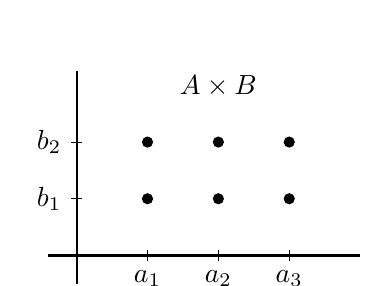
\begin{tikzpicture}[scale=0.9, >=Stealth]
  % Axes
  \draw[thick] (-0.4, 0) -- (4.0, 0);
  \draw[thick] (0, -0.4) -- (0, 2.6);
  \node[above] at (2.0, 2.1) {$A \times B$};
  
  % Ticks on x-axis
  \draw (1.0, 0.08) -- (1.0, -0.08) node[below] {$a_1$};
  \draw (2.0, 0.08) -- (2.0, -0.08) node[below] {$a_2$};
  \draw (3.0, 0.08) -- (3.0, -0.08) node[below] {$a_3$};
  
  % Ticks on y-axis
  \draw (0.08, 0.8) -- (-0.08, 0.8) node[left] {$b_1$};
  \draw (0.08, 1.6) -- (-0.08, 1.6) node[left] {$b_2$};
  
  % Points
  \foreach \x in {1.0, 2.0, 3.0} {
    \foreach \y in {0.8, 1.6} {
      \filldraw (\x, \y) circle (2pt);
    }
  }
\end{tikzpicture}
\end{minipage}
\qquad
\begin{minipage}[c]{0.45\textwidth}
\centering
\renewcommand{\arraystretch}{1.3}
\begin{tabular}{c|cc}
\diagbox[width=1.8cm, height=0.9cm]{$A$}{$B$} & $b_1$ & $b_2$ \\ \hline
$a_1$ & $(a_1, b_1)$ & $(a_1, b_2)$ \\
$a_2$ & $(a_2, b_1)$ & $(a_2, b_2)$ \\
$a_3$ & $(a_3, b_1)$ & $(a_3, b_2)$
\end{tabular}
\end{minipage}
\hfill $\#$
\end{figure}
\end{example}

現設 $A$ 為任意有限集合，我們用 $|A|$ 表示 $A$ 中所含元素個數，（在第一冊中曾用 $n(A)$ 表示，現在為避免混淆，改用 $|A|$），如果 $A$ 中共有 $m$ 個元素，則 $|A| = m$，對於直積中所含元素個數，我們有下列基本計數原則：

\medskip
\begin{theorem*}[基本計數原則]
如果 $A, B$ 是兩個有限集合，則
\begin{equation}
|A \times B| = |A| \cdot |B| \tag{1}
\end{equation}
更進一步，如果 $A_1, A_2, \ldots, A_k$ 是 $k$ 個有限集合\phantomsection\label{note:b5s-ch2-p58-k}\footnote{【原書註記/校訂】：原書此處脫漏「$k$」字，作「是個有限集合」，茲據文義校補為「是 $k$ 個有限集合」。}，則
\begin{equation}
|A_1 \times A_2 \times \cdots \times A_k| = |A_1| \cdot |A_2| \cdots\cdots |A_k| \tag{2}
\end{equation}
也就是說，直積中元素個數等於各集合中元素個數的乘積。
\end{theorem*}
\paragraph{【證明】}設 $A = \{a_1, a_2, \ldots, a_m\}$，$B = \{b_1, \ldots, b_n\}$，則
\[
A \times B = \{(a_i, b_j) \mid i = 1, \ldots, m,\; j = 1, \ldots, n\}
\]
取定 $i = 1$ 時，我們可自 $A \times B$ 中選出 $n$ 個元素
\[
(a_1, b_1), (a_1, b_2), \ldots, (a_1, b_n)
\]
同理當 $i = 2, \ldots, m$ 時，也各自得到 $n$ 個元素，將 $i$ 自 $1$ 至 $m$ 累計，卽得到總數 $m \cdot n$ 個元素，亦卽
\[
|A \times B| = |A| \cdot |B| = m \times n
\]
對於 $A_1 \times A_2 \times \cdots \times A_k$ 的情形，我們可以利用數學歸納法來證明。$k = 2$ 的情形上面已經證明成立，假設 $k - 1$ 時主張成立，卽設
\begin{equation}
|A_1 \times A_2 \times \cdots \times A_{k-1}| = |A_1| \cdot |A_2| \cdots\cdots |A_{k-1}| \tag{3}
\end{equation}
現在考慮直積 $A_1 \times A_2 \times \cdots \times A_k$，我們先要證明
\begin{equation}
|A_1 \times \cdots \times A_{k-1} \times A_k| = |(A_1 \times \cdots \times A_{k-1}) \times A_k| \tag{4}
\end{equation}
式中 $(A_1 \times \cdots \times A_{k-1}) \times A_k$ 表示集合 $A_1 \times \cdots \times A_{k-1}$ 與 $A_k$ 的直積，對於 $x_i \in A_i,\; i = 1, \ldots, k$，我們定義下列對應
\[
(x_1, \ldots, x_{k-1}, x_k) \longleftrightarrow ((x_1, \ldots, x_{k-1}), x_k)
\]
這個對應顯然為 $A_1 \times \cdots \times A_{k-1} \times A_k$ 與 $(A_1 \times \cdots \times A_{k-1}) \times A_k$ 之間的一一對應，由此可知這兩個集合中元素個數相等，亦卽 (4) 式成立，對於 $A_1 \times \cdots \times A_{k-1}$ 與 $A_k$ 兩個集合的直積，我們有
\[
|(A_1 \times \cdots \times A_{k-1}) \times A_k| = |A_1 \times \cdots \times A_{k-1}| \cdot |A_k|
\]
將 (3) 式代入上式右邊卽得所要證明的 (2) 式。\hfill $\#$

\medskip
基本計數原則也可以寫成下列方便實用的形式：

如果做一件事有 $k$ 個步驟，而第 $j$ 個步驟，可以用 $m_j$ 個方法去做，$(j = 1, \ldots, k)$，則做這件事就有
\[
m_1 m_2 \cdots m_k
\]
種方法。

例如在下面的路線圖中，由 $A_0$ 到 $A_1$ 有 3 種走法，由 $A_1$ 到 $A_2$ 有 5 種走法，由 $A_2$ 到 $A_3$ 有 7 種走法。因此由 $A_0$ 經 $A_1, A_2$ 到 $A_3$\phantomsection\label{note:b5s-ch2-p60-a3}\footnote{【原書註記/校訂】：原書此處誤植為上標「$A^3$」，茲據文義與圖 2-1 校訂為下標「$A_3$」。}共有 $3 \cdot 5 \cdot 7 = 105$ 種走法。

\begin{figure}[H]
\centering
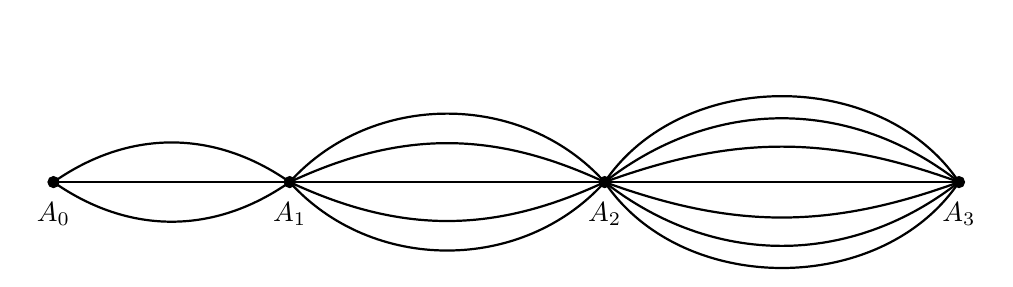
\begin{tikzpicture}[scale=1.0, >=Stealth]
  \coordinate (A0) at (0, 0);
  \coordinate (A1) at (3.0, 0);
  \coordinate (A2) at (7.0, 0);
  \coordinate (A3) at (11.5, 0);

  % Between A0 and A1: 3 paths
  \draw[thick] (A0) -- (A1);
  \draw[thick] (A0) to[out=35, in=145] (A1);
  \draw[thick] (A0) to[out=-35, in=-145] (A1);

  % Between A1 and A2: 5 paths
  \draw[thick] (A1) -- (A2);
  \draw[thick] (A1) to[out=25, in=155] (A2);
  \draw[thick] (A1) to[out=48, in=132] (A2);
  \draw[thick] (A1) to[out=-25, in=-155] (A2);
  \draw[thick] (A1) to[out=-48, in=-132] (A2);

  % Between A2 and A3: 7 paths
  \draw[thick] (A2) -- (A3);
  \draw[thick] (A2) to[out=20, in=160] (A3);
  \draw[thick] (A2) to[out=38, in=142] (A3);
  \draw[thick] (A2) to[out=56, in=124] (A3);
  \draw[thick] (A2) to[out=-20, in=-160] (A3);
  \draw[thick] (A2) to[out=-38, in=-142] (A3);
  \draw[thick] (A2) to[out=-56, in=-124] (A3);

  % Nodes
  \filldraw (A0) circle (2pt) node[below=4pt] {$A_0$};
  \filldraw (A1) circle (2pt) node[below=4pt] {$A_1$};
  \filldraw (A2) circle (2pt) node[below=4pt] {$A_2$};
  \filldraw (A3) circle (2pt) node[below=4pt] {$A_3$};
\end{tikzpicture}
\caption*{圖 2-1}
\label{fig:b5s-2-1}
\end{figure}

設有限集合 $A$ 的元素個數 $|A| = m$，考慮 $k$ 個 $A$ 的直積，由上述計數原則卽得
\begin{equation}
|A^k| = |\underbrace{A \times \cdots \times A}_{k\text{ 個}}| = \underbrace{|A| \cdots\cdots |A|}_{k\text{ 個}} = |A|^k = m^k \tag{5}
\end{equation}
當 $k = 2$ 時，我們把 $A^2$ 的子集
\[
D = \{(x, x) \mid x \in A\} \subset A^2
\]
稱為 $A^2$ 的對角線，顯然
\[
|D| = |A| = m
\]

\begin{figure}[H]
\centering
\begin{tikzpicture}[scale=1.0, >=Stealth]
  % Axes
  \draw[thick] (-0.3, 0) -- (4.8, 0) node[right=2pt] {$A$};
  \draw[thick] (0, -0.3) -- (0, 4.8) node[above=2pt] {$A$};

  % Ticks on x-axis
  \draw (0.8, 0.08) -- (0.8, -0.08) node[below=2pt] {$a_1$};
  \draw (1.6, 0.08) -- (1.6, -0.08) node[below=2pt] {$a_2$};
  \draw (3.8, 0.08) -- (3.8, -0.08) node[below=2pt] {$a_m$};

  % Ticks on y-axis
  \draw (0.08, 0.8) -- (-0.08, 0.8) node[left=2pt] {$a_1$};
  \draw (0.08, 1.6) -- (-0.08, 1.6) node[left=2pt] {$a_2$};
  \draw (0.08, 3.8) -- (-0.08, 3.8) node[left=2pt] {$a_m$};

  % Dashed lines
  % Diagonal
  \draw[thick, dashed] (0.3, 0.3) -- (4.3, 4.3);

  % Vertical dashed lines
  \draw[thick, dashed] (0.8, 0.8) -- (0.8, 3.8);
  \draw[thick, dashed] (1.6, 1.6) -- (1.6, 3.8);
  \draw[thick, dashed] (3.8, 0) -- (3.8, 3.8);

  % Horizontal dashed line
  \draw[thick, dashed] (0, 3.8) -- (3.8, 3.8);

  % Points
  \filldraw (0.8, 0.8) circle (2pt);
  \filldraw (1.6, 1.6) circle (2pt);
  \filldraw (3.8, 3.8) circle (2pt);
  \filldraw (0.8, 3.8) circle (2pt);
  \filldraw (1.6, 3.8) circle (2pt);
\end{tikzpicture}
\end{figure}

因此差集
\begin{equation}
|A^2 - D| = m^2 - m = m(m-1) \tag{6}
\end{equation}
也就是說 $A^2$ 中前後成分不相等的元素 $(x, y)$，$x \ne y$ 的個數等於 $m(m-1)$。

在一般情形，我們有下列定理：

\medskip
\begin{theorem}\label{thm:b5s-2-1}
設有限集合 $A$ 中元素個數 $|A| = m$，令 $E$ 表示 $A^k$ ($1 \le k \le m$) 中各成分互不相等的元素所成的子集，亦卽
\[
E = \{(x_1, \ldots, x_k) \mid x_1, \ldots, x_k \in A \text{ 但當 } i \ne j \text{ 時，} x_i \ne x_j\}
\]
則
\begin{equation}
|E| = \frac{m!}{(m-k)!} \tag{7}
\end{equation}
式中 $m! = m(m-1)\cdots\cdots 3 \cdot 2 \cdot 1$，$(m-k)! = (m-k)\cdots\cdots 3 \cdot 2 \cdot 1$（$m!$ 表示 $m, m-1, \ldots, 3, 2, 1$ 的連乘積，叫做 $m$ 的階乘，我們規定 $0$ 的階乘為 $0! = 1$）。
\end{theorem}
\paragraph{【證明】}
我們對於 $k$ 用數學歸納法來證明。

對於 $k = 2$ 及任意 $m \ge 2$，則 $E$ 卽等於上一段中的 $A^2 - D$，而 (6) 式為 (7) 式的特別情形：
\[
|E| = |A^2 - D| = m(m-1) = \frac{m!}{(m-2)!}
\]
假設 $k-1$ 及 $m-1$ ($m-1 \ge k-1$) 時定理成立，考慮 $k$ 及 $m$ ($m \ge k$) 的情形，設
\[
A = \{a_1, \ldots, a_m\}
\]
我們觀察 $E$ 中所有第一成分為 $a_1$ 的元素所成的集合
\[
\{(a_1, x_2, \ldots, x_k) \mid x_2, \ldots, x_k \in A,\; x_2, \ldots, x_k \text{ 皆不等於 } a_1 \text{ 且互異}\}
\]
顯然此集合中的元素個數與下列集合（令 $A' = A - \{a_1\}$）
\[
\{(x_2, \ldots, x_k) \mid x_2, \ldots, x_k \in A' \text{ 且 } x_2, \ldots, x_k \text{ 互異}\} \subset A'^{k-1}
\]
中元素個數相等，但已假設 $k-1$ 時 (7) 式成立，故後一集合中元素個數為
\[
\frac{(m-1)!}{[(m-1)-(k-1)]!} = \frac{(m-1)!}{(m-k)!}
\]
此亦為 $E$ 中第一成分為 $a_1$ 的元素個數，同理對於 $a_2, \ldots, a_m$ 各得相同個數，因此
\[
|E| = m \cdot \frac{(m-1)!}{(m-k)!} = \frac{m!}{(m-k)!} \hfill \#
\]

\medskip
\begin{example}\label{ex:b5s-2-3}
設 $A=\{1,2,3,4,5,6,7,8,9,10\}$，並令 $E$ 表示 $A^3$ 中各成分互不相等的元素所成的子集。則
\[
|E| = \frac{10!}{(10-3)!} = \frac{10!}{7!} = 10 \cdot 9 \cdot 8 = 720
\]
\end{example}

\subsubsection*{乙、映射}

設 $A, B$ 為兩個任意非空集合，則映射
\[
f : A \longrightarrow B
\]
將每一元素 $a \in A$ 映射到一個確定的元素 $b = f(a) \in B$，如果對於任意 $a_1, a_2 \in A$，$a_1 \ne a_2$，恆有 $f(a_1) \ne f(a_2)$，我們稱 $f$ 為 $A$ 到 $B$ 的\textbf{嵌射}（injection，卽一對一的映射），如果 $f(A) = B$ 成立我們則稱 $f$ 為 $A$ 到 $B$ 的\textbf{蓋射}（surjection，卽 $f$ 將 $A$ 映成 $B$），如果 $f$ 為嵌射且蓋射（一對一映成），則稱 $f$ 為\textbf{對射}（bijection）。

設 $A = B = \mathbb{R}$（實數集合），則在第一、二冊中我們已知以下諸函數均為從 $A$ 到 $B$ 的映射，且
\begin{enumerate}[label=(\roman*), topsep=2pt, itemsep=2pt]
  \item $f : x \longmapsto x^2$ 為 $A$ 到 $B$ 的映射，旣不是嵌射也不是蓋射。
  \item $f : x \longmapsto 2^x$ 為 $A$ 到 $B$ 的嵌射，但非蓋射。
  \item $f : x \longmapsto x^3 - x$ 為 $A$ 到 $B$ 的蓋射，但非嵌射。
  \item $f : x \longmapsto x^3$ 為 $A$ 到 $B$ 的對射。
\end{enumerate}
又若 $A = \mathbb{R} \times \mathbb{R}$，\quad $B = \mathbb{R} \times \mathbb{R}$，則
\[
f(x_1, x_2) = (a x_1 + b x_2, c x_1 + d x_2)
\]
為 $A$ 到 $B$ 的映射稱為線性映射（第四冊第一章）。

$f$ 若為嵌射，必為對射，其充要條件為 $ad - bc \ne 0$。

\medskip
\begin{example}\label{ex:b5s-2-4}
設 $A=\{a, b, c\}, B=\{0, 1\}$
\begin{enumerate}[label=(\roman*), topsep=2pt, itemsep=4pt]
  \item 定義映射 $f : A \longrightarrow B$
  \[
  f : a \longmapsto 0,\quad b \longmapsto 0,\quad c \longmapsto 1
  \]
  則 $f$ 為 $A$ 到 $B$ 的蓋射。
  \item 定義映射 $g : B \longrightarrow A$
  \[
  g : 0 \longmapsto a,\quad 1 \longmapsto b,
  \]
  則 $g$ 為 $B$ 到 $A$ 的嵌射。
  \item 定義映射 $h : A \longrightarrow A$；
  \[
  h : a \longmapsto b,\quad b \longmapsto c,\quad c \longmapsto a,
  \]
  則 $h$ 為 $A$ 到 $A$ 的對射。\hfill $\#$
\end{enumerate}
\end{example}

\medskip
\begin{example}\label{ex:b5s-2-5}
若 $A, B$ 皆為有限集合，設 $|A| = m$，$|B| = n$ 則由嵌射、蓋射及對射的意義可知：
\[
\left(
\begin{aligned}
&\text{若 } f \text{ 為嵌射（一對一），則 } m \le n\text{。} \\
&\text{若 } f \text{ 為蓋射（映成），則 } m \ge n\text{。} \\
&\text{若 } f \text{ 為對射（一對一映成），則 } m = n\text{。}
\end{aligned}
\right.
\]
當 $m = n$ 時，若 $f$ 為嵌射或蓋射，則顯然 $f$ 必為對射。\hfill $\#$
\end{example}

\medskip
下面我們要計算 $A$ 到 $B$ 的一般映射的個數。令 $B^A$ 表示所有自 $A$ 到 $B$ 的映射所成的集合（簡稱為 $A$ 到 $B$ 的映射集合），卽
\[
B^A = \{f \mid f \text{ 為 } A \text{ 到 } B \text{ 的映射}\}
\]
設 $A$ 為有限集合，為簡便計，我們設 $A = \{1, 2, \ldots, m\}$。若 $f \in B^A$，則 $f(i) = x_i \in B$，$i = 1, \ldots, m$，而用 $x_i$ 作成之序組，$(x_1, \ldots, x_m) \in B^m$。如此將 $B^A$ 中每一個元素，（卽一個映射）對應到 $B^m$ 中一個確定的元素，而且 $B^A$ 中不同的元素（卽不同的映射）對應到 $B^m$ 中不同的元素。這就是說，由對應
\[
f \longmapsto (f(1), \ldots, f(m)) \in B^m,\quad f \in B^A
\]
可定義出 $B^A$ 到 $B^m$ 的一個嵌射，反之對於任一 $(x_1, \ldots, x_m) \in B^m$ 我們可以由定義
\[
f(i) = x_i,\quad i = 1, \ldots, m,
\]
得到一個 $A$ 到 $B$ 的映射 $f$，而 $f \longmapsto (x_1, \ldots, x_m)$。

這表示所說的對應同時也是 $B^A$ 到 $B^m$ 的蓋射，因此為 $B^A$ 到 $B^m$ 的對射，這樣每一個 $A$ 到 $B$ 的映射都可以用 $B^m$ 中的一個元素來代表，因此在本質上我們對此二者可以不必加以區分，可將 $B^m$ 就看做 $A$ 到 $B$ 的映射集合。

由以上的討論，我們直接得到下列定理：

\medskip
\begin{theorem}\label{thm:b5s-2-2}
設 $A, B$ 為有限集合，$|A| = m$，$|B| = n$，令 $B^A$ 表示所有 $A$ 到 $B$ 的映射所成的集合，則
\begin{equation}
|B^A| = |B^m| = n^m. \tag{8}
\end{equation}
\end{theorem}

\medskip
\begin{discussion}\label{disc:b5s-2-1}
設 $A=\{1, 2, 3\}, B=\{a, b\}$，則 $|B^A| = 2^3 = 8$，實際上我們有下列 8 個映射：

\begin{center}
\renewcommand{\arraystretch}{1.2}
\begin{tabular}{r@{\quad}l@{\quad}|@{\quad}l}
\multicolumn{2}{c|}{$B^A$} & \multicolumn{1}{c}{$B^3$} \\ \hline
$f_1 :$ & $1 \longrightarrow a,\; 2 \longrightarrow a,\; 3 \longrightarrow a,$ & $f_1 \longrightarrow (a, a, a)$ \\
$f_2 :$ & $1 \longrightarrow a,\; 2 \longrightarrow a,\; 3 \longrightarrow b,$ & $f_2 \longrightarrow (a, a, b)$ \\
$f_3 :$ & $1 \longrightarrow a,\; 2 \longrightarrow b,\; 3 \longrightarrow a,$ & $f_3 \longrightarrow (a, b, a)$ \\
$f_4 :$ & $1 \longrightarrow b,\; 2 \longrightarrow a,\; 3 \longrightarrow a,$ & $f_4 \longrightarrow (b, a, a)$ \\
$f_5 :$ & $1 \longrightarrow a,\; 2 \longrightarrow b,\; 3 \longrightarrow b,$ & $f_5 \longrightarrow (a, b, b)$ \\
$f_6 :$ & $1 \longrightarrow b,\; 2 \longrightarrow a,\; 3 \longrightarrow b,$ & $f_6 \longrightarrow (b, a, b)$ \\
$f_7 :$ & $1 \longrightarrow b,\; 2 \longrightarrow b,\; 3 \longrightarrow a,$ & $f_7 \longrightarrow (b, b, a)$ \\
$f_8 :$ & $1 \longrightarrow b,\; 2 \longrightarrow b,\; 3 \longrightarrow b,$ & $f_8 \longrightarrow (b, b, b)$ \hfill $\#$
\end{tabular}
\end{center}
\end{discussion}

如果我們要進一步計算 $A$ 到 $B$ 的嵌射的個數，則應假設 $m \le n$，仍設 $A = \{1, 2, \ldots, m\}$ 及 $|B| = n$。如果 $f : A \longrightarrow B$ 是一個嵌射，則當 $i \ne j$ 時，$f(i) \ne f(j)$，因此序組
\[
(f(1), \ldots, f(m)) \in E = \{(x_1, \ldots, x_m) \mid x_1, \ldots, x_m \in B,\; x_1, \ldots, x_m \text{ 互異}\} \subset B^m
\]
由這個對應關係及定理 1 我們得到下列定理：

\medskip
\begin{theorem}\label{thm:b5s-2-3}
設 $m \le n$，$|A| = m$，$|B| = n$，則自 $A$ 到 $B$ 的所有嵌射個數等於
\[
\frac{n!}{(n-m)!}
\]
\end{theorem}

\medskip
\begin{example}\label{ex:b5s-2-6}
\begin{enumerate}[label=(\roman*), topsep=2pt, itemsep=4pt]
  \item 設 $A = \{1, 2\}$，$B = \{a, b, c, d\}$ 則 $A$ 到 $B$ 的嵌射個數等於 $4!/(4-2)! = 4!/2 = 12$，嵌射所成集合對應 $B^2$ 的子集（參考下圖）。
\[
\begin{aligned}
E = \{ &(a, b), (a, c), (a, d), \\
       &(b, a), (b, c), (b, d), \\
       &(c, a), (c, b), (c, d), \\
       &(d, a), (d, b), (d, c)\}
\end{aligned}
\]

\begin{figure}[H]
\centering
\begin{tikzpicture}[scale=1.0, >=Stealth]
  % Axes
  \draw[thick] (-0.5, 0) -- (4.8, 0) node[right=4pt] {$B$};
  \draw[thick] (0, -0.5) -- (0, 4.8) node[above=4pt] {$B$};

  % Ticks on x-axis
  \draw (1.0, 0.08) -- (1.0, -0.08) node[below=3pt] {$a$};
  \draw (2.0, 0.08) -- (2.0, -0.08) node[below=3pt] {$b$};
  \draw (3.0, 0.08) -- (3.0, -0.08) node[below=3pt] {$c$};
  \draw (4.0, 0.08) -- (4.0, -0.08) node[below=3pt] {$d$};

  % Ticks on y-axis
  \draw (0.08, 1.0) -- (-0.08, 1.0) node[left=3pt] {$a$};
  \draw (0.08, 2.0) -- (-0.08, 2.0) node[left=3pt] {$b$};
  \draw (0.08, 3.0) -- (-0.08, 3.0) node[left=3pt] {$c$};
  \draw (0.08, 4.0) -- (-0.08, 4.0) node[left=3pt] {$d$};

  % Label E
  \node[font=\large\bfseries] at (2.6, 4.8) {$E$};

  % Points in E (excluding diagonal x == y)
  \filldraw (1.0, 2.0) circle (2.2pt);
  \filldraw (1.0, 3.0) circle (2.2pt);
  \filldraw (1.0, 4.0) circle (2.2pt);

  \filldraw (2.0, 1.0) circle (2.2pt);
  \filldraw (2.0, 3.0) circle (2.2pt);
  \filldraw (2.0, 4.0) circle (2.2pt);

  \filldraw (3.0, 1.0) circle (2.2pt);
  \filldraw (3.0, 2.0) circle (2.2pt);
  \filldraw (3.0, 4.0) circle (2.2pt);

  \filldraw (4.0, 1.0) circle (2.2pt);
  \filldraw (4.0, 2.0) circle (2.2pt);
  \filldraw (4.0, 3.0) circle (2.2pt);
\end{tikzpicture}
\caption*{圖 2-2}
\label{fig:b5s-2-2}
\end{figure}

  \item 設 $A = B = \{1, 2, 3\}$，則 $A$ 到 $A$ 的嵌射個數等於 $3!/(3-3)! = 3!/0! = 3! = 6$。嵌射所成集合對應 $A^3$ 的子集
\[
E = \{(1, 2, 3), (1, 3, 2), (2, 1, 3), (2, 3, 1), (3, 1, 2), (3, 2, 1)\}
\]
\end{enumerate}
\end{example}

% ==============================================================================
% 習題 II-1
% ==============================================================================
\subsubsection*{習題 II-1}\label{sec:b5s-ex2-1}

\begin{enumerate}[label=\textbf{\arabic*.}]
  \item 某公司出品襯衫分紅、黃、藍、白、綠五種顏色；大、中、小三種尺碼。試用直積解釋，並圖示。
  \item 履歷表中需填性別、年齡、籍貫（省或院轄市），身高、體重、智識程度（大、中、小學）等，請用直積的意義說明。
  \item 智班有同學 50 位，仁班 51 位，勇班 52 位。若各班推派代表一人籌辦文藝展覽，共有幾種派法？
  \item 設某期愛國獎券發行 100 萬張，號碼自 000001 至 1000000。試問各數字互不相同的號碼有多少張？（將 1000000 看成 000000）。
  \item 設 $A = \{a, b, c\}$，$B = \{1, 2, 3, 4, 5\}$。試寫出
  \begin{enumerate}[label=(\arabic*)]
    \item 一個 $A$ 到 $B$ 的嵌射。
    \item 一個 $B$ 到 $A$ 的蓋射。
    \item 一個 $A$ 到 $A$ 的對射。
  \end{enumerate}
  \item 設集合 $A, B$ 如上題，試求
  \begin{enumerate}[label=(\arabic*)]
    \item $|A^B|$ 及 $|B^A|$。
    \item $A$ 到 $B$ 的嵌射個數。
    \item $A$ 到 $A$ 的對射個數。
    \item $B$ 到 $A$ 的蓋射個數。
  \end{enumerate}
\end{enumerate}

% =========================================================================
% §II-2 排列 (Pages 66–75)
% =========================================================================
\subsection{排列}\label{sec:b5s-2-2}
\setcounter{equation}{0}

排列的意義就是自 $n$ 件事物中，選取 $m$ 件，並排定次序，依所加的條件不同，而有各不同的型態。

\subsubsection*{甲、重複排列}

\noindent
\begin{minipage}[c]{0.56\textwidth}
\begin{example}\label{ex:b5s-2-7}
伏羲氏作八卦（見右圖），利用 \text{-{}-} 及 — 兩種符號，排成上中下三行而作成。

依映射觀點可令 $A = \{\text{上, 中, 下}\}$，
$B = \{\text{-{}-}, \text{—}\}$，$A$ 到 $B$ 的一個映射即相當於一卦，（例如上$\to$—，中$\to$\text{-{}-}，下$\to$—，即得一卦%
\begingroup\setlength{\fboxsep}{0pt}%
\tikz[baseline=-0.6ex, line width=1.0pt, line cap=butt]{
  \draw (0, 0.22) -- (0.36, 0.22);
  \draw (0, 0.08) -- (0.14, 0.08) (0.22, 0.08) -- (0.36, 0.08);
  \draw (0, -0.06) -- (0.36, -0.06);
}%
\endgroup%
）共可作出 $|B^A| = 2^3 = 8$ 卦。\hfill\#
\end{example}
\end{minipage}\hfill
\begin{minipage}[c]{0.42\textwidth}
\centering

\begin{tikzpicture}[scale=0.72]
  % Parameters
  \def\Rout{3.1}
  \def\Rmid{2.95}
  \def\Rin{1.5}
  \def\Rtaiji{1.4}

  % Outer double octagon
  \draw[line width=1.1pt] (22.5:\Rout) \foreach \a in {67.5,112.5,...,382.5} { -- (\a:\Rout) } -- cycle;
  \draw[line width=0.5pt] (22.5:\Rmid) \foreach \a in {67.5,112.5,...,382.5} { -- (\a:\Rmid) } -- cycle;

  % Radial lines dividing the 8 trigram sectors
  \foreach \a in {22.5,67.5,...,337.5} {
    \draw[line width=0.4pt] (\a:\Rin) -- (\a:\Rmid);
  }

  % Double circle around Taiji
  \draw[line width=0.5pt] (0,0) circle (\Rin);
  \draw[line width=0.8pt] (0,0) circle (\Rtaiji);

  % Taiji Yin-Yang
  \begin{scope}
    \clip (0,0) circle (\Rtaiji);
    \fill[white] (0,0) circle (\Rtaiji);
    % Yin (black): left half + bottom circle - top circle
    \fill[black] (0,\Rtaiji) arc (90:270:\Rtaiji)
      arc (-90:90:\Rtaiji/2)
      arc (270:90:\Rtaiji/2) -- cycle;
    % Eyes
    \fill[white] (0, -\Rtaiji/2) circle (\Rtaiji/6);
    \fill[black] (0, \Rtaiji/2) circle (\Rtaiji/6);
  \end{scope}

  % Trigram bars macro:
  % #1: angle, #2: inner (1=solid, 0=broken), #3: mid, #4: outer
  \newcommand{\trigram}[4]{
    \begin{scope}[rotate=#1]
      \foreach \y/\type in {1.85/#2, 2.22/#3, 2.59/#4} {
        \ifnum\type=1
          \draw[line width=3.0pt, line cap=butt] (-0.58, \y) -- (0.58, \y);
        \else
          \draw[line width=3.0pt, line cap=butt] (-0.58, \y) -- (-0.11, \y);
          \draw[line width=3.0pt, line cap=butt] (0.11, \y) -- (0.58, \y);
        \fi
      }
    \end{scope}
  }

  % 8 Trigrams (Earlier Heaven Bagua / 伏羲先天八卦)
  \trigram{0}{1}{1}{1}     % Top: 乾 ☰ (South)
  \trigram{-45}{0}{1}{1}   % Top-Right: 巽 ☴ (South-West)
  \trigram{-90}{0}{1}{0}   % Right: 坎 ☵ (West)
  \trigram{-135}{0}{0}{1}  % Bottom-Right: 艮 ☶ (North-West)
  \trigram{180}{0}{0}{0}   % Bottom: 坤 ☷ (North)
  \trigram{135}{1}{0}{0}   % Bottom-Left: 震 ☳ (North-East)
  \trigram{90}{1}{0}{1}    % Left: 離 ☲ (East)
  \trigram{45}{1}{1}{0}    % Top-Left: 兌 ☱ (South-East)
\end{tikzpicture}
\end{minipage}

\vspace{1em}
\begin{example}\label{ex:b5s-2-8}
(i) 將圍棋的黑白兩種棋子（各一缽）混在一起，每次任取一子，共取十次，依次排成一列，問共有多少可能情形？
\par\smallskip\noindent\textbf{【解】}\quad 令集合 $A = \{\text{黑}, \text{白}\}$，則任意 10 子排成一行皆可視為 $A^{10}$ 中的一個元素，因此共有 $|A^{10}| = 2^{10}$ 種可能情形。

\indent(ii) 一元硬幣有正背兩面（例如認定有梅花的為正面），投擲一次即得到正面或背面，如果連擲 10 次記錄下來，問共有多少可能結果？
\par\smallskip\noindent\textbf{【解】}\quad 這個問題在本質上與 (i) 相同，答案亦為 $2^{10}$。\hfill\#
\end{example}

\vspace{1em}
\begin{example}[摩爾斯電碼 (Morse code)]\label{ex:b5s-2-9}

摩爾斯將 26 個英文字母以 $\{\cdot, -\}$ 兩種符號編成電碼，供拍發電報之用（$\cdot$ 表示短音，$-$ 表示長音），用一個符號只能作成 2 組 $\{\cdot \text{ 及 } -\}$，用兩個符號可作成 4 組（$\cdot\cdot$, $\cdot-$, $-\cdot$ 及 $--$），用三個符號可作成 $2^3 = 8$ 組，用四個符號可作成 $2^4 = 16$ 組，因此用一至四個符號共可作成 $2 + 4 + 8 + 16 = 30$ 組，用以表示 26 個英文字母尚餘 4 個。

\begin{center}
\begin{tabular}{c@{\hspace{4em}}c@{\hspace{4em}}c}
$\begin{aligned}
a &\quad \cdot\ - \\
b &\quad -\ \cdot\ \cdot\ \cdot \\
c &\quad -\ \cdot\ -\ \cdot \\
d &\quad -\ \cdot\ \cdot \\
e &\quad \cdot \\
f &\quad \cdot\ \cdot\ -\ \cdot \\
g &\quad -\ -\ \cdot \\
h &\quad \cdot\ \cdot\ \cdot\ \cdot \\
i &\quad \cdot\ \cdot
\end{aligned}$
&
$\begin{aligned}
j &\quad \cdot\ -\ -\ - \\
k &\quad -\ \cdot\ - \\
l &\quad \cdot\ -\ \cdot\ \cdot \\
m &\quad -\ - \\
n &\quad -\ \cdot \\
o &\quad -\ -\ - \\
p &\quad \cdot\ -\ -\ \cdot \\
q &\quad -\ -\ \cdot\ - \\
r &\quad \cdot\ -\ \cdot
\end{aligned}$
&
$\begin{aligned}
s &\quad \cdot\ \cdot\ \cdot \\
t &\quad - \\
u &\quad \cdot\ \cdot\ - \\
v &\quad \cdot\ \cdot\ \cdot\ - \\
w &\quad \cdot\ -\ - \\
x &\quad -\ \cdot\ \cdot\ - \\
y &\quad -\ \cdot\ -\ - \\
z &\quad -\ -\ \cdot\ \cdot
\end{aligned}$
\end{tabular}
\end{center}
\end{example}

\vspace{1em}
\begin{discussion}\label{disc:b5s-2-2}
將 $m$ 個不同的球（可編成 1 至 $m$ 號），任意放入 $n$ 個箱子中（每箱中個數不限制），問共有多少種放置方法？
\end{discussion}
\paragraph{【解】}
每一個球可隨意放入 $n$ 個箱子中的某一個，故有 $n$ 個可能，則 $m$ 個球共有 $n^m$ 種可能放法。

\vspace{0.5em}
上面幾個都是重複排列的問題，現在給予定義如下：

\begin{definition*}
設集合 $B=\{b_1, \dots, b_n\}$，自 $B$ 中任意選出 $m$ 個元素（可以重複選取），排成一列，叫做 $n$ 中取 $m$ 的\underline{重複排列}。
\end{definition*}

若 $A = \{a_1, \dots, a_m\}$ 及 $f$ 是 $A$ 到 $B$ 的一個映射，我們把像點，$f(a_1), \dots, f(a_m)$ 依次排列，顯然得到一個 $n$ 中取 $m$ 的重複排列，反之若自 $B$ 中取 $m$ 個（可以重複）元素排成一列，依次作為 $a_1, \dots, a_m$ 的像點，則得到一個自 $A$ 到 $B$ 的映射，由此可以看出 $n$ 中取 $m$ 的重複排列與自 $A$ 到 $B$ 的映射實際上是同一件事。

由以上的討論及定義，可知下列定理成立。

\begin{theorem}\label{thm:b5s-2-4}
設 $A, B$ 為有限集合，$|A|=m$，$|B|=n$，則下列各事項在本質上具有相同意義：
\begin{enumerate}[label=\Roman*., itemsep=2pt, topsep=2pt]
  \item $n$ 中取 $m$ 的重複排列。
  \item $A$ 到 $B$ 的任意映射。
  \item $B^m$ 中的一個任意元素。
  \item $m$ 個不同的球放入 $n$ 個箱中（不限制每箱中放入球數）
\end{enumerate}
\end{theorem}

\begin{corollary*}
$n$ 中取 $m$ 的重複排列的總數為 $n^m$。
\end{corollary*}

\subsubsection*{乙、線形排列}

將一組事物排成一列叫做線形排列\phantomsection\label{note:b5s-ch2-linear-perm}\footnote{【原書註記/校訂】：原書標題及內文作「線形排列」，即現行通稱之「直線排列」或「線性排列」。}，上段中所講的重複排列就是線形排列的一種，本段中將討論不重複排列以及某些指定條件下的線形排列。

\begin{definition*}
設集合 $B=\{b_1, \dots, b_n\}$。每次自 $B$ 中任取一元素，已取者不得重複選取，連取 $m$ 次（$m \le n$）後依序排成一列，叫做 $n$ 中取 $m$ 的（不重複）排列，$n$ 中取 $m$ 的排列總數以 $P_m^n$（或 $_n P_m$，$P(n,m)$）表示。
\end{definition*}

如果我們令 $A=\{1, \dots, m\}$，則自 $B$ 中依次取 $m$ 個相異元素的排列就相當於一個自 $A$ 到 $B$ 的嵌射（一對一映射），因此依 \S 1 中的解釋也可以看作 $B^m$ 中的一個各成分互異的元素，此外如果我們仿照論例 2 的情形，將 $m$ 個不同的球放入 $n$ 個箱子，但在此處限制每箱中至多一球，那麼每一種放法就相當於一種 $n$ 中取 $m$ 的排列，因此，我們亦有下列定理。

\begin{theorem}\label{thm:b5s-2-5}
設 $A, B$ 為有限集合，$|A|=m$，$|B|=n$，($m \le n$)，則下列各事項在本質上具有相同意義。
\begin{enumerate}[label=\Roman*., itemsep=2pt, topsep=2pt]
  \item $n$ 中取 $m$ 的（不重複）排列。
  \item $A$ 到 $B$ 的一個嵌射。
  \item $B^m$ 中的一個各成分互異的元素。
  \item $m$ 個不同的球放入 $n$ 個箱中（每箱中至多放一球）
\end{enumerate}
\end{theorem}

\begin{corollary}\label{cor:b5s-2-1}
$n$ 中取 $m$ 的（不重複）排列的總數。
\begin{equation}
P_m^n = \frac{n!}{(n-m)!}, \quad 0 \le m \le n.
\end{equation}
（我們約定 $n$ 中取 0，即不取的排列總數為 1，(1) 式仍成立），這個系理可由定理 1 直接推得。
\end{corollary}

\begin{corollary}\label{cor:b5s-2-2}
如將 $n$ 個不同事物依任意次序排成一列，則各種不同排列的總數為 $n!$。
\end{corollary}

\indent 系理 2 是系理 1 中 $m=n$ 的特別情形，亦即 $n$ 中取 $n$ 的排列，所以總數為
\[
P_n^n = \frac{n!}{(n-n)!} = \frac{n!}{0!} = n!
\]

\begin{discussion}\label{disc:b5s-2-3}
趙一、錢二、孫三、李四、周五等五人組成一理事會，現欲推選理事長一人，秘書一人（理事長不能兼秘書），問共有多少可能結果？
\end{discussion}
\paragraph{【解】}
這個問題為 5 中取 2 的排列，故總數為
\[
P_2^5 = \frac{5!}{(5-2)!} = \frac{5!}{3!} = 5 \cdot 4 = 20.
\]

這一類問題也可以用下列樹枝圖來表示和計算，最下面的總數，即為答案：

\begin{center}
\begin{tikzpicture}[xscale=0.80, yscale=1.05]
  \coordinate (root) at (6.0, 2.1);
  \node[left] at (-0.4, 1.15) {理事長};
  \coordinate (Z) at (1.0, 1.15);
  \coordinate (Q) at (3.5, 1.15);
  \coordinate (S) at (6.0, 1.15);
  \coordinate (L) at (8.5, 1.15);
  \coordinate (W) at (11.0, 1.15);

  \node (nZ) at (Z) {趙};
  \node (nQ) at (Q) {錢};
  \node (nS) at (S) {孫};
  \node (nL) at (L) {李};
  \node (nW) at (W) {周};

  \draw[semithick] (root) -- (nZ);
  \draw[semithick] (root) -- (nQ);
  \draw[semithick] (root) -- (nS);
  \draw[semithick] (root) -- (nL);
  \draw[semithick] (root) -- (nW);

  \node[left] at (-0.4, -0.35) {秘\quad 書};

  \foreach \name/\x in {錢/0.25, 孫/0.75, 李/1.25, 周/1.75} {
    \node[inner sep=1.5pt] (leaf) at (\x, -0.35) {\footnotesize \name};
    \draw[semithick] (nZ.south) -- (leaf.north);
  }
  \foreach \name/\x in {趙/2.75, 孫/3.25, 李/3.75, 周/4.25} {
    \node[inner sep=1.5pt] (leaf) at (\x, -0.35) {\footnotesize \name};
    \draw[semithick] (nQ.south) -- (leaf.north);
  }
  \foreach \name/\x in {趙/5.25, 錢/5.75, 李/6.25, 周/6.75} {
    \node[inner sep=1.5pt] (leaf) at (\x, -0.35) {\footnotesize \name};
    \draw[semithick] (nS.south) -- (leaf.north);
  }
  \foreach \name/\x in {趙/7.75, 錢/8.25, 孫/8.75, 周/9.25} {
    \node[inner sep=1.5pt] (leaf) at (\x, -0.35) {\footnotesize \name};
    \draw[semithick] (nL.south) -- (leaf.north);
  }
  \foreach \name/\x in {趙/10.25, 錢/10.75, 孫/11.25, 李/11.75} {
    \node[inner sep=1.5pt] (leaf) at (\x, -0.35) {\footnotesize \name};
    \draw[semithick] (nW.south) -- (leaf.north);
  }
\end{tikzpicture}

\vspace{0.3em}
\makebox[\linewidth][c]{圖 2-3}\llap{\#}
\end{center}

\vspace{1em}
\noindent
\begin{minipage}[c]{0.68\textwidth}
\begin{example}\label{ex:b5s-2-10}
(i) 垃圾車從社區的入口處 $A$ 進來，從出口處 $B$ 出去，要走過所有巷路（$a$ 圖），但走過的路不該再走，試問有幾種走法？
\par\smallskip\noindent\textbf{【解】}\quad 在 $A$ 處要選擇三條巷路中的一條，至 $B$ 處則要選另二條中的一條，所以這是 3 中取 2 的排列，答案為
\[
P_2^3 = \frac{3!}{(3-2)!} = \frac{3!}{1!} = 3! = 6
\]

\indent(ii) 問題同上，但社區巷路如 $b$ 圖。
\par\smallskip\noindent\textbf{【解】}\quad $C, D$ 之間有三條路，由 (i) 可知 $C, D$ 之間有 6 種走法，因此共有
\[
6 \cdot 6 = 36 \text{ 種走法。}
\]
\end{example}
\end{minipage}\hfill
\begin{minipage}[c]{0.30\textwidth}
\centering
\begin{tikzpicture}[>=Stealth, scale=0.72]
  % (a)
  \begin{scope}[shift={(0,3.9)}]
    \node[left=6pt] at (-1.1, 0) {$(a)$};
    \draw[thick] (-1.1, -0.9) rectangle (1.1, 0.9);
    \draw[thick] (0, -0.9) -- (0, 0.9);
    \draw[->, thick] (0, 1.45) -- (0, 0.9);
    \node[above left] at (0, 0.9) {$A$};
    \draw[->, thick] (0, -0.9) -- (0, -1.45);
    \node[below left] at (0, -0.9) {$B$};
  \end{scope}

  % (b)
  \begin{scope}[shift={(0,0)}]
    \node[left=6pt] at (-1.4, 0) {$(b)$};
    \draw[thick] (-1.4, -1.2) rectangle (1.4, 1.2);
    \draw[thick] (-0.75, -0.6) rectangle (0.75, 0.6);
    \draw[thick] (0, -1.2) -- (0, 1.2);
    \draw[->, thick] (0, 1.75) -- (0, 1.2);
    \node[above left] at (0, 1.2) {$A$};
    \node[above left] at (0, 0.6) {$C$};
    \node[below left] at (0, -0.6) {$D$};
    \draw[->, thick] (0, -1.2) -- (0, -1.75);
    \node[below left] at (0, -1.2) {$B$};
  \end{scope}
  \node[below=8pt] at (0, -1.75) {\small 圖 2-4};
\end{tikzpicture}
\end{minipage}

\vspace{1em}
\begin{example}\label{ex:b5s-2-11}
(i) 男老師 4 人及女老師 2 人排成一列，合攝團體照，女老師 2 人願相鄰排立，問共有多少種排法？
\par\smallskip\noindent\textbf{【解】}\quad 因女老師 2 人要相鄰排立，暫將女老師 2 人視為 1 人，成為 5 人的排列問題，有 $P_5^5 = 5!$ 種方法，又女老師 2 人之間有 $P_2^2 = 2!$ 種排立方法，故共有 $5! \, 2! = 120 \cdot 2 = 240$ 種排立方法。

\indent(ii) 跳土風舞時，男女學生各 5 人間隔排成一列，問共有幾種排法？
\par\smallskip\noindent\textbf{【解】}\quad 因為間隔排列，設女生排在 $1, 3, 5, 7, 9$ 位，有 $P_5^5 = 5!$ 種排法，男生排在 $2, 4, 6, 8, 10$ 位，亦有 $5!$ 種排法。因此女生排頭時共有 $5! \cdot 5!$ 種排法，同理，男生為排頭時亦有 $5! \cdot 5!$ 種排法，兩者合有 $2 \cdot 5! \cdot 5!$ 種排法。
\end{example}

\vspace{1em}
\noindent
\begin{minipage}[t]{0.66\textwidth}
\begin{discussion}\label{disc:b5s-2-4}
用 7 種顏色填入右圖的小丑面具，相鄰的部分不得同色，問共有幾種塗法？
\end{discussion}
\paragraph{【解】}
先將面具各部分適當編定次序，再依次考慮各部分的可能塗法。設編定次序如圖中所示，

\indent 則 1 中有 7 種塗法

\indent 2 與 1 相鄰，故有 6 種塗法

\indent 3 與 1, 2 相鄰，有 5 種塗法，(因 1, 2 顏色不同)

\indent 4 與 1, 2, 3 相鄰，有 4 種塗法，(因 1, 2, 3 顏色不同)

\indent 5 只與 3 相鄰，有 6 種塗法，

\indent 6 只與 4 相鄰，有 6 種塗法，

因此共有 $7 \cdot 6 \cdot 5 \cdot 4 \cdot 6 \cdot 6 = 7 \cdot 6^3 \cdot 5 \cdot 4$ 種塗法。\hfill\#
\end{minipage}\hfill
\begin{minipage}[t]{0.32\textwidth}
\centering
\vspace{1em}
\begin{tikzpicture}[scale=0.95]
  \draw[thick] (0,0) circle (1.8);
  \draw[thick] (-1.8, 0) -- (1.8, 0);
  \draw[thick] (0, 0) -- (0, 1.8);
  % mouth
  \draw[thick] (-0.8, 0) arc (180:360:0.8);
  \node at (0, -0.45) {$1$};
  \node at (0, -1.2) {$2$};
  % eyes
  \draw[thick] (-0.8, 0.85) circle (0.45);
  \node at (-0.8, 0.85) {$5$};
  \draw[thick] (0.8, 0.85) circle (0.45);
  \node at (0.8, 0.85) {$6$};
  \node at (-0.25, 0.25) {$3$};
  \node at (0.25, 0.25) {$4$};
  \node[below=8pt] at (0, -1.8) {\small 圖 2-5};
\end{tikzpicture}
\end{minipage}

\vspace{0.5em}
\paragraph{注意：}
如果次序編排不適當，例如先塗兩眼部分，則討論較為複雜。

\vspace{1em}
\begin{discussion}\label{disc:b5s-2-5}
將「庭院深深深幾許」七個字任意排列，問共有幾種排法。
\end{discussion}
\paragraph{【解】}
由系理 2 可知七個不同的字的排列總數為 $7!$，但在此題三個深字相同，這三個字之間任意交換不改變排列形狀，三個字的排列總數為 $3!$，因此答案為 $7!/3!$。

\vspace{1em}
\begin{discussion}\label{disc:b5s-2-6}
某校招入高三插班生 10 人，擬分配智班 2 人，仁班 5 人，勇班 3 人，問共有幾種分配方法？
\end{discussion}
\paragraph{【解】}
先考慮 10 人的排列，總數為 $10!$ 種，對於每一排列，將 1, 2 位分入智班，第 $3 - 7$ 位分入仁班，第 $8 - 10$ 位分入勇班，可是如果我們將分入智班 2 人的排列次序相互改變，分配結果不變，綜合考慮智、仁、勇三班的情形，可知每一種分配，結果實際上皆由 $2! \cdot 5! \cdot 3!$ 種排列得到，因此共有 $10! / (2! \cdot 5! \cdot 3!)$ 種分配方法。\hfill\#

仿照論例 5 及 6 的討論，我們不難推出下列定理。

\begin{theorem}\label{thm:b5s-2-6}
設 $m \ge n$，將 $m$ 個不同的球放入 $n$ 個箱子，規定第 $i$ 個箱子中放 $m_i$ 個（$i=1, \dots, n$；$m_1 + \dots + m_n = m$）。則共有
\begin{equation}
\frac{m!}{m_1! \cdots m_n!}
\end{equation}
種分配方法，這也就是 $n$ 類物件，各有 $m_k$ 個，$k=1, \dots, n$，共 $m$ 個物件的排列總數。
\end{theorem}

\begin{discussion}\label{disc:b5s-2-7}
(i) 設 $A = \{1, \dots, 10\}$，$B = \{a, b, c\}$，問 $A$ 到 $B$ 的映射中取 $a$ 值 2 次，取 $b$ 值 5 次，取 $c$ 值 3 次的蓋射有幾個？
\par\smallskip\noindent\textbf{【解】}\quad 這個問題在本質上與論例 6 相同，答案為
\[
\frac{10!}{2! \, 5! \, 3!}
\]

\indent(ii) 取圍棋白子 5 個，黑子 5 點\phantomsection\label{note:b5s-ch2-p72-go-stones}\footnote{【原書註記/校訂】：原書第 72 頁【論例 7】(ii) 印作「白子 5 個，黑子 5 點」，其中「5 點」即「5 個（顆）」之意，此處保留原書用字並附註說明。}，任意排列，問總數多少？
\par\smallskip\noindent\textbf{【解】}\quad 考慮 $A = \{1, \dots, 10\}$ 到 $B = \{\text{黑}, \text{白}\}$ 的映射，則映射到黑子，白子各 5 次的蓋射個數。\phantomsection\label{note:b5s-ch2-p72-surjection-period}\footnote{【原書註記/校訂】：原書「則映射到黑子，白子各 5 次的蓋射個數。」句末印有句號，其下緊接計算式 $\frac{10!}{5!\,5!}$ 及「即為所求答案。」}
\[
\frac{10!}{5! \, 5!}
\]
即為所求答案。

\indent(iii) 設由 $A$ 到 $B$ 的街道如下圖，試問如不繞遠路（最短路線）共有幾種走法？

\begin{center}
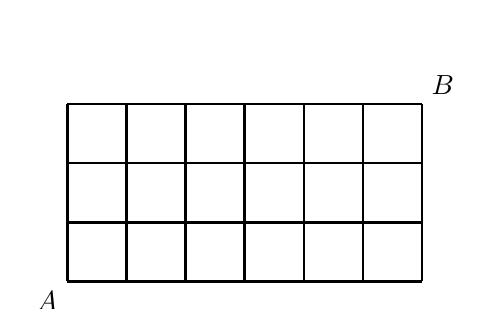
\begin{tikzpicture}[scale=0.75]
  \draw[thick] (0,0) grid (6,3);
  \node[below left] at (0,0) {$A$};
  \node[above right] at (6,3) {$B$};
\end{tikzpicture}

\vspace{0.3em}
圖 2-6
\end{center}
\par\smallskip\noindent\textbf{【解】}\quad 設向東走一小段（一個街口到次一街口）用 $E$ 表示，向北走一小段用 $N$ 表示，則每一種走法都是由 6 個 $E$ 及 3 個 $N$ 排列而成，例如 EEEEEENNN，因此由 (2) 式即得答案為 $9! / (6! \, 3!)$。\hfill\#
\end{discussion}

\subsubsection*{丙、環狀排列}

以上所講的都是線形排列，現在要講的是另一形狀的排列，我們將 $m$ 個不同的事物排成環狀，叫做環狀排列，在這裏我們只考慮這 $m$ 個事物的相關位置，而不計較各事物所在之實際位置，也就是說，如果將排成的環形任意轉動，所得到的結果仍表示同一環形排列，例如趙、錢、孫、李四人坐一圓桌，下列各圖形都表示同一環狀排列：

\begin{center}
\begin{tikzpicture}[scale=0.78]
  \foreach \cx/\top/\left/\bot/\right in {
    0/趙/錢/孫/李,
    4.1/李/趙/錢/孫,
    8.2/孫/李/趙/錢,
    12.3/錢/孫/李/趙
  } {
    \draw[thick] (\cx, 0) circle (1.1);
    \node[above] at (\cx, 1.1) {\top};
    \node[left] at (\cx - 1.1, 0) {\left};
    \node[below] at (\cx, -1.1) {\bot};
    \node[right] at (\cx + 1.1, 0) {\right};
  }
\end{tikzpicture}

\vspace{0.3em}
圖 2-7
\end{center}

\begin{example}\label{ex:b5s-2-12}
若趙、錢、孫、李四人共坐一圓桌，問共有幾種坐法？
\end{example}
\paragraph{【解】}
因為環狀排列只考慮相關位置，我們可以假想趙已坐定某一位置，再將錢、孫、李三位排入其餘三個位子，此時成為 3 中取 3 的線形排列問題，共有 $3!$ 種坐法，這也就是原來問題的答案。\hfill\#

這個問題我們也可以用另一種想法，先把環形看作線形，則 4 中取 4 的線形排列總數為 $P_4^4 = 4!$，此時每 4 種線形排列作成同一種環狀排列，例如（趙、錢、孫、李），（錢、孫、李、趙），（孫、李、趙、錢），（李、趙、錢、孫）四種排列作成同一個環狀排列（如前面圖所示），因此環狀排列總數為 $\dfrac{4!}{4} = 3!$。

由這個例子可知，對於一般情形我們也有下列結果：$m$ 個不同事物的環狀排列總數為
\begin{equation}
\frac{P_m^m}{m} = (m-1)!
\end{equation}
更進一步，如果我們考慮自 $n$ 個不同事物中任取 $m$ 個（不重複）事物的環狀排列，則總數為
\begin{equation}
\frac{P_m^n}{m} = \frac{1}{m} \frac{n!}{(n-m)!}
\end{equation}
換句話說，用 $m$ 去除線形排列總數就得到環狀排列總數，例如在例 14 (ii)\phantomsection\label{note:b5s-ch2-p74-ex14}\footnote{【原書註記/校訂】：原書此處印作「例如在例 14 (ii) 中」，然前文第 70 頁土風舞男女學生間隔排成一列之題目實為〔例 11〕(ii)，此處係原書編號錯參，特此註明。}中跳土風舞時，男女學生各 5 人間隔排成一列的線形排列總數為 $2 \cdot 5! \cdot 5!$，如改為間隔的環狀排列，則總數為 $\dfrac{2 \cdot 5! \cdot 5!}{10} = 4! \, 5!$。這個問題我們也可以用第一種解法，先將男生 5 人作成環狀排列，由 (3) 式有 $(5-1)! = 4!$ 種排法，再將女生 5 人間隔插入，有 $P_5^5 = 5!$ 種排法，因此共有 $4! \cdot 5!$ 種排法，答案相同。

\begin{example}\label{ex:b5s-2-13}
將 20 粒顏色不同的珠子串成手鐲，共有幾種串法？
\end{example}
\paragraph{【解】}
20 中取 20 的環狀排列總數為 $(20-1)! = 19!$

但如依照一種環狀排列串好一串後，翻轉一次就表示另一反方向的環狀排列實際上表示同一種串法，因此共有 $\dfrac{19!}{2}$ 種串法。\hfill\#

\subsubsection*{習題 II-2}

\begin{enumerate}[label=\arabic*., topsep=4pt, itemsep=6pt]
  \item 某大學聯招甲組有 108 個志願，若班上 50 位同學均考甲組，所填第一志願共有多少種可能情形？
  \item 某線鐵路有 21 個站，需印製多少種車票？
  \item
  \begin{enumerate}[label=(\arabic*), topsep=2pt, itemsep=2pt]
    \item 將 100 個不同的球放入藍、白、紅三個箱中，共有多少可能放法？
    \item 試將 (1) 的問題用映射說明。
  \end{enumerate}
  \item 某次球賽共有 7 隊參加，比賽完畢排定名次，共有多少種可能情形？（設沒有相同名次）。
  \item 11 人組成的理事會中欲推選理事長、秘書、財務各一人（皆不能兼任），推選結果共有多少可能情形？
  \item
  \begin{minipage}[t]{0.68\linewidth}
  某社區巷道如右圖，\footnotemark 早晨派報時由 $A$ 點進入，$B$ 點離去，需走過每條巷道，但不願重複走過同一條路，問共有幾種走法？
  \end{minipage}\hfill
  \begin{minipage}[t]{0.30\linewidth}
  \centering
  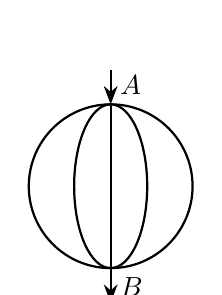
\begin{tikzpicture}[>=Stealth, scale=0.8]
    \draw[thick] (0,0) circle (1.3);
    \draw[thick] (0,0) ellipse (0.58 and 1.3);
    \draw[thick] (0,-1.3) -- (0,1.3);
    \draw[->, thick] (0, 1.85) -- (0, 1.3);
    \node[above right] at (0, 1.3) {$A$};
    \draw[->, thick] (0, -1.3) -- (0, -1.85);
    \node[below right] at (0, -1.3) {$B$};
  \end{tikzpicture}
  \end{minipage}%
  \phantomsection\label{note:b5s-ch2-p75-q6-quote}\footnotetext{【原書註記/校訂】：原書第 75 頁第 6 題「如右圖」之後印有一孤立單引號「‘」，疑為贅印或排版鉛字殘痕，此處予以刪正並附註說明。}

  \item
  \begin{minipage}[t]{0.50\linewidth}
  小明有 12 色臘筆\footnotemark，要將右邊的圖著色，相鄰的部分不得同色，共有幾種可能著法？
  \end{minipage}\hfill
  \begin{minipage}[t]{0.48\linewidth}
  \centering
  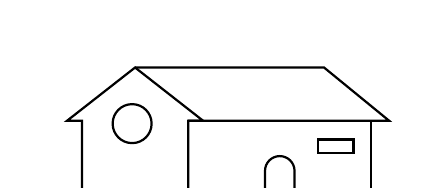
\begin{tikzpicture}[scale=0.75]
    % Ground line
    \draw[thick] (-0.6, 0) -- (6.0, 0);

    % Left front facade (with gable)
    \draw[thick] (0.3, 0) -- (0.3, 1.3) -- (0.05, 1.3) -- (1.2, 2.2) -- (2.35, 1.3) -- (2.1, 1.3) -- (2.1, 0);

    % Circular window on front gable
    \draw[thick] (1.15, 1.25) circle (0.33);

    % Right wing roof (trapezoid)
    \draw[thick] (1.2, 2.2) -- (4.4, 2.2) -- (5.5, 1.3) -- (2.1, 1.3);

    % Right wing wall
    \draw[thick] (5.2, 1.3) -- (5.2, 0);

    % Arched door on right wall
    \draw[thick] (3.4, 0) -- (3.4, 0.45) arc (180:0:0.25) -- (3.9, 0);

    % Window on right wall
    \draw[thick] (4.3, 0.75) rectangle (4.9, 0.98);
  \end{tikzpicture}
  \end{minipage}%
  \phantomsection\label{note:b5s-ch2-p75-q7-crayon}\footnotetext{【原書註記/校訂】：原書作「12 色臘筆」，「臘」通「蠟」，即蠟筆。}

  \item 跳土風舞時，男生 20 人，女生 16 人排成一長列，但女生不得相鄰，共有幾種可能排法？
\end{enumerate}

% ==============================================================================
% § II-3 組合
% ==============================================================================
\subsection{組合}\label{sec:b5s-2-3}

\subsubsection*{甲、組合}

\begin{definition*}
設 $B$ 為有限集合，$|B| = n$，對於每個自然數 $m \le n$，自 $B$ 中任取 $m$ 個不同元素作為一組（不考慮順序），叫做 $n$ 中取 $m$ 的組合。$n$ 中取 $m$ 的組合總數用 $\binom{n}{m}$ 或 $C_m^n$（或 ${}_nC_m, C(n, m)$）表示。我們約定 $n$ 中取 0，即不取，的組合總數為 1。
\end{definition*}

因為 $m$ 個不同元素的排列總數為 $P_m^m = m!$，所以在 $n$ 中取 $m$ 的一個（不重複）線形排列中，將次序變動，即可作出 $m!$ 個排列，換句話說，每 $m!$ 個排列由同一組 $m$ 個元素所作成，如不計較次序時，即為同一個 $n$ 中取 $m$ 的組合，因此我們有下列重要定理：

\medskip
\begin{theorem}\label{thm:b5s-2-7}
$n$ 中取 $m$ 的組合總數
\begin{equation}
C_m^n = P_m^n / P_m^m = \frac{n!}{(n - m)!\, m!}, \quad 0 \le m \le n. \tag{1}
\end{equation}
\end{theorem}
有了這個定理，我們可以直接計算組合總數，\hfill $\#$

\medskip
\noindent 例如\phantomsection\label{note:b5s-ch2-p75-eq}\footnote{【原書註記/校訂】：原書此處印為「$C_2^5 ==$」，多出一個等號，茲更正為「$C_2^5 =$」。}
\[
C_2^5 = \frac{5!}{(5 - 2)!\, 2!} = \frac{5!}{3!\, 2!} = \frac{5 \cdot 4}{2} = 10
\]
\[
C_5^5 = C_0^5 = 1
\]
前節中的若干重複排列問題也可以用組合方法來解，例如在論例 6 中插班生 10 人分入智、仁、勇三班的問題，我們先自 10 中取 2 分入智班，總數為 $C_2^{10}$，再在其餘 8 人中取 5 分入仁班，總數為 $C_5^8$，最後 3 人則分入勇班，因此共有
\[
C_2^{10} \cdot C_5^8 = \frac{10!}{(10 - 2)!\, 2!} \cdot \frac{8!}{(8 - 5)!\, 5!} = \frac{10!}{2!\, 5!\, 3!}
\]
種分配方法，在論例 7 (iii) 中的走法問題，自 $A$ 到 $B$ 共走九小段，向東 6\phantomsection\label{note:b5s-ch2-p76-east6}\footnote{【原書註記/校訂】：原書印作「向東段及向北 3 段」，漏印「6」，茲據前文「共走九小段」及後文「考慮那 6 段向東走」校訂補正為「向東 6 段及向北 3 段」。} 段及向北 3 段，我們只要考慮那 6 段向東走，就成為 9 中取 6 的組合問題，因此走法總數為
\[
C_6^9 = \frac{9!}{(9 - 6)!\, 6!} = \frac{9!}{3!\, 6!}
\]
由 (1) 式的形狀，我們顯然有下列關係：

\medskip
\begin{corollary*}
對於 $0 \le m \le n$，下列關係成立：
\begin{equation}
\binom{n}{m} = \binom{n}{n - m} \quad (\text{即 } C_m^n = C_{n-m}^n) \tag{2}
\end{equation}
\end{corollary*}

設 $B = \{b_1, b_2, \ldots, b_n\}$，由 $B$ 中任取 $m$ 個不同元素構成 $B$ 的一個子集，就是一個 $n$ 中取 $m$ 的組合，如果令 $C = \{0, 1\}$，考慮 $B$ 到 $C$ 的映射。恰好將 $B$ 中 $m$ 個元素對應到 1 的映射實際上也是一個 $n$ 中取 $m$ 的組合，此外如將 $m$ 個相同的球，放入 $n$ 個不同的箱子，但每箱至多一個，這也與 $n$ 中取 $m$ 的組合有同樣意義，總結這一段的討論我們寫成下列定理。

\medskip
\begin{theorem}\label{thm:b5s-2-8}
設 $0 \le m \le n$，有限集合 $B$ 中元素個數為 $|B| = n$\phantomsection\label{note:b5s-ch2-p76-thm8-dots}\footnote{【原書註記/校訂】：原書作「$|B| = n$，… 及 $C = \{0, 1\}$」，此處「…」為原書原文，疑為承接前段定義或排版留存之省略號。}，\dots 及 $C = \{0, 1\}$，則下列各事項在本質上具有相同的意義：
\begin{enumerate}[label=(\roman*), topsep=2pt, itemsep=4pt]
  \item $n$ 中取 $m$ 的組合。
  \item $B$ 中含 $m$ 個元素的子集。
  \item $B$ 到 $C$ 的映射，恰好將 $B$ 中 $m$ 個元素對應到 1。
  \item 將 $m$ 個相同的球放入 $n$ 個不同的箱子，但每箱至多一個。\hfill $\#$
\end{enumerate}
\end{theorem}

由 §II-1 定理 2 我們知道 $B$ 到 $C$ 的映射總數為 $|C^B| = |C|^n = 2^n$\phantomsection\label{note:b5s-ch2-p77-cb}\footnote{【原書註記/校訂】：原書此處印作「$|C^B| = |C^n| = 2^n \mid$」，其中「$|C^n|$」應為「$|C|^n$」（映射集合之勢），末尾之豎線「$\mid$」疑為標點或排版雜點，茲補註說明。}，根據每個映射可取出一個 $B$ 的子集，即對應到 1 的各元素所成的子集，根據恆等於 0 的映射一個元素都不取，即得到空集合 $\phi$，這樣不難看出 $B$ 中所有子集（空集合在內）的總數就等於 $B$ 到 $C$ 的映射總數，我們將 $B$ 的所有子集構成的集合用 $\mathscr{P}(B)$ 表示，亦即
\[
\mathscr{P}(B) = \{X \mid X \subset B\}
\]
我們有
\phantomsection\label{note:b5s-ch2-p77-pn}
\begin{equation}
|\mathscr{P}(B)| = |C^n| = 2^n \tag{3}\footnotemark
\end{equation}
\footnotetext{【原書註記/校訂】：原書式 (3) 印刷為「$|\mathscr{P}(B)| = |C^n| = 2^n$」，若視映射集合為笛卡兒積 $C^n = C \times \cdots \times C$，其勢記為 $|C^n|$；亦即 $|C|^n = 2^n$。}
另一方面，由定理 8 我們知道 $B$ 中含 $m$ 個元素的子集個數等於 $n$ 中取 $m$ 的組合個數 $C_m^n$，我們將 $m$ 自 0 至 $n$ 變動，也可以算出 $B$ 的子集總數，因而得到下列推論。

\medskip
\begin{corollary*}
\begin{equation}
2^n = \binom{n}{0} + \binom{n}{1} + \cdots + \binom{n}{n} = \sum_{m=0}^n \binom{n}{m} \tag{4}
\end{equation}
\end{corollary*}

\medskip
\begin{corollary*}
\[
\binom{m}{k} = \binom{m-1}{k} + \binom{m-1}{k-1}
\]
\end{corollary*}
\paragraph{【證明】}
\begin{align*}
\binom{m-1}{k} + \binom{m-1}{k-1} &= \frac{(m-1)!}{k!\, (m-k-1)!} + \frac{(m-1)!}{(k-1)!\, (m-k)!} \\
&= \frac{(m-1)!}{k!\, (m-k)!} (m - k + k) \\
&= \binom{m}{k}
\end{align*}
（這個式子實際上是二項係數的關係，在下一節二項定理中還會談到）。

下面我們舉個組合問題的有趣例子。\hfill $\#$

\medskip
\begin{example}\label{ex:b5s-2-14}
\begin{enumerate}[label=(\roman*), topsep=2pt, itemsep=4pt]
  \item 在平面上任取 $n$ 個點，沒有三點共線，這 $n$ 個點決定多少根直線？
  \item[] \textbf{解}\quad $n$ 點中任取兩點決定一直線，故共決定 $C_2^n$ 條直線。
  \item 以這 $n$ 點中任三點為頂點作三角形，可作多少個三角形？
  \item[] \textbf{解}\quad 可作三角形總數為 $C_3^n$。
  \item 在平面上任取 $n$ 條直線，其中任意兩條不平行，任意三條不共點，這 $n$ 條直線共有多少交點？
  \item[] \textbf{解}\quad 每兩條不平行直線有一交點，故共有 $C_2^n$ 個交點。\hfill $\#$
\end{enumerate}
\end{example}

\medskip
\begin{example}\label{ex:b5s-2-15}
打橋牌所用的紙牌共 52 張（分為黑桃、紅心、方塊、梅花四種花色，每種 13 張，點數不同），問
\begin{enumerate}[label=(\roman*), topsep=2pt, itemsep=4pt]
  \item 發出一副牌（13 張）有多少種可能情形？
  \item 發出一局牌（4 副）有多少種可能情形？
\end{enumerate}
\end{example}
\paragraph{【解】}
\begin{enumerate}[label=(\roman*), topsep=2pt, itemsep=4pt]
  \item 一副牌的可能情形有
  \[
  C_{13}^{52} = \frac{52!}{13!\, 39!} = 635{,}013{,}559{,}600 \text{ 種}
  \]
  \item 分到東家的牌有 $C_{13}^{52}$ 種可能情形。
  \begin{align*}
  \text{南家的牌有 } C_{13}^{52-13} &= C_{13}^{39} \text{ 種可能情形。} \\
  \text{西家的牌有 } C_{13}^{39-13} &= C_{13}^{26} \text{ 種可能情形。} \\
  \text{北家的牌有 } C_{13}^{26-13} &= C_{13}^{13} \text{ 種可能情形。}
  \end{align*}
  因而共有 $C_{13}^{52} \cdot C_{13}^{39} \cdot C_{13}^{26} \cdot C_{13}^{13}$
  \begin{align*}
  &= \frac{52!}{(52-13)!\, 13!} \frac{(52-13)!}{(39-13)!\, 13!} \frac{(39-13)!}{(26-13)!\, 13!} \frac{13!}{13!} \\
  &= \frac{52!}{(13!)^4} \text{ 種可能情形。}
  \end{align*}
\end{enumerate}

\medskip
\begin{example}\label{ex:b5s-2-16}
某次球賽共有 10 隊參加。
\begin{enumerate}[label=(\roman*), topsep=2pt, itemsep=4pt]
  \item 若採單循環制（任意兩隊都要比賽一場），要比賽多少場？
  \item 若採淘汰制，初賽每隊賽一次，共賽五場，共有多少種排法？
\end{enumerate}
\end{example}
\paragraph{【解】}
\begin{enumerate}[label=(\roman*), topsep=2pt, itemsep=4pt]
  \item 這是 10 中取 2 的組合問題，所以一共要比賽
  \[
  C_2^{10} = \frac{10!}{(10-2)!\, 2!} = \frac{10 \cdot 9}{2} = 45 \text{ 場。}
  \]
  \item 這個問題比較複雜，不能直接用公式，我們可以設想自 10 隊中任取 2 隊賽第一場，有 $C_2^{10}$ 種取法，自其餘 8 隊中任取 2 隊賽第二場，有 $C_2^8$ 種取法，再自其餘 6 隊中任取 2 隊賽第三場，有 $C_2^6$ 種取法，再自其餘 4 隊中任取 2 隊賽第四場，有 $C_2^4$ 種取法；最後餘 2 隊賽第五場，因此排法總數為
  \[
  C_2^{10} \cdot C_2^8 \cdot C_2^6 \cdot C_2^4 \cdot C_2^2 = \frac{10!}{(2!)^5}
  \]
  如果我們只考慮各場比賽雙方球隊，不考慮比賽場次，則排法總數為
  \[
  \frac{1}{P_5^5} \frac{10!}{(2!)^5} = \frac{1}{5!} \frac{10!}{(2!)^5} = 9 \cdot 7 \cdot 5 \cdot 3 \cdot 1 = 945. \tag*{$\#$}
  \]
\end{enumerate}

這個答案也可以用下述比較簡單的方法推得：在 10 隊中任意取定一隊，則此隊之對手有 9 種選法；其次在其餘 8 隊中任意取定一隊，其對手有 7 種選法；再在其餘 6 隊中任意取定一隊，其對手有 5 種選法；再在其餘 4 隊中任意取定一隊，其對手有 3 種選法；最後剩下兩隊互為對手，因此亦得 $9 \cdot 7 \cdot 5 \cdot 3 \cdot 1$ 種排法。

\medskip
\begin{discussion}\label{disc:b5s-2-8}
\begin{enumerate}[label=(\roman*), topsep=2pt, itemsep=4pt]
  \item 下面左圖中有多少個矩形？
\end{enumerate}

\begin{figure}[H]
\centering
\begin{tikzpicture}[scale=0.55]
  % Left figure: 4 columns x 3 rows
  \draw[step=1cm, black, thick] (0, 0) grid (4, 3);
  
  % Right figure: 9 columns x 9 rows, central 3x3 hole
  \begin{scope}[xshift=6.5cm]
    \draw[black, thick] (0, 0) rectangle (9, 9);
    \draw[black, thick] (3, 3) rectangle (6, 6);
    % 8 sub-grids of 3x3
    \draw[step=1cm, black, thick] (0, 0) grid (3, 3);
    \draw[step=1cm, black, thick] (3, 0) grid (6, 3);
    \draw[step=1cm, black, thick] (6, 0) grid (9, 3);
    \draw[step=1cm, black, thick] (0, 3) grid (3, 6);
    \draw[step=1cm, black, thick] (6, 3) grid (9, 6);
    \draw[step=1cm, black, thick] (0, 6) grid (3, 9);
    \draw[step=1cm, black, thick] (3, 6) grid (6, 9);
    \draw[step=1cm, black, thick] (6, 6) grid (9, 9);
  \end{scope}
\end{tikzpicture}
\caption*{圖 2-8}
\label{fig:b5s-2-8}
\end{figure}

\begin{enumerate}[label=(\roman*), resume, topsep=2pt, itemsep=4pt]
  \item 上面右圖中又有多少個矩形？
\end{enumerate}
\end{discussion}
\paragraph{【解】}
\begin{enumerate}[label=(\roman*), topsep=2pt, itemsep=4pt]
  \item 因為圖中矩形係由二橫線與二直線所圍成，而二橫線之取法有 $C_2^4$ 種，二直線之取法有 $C_2^5$ 種，因此
  \[
  C_2^4 \cdot C_2^5 = 60 \text{ 個矩形。}
  \]
  \item 不包含中央方塊者有 $4 C_2^4 \cdot C_2^{10} - 4 C_2^4 \cdot C_2^4 = 936$ 個
  \begin{align*}
  \text{包含中央方塊者有 } C_1^4 \cdot C_1^4 \cdot C_1^4 \cdot C_1^4 &= 4^4 = 256 \text{ 個} \\
  \text{二者共有 } 936 + 256 &= 1192 \text{ 個。} \tag*{\#}
  \end{align*}
\end{enumerate}

% ==============================================================================
% 乙、重複組合
% ==============================================================================
\subsubsection*{乙、重複組合}

以上討論均為不重複組合，例如將 $m$ 個相同的球，放入 $n$ 個不同的箱子，但限制每箱至多一個，現在我們考慮重複組合。

\medskip
\begin{definition*}
設有限集合 $B$ 中元素個數為 $|B| = n$，自 $B$ 中任取 $m$ 個元素（可以重複選取）成為一組，叫做 $n$ 中取 $m$ 的重複組合， $n$ 中取 $m$ 的重複組合總數用 $H_m^n$（或 ${}_n H_m, H(n, m)$）表示。
\end{definition*}

$m = 0$ 時我們仍約定 $H_0^n = 1$；$m = 1$ 時顯然 $H_1^n = C_1^n = n$。

$m = 2$ 時，我們將所取各種組合分為兩類來討論，一類是自 $n$ 個不同元素中重複取兩個相同元素，有 $n$ 種取法；另一類是自 $n$ 個不同元素中取兩個不同元素，即成為 $n$ 中取 2 的不重複組合，有 $C_2^n$ 種取法，因此 $n$ 中取 2 的重複組合總數為
\[
H_2^n = n + C_2^n = n + \frac{n(n-1)}{2} = \frac{(n+1)n}{2}
\]

$m = 3$ 時，取三個全同元素的組合總數為 $n$，取三個元素，其中兩個相同的組合總數為 $n(n-1)$，取三個不同元素的組合總數為 $C_3^n$，因此
\begin{align*}
H_3^n &= n + n(n-1) + C_3^n \\
&= \frac{(n+2)(n+1)n}{6}
\end{align*}

由以上的計算，我們看出當 $m$ 愈大時，這種方法的分類就愈多，計算就愈複雜。

下面我們用另一種想法，來導出 $H_m^n$ 的一般公式，令集合 $B = \{b_1, \ldots, b_n\}$，並設一個任意的 $n$ 中取 $m$ 的重複組合，自 $B$ 中取出 $m_1$ 個 $b_1, m_2$ 個 $b_2, \ldots, m_k$ 個 $b_k, \ldots, m_n$ 個 $b_n$ ($m_1, \ldots, m_n$ 皆為非負整數且 $m_1 + \cdots + m_n = m$)，我們可將所取的元素按照足標次序及重複個數排列如下：
\[
\underbrace{b_1 \cdots\cdots b_1}_{m_1 \text{ 個}} \quad \underbrace{b_2 \cdots\cdots b_2}_{m_2 \text{ 個}} \cdots\cdots\cdots\cdots\cdots \underbrace{b_n \cdots\cdots b_n}_{m_n \text{ 個}}
\]
為了分隔清楚起見，我們再用 $n-1$ 個短豎把這個有限序列分成 $n$ 個小段：
\[
\underbrace{b_1 \cdots\cdots b_1}_{m_1 \text{ 個}} \;\Big|\; \underbrace{b_2 \cdots\cdots b_2}_{m_2 \text{ 個}} \;\Big|\; \cdots\cdots \;\Big|\; \underbrace{b_n \cdots\cdots b_n}_{m_n \text{ 個}},
\]
如果 $m_k = 0$ 時，則那一小段中就沒有元素，在這樣分隔之下，在第一小段中的元素都是 $b_1$，在第二小段中的元素都是 $b_2 \cdots$，在第 $n$ 小段（即最後一段）中的元素都是 $b_n$，我們發現，如果把其中各元素的足標省略，寫成下列形狀：
\[
\underbrace{b \cdots\cdots b}_{m_1} \;\Big|\; \underbrace{b \cdots\cdots b}_{m_2} \;\Big|\; \cdots\cdots \;\Big|\; \underbrace{b \cdots\cdots b}_{m_n},
\]
仍然可以明確表示原來所取的組合，為了討論方便，我們更進一步，把 $b$ 改用 1 代表，把短豎 $\mid$ 改用 0 代表，而得到下列形狀的序列。
\[
\underbrace{1 \cdots\cdots 1}_{m_1} \;0\; \underbrace{1 \cdots\cdots 1}_{m_2} \;0 \cdots\cdots\cdots 0\; \underbrace{1 \cdots\cdots 1}_{m_n}
\]
換句話說，一個 $n$ 中取 $m$ 的重複組合可以用 $m$ 個 1 及 $n-1$ 個 0 排成的序列來表示。反之每個這樣的序列都表示一個 $n$ 中取 $m$ 的重複組合，例如
\[
1110100110001111
\]
這個序列中有 10 個 1 及 6 個 0，表示一個 7 中取 10 的重複組合：
\[
b_1\, b_1\, b_1\, b_2\, b_4\, b_4\, b_7\, b_7\, b_7\, b_7
\]
要計算 $n$ 中取 $m$ 的重複組合總數 $H_m^n$，現在只要來計算由 $m$ 個 1 及 $n-1$ 個 0 所作成的有限序列總數，這種有限序列的長度為 $m+n-1$，在其中取定 $m$ 個位置以 1 填入，而在其餘 $n-1$ 個位置以 0 填入，就得到一個確定的序列，我們把序列中的 $m+n-1$ 個位置編成 $1, 2, \ldots, m+n-1$ 號碼，在其中任取 $m$ 個位置就等於在集合 $\{1, 2, \ldots, m+n-1\}$ 中取 $m$ 個不同的數字，這是一個 $m+n-1$ 中取 $m$ 的（不重複）組合，因此總數為 $C_m^{m+n-1}$，這也就等於 $n$ 中取 $m$ 的重複組合總數，我們把上述結果寫成下列定理：

\medskip
\begin{theorem}\label{thm:b5s-2-9}
設 $n$ 為自然數，$m$ 為非負整數，則 $n$ 中取 $m$ 的重複組合總數
\begin{equation*}
H_m^n = C_m^{m+n-1} = \frac{(m+n-1)!}{m!\, (n-1)!}
\end{equation*}
\end{theorem}

\medskip
\begin{example}\label{ex:b5s-2-17}
\begin{enumerate}[label=(\roman*), topsep=2pt, itemsep=4pt]
  \item 同時擲兩顆骰子，有多少種可能結果？
  \item 如同時擲六顆骰子，又有多少種可能結果？
\end{enumerate}
\end{example}
\paragraph{【解】}
\begin{enumerate}[label=(\roman*), topsep=2pt, itemsep=4pt]
  \item 這是 6 中取 2 的重複組合問題，有
  \[
  H_2^6 = C_2^{2+6-1} = \frac{7!}{2!\, 5!} = 21 \text{ 種可能情形。}
  \]
  實際上可能出現的情形如下圖：
  \[
  \begin{array}{cccccc}
  (1, 1), & (1, 2), & (1, 3), & (1, 4), & (1, 5), & (1, 6) \\
          & (2, 2), & (2, 3), & (2, 4), & (2, 5), & (2, 6) \\
          &         & (3, 3), & (3, 4), & (3, 5), & (3, 6) \\
          &         &         & (4, 4), & (4, 5), & (4, 6) \\
          &         &         &         & (5, 5), & (5, 6) \\
          &         &         &         &         & (6, 6)
  \end{array}
  \]
  \item 這是 6 中取 6 的重複組合，可能出現情形有
  \[
  H_6^6 = \frac{(6+6-1)!}{6!\, (6-1)!} = \frac{11!}{6!\, 5!} = 462 \text{ 種。} \tag*{\#}
  \]
\end{enumerate}

\medskip
\begin{discussion}\label{disc:b5s-2-9}
\begin{enumerate}[label=(\roman*), topsep=2pt, itemsep=4pt]
  \item $n$ 個變數的方程式
  \[
  x_1 + x_2 + \cdots + x_n = m \quad (m \text{ 為正整數})
  \]
  的非負整數解有多少組？
  \item 如果 $m \ge n$，上述方程式的正整數解有多少組？
\end{enumerate}
\end{discussion}
\paragraph{【解】}
\begin{enumerate}[label=(\roman*), topsep=2pt, itemsep=4pt]
  \item 設 $S = \{b_1, \ldots, b_n\}$。其中 $b_1, \ldots, b_n$ 為 $n$ 個相異元素。如果自 $S$ 中任取 $m$ 個元素，而以 $x_i$ 表示所取元素 $b_i$ 的重複個數（$b_i$ 沒有被取到時，則 $x_i = 0$），則 $(x_1, \ldots, x_n)$ 這一組數就是方程式的一組解。因此方程式的解的個數就等於 $n$ 中取 $m$ 的重複組合總數，即 $H_m^n$。
  \item 要求的是正整數解，我們令
  \[
  y_k = x_k - 1, \quad k = 1, \ldots, n
  \]
  則原式化為
  \[
  y_1 + \cdots + y_n = m - n,
  \]
  這個方程式的非負整數解的組數為 $H_{m-n}^n$，也就是原式的正整數解的組數。
\end{enumerate}
由上例可知方程式 $x + y + z = 10$ 有 $H_{10}^3 = 66$ 組非負整數解，以及 $H_7^3 = 36$ 組正整數解。

\medskip
\begin{example}\label{ex:b5s-2-18}
\begin{enumerate}[label=(\roman*), topsep=2pt, itemsep=4pt]
  \item 將 50 個相同的球，放在 4 個不同的箱中，有多少種放法？
  \item 某班有同學 50 人，採用不記名投票選舉幹事一人。假設有 4 位候選人，並設開票時沒有廢票，問投票的分佈有多少種可能情形？
\end{enumerate}
\end{example}
\paragraph{【解】}
這兩個問題在本質上相同，都是 4 中取 50 的重複組合，總數為
\[
H_{50}^4 = \frac{53!}{50!\, 3!} = \frac{53 \cdot 52 \cdot 51}{3 \cdot 2} = 23426 \tag*{\#}
\]

\medskip
\begin{discussion}\label{disc:b5s-2-10}
如將 $(x_1 + \cdots + x_n)^m$ 展開\phantomsection\label{note:b5s-ch2-p83-zhankai}\footnote{【原書註記/校訂】：原書作「展開式 $m$ 次齊次式」，疑為「展開成 $m$ 次齊次式」或「展開之 $m$ 次齊次式」，此處依文意校正為「展開成 $m$ 次齊次式」。}成 $m$ 次齊次式，問其中不同類的項有多少種（即合併同類項後有多少項）？
\end{discussion}
\paragraph{【解】}
一個任意的項 $x_1^{m_1} x_2^{m_2} \cdots x_n^{m_n}$ 可以看成一個 $n$ 中取 $m$ 的重複組合，因此不同類的項共有 $H_m^n$ 種例如 $(x + y + z)^{10}$ 的展開式中不同類的項共有 $H_{10}^3 = 66$ 種。

% ==============================================================================
% 習題 II-3
% ==============================================================================
\subsubsection*{習題 II-3}\label{sec:b5s-ex2-3}

\begin{enumerate}[label=\textbf{\arabic*.}]
  \item 設 $A = \{a, b, c\}$，試求 $|\mathscr{P}(A)|$，即 $A$ 的所有子集的個數。
  \item 班上 50 位同學中派出 10 位公差整理校園，共用\phantomsection\label{note:b5s-ch2-p83-gongyong}\footnote{【原書註記/校訂】：原書作「共用幾種可能派法」，「用」疑為「有」之誤。}幾種可能派法？
  \item 設 $A = \{1, 2, \ldots, 100\}$，求 $A$ 中恰含 10 個元素的子集個數。
  \item
  \begin{minipage}[t]{0.64\linewidth}
  \begin{enumerate}[label=(\arabic*)]
    \item 設街道如圖，若自 $A$ 點漫步到 $B$ 點，不必走過所有街道，但走過的不欲再走，問共有幾種走法？
    \item 如將縱向街道改為 $n$ 條，試求答案。
  \end{enumerate}
  \end{minipage}\hfill
  \begin{minipage}[t]{0.32\linewidth}
  \centering
  \vspace{0pt}
  \begin{tikzpicture}[scale=0.7]
    \draw[thick] (0, 0) rectangle (4, 1.8);
    \foreach \x in {1, 2, 3} {
      \draw[thick] (\x, 0) -- (\x, 1.8);
    }
    \node[below] at (0, 0) {$A$};
    \node[below] at (4, 0) {$B$};
  \end{tikzpicture}
  \end{minipage}
  \item 試求
  \begin{enumerate}[label=(\arabic*)]
    \item $H_2^5$
    \item $H_3^3$
    \item $H_2^{100}$
  \end{enumerate}
  \item 假設班上 8 位同學去冷飲店，那裏有六種飲料供選擇，每人任點一種，共有幾種點法？（重複組合問題）
  \item 跳棋盒中有紅、黃、綠三種顏色棋子。若隨手抓出 10 個子，共有多少種可能情形？
  \stepcounter{enumi}\item[*8.] 試證
  \begin{enumerate}[label=(\arabic*)]
    \item $H_m^n = H_{n-1}^{m+1}$
    \item $m H_m^n = n H_n^m$
  \end{enumerate}
  \item 同時擲三粒骰子時，有多少種可能結果？
  \stepcounter{enumi}\item[*10.] 給予方程式 $u + v + w + x + y + z = 10$，問
  \begin{enumerate}[label=(\arabic*)]
    \item 有多少組非負整數解？
    \item 有多少組正整數解？
  \end{enumerate}
  \item 將一張百元大鈔換成 50 元，10 元，5 元或一元券，共有多少種換法？
\end{enumerate}

% =========================================================================
% 《高中數學實驗教材》第五冊（社會組）
% 第二章 排列組合
% §II-4 二項式定理 (Pages 84--93)
% =========================================================================

\subsection{二項式定理}\label{sec:b5s-2-4}

\subsubsection*{甲、二項式定理}\label{subsec:b5s-2-4-a}

如果我們將 $(x + y)^3$ 展開並合併同類項，則得
\[ (x + y)^3 = x^3 + 3x^2 y + 3xy^2 + y^3. \]
對於一般情形我們有下列定理：

\medskip
\begin{theorem}[二項式定理]\label{thm:b5s-2-10}
對於任意自然數 $m$，我們有下列二項展開式
\begin{align}
(x + y)^m &= \binom{m}{0} x^m + \binom{m}{1} x^{m-1} y + \dotsb + \binom{m}{k} x^{m-k} y^k + \dotsb + \binom{m}{m} y^m \notag \\
&= \sum_{k=0}^m \binom{m}{k} x^{m-k} y^k. \label{eq:b5s-2-4-1}\tag{1}
\end{align}
〔我們約定 $(x + y)^0 = 1$〕。
\end{theorem}
\paragraph{【證明】}
$(x + y)^m$ 表示 $m$ 個二項式 $x + y$ 的連乘積，如果我們只用分配律，而不用乘法交換律時，則所得到乘積形狀如下：
\begin{align*}
(x + y)^m &= (x + y)(x + y)\dotsb(x + y) \\
&= [(x + y)(x + y)][(x + y)\dotsb(x + y)] \\
&= [x(x + y) + y(x + y)][(x + y)\dotsb(x + y)] \\
&= [xx + xy + yx + yy][(x + y)\dotsb(x + y)] \\
&= xx\dotsb xx + xx\dotsb xy + xx\dotsb xyx \\
&\quad + xx\dotsb xyy + \dotsb + yy\dotsb yx + yy\dotsb yy\footnotemark
\end{align*}
\phantomsection\label{note:b5s-ch2-p85-expand}\footnotetext{【原書註記/校訂】：原書此處展開式各項印為「$xx\cdots xx + xx\cdots xy + xx\cdots xyx + xx\cdots xyy + \cdots + yy\cdots yx + yy\cdots yy$」。按依字典次序（若設 $x=0, y=1$），前四項末尾長度為 3 之排列應依序為 $xxx, xxy, xyx, xyy$；原書前二項省略至兩字元，後二項書為三字元，此處照原刊本排印並予說明。}
上式中共有 $2^m$ 項，每一項都用 $m$ 個字母構成，而且恰好照字典中的方法排列次序，由於不用乘法交換律，沒有兩項是相同的。（如將 $x$ 改為 $0$，$y$ 改為 $1$，則成為由小到大的次序，可以看得更清楚），上式中一個典型的項是由 $k$ 個 $y$ 及 $m - k$ 個 $x$ 所排成，我們不難求出由 $k$ 個 $y$ 及 $m - k$ 個 $x$ 作出的不同排列總數為 $\dbinom{m}{k}$，因此合併同類項，則 $x^{m-k} y^k$ 的係數即為 $\dbinom{m}{k}$。

\medskip
\noindent\textbf{另一證法}\quad 利用歸納法證明如下：

$m = 1$ 時 $(x + y)^1 = \dbinom{1}{0} x + \dbinom{1}{1} y$，故公式成立。假定 $m$ 也成立，利用 \S II-3 定理 8 的系理
\[ \binom{m}{k-1} + \binom{m}{k} = \binom{m+1}{k} \]
可推得 $m+1$ 時亦成立，證明如下：
\begin{align*}
(x + y)^{m+1} &= (x + y)(x + y)^m \\
&= (x + y) \left[ \binom{m}{0} x^m + \binom{m}{1} x^{m-1} y + \dotsb \right. \\
&\qquad\quad \left. + \binom{m}{k-1} x^{m-k+1} y^{k-1} + \binom{m}{k} x^{m-k} y^k + \dotsb + \binom{m}{m} y^m \right] \\
&= \binom{m}{0} x^{m+1} + \left[ \binom{m}{0} + \binom{m}{1} \right] x^m y + \dotsb \\
&\qquad\quad + \left[ \binom{m}{k-1} + \binom{m}{k} \right] x^{m-k+1} y^k + \dotsb + \binom{m}{m} y^{m+1} \\
&= \binom{m+1}{0} x^{m+1} + \binom{m+1}{1} x^m y + \dotsb \\
&\qquad\quad + \binom{m+1}{k} x^{(m+1)-k} y^k + \dotsb + \binom{m+1}{m+1} y^{m+1}.
\end{align*}

由二項定理我們看到 $m$ 中取 $k$ 的（不重複）組合總數恰好就是二項展開式第 $k+1$ 項 $\dbinom{m}{k} x^{m-k} y^k$ 的係數，所以我們就把 $\dbinom{m}{k}$，（即 $C^m_k$）也叫做\underline{二項係數}。

\medskip
\begin{example}\label{ex:b5s-2-19}
展開下列各式
\begin{enumerate}[label=(\roman*)]
  \item $(x + y)^7$
  \item $(a + 3b)^4$
  \item $(3a + 5b)^3$
\end{enumerate}
\end{example}
\paragraph{【解】}
\begin{enumerate}[label=(\roman*)]
  \item \begin{align*}
  (x + y)^7 &= \sum_{k=0}^7 \binom{7}{k} x^{7-k} y^k \\
  &= \binom{7}{0} x^7 + \binom{7}{1} x^6 y + \binom{7}{2} x^5 y^2 + \binom{7}{3} x^4 y^3 \\
  &\quad + \binom{7}{4} x^3 y^4 + \binom{7}{5} x^2 y^5 + \binom{7}{6} x y^6 + \binom{7}{7} y^7 \\
  &= x^7 + 7x^6 y + 21x^5 y^2 + 35x^4 y^3 \\
  &\quad + 35x^3 y^4 + 21x^2 y^5 + 7xy^6 + y^7
  \end{align*}
  \item \begin{align*}
  (a + 3b)^4 &= \binom{4}{0} a^4 + \binom{4}{1} a^3 (3b) + \binom{4}{2} a^2 (3b)^2 + \binom{4}{3} a (3b)^3 + \binom{4}{4} (3b)^4 \\
  &= a^4 + 12a^3 b + 54a^2 b^2 + 108ab^3 + 81b^4
  \end{align*}
  \item \begin{align*}
  (3a + 5b)^3 &= \binom{3}{0} (3a)^3 + \binom{3}{1} (3a)^2 (5b) + \binom{3}{2} (3a)(5b)^2 + \binom{3}{3} (5b)^3 \\
  &= 27a^3 + 135a^2 b + 225ab^2 + 125b^3 \qquad \#
  \end{align*}
\end{enumerate}

\medskip
\begin{example}\label{ex:b5s-2-20}
求下列各式中指定項的係數：
\begin{enumerate}[label=(\roman*)]
  \item $\left(x + \dfrac{1}{x}\right)^{10}$ 中 $x^4$ 的係數。
  \item $\left(2x - \dfrac{1}{3x}\right)^9$ 中 $x^3$ 的係數。
  \item $\left(2x^2 + \dfrac{3}{x}\right)^6$ 中的常數項。
\end{enumerate}
\end{example}
\paragraph{【解】}
\begin{enumerate}[label=(\roman*)]
  \item 因 $x^7 \left(\dfrac{1}{x}\right)^3 = x^4$，所求為 $\dbinom{10}{3} = 120$
  \item 因 $x^6 \left(\dfrac{1}{x}\right)^3 = x^3$，所求 $\dbinom{9}{3} 2^6 \cdot \left(-\dfrac{1}{3}\right)^3 = -\dfrac{1792}{9}$
  \item 因 $(x^2)^2 \left(\dfrac{1}{x}\right)^4 = 1$，所求為 $\dbinom{6}{4} \cdot 2^2 \cdot 3^4 = 4860$
\end{enumerate}

\medskip
\begin{example}\label{ex:b5s-2-21}
擲硬幣 10 次，有多少種情形得到 6 次正面與 4 次背面？
\end{example}
\paragraph{【解】}
如將正面記作 $x$，背面記作 $y$，則所求答案即為 $(x + y)^{10}$ 中 $x^6 y^4$ 的係數，等於 $\dbinom{10}{4} = 210$

\bigskip
如果在 (1) 式中令 $x = 1$，則得下列展開式
\begin{equation}
(1 + y)^m = \sum_{k=0}^m \binom{m}{k} y^k. \label{eq:b5s-2-4-2}\tag{2}
\end{equation}
例如
\begin{align*}
(1 + t)^6 &= \binom{6}{0} + \binom{6}{1} t + \binom{6}{2} t^2 + \binom{6}{3} t^3 + \binom{6}{4} t^4 + \binom{6}{5} t^5 + \binom{6}{6} t^6 \\
&= 1 + 6t + 15t^2 + 20t^3 + 15t^4 + 6t^5 + t^6,
\end{align*}
如果在 (2) 式中再令 $y = 1$ 及 $-1$，則得
\begin{align*}
2^m &= \sum_{k=0}^m \binom{m}{k} = \binom{m}{0} + \binom{m}{1} + \dotsb + \binom{m}{m} \\
0 &= \sum_{k=0}^m (-1)^k \binom{m}{k} = \binom{m}{0} - \binom{m}{1} + \binom{m}{2} - \dotsb + (-1)^m \binom{m}{m}
\end{align*}
由 \S II-3 組合的討論我們知道 $\dbinom{m}{k}$ 滿足下列關係式
\begin{equation}
\binom{m}{k} = \binom{m-1}{k} + \binom{m-1}{k-1} \label{eq:b5s-2-4-3}\tag{3}
\end{equation}
這個式子可以簡單的解釋如下：在 $m$ 個元素中指定一個元素，例如 $b_m$，則 $m$ 中取 $k$ 的（不重複）組合中不含 $b_m$ 的總數為 $\dbinom{m-1}{k}$，而含 $b_m$ 的總數為 $\dbinom{m-1}{k-1}$，二者合計為 $\dbinom{m-1}{k} + \dbinom{m-1}{k-1}$，即為 $m$ 中取 $k$ 的（不重複）組合總數，在二項定理中如果將 $(x+y)^m$ 中的因式 $(x+y)^{m-1}$ 先展開，然後再乘 $(x+y)$，則亦得 (3) 式。

我們寫出 $m = 0, 1, 2, \dots\dots$ 的各個二項展開式
\begin{center}
\begin{tabular}{rcc}
$(x + y)^0 =$ & $1$ \\
$(x + y)^1 =$ & $x + y$ \\
$(x + y)^2 =$ & $x^2 + 2xy + y^2$ \\
$(x + y)^3 =$ & $x^3 + 3x^2 y + 3xy^2 + y^3$ \\
$(x + y)^4 =$ & $x^4 + 4x^3 y + 6x^2 y^2 + 4xy^3 + y^4$ \\
$(x + y)^5 =$ & $x^5 + 5x^4 y + 10x^3 y^2 + 10x^2 y^3 + 5xy^4 + y^5$ \\
$\dots\dots$ & $\dots\dots$
\end{tabular}
\end{center}
如果我們將上面的 $x, y$ 省略，只列出各項係數，就得到二項係數的\underline{巴斯卡} (Pascal) \underline{三角形}：

\begin{center}
\begin{tikzpicture}[x=0.8cm, y=0.65cm]
  \node at (0, 0) {$1$};
  \node at (-0.6, -1) {$1$};
  \node at (0.6, -1) {$1$};
  \node at (-1.2, -2) {$1$};
  \node at (0, -2) {$2$};
  \node at (1.2, -2) {$1$};
  \node at (-1.8, -3) {$1$};
  \node at (-0.6, -3) {$3$};
  \node at (0.6, -3) {$3$};
  \node at (1.8, -3) {$1$};
  \node at (-2.4, -4) {$1$};
  \node at (-1.2, -4) {$4$};
  \node at (0, -4) {$6$};
  \node at (1.2, -4) {$4$};
  \node at (2.4, -4) {$1$};
  \node at (-3.0, -5) {$1$};
  \node at (-1.8, -5) {$5$};
  \node at (-0.6, -5) {$10$};
  \node at (0.6, -5) {$10$};
  \node at (1.8, -5) {$5$};
  \node at (3.0, -5) {$1$};
  \node at (-3.0, -6) {$\dots\dots$};
  \node at (0, -6) {$\dots\dots$};
  \node at (3.0, -6) {$\dots\dots$};
\end{tikzpicture}
\end{center}

這個三角形的邊緣都是 1，而內部的數都是它的左上方及右上方二數的和（就是 (3) 式）所以巴斯卡三角形就是 (3) 式中的一種具體的表示方法，利用巴斯卡三角形我們能夠直接寫出一些二項展開式，而得到不少方便。

\subsubsection*{乙、多項式定理}\label{subsec:b5s-2-4-b}

利用二項式定理，我們可以討論多項式
\[ (x_1 + \dotsb + x_n)^m \]
的展開，首先我們考慮三個變數的情形：
\[ (x + y + z)^m = [x + (y + z)]^m \]
\begin{align}
&= \sum_{k=0}^m \binom{m}{k} x^{m-k} (y + z)^k \notag \\
&= \sum_{k=0}^m \binom{m}{k} x^{m-k} \left[ \sum_{j=0}^k \binom{k}{j} y^{k-j} z^j \right] \notag \\
&= \sum_{k=0}^m \sum_{j=0}^k \binom{m}{k}\footnotemark \binom{k}{j} x^{m-k} y^{k-j} z^j \label{eq:b5s-2-4-4}\tag{4}
\end{align}
\phantomsection\label{note:b5s-ch2-p90-binom}\footnotetext{【原書註記/校訂】：原書第 90 頁 (4) 式中雙重求和號內印作「$\binom{n}{k} \binom{k}{j}$」，其中「$\binom{n}{k}$」顯係「$\binom{m}{k}$」之印刷訛誤，此處逕予更正。}
現在我們引用一個新的符號，定義
\[ \binom{m}{m-k, k-j, j} = \binom{m}{k} \binom{k}{j} = \frac{m!}{(m-k)!(k-j)!j!} \]
如令 $m - k = P_1$，$k - j = P_2$，$j = P_3$，則 $P_1 + P_2 + P_3 = m$，而
\[ \binom{m}{P_1, P_2, P_3} = \frac{m!}{P_1! P_2! P_3!} \]
將新符號代入 (4) 式，即得
\begin{align*}
(x + y + z)^m &= \sum_{\substack{P_1 + P_2 + P_3 = m \\ 0 \le P_1, P_2, P_3 \le m}} \binom{m}{P_1, P_2, P_3} x^{P_1} y^{P_2} z^{P_3} \\
&= \sum_{\substack{P_1 + P_2 + P_3 = m \\ 0 \le P_1, P_2, P_3 \le m}} \frac{m!}{P_1! P_2! P_3!} x^{P_1} y^{P_2} z^{P_3}
\end{align*}

\medskip
\begin{discussion}\label{ex:b5s-2-disc11}
將 $(x + y + z)^4$ 展開\phantomsection\label{note:b5s-ch2-p90-ex11-typo}\footnote{【原書註記/校訂】：原書第 90 頁此處題目印為「將 $(x+y+y)^4$ 展開」，顯係「$(x+y+z)^4$」之排印訛誤，依解答逕予更正。}
\end{discussion}
\paragraph{【解】}
\begin{align*}
(x + y + z)^4 &= \sum_{\substack{P_1 + P_2 + P_3 = 4 \\ 0 \le P_1, P_2, P_3 \le 4}} \frac{4!}{P_1! P_2! P_3!} x^{P_1} y^{P_2} z^{P_3} \\
&= (x^4 + y^4 + z^4)\footnotemark + 4(x^3 y + y^3 x + x^3 z + z^3 x + y^3 z + z^3 y) \\
&\quad + 6(x^2 y^2 + y^2 z^2 + z^2 x^2) + 12(x^2 yz + xy^2 z + xyz^2) \qquad \#
\end{align*}
\phantomsection\label{note:b5s-ch2-p90-ex11-y4}\footnotetext{【原書註記/校訂】：原書第 90 頁此式解答第一括弧內印作「$(x^4 + x^4 + z^4)$」，其中第二項「$x^4$」顯係「$y^4$」之誤，此處逕予更正。}%
（由論例 10\phantomsection\label{note:b5s-ch2-p90-disc10}\footnote{【原書註記/校訂】：原書此處引「由論例 10 知上式有 $H_4^3 = 15$ 個不同類項」，係指前節（\S II-3 重複組合）中討論多元一次方程式非負整數解或多項式展開項數之論例。} 知上式有 $H_4^3 = 15$ 個不同類項）

\medskip
\begin{example}\label{ex:b5s-2-22}
求 $(x - 3y + z)^8$ 中 $x^2 y^3 z^3$ 的係數
\end{example}
\paragraph{【解】}
$m = 8,\; P_1 = 2,\; P_2 = 3,\; P_3 = 3$，則
\[ \binom{8}{2, 3, 3} = \frac{8!}{2! 3! 3!} = 560 \]
$x^2 y^3 z^3$ 的係數為 $560 \cdot (-3)^3 = -15120$ \hfill \#

\bigskip
對於 $n$ 個變數的情形，我們有下列定理\phantomsection\label{note:b5s-ch2-p91-eq5}\footnote{【原書註記/校訂】：原書正文於後續推導中稱「如在 (5) 中令 $x_1 = x_2 = \cdots = x_n = 1$」，然此處定理陳述式右端漏印編號標籤「(5)」，此處依文意補上編號 (5)。}。

\medskip
\begin{theorem}[多項式定理]\label{thm:b5s-2-11}
\begin{equation}
(x_1 + x_2 + \dotsb + x_n)^m = \sum_{\substack{P_1 + \dotsb + P_n = m \\ 0 \le P_1, \dots, P_n \le m}} \binom{m}{P_1, \dots, P_n} x_1^{P_1} x_2^{P_2} \dotsb x_n^{P_n} \label{eq:b5s-2-4-5}\tag{5}
\end{equation}
式中 $\dbinom{m}{P_1, \dots, P_n} = \dfrac{m!}{P_1! P_2! \dotsm P_n!}$
\end{theorem}
\paragraph{【證明】}
$x_1^{P_1} x_2^{P_2} \dots\dots x_n^{P_n}$ 的係數等於 $P_1$ 個 $x_1$，$P_2$ 個 $x_2$，$\dots\dots$，$P_n$ 個 $x_n$，共 $P_1 + \dots\dots + P_n = m$ 個元素的排列總數，我們先將這 $m$ 個元素想成互異的，則排列個數為 $P^m_m = m!$，因 $P_1$ 個 $x_1$ 是相同，故應用 $P_1!$\phantomsection\label{note:b5s-ch2-p91-p1}\footnote{【原書註記/校訂】：原書此處印作「故應用 $P!$ 去除」，漏印足標 1，此處更正為「$P_1!$」。} 去除，依此類推，所以要求的係數等於
\[ \frac{m!}{P_1! P_2! \dotsm P_n!}\footnotemark \]
\phantomsection\label{note:b5s-ch2-p91-pm}\footnotetext{【原書註記/校訂】：原書此處分母末項印作「$P_m!$」，依變數個數 $n$ 應為「$P_n!$」，此處逕予更正。}

如在 (5) 中令 $x_1 = x_2 = \dotsb = x_n = 1$，則得
\[ n^m = \sum_{\substack{P_1 + \dotsb + P_n = m \\ 0 \le P_1, \dots, P_n \le m}} \binom{m}{P_1, \dots, P_n}, \]
上式左邊為 $n$ 中取 $m$ 的重複排列總數，右邊\phantomsection\label{note:b5s-ch2-p91-right}\footnote{【原書註記/校訂】：原書此處印為「左邊的各項則為」，與前半句「上式左邊為」重複，依文意右端各項乃就選取個數分類，故「左邊」顯為「右邊」之筆誤，此處逕予更正為「右邊」。}的各項則為 $n$ 中取 $m$ 的重複排列（但限定 $P_1$ 個 $x_1$，$\dots\dots$ $P_n$ 個 $x_n$）總數。

\medskip
\begin{example}\label{ex:b5s-2-23}
擲骰子 6 次，問有多少種情形得到兩個四，兩個五及兩個六？
\end{example}
\paragraph{【解】}
令 $x_k$ 表示出現 $k$ 點的情形，則所求即為 $(x_1 + x_2 + x_3 + x_4 + x_5 + x_6)^6$ 中 $x_4^2 x_5^2 x_6^2$ 的係數，等於 $\dfrac{6!}{2! 2! 2!} = 90$

\medskip
\subsubsection*{作業 1}
\label{hw:b5s-2-1}求 $(x + y + z + t)^8$ 中 $x^3 y z^2 t^2$ 及 $x y^6 t$ 的係數。

\medskip
\begin{example}\label{ex:b5s-2-24}
設 $m, n$ 皆為自然數，試證
\[ (n^2)! / (n!)^{n+1} \text{ 及 } (mn)! / (m!)^n n! \text{ 皆為整數。} \]
\end{example}
\paragraph{【證明】}
因為 $n^2 = \underbrace{n + \dotsb + n}_{n\text{ 個}}$，如將 $n^2$ 個不同的東西分入 $n$ 個相同的箱子，限定每箱恰好 $n$ 個，則總數即為
\[ \frac{1}{n!} \binom{n^2}{n, \dots, n} = (n^2)! / (n!)^{n+1}. \]
所以 $(n^2)! / (n!)^{n+1}$ 為整數。

$(mn)! / (m!)^n n!$ 則恰為 $mn$ 個不同的東西分入 $n$ 個同樣的箱子，每箱恰好 $m$ 個的分法總數，所以也是整數。

\subsubsection*{習題 II-4}\label{sec:b5s-ex2-4}

\begin{enumerate}[label=\arabic*.]
  \item 將 $(x + y)^m$ 展開，共有多少不同類的項？
  \item 展開下列各式：
  \begin{enumerate}[label=(\arabic*)]
    \item $(x + y)^3$
    \item $(x - 2)^5$
    \item $\left(2x + \dfrac{y}{2}\right)^4$
  \end{enumerate}
  \item 求下列各式中指定項的係數
  \begin{enumerate}[label=(\arabic*)]
    \item $\left(x + \dfrac{1}{x}\right)^{10}$ 中 $x^6$ 的係數
    \item $\left(2x - \dfrac{1}{3x}\right)^8$ 中的常數項
    \item $\left(2x^2 + \dfrac{3}{x}\right)^5$ 中 $x^3$ 的係數\phantomsection\label{note:b5s-ch2-p92-q3-3}\footnote{【原書註記/校訂】：原書第 92 頁此小題印為「$\left(2x^2 + \frac{3}{x}\right)^5$ 中 $x^3$ 的係數」。按其一般項 $(x^2)^{5-k}(x^{-1})^k = x^{10-3k}$，對 $k \in \{0, 1, 2, 3, 4, 5\}$，次方分別為 $10, 7, 4, 1, -2, -5$，並無 $x^3$ 項（即係數為 0）。疑為印錯次數（若為 6 次方，則 $k=3$ 時得 $x^3$ 項，與例 20(iii) 之設定相仿），或首項為 $2x$（若為 $(2x + \frac{3}{x})^5$，則 $k=1$ 時有 $x^3$ 項）。此處忠於原刊本排印，並加註說明。}
  \end{enumerate}
  \item 丟硬幣 10 次，有多少種情形出現 5 次正面 5 次反面？
  \item 設 $n$ 為自然數，試證 $2^n \le \dbinom{2n}{n} \le 2^{2n}$。
  \stepcounter{enumi}\item[*6.] 試證
  \[ \binom{n}{1} + 2\binom{n}{2} + 3\binom{n}{3} + \dotsb + n\binom{n}{n} = n \cdot 2^{n-1} \]
  \item 寫出 $(x + y + z)^6$ 的展開式中下列各項的係數：
  \begin{enumerate}[label=(\arabic*)]
    \item $x^3 y^2 z$
    \item $x^2 y^2 z^2$
    \item $x^4 y z$
    \item $x^5 y$
  \end{enumerate}
  \stepcounter{enumi}\item[*8.] 求 $(1 + x + x^2)^5$ 中 $x^6$ 的係數。
\end{enumerate}

 % 第二章 排列組合
% ==============================================================================
% 第三章 直觀機率
% ==============================================================================
\section{直觀機率}\label{sec:b5s-ch3}

\begin{center}
\begin{minipage}{0.75\textwidth}
\begin{itemize}[leftmargin=2em, itemsep=0.3em]
  \item[§ III-1] \textbf{機率定義及基本性質}
  \item[§ III-2] \textbf{機率求法}
  \item[*§ III-3] \textbf{幾何機率}
\end{itemize}
\end{minipage}
\end{center}

\begin{center}
$* \qquad * \qquad * \qquad * \qquad *$
\end{center}

對於若干應用問題，我們可以根據已知條件，列出方程式，而求得確定的答案。但是也有很多問題，本身包含偶然的因素，而沒有必然的確定結果。對於這一類問題，我們就必須根據這些偶然的因素來作推斷。例如氣象預報、骰子遊戲等，我們知道那些結果會出現，但是並不能肯定其中某一個結果必然出現。機率理論就是討論各種偶然事件的數學理論，尋求偶然事件所遵循的規則。

機率理論的起源也很偶然，在 1654 年一位賭徒向巴斯卡 (Blaise Pascal) 請教一項賭注的分配問題。巴斯卡與另一位法國數學家費瑪 (Pierre Fermat) 用排列組合方法共同討論這一個機會遊戲問題。他們兩人的討論就是有系統研究機率理論的開始，以後機率理論逐漸發展，應用的範圍也日益擴大。今天，機率理論已成為現代科學中一個重要部份，應用範圍包含自然科學以及生物、醫學、農業、工業、政治、經濟等各方面。另一方面，機率理論對於統計學的發展也有非常重大的貢獻。

下面是機率理論發展史上的幾個重要而有趣的例子，給大家參考。

\medskip
\noindent\textbf{【骰子問題】}義大利的托斯卡尼大公爵，喜作骰子戲，每次擲三顆骰子時，出現10點的次數比 9 點多，但是10與 9 都各有 6 種分割方法：
\begin{align*}
10 &= 6 + 3 + 1 = 6 + 2 + 2 = 5 + 4 + 1 = 5 + 3 + 2 \\
   &= 4 + 4 + 2 = 4 + 3 + 3, \\
9  &= 6 + 2 + 1 = 5 + 3 + 1 = 5 + 2 + 2 = 4 + 4 + 1 \\
   &= 4 + 3 + 2 = 3 + 3 + 3.
\end{align*}
二者出現的頻繁程度似乎應該相同才對。據說他向加利略 (Galileo Galilei 1564--1642) 提出這個問題，由加利略給予解答。加利略求出出現10點的情形有27種，而出現 9 點的情形只有25種。(請讀者自行驗證)

加利略的這個結果是有關機率的一項最早的紀錄，現在我們不難用前一章的排列方法算出這個結果。

\medskip
\noindent\textbf{【賭注分配問題】}甲、乙二人作對局遊戲，二人獲勝的機會均等，誰先勝三局可得一筆賭注，進行至甲勝兩局，乙勝一局時，發生緊急事故遊戲必需中止。因此應該依照一種公平原則將賭注分給甲、乙二人，巴斯卡與費瑪依照各人先勝三局的機會，主張甲應分得賭注的 3/4，乙應分得 1/4。

這個例子就是上面所說的研究機率理論的起點。

\medskip
\noindent\textbf{【全盤獲勝問題】}甲有 $m$ 元，乙有 $n$ 元，二人作擲一枚公正的（卽正反面出現的機會均等）硬幣遊戲，出現正面則甲贏乙一元，出現反面則乙贏甲一元，問甲將乙所有的全部資本 $n$ 元贏去的機會爲多少？這個問題顯然與甲、乙二人所有的資本有關，答案爲
\[
\frac{m}{m+n}.
\]
這個問題的答案看上去很簡單，但是導出這個答案的過程卻有點複雜。(解法請參閱 §III-2，論例 8)

上面這些早期的有關機會遊戲的例子，到現在仍然是機率理論中的典型例題。這是因爲關於投硬幣與擲骰子的討論具有相當的代表性，很容易引伸到一般情形。因此在以下的討論中，我們也常利用硬幣和骰子來舉例說明。

% ==============================================================================
% § III-1 機率定義及基本性質
% ==============================================================================
\subsection{機率定義及基本性質}\label{sec:b5s-3-1}

概略地說，機率就是用來衡量一項事件可能出現的程度。我們用 0 與 1 之間的實數表示機率的大小；機率爲 0 時表示這項事件絕不可能發生，而機率爲 1 時則表示這項事件必然發生。一項事件的機率有時由直觀認定，例如投硬幣時出現正面的機率爲 $\frac{1}{2}$；有時則由經驗而賦予，例如產品的損壞率，棒球選手的打擊率等。

\medskip
\begin{definition*}
一項試驗中所有可能發生的現象形成的集合稱爲\textbf{樣本空間} (Sample space 也叫做基集)，用 $S$ 表示，$S$ 中每一點(卽每一可能發生的現象)稱爲一個\textbf{樣本點} (Sample point) 或\textbf{基本事件} (elementary event)。
\end{definition*}

在本書中沒有特別說明時，只考慮 $S$ 爲有限的情形。

\medskip
\begin{definition*}
設樣本空間 $S$ 爲有限，$S$ 的每一子集 $A$ 稱爲\textbf{一項事件}。空集合 $\phi$ 稱爲\textbf{空事件}，$S$ 本身稱爲\textbf{全事件}。$A$ 在 $S$ 中的補集 $A'=S-A$ 稱爲 $A$ 的\textbf{餘事件}。若 $B$ 爲 $S$ 的另一子集，則聯集 $A \cup B$ 稱爲 $A$ 與 $B$ 的\textbf{和事件}，而交集 $A \cap B$ 稱爲 $A$ 與 $B$ 的\textbf{積事件}。

若 $A \cap B = \phi$，我們則說 $A, B$ 二事件\textbf{互斥}。
\end{definition*}

我們把各名詞用下表列出，看起來比較清楚：

\begin{center}
\renewcommand{\arraystretch}{1.2}
\begin{tabular}{l|l}
\hline
$S$ & 樣本空間 \\
$a\,(\in S)$ & 樣本點或基本事件 \\
$A\,(\subset S)$ & 事件 \\
$\phi$ & 空事件 \\
$S$ & 全事件 \\
$A'=S-A$ & 餘事件 \\
$A, B \subset S,\quad A \cup B$ & 和事件 \\
$A \cap B$ & 積事件 \\
$A, B\,(A \cap B = \phi)$ & 二事件互斥 \\
\hline
\end{tabular}
\end{center}

下面是簡單的圖示，可以幫助了解：

\begin{figure}[H]
\centering
\begin{tikzpicture}[scale=0.95]
  % (a) a \in S
  \begin{scope}[shift={(0,0)}]
    \draw[thick] (0,0) circle (1.1);
    \node at (50:1.35) {$S$};
    \fill (-0.2,-0.1) circle (2pt) node[right=2pt] {$a$};
    \node at (0,-1.55) {$a \in S$};
  \end{scope}

  % (b) A 與 A'
  \begin{scope}[shift={(2.9,0)}]
    \draw[thick] (0,0) circle (1.1);
    \node at (50:1.35) {$S$};
    \draw[thick] (115:1.1) to[out=-60, in=60] (245:1.1);
    \node at (-0.45, 0.05) {$A$};
    \node at (0.45, 0.05) {$A'$};
    \node at (0,-1.55) {$A \text{ 與 } A'$};
  \end{scope}

  % (c) A \cup B
  \begin{scope}[shift={(5.8,0)}]
    \draw[thick] (0,0) circle (1.1);
    \node at (50:1.35) {$S$};
    
    % Hatch union of A and B
    \begin{scope}
      \clip (0,0) circle (1.1);
      \fill[pattern=north east lines, pattern color=black!70] 
        (-0.25, 0.15) circle (0.6)
        (0.25, -0.2) circle (0.6);
    \end{scope}
    
    \draw[thick] (-0.25, 0.15) circle (0.6);
    \draw[thick] (0.25, -0.2) circle (0.6);
    
    \node[fill=white, inner sep=1pt] at (-0.45, 0.25) {$A$};
    \node[fill=white, inner sep=1pt] at (0.45, -0.3) {$B$};
    \node at (0,-1.55) {$A \cup B$};
  \end{scope}

  % (d) A \cap B
  \begin{scope}[shift={(8.7,0)}]
    \draw[thick] (0,0) circle (1.1);
    \node at (50:1.35) {$S$};
    
    % Hatch intersection of A and B
    \begin{scope}
      \clip (-0.25, 0.15) circle (0.6);
      \fill[pattern=north east lines, pattern color=black!70] (0.25, -0.2) circle (0.6);
    \end{scope}
    
    \draw[thick] (-0.25, 0.15) circle (0.6);
    \draw[thick] (0.25, -0.2) circle (0.6);
    
    \node at (-0.5, 0.25) {$A$};
    \node at (0.5, -0.3) {$B$};
    \node at (0,-1.55) {$A \cap B$};
  \end{scope}
\end{tikzpicture}
\caption*{圖 3-1}
\label{fig:b5s-3-1}
\end{figure}

\noindent
\begin{minipage}[c]{0.58\textwidth}
\begin{discussion}\label{disc:b5s-3-1}
擲一粒骰子一次，則樣本空間可寫爲
\[
S=\{1, 2, 3, 4, 5, 6\}.
\]
\end{discussion}
\end{minipage}\hfill
\begin{minipage}[c]{0.38\textwidth}
\centering
\begin{tikzpicture}[scale=0.85]
  \draw[thick] plot[smooth cycle, tension=0.7] coordinates {
    (0, 1.2) (2.3, 1.1) (2.9, 0) (2.4, -1.1) (0.2, -1.2) (-1.1, -0.5) (-1.0, 0.8)
  };
  \node[right=2pt] at (2.8, -0.8) {$S$};
  
  \fill (0.6, 0.65) circle (2pt) node[right=2pt] {$1$};
  \fill (1.7, 0.55) circle (2pt) node[right=2pt] {$2$};
  \fill (-0.2, 0.0) circle (2pt) node[right=2pt] {$3$};
  \fill (0.85, 0.05) circle (2pt) node[right=2pt] {$4$};
  \fill (1.75, -0.05) circle (2pt) node[right=2pt] {$6$};
  \fill (1.05, -0.65) circle (2pt) node[right=2pt] {$5$};
\end{tikzpicture}
\par\vspace{0.2em}
{\small 圖 3-2}
\end{minipage}

\medskip
可能出現的點數就是一個基本事件，設 $A$ 表示出現偶數的事件，則 $A=\{2, 4, 6\}$，$A$ 的餘事件 $A'=S-A=\{1, 3, 5\}$，卽表示出現奇數的事件，$A$ 與 $A'$ 的和事件 $A \cup A' = S$ 就是全事件。因 $A \cap A' = \phi$，故 $A$ 與 $A'$ 互斥，卽表示偶數與奇數不可能同時出現。

在本章中我們只考慮樣本空間中各基本事件有均等機會出現的情形（雖然實際情形並不一定如此，但與這種理想的情況極爲接近），可定義機率如下：

\medskip
\begin{definition*}
設樣本空間 $S$ 爲有限，$|S|=n$，且其中各基本事件出現的機率均等。若 $A \subset S$ 爲一事件，$|A|=k$，則定義事件 $A$ 的機率爲 $\frac{k}{n}$，記作
\[
P(A) = \frac{k}{n}.
\]
\end{definition*}
這個定義最初由拉普拉士 (Laplace 1749--1827) 所給予，所以就叫做拉普拉士的古典定義。

\medskip
\begin{example}\label{ex:b5s-3-1}
擲骰子一粒，出現偶數點的機率是多少？
\end{example}
\paragraph{【解】}
樣本空間 $S=\{1, 2, 3, 4, 5, 6\}$，$|S|=6$。出現偶數點的事件 $A=\{2, 4, 6\}$，$|A|=3$。故所求機率 $P(A) = 3/6 = 1/2$。\hfill $\#$

\medskip
\begin{example}\label{ex:b5s-3-2}
某期愛國獎券發行 60 萬張，某君購買 100 張，問中第一特獎的機率是多少？
\end{example}
\paragraph{【解】}
在此情形 $|S|=600000$，$|A|=100$，故
\[
P(A) = \frac{100}{600000} = \frac{1}{6000}.
\]

\medskip
\begin{example}\label{ex:b5s-3-3}
袋中有紅球 5 個，白球 2 個，大小都相同。問一次取出一紅球的機率是多少？
\end{example}
\paragraph{【解】}
$|S|=7$。設取得一紅球的事件爲 $A$，則 $|A|=5$，因此
\[
P(A) = \frac{5}{7}. \tag*{\#}
\]

\medskip
\begin{example}\label{ex:b5s-3-4}
擲硬幣兩次，兩次出現同一面的機率是多少？
\end{example}
\paragraph{【解】}
樣本空間可寫爲 $S=\{(\text{正}, \text{正}), (\text{正}, \text{反}), (\text{反}, \text{正}), (\text{反}, \text{反})\}$。

出現同一面的事件 $A=\{(\text{正}, \text{正}), (\text{反}, \text{反})\}$，故 $P(A) = \frac{2}{4} = \frac{1}{2}$。\hfill $\#$

\medskip
由機率的定義我們可以直接得到下列性質：
\begin{enumerate}[label=\Roman*., itemsep=2pt, topsep=2pt]
  \item 空事件的機率爲 0：$P(\phi) = 0$。
  \item 全事件的機率爲 1：$P(S)=1$。
  \item 一般事件的機率在 0 與 1 之間：$0 \le P(A) \le 1$。
  \item 加法性：若 $A \cap B = \phi$，則 $P(A \cup B) = P(A) + P(B)$。
  \item 和事件的機率：$P(A \cup B) = P(A) + P(B) - P(A \cap B)$。
  \item 餘事件的機率：$P(A') = 1 - P(A)$。
  \item 單調性：若 $A \subset B$，則 $P(A) \le P(B)$。
\end{enumerate}

\medskip
\paragraph{【證明】}
性質 I--III 顯然成立，我們來證性質 IV：因 $A \cap B = \phi$，故 $|A \cup B| = |A| + |B|$。於是
\begin{align*}
P(A \cup B) &= \frac{|A \cup B|}{|S|} = \frac{|A| + |B|}{|S|} = \frac{|A|}{|S|} + \frac{|B|}{|S|} \\
&= P(A) + P(B).
\end{align*}
性質 V 的證明留作習題，由於 $A \cup A' = S$ 及 $A \cap A' = \phi$，由 IV 得
\[
P(A) + P(A') = P(A \cup A') = 1,
\]
這就是性質 VI。最後證明性質 VII：設 $A \subset B$，則
\[
B = A \cup (B - A) \text{ 且 } A \cap (B - A) = \phi,
\]
故由 IV 及 III 可得
\[
P(B) = P(A) + P(B - A) \ge P(A). \tag*{\#}
\]

\medskip
\begin{discussion}\label{disc:b5s-3-2}
擲骰子三次，設三次中至少出現一次 6 點的事件爲 $A$，三次中至少出現一次 1 點的事件爲 $B$，試求 $P(A'), P(A), P(B), P(A \cap B)$ 及 $P(A \cup B)$。
\end{discussion}
\paragraph{【解】}
設 $T=\{1, 2, 3, 4, 5, 6\}$，則樣本空間 $S=T^3$，$|S|=6^3=216$，$A$ 的餘事件 $A'$ 表示三次中未出現 6 點的事件，故 $|A'|=5^3=125$，因此
\[
P(A') = \frac{125}{216},
\]
\[
P(A) = 1 - P(A') = 1 - \frac{125}{216} = \frac{91}{216}.\footnotemark
\]
\phantomsection\label{note:b5s-ch3-p99-pa}\footnotetext{【原書註記/校訂】：原書誤植為「$P(A)=P(A')=1-\frac{125}{216}=\frac{91}{216}$」，第二個等號左側漏印「$1-$」，茲更正為「$P(A)=1-P(A')$」。}
同理，
\[
P(B) = \frac{91}{216}.
\]
用排列方法算出 $|A \cap B| = 30$，得
\[
P(A \cap B) = \frac{30}{216}.
\]
因此，
\begin{align*}
P(A \cup B) &= P(A) + P(B) - P(A \cap B) = \frac{91}{216} + \frac{91}{216} - \frac{30}{216} \\
&= \frac{152}{216}.\footnotemark
\end{align*}
\phantomsection\label{note:b5s-ch3-p100-152}\footnotetext{【原書註記/校訂】：原書第 100 頁此處印作「$=\frac{151}{216}$」，經核算 $91+91-30=152$，顯為計算或排印訛誤，茲更正為 $\frac{152}{216}$（約分得 $\frac{19}{27}$）並加註說明。}

性質 IV（加法性）可以推廣到任意有限多個事件的情形：

\medskip
\noindent\textbf{IV$'$.} 設 $k$ ($k \ge 2$) 個事件 $A_1, A_2, \dots, A_k$ 中任意二事件皆爲互斥，則
\[
P(A_1 \cup A_2 \cup \cdots \cup A_k) = P(A_1) + P(A_2) + \cdots + P(A_k).
\]

\medskip
\paragraph{【證明】}
利用數學歸納法。$k=2$ 時由 IV 上式成立。假定 $k$ 時成立。$k+1$ 時，因 $A_i \cap A_j = \phi$，$i \ne j$，故 $(A_1 \cup \cdots \cup A_k) \cap A_{k+1} = \phi$，因此
\begin{align*}
P(A_1 \cup \cdots \cup A_{k+1}) &= P[(A_1 \cup \cdots \cup A_k) \cup A_{k+1}] \\
&= P(A_1 \cup \cdots \cup A_k) + P(A_{k+1}) \quad \text{（由 IV）。}
\end{align*}
又由歸納法的假設，得
\[
P(A_1 \cup \cdots \cup A_k) = P(A_1) + \cdots + P(A_k),
\]
代入上式卽得
\[
P(A_1 \cup \cdots \cup A_{k+1}) = P(A_1) + \cdots + P(A_{k+1}). \tag*{\#}
\]

\medskip
\begin{definition*}
設 $A$ 爲樣本空間 $S$ 中的一個非空事件，$B$ 爲 $S$ 中的一個任意事件，我們定義在 $A$ 出現之下，$B$ 出現的\textbf{條件機率}爲
\[
P(B \mid A) = \frac{P(A \cap B)}{P(A)}
\]
\end{definition*}
我們不難推得下列結果：

\medskip
\noindent\textbf{VIII.} 乘法性\quad 設 $A$ 爲非空事件，則
\[
P(A \cap B) = P(A) P(B \mid A).
\]

\medskip
\noindent\textbf{VIII$'$.} 設 $A_1, \dots, A_k$ 皆爲非空事件，且 $A_1 \cap \cdots \cap A_k \ne \phi$，則
\begin{align*}
P(A_1 \cap \cdots \cap A_k) &= P(A_1) P(A_2 \mid A_1) P(A_3 \mid A_1 \cap A_2) \\
&\quad \cdots P(A_k \mid A_1 \cap \cdots \cap A_{k-1}).
\end{align*}

\medskip
\noindent\textbf{VIII之證明}\quad 因 $P(A) \ne 0$，故由定義得
\[
P(A \cap B) = P(A) P(B \mid A). \tag*{\#}
\]

\medskip
\noindent\textbf{VIII$'$之證明}\quad 利用數學歸納法證明，當 $k=2$ 時由 VIII 成立。假定 $k$ 時成立，當 $k+1$ 時，由 VIII 得
\begin{align*}
P(A_1 \cap \cdots \cap A_k \cap A_{k+1}) &= P[(A_1 \cap \cdots \cap A_k) \cap A_{k+1}] \\
&= P(A_1 \cap \cdots \cap A_k) P(A_{k+1} \mid A_1 \cap \cdots \cap A_k).
\end{align*}
由歸納法的假設
\[
P(A_1 \cap \cdots \cap A_k) = P(A_1) P(A_2 \mid A_1) \cdots P(A_k \mid A_1 \cap \cdots \cap A_{k-1})
\]
代入上式卽得 VIII$'$。

\medskip
\begin{definition*}
設 $A, B$ 皆爲非空事件。若
\[
P(A \cap B) = P(A) P(B)
\]
成立，則稱 $B$ 與 $A$ 無關，或稱 $A, B$ 二事件\textbf{互爲獨立}。
\end{definition*}

由獨立事件的定義，VIII 可化簡爲下列公式：

\medskip
\noindent\textbf{IX.} $A, B$ 二事件互爲獨立 $\Longleftrightarrow P(B \mid A) = P(B)$。

\medskip
\begin{definition*}
設 $A, B, C$ 是三個非空事件。若其中每一對皆互爲獨立事件，而且
\[
P(A \cap B \cap C) = P(A) P(B) P(C)
\]
成立，則稱 $A, B, C$ 之事件爲\textbf{獨立}。
\end{definition*}

\medskip
\begin{discussion}\label{disc:b5s-3-3}
袋中有三紅球，二白球，每次採取一球不放回，問紅球先取完的機率是多少？
\end{discussion}
\paragraph{【解】}
紅球先取完的事件爲下列 4 種：
\begin{enumerate}[1.]
  \item 紅紅紅，
  \item 紅紅白紅，
  \item 紅白紅紅，
  \item 白紅紅紅。
\end{enumerate}
顯然此 4 事件爲互斥，其中一種發生時其他不會同時發生，故由 ($\text{IV}'$) 加法性可知所求機率爲此 4 事件的機率的和。各事件機率的求法如下：

先考慮紅紅紅之事件的機率。第一次取出紅球（設爲事件 $A_1$）的機率爲 $\frac{3}{5}$，卽 $P(A_1) = \frac{3}{5}$。第一次出現紅球（事件 $A_1$）之下（卽袋中剩下 2 紅球，2 白球），第二次取出紅球（設爲事件 $A_2$）的條件機率爲 $\frac{2}{4}$，卽 $P(A_2 \mid A_1) = \frac{2}{4}$。第一，二次均出現紅球（卽事件 $A_1 \cap A_2$）之下（袋中剩下 1 紅球，2 白球），第三次取出紅球（設爲事件 $A_3$）的條件機率爲 $\frac{1}{3}$，卽 $P(A_3 \mid A_1 \cap A_2) = \frac{1}{3}$，因此第一，二，三次均出現紅球（卽事件 $A_1 \cap A_2 \cap A_3$）的機率由 ($\text{VIII}'$) 可得
\begin{align*}
P(A_1 \cap A_2 \cap A_3) &= P(A_1) P(A_2 \mid A_1) P(A_3 \mid A_1 \cap A_2) \\
&= \frac{3}{5} \cdot \frac{2}{4} \cdot \frac{1}{3} = \frac{1}{10}.
\end{align*}
同理可得
\begin{align*}
\text{紅紅白紅的機率爲 } &\frac{3}{5} \cdot \frac{2}{4} \cdot \frac{2}{3} \cdot \frac{1}{2} = \frac{1}{10}, \\
\text{紅白紅紅的機率爲 } &\frac{3}{5} \cdot \frac{2}{4} \cdot \frac{2}{3} \cdot \frac{1}{2} = \frac{1}{10}, \\
\text{白紅紅紅的機率爲 } &\frac{2}{5} \cdot \frac{3}{4} \cdot \frac{2}{3} \cdot \frac{1}{2} = \frac{1}{10}.
\end{align*}
因此紅球先取完的機率爲
\[
\frac{1}{10} + \frac{1}{10} + \frac{1}{10} + \frac{1}{10} = \frac{2}{5}.
\]

\medskip
\begin{discussion}\label{disc:b5s-3-4}
投一枚公正的銅錢三次，第一次出現正面的事件設爲 $A$，第二次出現正面的事件設爲 $B$，第三次出現反面的事件設爲 $C$。試問 $A, B, C$ 是否獨立？
\end{discussion}
\paragraph{【解】}
樣本空間
\begin{align*}
S &= \{(\text{正}, \text{正}, \text{正}), (\text{正}, \text{正}, \text{反}), (\text{正}, \text{反}, \text{正}), (\text{反}, \text{正}, \text{正}), \\
  &\phantom{{}=\{ \ \ } (\text{反}, \text{反}, \text{正}), (\text{反}, \text{正}, \text{反}), (\text{正}, \text{反}, \text{反}), (\text{反}, \text{反}, \text{反})\}; \\
A &= \{(\text{正}, \text{正}, \text{正}), (\text{正}, \text{正}, \text{反}), (\text{正}, \text{反}, \text{正}), (\text{正}, \text{反}, \text{反})\}, \\
B &= \{(\text{正}, \text{正}, \text{正}), (\text{正}, \text{正}, \text{反}), (\text{反}, \text{正}, \text{正}), (\text{反}, \text{正}, \text{反})\}, \\
C &= \{(\text{正}, \text{正}, \text{反}), (\text{反}, \text{正}, \text{反}), (\text{正}, \text{反}, \text{反}), (\text{反}, \text{反}, \text{反})\}; \\
A \cap B &= \{(\text{正}, \text{正}, \text{正}), (\text{正}, \text{正}, \text{反})\}, \\
B \cap C &= \{(\text{正}, \text{正}, \text{反}), (\text{反}, \text{正}, \text{反})\}, \\
C \cap A &= \{(\text{正}, \text{正}, \text{反}), (\text{正}, \text{反}, \text{反})\}; \\
A \cap B \cap C &= \{(\text{正}, \text{正}, \text{反})\}.
\end{align*}
\[
P(A) = P(B) = P(C) = \frac{4}{8} = \frac{1}{2},
\]
\[
P(A \cap B) = P(B \cap C) = P(C \cap A) = \frac{2}{8} = \frac{1}{4},
\]
\[
P(A \cap B \cap C) = \frac{1}{8}.
\]
\[
P(A \cap B) = P(A)P(B),\quad P(B \cap C) = P(B)P(C),\quad P(C \cap A) = P(C)P(A).
\]
\[
P(A \cap B \cap C) = P(A)P(B)P(C).
\]
因此 $A, B, C$ 爲獨立事件。

\medskip
\begin{discussion}\label{disc:b5s-3-5}
投一枚公正的銅錢三次，其中恰有兩次爲正面的機率如何？
\end{discussion}
\paragraph{【解】}
三次中恰有兩次正面的事件有下列 $3$ ($=C_2^3$) 種：
\begin{enumerate}[1.]
  \item 正正反，
  \item 正反正，
  \item 反正正。
\end{enumerate}
此三種事件顯然互斥，故所求機率爲此三事件的機率和。

由論例 4 得知第一次出現正面，第二次出現正面，第三次出現反面之三事件獨立，故正正反之事件的機率爲 $\frac{1}{2} \cdot \frac{1}{2} \cdot \frac{1}{2} = \frac{1}{2^3}$。同樣地，正反正，反正正二事件的機率亦各爲 $\frac{1}{2^3}$。因此所求機率爲
\[
\frac{1}{2^3} + \frac{1}{2^3} + \frac{1}{2^3} = C_2^3 \left(\frac{1}{2}\right)^3 = \frac{3}{8}. \tag*{\#}
\]

% ==============================================================================
% 習題 III-1
% ==============================================================================
\subsubsection*{習題 III-1}\label{sec:b5s-ex3-1}

\begin{enumerate}[label=\textbf{\arabic*.}]
  \item 
  \begin{enumerate}[label=(\arabic*)]
    \item 設 $A, B$ 爲有限集合 $S$ 的子集，試證
    \[
    |A \cup B| = |A| + |B| - |A \cap B|
    \]
    \item 利用上述關係證明，對於樣本空間 $S$ 中任二事件 $A, B$，下述關係成立：
    \[
    P(A \cup B) = P(A) + P(B) - P(A \cap B)
    \]
  \end{enumerate}

  \item 令 $A, B, C$ 爲樣本空間 $S$ 中的三個事件，利用題 1 (2) 證明
  \[
  P(A \cup B \cup C) = P(A) + P(B) + P(C) - P(A \cap B) - P(B \cap C) - P(C \cap A) + P(A \cap B \cap C).
  \]

  \item 擲五枚硬幣，五枚都不是正面的機率是多少？至少有一枚是正面的機率是多少？

  \item 擲五粒骰子，兩粒出現都不是 6 點的機率是多少？至少有一粒是 6 點的機率是多少？\phantomsection\label{note:b5s-ch3-p104-q4}\footnote{【原書註記/校訂】：原書第 104 頁第 4 題作「擲五粒骰子，兩粒出現都不是 6 點的機率是多少？至少有一粒是 6 點的機率是多少？」，其中「兩粒」疑為「各粒」或「五粒」之排版訛誤（亦或題首「擲五粒骰子」為「擲兩粒骰子」之訛，因「至少有一粒是 6 點」與「各粒皆非 6 點」互為餘事件）；此處保留原書字樣並予註記說明。}

  \item 有人在橘子園內任意摘下 1000 個橘子作檢查，發現受蟲害的橘子有 38 個，受霜害的有 45 個，果內無汁的有 24 個，同時受蟲害且受霜害的有 18 個，受霜害且果內無汁的有 12 個，果內無汁且受蟲害的有 15 個，同時遭受蟲害、霜害且果內無汁的有 6 個。問：
  \begin{enumerate}[label=(\arabic*)]
    \item 一個橘子受蟲害或霜害的機率是多少？\\
    一個橘子受霜害或無汁的機率是多少？\\
    一個橘子受蟲害或無汁的機率是多少？
    \item 一個橘子有三種缺點之一\phantomsection\label{note:b5s-ch3-p104-q5}\footnote{【原書註記/校訂】：原書作「有三種缺點之一」，依上下文及集合排容原理，意指「至少具有三種缺陷中之一種」（即聯集事件之機率）。}的機率是多少？
  \end{enumerate}

  \item 某工廠製出的 1000 件成品中
  \begin{itemize}[leftmargin=2.5em, itemsep=0.1em]
    \item[] 2.5\% 有 $X$ 型缺陷
    \item[] 1.8\% 有 $Y$ 型缺陷
    \item[] 2.1\% 有 $Z$ 型缺陷
    \item[] 0.7\% 同時有 $X, Y$ 兩型缺陷
    \item[] 0.8\% 同時有 $X, Z$ 兩型缺陷
    \item[] 0.3\% 同時有 $Y, Z$ 兩型缺陷
    \item[] 0.06\% $X, Y, Z$ 三種缺陷均有\phantomsection\label{note:b5s-ch3-p105-q6}\footnote{【原書註記/校訂】：原書印作「0.06\% X, Y, Z 三種缺陷均有」；若按題幹「1000 件成品」，$0.06\%$ 對應 0.6 件，疑為筆誤或百分比係獨立給定之不良率統計，此處忠於原刊本轉錄。}
  \end{itemize}
  試問
  \begin{enumerate}[label=(\arabic*)]
    \item 無任何缺陷的成品佔百分之幾？
    \item 至少有一種缺陷的成品所佔百分比爲何？
    \item 有 $X$ 型缺陷，但無 $Y$ 型缺陷的成品佔百分之幾？
    \item 至多只有一種缺陷的成品佔百分之幾？
  \end{enumerate}
\end{enumerate}

% ==============================================================================
% § III-2 機率求法
% ==============================================================================
\subsection{機率求法}\label{sec:b5s-3-2}

由機率的古典定義及前節的例子可以看出，欲求樣本空間 $S$ 中事件 $A$ 的機率 $P(A)$，我們只要算出 $|S|$ 及 $|A|$。在計算時我們主要利用排列與組合的方法，對於較複雜問題，計算機率的方法不外下列幾種方法的混合：和機率（卽利用加法性定理 $\mathrm{IV}$），積機率（卽利用乘法性定理 $\mathrm{IX}$ 或 $\mathrm{X}$）及獨立事件的乘法定理（$\mathrm{XI}$）。

\vspace{1em}
\begin{example}\label{ex:b5s-3-5}
任意 12 個人中沒有兩個人在同一個月份出生的機率是多少？
\end{example}
\paragraph{【解】}
任意 12 個人出生的月份共有 $12^{12}$ 種情形。其中沒有兩個人在同一月份出生的情形共有 $P_{12}^{12} = 12!$ 種，因此所求機率為 $\dfrac{12!}{12^{12}}$。\hfill\#

\vspace{1em}
\noindent
\begin{minipage}[c]{0.58\textwidth}
\begin{example}\label{ex:b5s-3-6}
假設由 $A$ 點至 $B$ 點，不繞路的話，走每條路線的機會都相等，求經過 $C$ 點的機率。
\end{example}
\paragraph{【解】}
設 $A$ 點的坐標為 $(0, 0)$，$C$ 點的坐標為 $(3, 2)$，$B$ 點的坐標為 $(5, 4)$，則自 $A$ 到 $B$ 的路線共有 $\binom{9}{5}$ 條，而經過 $C$ 點的路線共有
\end{minipage}\hfill
\begin{minipage}[c]{0.38\textwidth}
\centering
\begin{tikzpicture}[scale=0.65]
  \draw[line width=0.8pt] (0,0) grid (5,4);
  \filldraw (0,0) circle (2.2pt) node[below left=1pt] {$A$};
  \filldraw (5,4) circle (2.2pt) node[right=1pt] {$B$};
  \filldraw (3,2) circle (2.2pt) node[below right=1pt] {$C$};
\end{tikzpicture}
\par\vspace{0.3em}
{\small 圖 3-3}
\end{minipage}

\vspace{0.4em}
\noindent
$\dbinom{5}{3}\dbinom{4}{2}$ 條，故所求機率為 $\dbinom{5}{3}\dbinom{4}{2} \Bigg/ \dbinom{9}{5} = \dfrac{5!}{3!\,2!} \dfrac{4!}{2!\,2!} \dfrac{5!\,4!}{9!} = \dfrac{10}{21}$。\hfill\#

\vspace{1em}
\begin{example}[重複試驗]\label{ex:b5s-3-7}
擲硬幣 10 次，出現正、反面各 5 次的機率是多少？
\end{example}
\paragraph{【解】}
擲硬幣 10 次可能出現的情形共有 $2^{10} = 1024$ 種，出現正、反面各 5 次的情形共有 $C_5^{10} = \dfrac{10!}{5!\,5!} = 252$，因此所求機率為 $\dfrac{252}{1024} = \dfrac{63}{256} \approx \dfrac{1}{4}$。\hfill\#

\vspace{0.8em}
\paragraph{註：}
這個例子的答案接近 $1/4$，似乎有點令人驚異。因為每次出現正反面的機會各半，在重複試驗我們也就期待正反面出現的次數各半。這個例子說明正反面出現次數相等的機會並不大。實際上如果我們只期待正反面出現次數相近的話，則機會就會大為增加。出現正面 4 次反面 6 次的機率為 $C_4^{10}\left(\dfrac{1}{2}\right)^{10}$，而出現正面 6 次反面 4 次的機率為 $C_6^{10}\left(\dfrac{1}{2}\right)^{10}$。因此這三種情形（出現正面 4 至 6 次）的機率則為
\[
(C_4^{10} + C_5^{10} + C_6^{10})\left(\frac{1}{2}\right)^{10} = \frac{672}{1024} \approx 0.66.
\]

重複試驗時，如果各次試驗皆不受以前試驗的影響，則在整個試驗（重複 $n$ 次）中某一事件的機率顯然就等於在各次試驗中有關機率的乘積，舉例說明如下。

\vspace{1em}
\begin{discussion}\label{disc:b5s-3-6}
擲骰子 10 次，恰好出現 7 次 6 點的機率是多少？出現至少 7 次 6 點的機率又是多少？
\end{discussion}
\paragraph{【解】}
這也是重複試驗的問題，我們可以依照剛才的說明求解。每次出現 6 點的機率為 $1/6$，出現其他點數的機率為 $5/6$，設想前 7 次皆出現 6 點，後 3 次皆為其他點數，則此一基本事件的機率為 $\left(\dfrac{1}{6}\right)^7 \left(\dfrac{5}{6}\right)^3$。

由排列可得 $C_7^{10}$ 種情形，因此恰好出現 7 次 6 點的機率為
\[
C_7^{10} \left(\frac{1}{6}\right)^7 \left(\frac{5}{6}\right)^3.
\]

\indent 同理求出恰好出現 8 次 6 點的機率為 $C_8^{10} \left(\dfrac{1}{6}\right)^8 \left(\dfrac{5}{6}\right)^2$

\indent 恰好出現 9 次 6 點的機率為 $C_9^{10} \left(\dfrac{1}{6}\right)^9 \left(\dfrac{5}{6}\right)$

\indent 恰好出現 10 次 6 點的機率為 $C_{10}^{10} \left(\dfrac{1}{6}\right)^{10}$

因此出現至少 7 次 6 點的機率為
\[
C_7^{10} \left(\frac{1}{6}\right)^7 \left(\frac{5}{6}\right)^3 + C_8^{10} \left(\frac{1}{6}\right)^8 \left(\frac{5}{6}\right)^2 + C_9^{10} \left(\frac{1}{6}\right)^9 \left(\frac{5}{6}\right) + C_{10}^{10} \left(\frac{1}{6}\right)^{10}.
\]

上例中前一個答案恰好就是下列二項展開式
\begin{align*}
\left(\frac{5}{6} + \frac{1}{6}\right)^{10} = & \ C_0^{10} \left(\frac{5}{6}\right)^{10} + C_1^{10} \left(\frac{5}{6}\right)^9 \left(\frac{1}{6}\right) + C_2^{10} \left(\frac{5}{6}\right)^8 \left(\frac{1}{6}\right)^2 \\
& + C_3^{10} \left(\frac{5}{6}\right)^7 \left(\frac{1}{6}\right)^3 + C_4^{10} \left(\frac{5}{6}\right)^6 \left(\frac{1}{6}\right)^4 \\
& + C_5^{10} \left(\frac{5}{6}\right)^5 \left(\frac{1}{6}\right)^5 + C_6^{10} \left(\frac{5}{6}\right)^4 \left(\frac{1}{6}\right)^6 + C_7^{10} \left(\frac{5}{6}\right)^3 \left(\frac{1}{6}\right)^7 \\
& + C_8^{10} \left(\frac{5}{6}\right)^2 \left(\frac{1}{6}\right)^8 + C_9^{10} \left(\frac{5}{6}\right) \left(\frac{1}{6}\right)^9 + C_{10}^{10} \left(\frac{1}{6}\right)^{10}
\end{align*}
中的第八項，而最後的答案就是第八至十一項的和，由這個例子可以看出，這一類型的重複試驗問題，我們也可以利用二項展開式來計算。

\vspace{1em}
\begin{discussion}\label{disc:b5s-3-7}
(i) 袋中有三紅球，三白球，甲、乙二人輪流採取，每次取一球不放回，誰先取得紅球為獲勝。如果甲先開始，甲、乙二人獲勝的機率各為多少？

(ii) 如每次取出之球隨卽放回，則二人獲勝的機率又各為多少？
\end{discussion}
\paragraph{【解】}
(i) 我們考慮甲可能獲勝的情形：

第一次甲卽取得紅球，機率為 $\dfrac{3}{6} = \dfrac{1}{2}$。

第一次甲取白球，第二次乙取白球，第三次甲取紅球，機率為
\[
\frac{3}{6} \cdot \frac{2}{5} \cdot \frac{3}{4} = \frac{3}{20}.
\]
因此甲獲勝的機率為 $\dfrac{1}{2} + \dfrac{3}{20} = \dfrac{13}{20}$，乙獲勝的機率為 $1 - \dfrac{13}{20} = \dfrac{7}{20}$。

(ii) 第一次甲卽取得紅球之機率為 $\dfrac{1}{2}$，第一次甲取白球，第二次乙取白球，第三次甲取紅球之機率為 $\left(\dfrac{1}{2}\right)^3$，依此類推，可知甲獲勝之機率為
\[
\frac{1}{2} + \left(\frac{1}{2}\right)^3 + \left(\frac{1}{2}\right)^5 + \left(\frac{1}{2}\right)^7 + \cdots\cdots = \frac{1}{2}\left[1 + \frac{1}{4} + \left(\frac{1}{4}\right)^2 + \left(\frac{1}{4}\right)^3 + \cdots\cdots\right] = \frac{1}{2} \cdot \frac{1}{1 - \frac{1}{4}} = \frac{2}{3}.
\]
因為甲乙二人永遠都取白球的機率為 $\left(\dfrac{1}{2}\right)^n \longrightarrow 0$，當 $n \longrightarrow \infty$ 時，所以乙獲勝之機率為 $1 - \dfrac{2}{3} = \dfrac{1}{3}$。\hfill\#

\vspace{1em}
\begin{example}[**不同條件下分配問題的機率]\label{ex:b5s-3-8}
設 $0 \le r \le n$，在下列四種不同的條件下，將 $r$ 個球隨意放入 $n$ 個編號不同的箱子中：
\begin{enumerate}[(1), itemsep=0.1em, topsep=0.2em]
  \item $r$ 個不同的球，每箱放入個數不限。
  \item $r$ 個不同的球，每箱至多放一個。
  \item $r$ 個相同的球，每箱至多放一個。
  \item $r$ 個相同的球，每箱放入個數不限。
\end{enumerate}
試求在指定的 $r$ 個箱子中，每箱恰有一球的機率。
\end{example}
\paragraph{【解】}
設樣本空間為 $S$，給定事件為 $A$。對於上列四種情況，我們利用上一章的排列與組合方法求出 $|S|$ 及 $|A|$，從而得到所求的機率 $P(A)$：

\begin{center}
\renewcommand{\arraystretch}{1.5}
\begin{tabular}{ccccc}
 & $|S|$ & $|A|$ & $P(A)$ & \\
\hline
(1) & $n^r$ & $r!$ & $r!/n^r$ & (Maxwell-Boltzmann統計) \\
(2) & $P_r^n$ & $r!$ & $r!/P_r^n$ & \multirow{2}{*}{$\left.\rule{0pt}{1.6em}\right\} = 1/C_r^n\text{ (Dirac-Fermi 統計)}$} \\
(3) & $C_r^n$ & $1$ & $1/C_r^n$ & \\
(4) & $C_r^{n+r-1}$ & $1$ & $1/C_r^{n+r-1}$ & (Bose-Einstein 統計) \\
\hline
\end{tabular}
\end{center}

\vspace{0.5em}
\paragraph{註：}
這種分配問題在統計物理上非常重要。統計物理中討論各種物理粒子關於某些性質的分佈情形。Maxwell-Boltzmann 的古典統計物理將所觀察的粒子視為可以區分的，他們的統計方法適用於氣體分子等的討論。Dirac-Fermi 假設所觀察的粒子不可區分，且沒有兩個粒子分佈在同一狀態；這種方法適用於電子、中子、質子的研究。Bose-Einstein 的方法中亦將所觀察的粒子視為不可區分；這種統計方法適用的範圍包含原子核、光子等。

\vspace{0.8em}
我們現在利用等差數列的方法來求出前面所提到的全盤獲勝問題的答案。

\vspace{1em}
\begin{discussion}\label{disc:b5s-3-8}
設甲有 $m$ 元，乙有 $n$ 元，二人作一枚公正的硬幣遊戲，出現正面則甲贏乙一元，出現反面則乙贏甲一元，問甲將乙所有的全部資本 $n$ 元贏去的機率為多少？
\end{discussion}
\paragraph{【解】}
令 $k = m + n$，則 $k$ 是一個定數，設甲有 $i$ 元（$0 \le i \le k$），乙有 $(k - i)$ 元時，甲將乙的全部款項 $(k - i)$ 元贏去的機率為 $P_i$。顯然
\[
P_0 = 0 \text{ 及 } P_k = 1.
\]
由於二人獲勝的機會均等，故有
\[
P_i = \frac{1}{2} P_{i+1} + \frac{1}{2} P_{i-1}, \quad 1 \le i \le k - 1.
\]
上式可改寫為
\[
P_i - P_{i-1} = P_{i+1} - P_i, \quad 1 \le i \le k - 1.
\]
由上式可知 $P_i$, $i = 0, 1, \dots, k$ 是一個等差數列，首項 $P_0 = 0$，末項 $P_k = 1$。因此一般項~$P_i = \dfrac{i}{k}$。$i = m$ 時 $P_m = \dfrac{m}{m+n}$ 卽為所求的機率。\hfill\#

\vspace{1.5em}
% ==============================================================================
% 習題 III-2
% ==============================================================================
\subsubsection*{習題 III-2}\label{sec:b5s-ex3-2}

\begin{enumerate}[label=\textbf{\arabic*.}]
  \item 打橋牌時，用的牌是黑桃、紅心、方塊、梅花各 13 張，每人分 13 張，問所分的 13 張中有 12 張是黑桃的機率是多少？13 張都不是黑桃的機率是多少？至少有一張是紅心的機率是多少？
  \item 已知在一箱中有 60 個燈泡，其中有 8 個燈絲斷了，現作逐個檢查，問檢查到第三個時，是第二個斷了燈絲的燈泡的機率是多少？
  \item 將 $1, 2, \dots, 10$ 分別寫在同樣的 10 張紙牌上，放入一個暗袋內任意取出兩張紙牌，試計算下述各事件的機率。
  \begin{enumerate}[label=(\arabic*)]
    \item 它們的數目差為 1。
    \item 兩張牌的數目都不超過 5。
    \item 兩張均為偶數牌。
    \item 至少有一張牌寫的是 1 或 5。
    \item 兩張數目的差不超過 2。
  \end{enumerate}
  \item 某班上有 40 人身高均不相等，從點名簿任意叫出 5 個人。
  \begin{enumerate}[label=(\arabic*)]
    \item 班上最高的和最低的同學被叫出的機率是多少？
    \item 被叫出的 5 人中第三位同學是全班第五高的機率多少？
    \item 班上最高的 4 人中有 3 人被叫出的機率是多少？
  \end{enumerate}
  \item 將四張寫好收信人名的信隨意地放入四張寫好收信人名及地址的信封內，求下述各事件的機率：
  \begin{enumerate}[label=(\arabic*)]
    \item 至少有一張信放對了信封。
    \item 沒有一張信放對了信封。
    \item 將信與信封的個數改為 $n$ 時，(1)，(2)的答案如何？
  \end{enumerate}
  \item 設某型飛機用引擎連續飛行 8 小時不發生故障的機率為 0.99，如果雙引擎飛機只要有一引擎正常就可以飛行，四引擎飛機，只要其中兩個引擎正常就可以飛行，現假設一引擎是否發生故障與其它引擎無關：
  \begin{enumerate}[label=(\arabic*)]
    \item 試證兩種飛機同時飛行 8 小時的期間內，雙引擎飛機因引擎失事的機率為四引擎飛機失事機率的 25 倍。
    \item 計算上述兩種飛機因引擎失常而失事的機率。\phantomsection\label{note:b5s-ch3-p110-q6-subnum}\footnote{【原書註記/校訂】：原書第 110 頁習題 III-2 第 6 題子題序號印為「(1) ... (3) ... (3)」，其第三子題敘述「(2)中若引擎故障...」明指前一題為第 (2) 子題，顯係排印編號訛誤，茲逕予更正為 (2)。}
    \item (2)中若引擎故障的機率是 $p$ 時，答案如何？
  \end{enumerate}
\end{enumerate}

% ==============================================================================
% *§ III-3 幾何機率
% ==============================================================================
\subsection{*幾何機率}\label{sec:b5s-3-3}

在以上所討論中，我們假設一項試驗中所有可能發生的現象為有限多個，而且各個現象發生的機會都相等，這樣我們可以很合理地定義事件的機率。這種直觀的想法也可以加以引伸，應用到有關幾何圖形的討論。但是此時用來定義機率的不是樣本點的個數，而是幾何圖形的長度，面積或體積等度量\footnote{* 社會組可略去不授，供讀者參考。}。

\medskip
\begin{example}\label{ex:b5s-3-9}
設圓形鏢靶的半徑為 $30$ 公分，紅心的半徑為 $5$ 公分。若未經瞄準偶然擲中鏢靶，問此鏢中紅心的機率是多少？
\end{example}
\paragraph{【解】}
所求機率為二圓形面積之比，卽
\[
\frac{\pi \cdot 5^2}{\pi \cdot 30^2} = \frac{1}{36}. \tag*{\#}
\]

\medskip
\begin{example}\label{ex:b5s-3-10}
袋中有 $10$ 個球，分別標記 $0, 1, 2, 3, 4, 5, 6, 7, 8, 9$ 各數字，每次採取一球，記下數字後立即放回，假設我們一次，二次，……無限多次地做下去（實際上，永遠不能做到），則得到一串數字。如果在最前面加一個小數點，就得到一個在 $0$ 與 $1$ 之間的實數；試問得到 $0.500\dots\dots$ 的機率是多少？得到一個在 $0.25$ 與 $0.5$ 之間的實數的機率又是多少？
\end{example}
\paragraph{【解】}
$0$ 與 $1$ 之間每一實數都是一個樣本點，所以樣本空間中有無限多個樣本點。因此要得到其中某一個實數的機率為 $0$，要得到 $0.500\dots\dots$ 的機率當然也是 $0$。要得到 $0.25$ 與 $0.5$ 之間實數的機率則可考慮長度的比，卽為
\[
\frac{0.5 - 0.25}{1 - 0} = 0.25.
\]

\medskip
\begin{example}\label{ex:b5s-3-11}
轉盤遊戲用一指針在圓盤上轉動。設圓盤半徑為 $a$，頭獎部分的圓弧長為 $b$，試求中頭獎的機率。
\end{example}
\paragraph{【解】}
所求機率為弧長的比，卽 $\dfrac{b}{2\pi a}$\phantomsection\label{note:b5s-ch3-p111-2pia}\footnote{【原書註記/校訂】：原書此處分母字模受損作「$2\text{--}a$」，依圓周長公式 $2\pi a$ 校訂為 $2\pi a$。}。如利用面積的比，亦得同樣結果。

\medskip
\begin{example}[約會問題]\label{ex:b5s-3-12}
某君與女友相約在下午五時至六時之間在公園門口見面，先到的人應等候 $20$ 分鐘，求二人在公園門口相遇的機率。
\end{example}
\paragraph{【解】}
我們以下午 5 時作為時間起點。設某君到達公園門口的時間為 $x$，女友到達的時間為 $y$，則以分鐘為單位時
\[
0 \le x \le 60,\quad 0 \le y \le 60.
\]
二人到達的時間構成一個樣本點 $(x, y)$，在平面直角坐標系上為一邊長 60 的正方形，亦卽本問題的樣本空間。又由題意可知二人相遇的條件為
\[
|x - y| \le 20.
\]

\begin{figure}[H]
\centering
\begin{tikzpicture}[scale=0.07]
  % Axes
  \draw[-Stealth, thick] (-5, 0) -- (78, 0) node[right=2pt] {$x$};
  \draw[-Stealth, thick] (0, -5) -- (0, 78) node[above=2pt] {$y$};
  \node[below left=2pt] at (0, 0) {$O$};
  
  % Tick marks and values
  \draw[thick] (20, 1.5) -- (20, -1.5) node[below=3pt] {$20$};
  \draw[thick] (60, 1.5) -- (60, -1.5) node[below=3pt] {$60$};
  \draw[thick] (1.5, 20) -- (-1.5, 20) node[left=3pt] {$20$};
  \draw[thick] (1.5, 60) -- (-1.5, 60) node[left=3pt] {$60$};
  
  % Shaded region |x - y| <= 20
  \fill[pattern=horizontal lines, pattern color=black!70] 
    (0, 0) -- (20, 0) -- (60, 40) -- (60, 60) -- (40, 60) -- (0, 20) -- cycle;
  
  % Boundary lines of region
  \draw[thick] (0, 20) -- (40, 60);
  \draw[thick] (20, 0) -- (60, 40);
  
  % Square frame
  \draw[thick] (0, 0) rectangle (60, 60);
  
  % Point labels
  \node[above=3pt] at (40, 60) {$(40, 60)$};
  \node[right=3pt] at (60, 40) {$(60, 40)$};
\end{tikzpicture}
\end{figure}

在正方形中且滿足此不等式的區域如圖中陰影部分所示。因此所求機率卽為正方形面積與陰影部分面積之比，等於
\[
\frac{60^2 - 40^2}{60^2} = \frac{5}{9}.
\]

\medskip
\begin{example}[**擲針問題]\label{ex:b5s-3-13}
在平面上作無限多根平行直線，間隔皆為 $2a$，將一長度為 $2b$ ($b \le a$) 的針擲到平面上，此針可與平行直線相交或不相交。求此針與所劃直線相交的機率。
\end{example}
\paragraph{【解】}
設針的中心到最近直線的距離為 $x$，夾角為 $\varphi$\phantomsection\label{note:b5s-ch3-p113-phi}\footnote{【原書註記/校訂】：原書此處與下文使用希臘字母 $\varphi$（亦作 $\phi$），但在次行誤植為 $\psi$（「$0 \le \psi < \pi$」），茲統一校訂為 $\varphi$。}，則 $0 \le x \le a$，$0 \le \varphi < \pi$。針的位置完全由 $x$ 及 $\varphi$ 所決定，所以 $(x, \varphi)$ 表示一個樣本點，

\begin{figure}[H]
\centering
\begin{tikzpicture}[scale=1.4]
  % Parallel horizontal lines
  \draw[thick] (-0.8, 1.8) -- (4.8, 1.8);
  \draw[thick] (-0.8, 0) -- (4.8, 0);
  
  % Distance 2a
  \draw[thick, Stealth-Stealth] (0.2, 0) -- (0.2, 1.8);
  \node[fill=white, inner sep=2pt] at (0.2, 0.9) {$2a$};
  
  % Needle
  % Center C at (2.4, 1.1)
  \coordinate (C) at (2.4, 1.1);
  % Upper line y = 1.8. Distance x = 0.7.
  % Angle = 38 deg.
  % Intersection with y = 1.8: x_int = 2.4 + 0.7 / tan(38) = 2.4 + 0.896 = 3.296
  \coordinate (P) at (3.296, 1.8);
  \coordinate (N_bot) at ($(C) - ({1.3*cos(38)}, {1.3*sin(38)})$);
  \coordinate (N_top) at ($(C) + ({1.5*cos(38)}, {1.5*sin(38)})$);
  
  \draw[very thick] (N_bot) -- (N_top);
  
  % Vertical distance x
  \draw[thick] (C) -- (2.4, 1.8);
  \node[left=2pt] at (2.4, 1.45) {$x$};
  \filldraw (C) circle (1.5pt);
  
  % Angle phi arc inside the triangle (below horizontal line, between needle and line)
  \draw[thick] (P) ++(180:0.45) arc (180:218:0.45);
  \node at ($(P) + (199:0.7)$) {$\varphi$};
\end{tikzpicture}
\caption*{圖 3-5-1\footnotemark}
\label{fig:b5s-3-5-1}
\end{figure}
\phantomsection\label{note:b5s-ch3-p113-fig-num}\footnotetext{【原書註記/校訂】：原書圖號作「圖 3-5-1」與「圖 3-5-2」，疑承襲原教材早期章節編號（如第 5 節），本節標題為 §III-3，茲存其舊並予註記。}

\noindent 而樣本空間卽為上述長方形，如下圖所示，若針與直線相交，則
\[
x \le b \sin\varphi.
\]

\begin{figure}[H]
\centering
\begin{tikzpicture}[scale=1.3]
  % Axes
  \draw[-Stealth, thick] (-0.4, 0) -- (4.2, 0) node[right=2pt] {$\varphi$};
  \draw[-Stealth, thick] (0, -0.3) -- (0, 2.5) node[above=2pt] {$x$};
  \node[below left=2pt] at (0, 0) {$O$};
  
  % Rectangle width pi (approx 3.1416), height a (approx 2.0)
  \def\piVal{3.14159}
  \def\aHeight{2.0}
  \def\bAmp{1.3}
  
  % Shaded sine area
  \fill[pattern=horizontal lines, pattern color=black!70]
    plot[domain=0:\piVal, samples=60] (\x, {\bAmp*sin(\x r)}) -- (0, 0) -- cycle;
  
  % Curve x = b sin \varphi
  \draw[very thick] plot[domain=0:\piVal, samples=60] (\x, {\bAmp*sin(\x r)});
  
  % Rectangle frame
  \draw[thick] (0, 0) rectangle (\piVal, \aHeight);
  
  % Labels
  \node[left=3pt] at (0, \aHeight) {$a$};
  \node[below=3pt] at (\piVal, 0) {$\pi$};
  \node[above=4pt] at ({\piVal/2}, \bAmp) {$x = b \sin\varphi$};
\end{tikzpicture}
\caption*{圖 3-5-2}
\label{fig:b5s-3-5-2}
\end{figure}

長方形中滿足此不等式的部分卽在正弦曲線 $x = b \sin\varphi$ 下方的陰影區域。因此所求機率為二者面積之比，等於 $\dfrac{2b}{\pi a}$。（陰影部分的面積等於 $2b$，係利用積分求出）。

這個問題係由 J. Buffon（十八世紀法國科學家）所作，後來應用於砲彈落點的研究。

% ==============================================================================
% 習題 III-3
% ==============================================================================
\subsubsection*{習題 III-3}\label{sec:b5s-ex3-3}

\begin{enumerate}[label=\textbf{\arabic*.}]
  \item 某君與女友相約在下午四時到六時在公園門口見面：
  \begin{enumerate}[label=(\arabic*)]
    \item 約定任何人先到都等候 $30$ 分鐘，問兩人相遇的機率是多少？
    \item 若約定某君先到時等 $30$ 分鐘，女友先到時不等，則兩人相遇的機率是多少？
    \item 若約定某君先到時應等 $30$ 分鐘，女友先到時只等 $20$ 分鐘，問兩人相遇的機率是多少？
  \end{enumerate}

  \item 設一圓形鈕扣的直徑是 $2$ 公分，一圍棋盤的直線與橫線的間隔都是 $3$ 公分，將鈕扣任意擲入棋盤內。
  \begin{enumerate}[label=(\arabic*)]
    \item 鈕扣不接觸到棋盤線的機率是多少？
    \item 鈕扣接觸到棋盤線的機率是多少？
  \end{enumerate}

  \item 假設一城市的電線架設成棋盤形，就是說縱的和橫的，每隔 $100$ 公尺都有直線形電線，若以一有效半徑為 $30$ 公尺的炸彈投入該城市，則炸中電線的機率是多少？

  \item 方程式 $x^2 + px + q = 0$ 的係數 $p, q$ 是分別由骰子 $A$ 與骰子 $B$ 所擲出的點數代入。問該方程的根為虛根的機率是多少？

  \item 上題中，$A, B$ 是由標明 $0, 1, 2, \ldots, 9$ 十個數的十面體（各面都是全等的三角形，像一顆鑽石）所擲出時，答案如何？
\end{enumerate}
 % 第三章 直觀機率
% ==============================================================================
% 第四章 有限機率空間
% ==============================================================================
\section{有限機率空間}\label{sec:b5s-ch4}

\begin{center}
\begin{minipage}{0.75\textwidth}
\begin{itemize}[leftmargin=2em, itemsep=0.3em]
  \item[§ IV-1] \textbf{機率空間}
  \item[§ IV-2] \textbf{條件機率與獨立事件}
  \begin{itemize}[leftmargin=1.5em, itemsep=0.2em]
    \item[甲、] 條件機率
    \item[乙、] 貝氏定理
    \item[丙、] 獨立事件
  \end{itemize}
  \item[附錄] \textbf{一般機率空間的定義}
\end{itemize}
\end{minipage}
\end{center}

\begin{center}
$* \qquad * \qquad * \qquad * \qquad *$
\end{center}

在前一章中我們討論機會均等的機率，導出若干基本性質，並舉例說明機率的求法。但是對於機會不均等的問題，例如投一枚不公正的銅錢，就無法用 第三章的直觀機率來討論。因此我們需要將機率概念擴大才能解決此類問題。在本章中我們將討論一般的有限機率空間，亦卽有限的樣本空間，但不限定其中基本事件出現的機會均等。

% ==============================================================================
% § IV-1 機率空間
% ==============================================================================
\subsection{機率空間}\label{sec:b5s-4-1}
\setcounter{equation}{0}

由直觀認定機會均等而定義的古典機率，將樣本空間 $S$ 中每一事件 $A$，卽 $S$ 的每一個子集，對應到一個實數 $P(A)$，也就是說，如果令 $\mathscr{F}$ 表示 $S$ 的所有子集的集合，則 $P$ 就是一個自 $\mathscr{F}$ 到實數 $\mathbb{R}$ 並且滿足若干性質的函數。因一般的機率必須為直觀機率的擴展，故也應該具有這些性質，因此我們就從這個觀點給予定義如下：

\medskip
\begin{definition*}
設 $S$ 是一個有限的樣本空間，$\mathscr{F}$ 是 $S$ 的所有子集形成的集合，以及 $P$ 是一個自 $\mathscr{F}$ 到 $\mathbb{R}$ 的函數：
\[
P \colon \mathscr{F} \longrightarrow \mathbb{R}
\]
並且滿足下列條件：
\begin{enumerate}[label=\Roman*., itemsep=2pt, topsep=2pt]
  \item 對於任意事件 $A \in \mathscr{F}$，$0 \le P(A) \le 1$。
  \item $P(S) = 1$（全事件必然發生）。
  \item 若 $A, B \in \mathscr{F}$，則
  \[
  P(A \cup B) = P(A) + P(B) \Longleftrightarrow A \cap B = \phi \quad \text{（互斥事件的加法性），}
  \]
\end{enumerate}
則稱 $P$ 為 $S$ 上的\textbf{機率函數}，對於每個 $A \in \mathscr{F}$，$P(A)$ 就叫做事件 $A$ 的\textbf{機率}。一個樣本空間 $S$ 連同一個機率函數 $P$ 合稱為一個\textbf{機率空間}，記作 $(S, \mathscr{F}, P)$ 或簡記為 $(S, P)$。
\end{definition*}

\medskip
\paragraph{注意：}
\begin{enumerate}[label=\arabic*., leftmargin=2em, itemsep=0.3em]
  \item 這種利用公理，導出一般機率空間的方法是由 Kolmogorov 所首創。
  \item 互斥事件的加法性 III 在第三章直觀機率可以證得，但在一般的機率是無法證明的，必須將其列為公理，承認此一事實。
  \item 由 II 及 III 可導出 $P(\phi) = 0$（空事件為不可能）。
  \item 公理 III 中 $P(A \cup B) = P(A) + P(B) \Longrightarrow A \cap B = \phi$ 並不必要，但如此可由上式推得 $P(A) = 0 \Longrightarrow A = \phi$（取 $B = S$ 卽可推得），這表示樣本空間 $S$ 中沒有\phantomsection\label{note:b5s-ch4-p116-meiyou}\footnote{【原書註記/校訂】：原書印作「這表示樣本空間 $S$ 中設有機率為 0 的非空事件」，依前句 $P(A) = 0 \Longrightarrow A = \phi$ 及後文「不可能發生的基本事件都被排除」、「在無限的情形就會有機率為 0 的非空事件」，「設有」顯為「沒有」之排版訛誤，茲予校訂。}機率為 0 的非空事件，換句話說，不可能發生的基本事件都被排除。我們只有在有限機率空間的情形可以這樣做，在無限的情形就會有機率為 0 的非空事件。
\end{enumerate}

機率函數定義在 $\mathscr{F}$，卽所有事件的集合上，因此各基本事件的機率皆已確定。由條件 III 可以推出事件 $A$ 的機率等於 $A$ 中各基本事件的機率的和，卽若設
\[
A = \{a_1, \dots\dots, a_k\},
\]
則
\[
P(A) = P(a_1) + \cdots\cdots + P(a_k);
\]
式中 $P(a_j)$ 為 $P(\{a_j\})$ 的簡寫。反之，如果我們只適當地規定各基本事件的機率，也可經由上式定義，得到一個機率函數〔註〕。

\medskip
\paragraph{註：}
在有限樣本空間的情形，這兩種做法的意義完全相同，但是對於無限的樣本空間，情形卽不相同。例如在討論幾何機率時，各樣本點的機率皆等於 0，上式無法適用，此時要考慮樣本點的機率密度並且利用積分計算。

\medskip
在前一章中我們已經指出直觀機率的古典定義滿足若干基本性質，那些性質中包含了現在機率函數定義中的三個條件，因此在前一章中所討論的例子實際上都是機率空間的特別情形，下面我們再舉幾個其他的例子。

\medskip
\begin{discussion}\label{disc:b5s-4-1}
\begin{enumerate}[(i), leftmargin=2em, itemsep=0.3em]
  \item 袋中有 3 紅球，2 白球，如任取一球（各球被取到機會均等），試寫出此試驗之機率空間。
  \item 將 (i) 中球數改為 5 紅球，3 白球。
\end{enumerate}
\end{discussion}
\paragraph{【解】}
\begin{enumerate}[(i), leftmargin=2em, itemsep=0.3em]
  \item 樣本空間為 $S = \{\text{紅}, \text{白}\}$。令 $A = \{\text{紅}\}$ 表示取得一紅球的事件，$B = \{\text{白}\}$ 表示取得一白球的事件。則 $\mathscr{F} = \{\phi, A, B, S\}$ 機率函數為
  \[
  P(\phi) = 0,\quad P(A) = \frac{3}{5},\quad P(B) = \frac{2}{5},\quad P(S) = 1.
  \]
  容易證明滿足機率函數定義中的條件：I, II, III，卽 $(S, \mathscr{F}, P)$ 為機率空間。

  \item 設樣本空間 $S$ 及事件 $A, B$ 同上。此時機率函數為
  \[
  P(\phi) = 0,\quad P(A) = \frac{5}{8},\quad P(B) = \frac{3}{8},\quad P(S) = 1.
  \]
\end{enumerate}
（各事件之機率可由直觀看出並請參考以下論例 2 之討論）

這個例子說明在同一個樣本空間上可以作出不同的機率函數，因而構成不同的機率空間。在這個例子中，我們還是依照抽出機會均等的假設而導出機率函數，實際上如果我們不顧袋中的球數，隨意指定事件 $A, B$ 的機率，例如 $P(A) = P(B) = 1/2$，也可以得到一個機率函數，但是這樣將與實際經驗有很大偏差，不能應用。當然我們希望所討論的機率，能與日常經驗或實驗結果符合，才能達到實際應用的目的。

\medskip
\begin{discussion}\label{disc:b5s-4-2}
\begin{enumerate}[(i), leftmargin=2em, itemsep=0.3em]
  \item 同時擲三枚公正的硬幣，試寫出機率空間。
  \item 將三個相同的球任意分配在黑、白兩個箱中，試寫出機率空間。
\end{enumerate}
\end{discussion}
\paragraph{【解】}
(i) 我們先將三枚硬幣編為 1, 2, 3 號，則有 8 種可能現象，每個現象的機率為 1/8。然後再將有關現象合併成基本事件，同時亦得到各基本事件的機率，如下表所示：

\begin{center}
\renewcommand{\arraystretch}{1.2}
\begin{tabular}{cccc|lc}
\hline\hline
1 & 2 & 3 & 機率 & 基本事件 & 機率 \\
\hline
正 & 正 & 正 & $1/8$ & \hphantom{$\Big\}$} 三個正 & $1/8$ \\
正 & 正 & 反 & $1/8$ & \multirow{3}{*}{$\left.\begin{array}{c} \vphantom{A}\\ \vphantom{A}\\ \vphantom{A}\end{array}\right\}$ 二正一反} & \multirow{3}{*}{$3/8$} \\
正 & 反 & 正 & $1/8$ & & \\
反 & 正 & 正 & $1/8$ & & \\
正 & 反 & 反 & $1/8$ & \multirow{3}{*}{$\left.\begin{array}{c} \vphantom{A}\\ \vphantom{A}\\ \vphantom{A}\end{array}\right\}$ 一正二反} & \multirow{3}{*}{$3/8$} \\
反 & 正 & 反 & $1/8$ & & \\
反 & 反 & 正 & $1/8$ & & \\
反 & 反 & 反 & $1/8$ & \hphantom{$\Big\}$} 三個反 & $1/8$ \\
\hline
\end{tabular}
\end{center}

(ii) 這個問題實際上與 (i) 相同。如果令 $x$ 表示黑箱中球數，$y$ 表示白箱中球數，寫作 $(x, y)$，則得基本事件及所求機率如下：
\begin{align*}
P \colon (3, 0) &\longrightarrow 1/8, \\
(2, 1) &\longrightarrow 3/8, \\
(1, 2) &\longrightarrow 3/8, \\
(0, 3) &\longrightarrow 1/8. \tag*{\#}
\end{align*}

\medskip
\begin{example}\label{ex:b5s-4-1}
設同時擲公正的骰子三粒，試求此試驗的機率空間，如果令 $A$ 表示三粒出現相同點數的事件，試求 $A$ 的機率。
\end{example}
\paragraph{【解】}
樣本空間可寫為
\[
S = \{(x, y, z) \mid x, y, z = 1, 2, 3, 4, 5, 6 \text{ 且 } x \le y \le z\},
\]
仿照論例 2 的討論則基本事件的機率為：
\[
P(x, y, z) = \begin{cases}
\dfrac{6}{216} & \text{對於 } x < y < z, \\[8pt]
\dfrac{3}{216} & \text{對於 } x = y < z \text{ 或 } x < y = z, \\[8pt]
\dfrac{1}{216} & \text{對於 } x = y = z
\end{cases}
\]
（有時為了清楚起見，機率函數也用 $P[\quad]$ 表示），事件
\[
A = \{(x, x, x) \mid x = 1, 2, 3, 4, 5, 6\}. \text{ 因此}
\]
\[
P(A) = \frac{6}{216} = \frac{1}{36}.
\]

\medskip
\paragraph{注意：}
例 1 中樣本空間有 56 個樣本點，論例 2 中各有 4 個樣本點，我們不能直接按照機會均等原則指定各樣本點有相同機率。

由機率函數定義中的條件，我們也可以推得一些其他的性質。

\medskip
\begin{theorem}\label{thm:b5s-4-1}
若 $A_1, A_2, \dots\dots, A_k \in \mathscr{F}$ 為互斥事件，則
\begin{equation}
P(A_1 \cup \cdots\cdots \cup A_k) = P(A_1) + \cdots\cdots + P(A_k) \label{eq:b5s-ch4-1}
\end{equation}
\end{theorem}
證明與第三章 §III-1 之 ($\text{IV}'$) 相同，故予省略。

\medskip
\begin{theorem}\label{thm:b5s-4-2}
對於任意事件 $A \in \mathscr{F}$，餘事件 $A' = S - A$ 的機率為
\begin{equation}
P(A') = 1 - P(A) \label{eq:b5s-ch4-2}
\end{equation}
對於任意二事件 $A, B \in \mathscr{F}$，和事件 $A \cup B$ 的機率為
\begin{equation}
P(A \cup B) = P(A) + P(B) - P(A \cap B) \label{eq:b5s-ch4-3}
\end{equation}
\end{theorem}
\paragraph{【證明】}
因為 $A \cup A' = S$ 及 $A \cap A' = \phi$，所以
\[
1 = P(S) = P(A \cup A') = P(A) + P(A').
\]
設 $A, B$ 為任意二事件，我們有
\[
A = (A \cap B) \cup (A \cap B') \quad\text{及}\quad (A \cap B) \cap (A \cap B') = \phi,
\]
因此
\[
P(A) = P(A \cap B) + P(A \cap B').
\]
同理
\[
P(B) = P(A \cap B) + P(A' \cap B).
\]
將上二式相加得
\[
P(A) + P(B) = 2P(A \cap B) + P(A' \cap B) + P(A \cap B').
\]
但 $A \cap B,\, A' \cap B,\, A \cap B'$ 三者互斥且
\[
(A \cap B) \cup (A' \cap B) \cup (A \cap B') = A \cup B,
\]
由 (1) 式得
\[
P(A) + P(B) = P(A \cap B) + P(A \cup B). \tag*{\#}
\]

\medskip
\begin{corollary*}
設 $A, B \in \mathscr{F}$ 為任意事件，則
\begin{equation}
P(A \cup B) \le P(A) + P(B) \label{eq:b5s-ch4-4}
\end{equation}
一般地，若 $A_1, A_2, \dots\dots, A_k \in \mathscr{F}$ 為任意事件，則
\begin{equation}
P(A_1 \cup \cdots\cdots \cup A_k) \le P(A_1) + \cdots\cdots + P(A_k) \label{eq:b5s-ch4-5}
\end{equation}
\end{corollary*}
\paragraph{【證明】}
由 (3) 式及 $P(A \cap B) \ge 0$ 卽得到 (4) 式。

(5) 式可利用數學歸納法證明：
\begin{align*}
P(A_1 \cup \cdots\cdots \cup A_k) &= P[(A_1 \cup \cdots\cdots \cup A_{k-1}) \cup A_k] \\
&\le P(A_1 \cup \cdots\cdots \cup A_{k-1}) + P(A_k) \\
&\le P(A_1) + \cdots\cdots + P(A_{k-1}) + P(A_k). \tag*{\#}
\end{align*}

由機率函數定義中的條件 III，我們還可以直接推得下列性質：

\medskip
\noindent\textbf{單調性：}若 $A, B \in \mathscr{F}$，且 $A \subset B$，則
\begin{equation}
P(A) \le P(B) \label{eq:b5s-ch4-6}
\end{equation}

\noindent\textbf{非空事件的可能性：}若 $A \in \mathscr{F}$ 且 $A \neq \phi$，則
\begin{equation}
P(A) > 0 \label{eq:b5s-ch4-7}
\end{equation}

(7) 式的意義表示我們所取的樣本空間 $S$ 是最經濟的，因為 $S$ 中沒有包含不可能的非空事件，但是如果將條件 III 改為：若 $A, B \in \mathscr{F}$，
\[
A \cap B = \phi \Longrightarrow P(A \cup B) = P(A) + P(B).
\]
我們卽不能導出 (7) 式，因此可在 $S$ 中摻入任意多個不可能的非空事件。

\medskip
\begin{example}\label{ex:b5s-4-2}
擲一粒公正的骰子三次。設 $A$ 表示第一次出現 6 點的事件，$B$ 表示第二次出現 6 點的事件。試求和事件 $A \cup B$ 的機率。
\end{example}
\paragraph{【解】}
和事件 $A \cup B$ 表示第一次或第二次出現 6 點的事件，積事件 $A \cap B$ 表示第一次及第二次皆出現 6 點的事件，因此
\begin{align*}
P(A \cup B) &= P(A) + P(B) - P(A \cap B) \\
&= \frac{1}{6} + \frac{1}{6} - \frac{1}{36} = \frac{11}{36}. \tag*{\#}
\end{align*}

\medskip
\begin{example}\label{ex:b5s-4-3}
同時擲三粒公正的骰子，設 $A$ 表示恰有一粒 5 點的事件，$B$ 表示恰有一粒 6 點的事件，試求和事件 $A \cup B$ 的機率。
\end{example}
\paragraph{【解】}
和事件 $A \cup B$ 表示恰有一粒 5 點或恰有一粒 6 點的事件，積事件 $A \cap B$ 表示恰有一粒 5 點及一粒 6 點的事件。因此
\phantomsection\label{note:b5s-ch4-p121-calc}
\begin{align*}
P(A \cup B) &= P(A) + P(B) - P(A \cap B) \\
&= \frac{25}{72} + \frac{25}{72} - \frac{1}{9} = \frac{7}{12}\footnotemark. \tag*{\#}
\end{align*}
\footnotetext{【原書註記/校訂】：原書此處印作「$= \frac{25}{72} + \frac{25}{72} - \frac{1}{9} = \frac{31}{36}$」，經計算 $\frac{50}{72} - \frac{8}{72} = \frac{42}{72} = \frac{7}{12}$（約分前亦作 $\frac{21}{36}$），原書「$\frac{31}{36}$」顯為計算或排印訛誤，茲更正為 $\frac{7}{12}$ 並加註說明。}

對於擲硬幣，擲骰子，以及取球等這些類型的問題，我們由機會均等的假設推出各種事件的機率，而所得的結果也與經驗符合，所以能夠實際應用，但是在很多應用問題中，我們無法採取同樣的方式來討論，而要改用經驗的方法。我們對於所研究的對象作較長時期或較大規模的觀測，或者對於所進行的實驗作較多次數的重複，逐次記錄結果，加以分析整理，卽可對於其中各種可能出現事件給定相當程度準確的機率。例如設在某項試驗中所有可能出現的基本事件為 $\{a_1, a_2, \dots\dots, a_k\}$，而對於相當大的 $N$ 作 $N$ 次重複試驗中 $a_j$ 出現的次數為 $N_j$，$j = 1, 2, \dots\dots, k$，$N_1 + \cdots\cdots + N_k = N$。則我們可規定基本事件 $a_j$ 的機率為
\[
P(a_j) = \frac{N_j}{N}.
\]
在一般情況，這樣所得到的機率就能夠適合應用的需要。關於這一方面的詳細討論，屬於統計推測的範圍。

\medskip
\begin{example}[孟德爾 (Mendel) 的豌豆試驗]\label{ex:b5s-4-4}
孟德爾在 1865 年選用第一代黃色雜交品種自行交配，試驗結果得黃色種子 75.05\%，綠色種子 24.95\%，與推出的遺傳定律 $3 : 1$ 非常接近。
\end{example}

\medskip
\noindent
\begin{minipage}[t]{0.62\textwidth}
\begin{example}\label{ex:b5s-4-5}
某工廠生產真空管，經試驗 400 只之使用壽命如右表。
\begin{enumerate}[(i), leftmargin=2em, itemsep=0.3em]
  \item 試求使用壽命在 500 小時以下之機率。
  \item 試求使用壽命在 500 至 999 小時之機率。
  \item 試求使用壽命在 1000 小時以上之機率。
\end{enumerate}
\end{example}
\end{minipage}\hfill
\begin{minipage}[t]{0.35\textwidth}
\centering
\renewcommand{\arraystretch}{1.15}
\begin{tabular}{|c|c|}
\hline
\begin{tabular}{c} 使用壽命 \\ （小時） \end{tabular} & 個\quad 數 \\
\hline
$300\text{---}399$ & 14 \\
$400\text{---}499$ & 46 \\
$500\text{---}599$ & 58 \\
$600\text{---}699$ & 76 \\
$700\text{---}799$ & 68 \\
$800\text{---}899$ & 62 \\
$900\text{---}999$ & 48 \\
$1000\text{---}1099$ & 22 \\
$1100\text{---}1199$ & 6 \\
\hline
合\qquad 計 & 400 \\
\hline
\end{tabular}
\end{minipage}

\medskip
\paragraph{【解】}
(i) 使用壽命在 500 小時以下之機率為
\[
\frac{14 + 46}{400} = \frac{60}{400} = \frac{15}{100}.
\]
(ii) 使用壽命在 500 至 999 小時之機率為
\[
\frac{58 + 76 + 68 + 62 + 48}{400} = \frac{312}{400} = \frac{78}{100}.
\]
(iii) 使用壽命在 1000 小時以上之機率為
\[
\frac{22 + 6}{400} = \frac{28}{400} = \frac{7}{100}. \tag*{\#}
\]

\medskip
\noindent
\begin{minipage}[t]{0.62\textwidth}
\begin{discussion}\label{disc:b5s-4-3}
同時擲 5 枚硬幣，記錄出現正面個數，將此項試驗重複 1000 次，所得結果如右表。試將試驗結果與同時擲五枚公正硬幣時，計算所得之各種機率作一對照。
\end{discussion}
\paragraph{【解】}
我們將各事件之出現比率與推算之機率列表如下：
\end{minipage}\hfill
\begin{minipage}[t]{0.35\textwidth}
\centering
\renewcommand{\arraystretch}{1.15}
\begin{tabular}{|c|c|}
\hline
出現正面數 & 次\quad 數 \\
\hline
0 & 38 \\
1 & 144 \\
2 & 342 \\
3 & 287 \\
4 & 164 \\
5 & 25 \\
\hline
\end{tabular}
\end{minipage}

\begin{center}
\renewcommand{\arraystretch}{1.3}
\begin{tabular}{|c|c|c|}
\hline
事\qquad 件 & 出現比率 & 計算之機率（五枚公正硬幣） \\
\hline
出現正面個數為 0 & $38/1000$ & $\left(\frac{1}{2}\right)^5 = 1/32$ \\[4pt]
1 & $144/1000$ & $C_1^5 \left(\frac{1}{2}\right)^5 = 5/32$ \\[4pt]
2 & $342/1000$ & $C_2^5 \left(\frac{1}{2}\right)^5 = 10/32$ \\[4pt]
3 & $287/1000$ & $C_3^5 \left(\frac{1}{2}\right)^5 = 10/32$ \\[4pt]
4 & $164/1000$ & $C_4^5 \left(\frac{1}{2}\right)^5 = 5/32$ \\[4pt]
5 & $25/1000$ & $\left(\frac{1}{2}\right)^5 = 1/32$ \\[4pt]
出現正面個數為 2 或 3 & $629/1000$ & $20/32$ \\
\hline
\end{tabular}
\end{center}

我們算出 $20/32 = 625/1000$，所以最後一項中試驗結果與計算之機率（同時擲五枚公正硬幣）非常接近。 \hfill $\#$

% ==============================================================================
% 習題 IV-1
% ==============================================================================
\subsubsection*{習題 IV-1}\label{sec:b5s-ex4-1}

\begin{enumerate}[label=\textbf{\arabic*.}]
  \item 同時擲四枚公正的硬幣，試寫出機率空間。
  \item 設同時擲公正的骰子三粒，試求三粒出現點數互不同的機率。
  \item 擲一粒公正的骰子三次，令 $A$ 表示第一次出現偶數的事件，$B$ 表示第二次出現偶數的事件，試求積事件 $A \cap B$ 及和事件 $A \cup B$ 的機率。
  \item 
  \begin{enumerate}[label=(\arabic*)]
    \item 袋中有 30 個白球及 15 個黑球，如任取一球，試寫出此試驗之機率空間。
    \item 若連取三次（每次取出不放回），試寫出機率空間。
    \item 連取三次（每次取出又放回），試寫出機率空間。
  \end{enumerate}
  \item 設袋中有紅、黃、藍、白四種顏色的球，各種個數相同，若連續採取四次（設每球被取機會相同，取出隨卽放回）。令 $A$ 表示四球顏色互異的事件，$B$ 表示四球中恰有三種不同顏色的事件，$C$ 表示恰有兩種不同顏色的事件，$D$ 表示四球顏色全同的事件，試求各事件之機率。
  \item 試求例 5 中，使用壽命不超過 599 小時的機率及 800 小時以上的機率。
  \item 在平面取一直角坐標系，若一點 $P(x, y)$ 的坐標 $x, y$ 皆為整數，就叫作一個格子點，以 $(0, 0), (100, 0)$ 及 $(0, 100)$ 為頂點作一三角形，我們在此三角形內部任取一格子點（設各格子點被取的機會均等）。令 $A$ 表示 $x$ 坐標為偶數的事件，$B$ 表示 $y$ 坐標為偶數的事件，試求：$A, B, A \cap B$ 及 $A \cup B$ 的機率。
  \item[\textbf{** 9.}\footnotemark] 設有一幢三戶連棟住宅，一年內每戶本身失火的機率為 $p\,(0 < p < 1)$，因鄰戶失火被波及的機率為 $q\,(0 < q < 1)$，試求各戶在一年內發生火災的機率，並比較大小（見下圖）。
  \phantomsection\label{note:b5s-ch4-p123-q8}\footnotetext{【原書註記/校訂】：原書題目編號由 7. 直接跳至 ** 9.，漏編第 8 題。}

  \begin{center}
  \begin{tikzpicture}[scale=0.9, line cap=round, line join=round, thick]
    % Baseline
    \draw (-0.25, 0) -- (5.05, 0);
    
    % Vertical walls
    \draw (0, 0) -- (0, 0.85);
    \draw (1.6, 0) -- (1.6, 0.85);
    \draw (3.2, 0) -- (3.2, 0.85);
    \draw (4.8, 0) -- (4.8, 0.85);
    
    % Roofs
    % House 1
    \draw (-0.2, 0.65) -- (0.8, 1.65) -- (1.6, 0.85);
    % House 2
    \draw (1.6, 0.85) -- (2.4, 1.65) -- (3.2, 0.85);
    % House 3
    \draw (3.2, 0.85) -- (4.0, 1.65) -- (5.0, 0.65);
    
    % Doors and labels
    % House 1
    \node at (0.22, 0.52) {\small 1};
    \draw (0.45, 0) -- (0.45, 0.35) arc (180:0:0.4) -- (1.25, 0);
    
    % House 2
    \node at (1.82, 0.52) {\small 2};
    \draw (2.05, 0) -- (2.05, 0.35) arc (180:0:0.4) -- (2.85, 0);
    
    % House 3
    \node at (3.42, 0.52) {\small 3};
    \draw (3.65, 0) -- (3.65, 0.35) arc (180:0:0.4) -- (4.45, 0);
  \end{tikzpicture}
  \end{center}
\end{enumerate}
% ==============================================================================
% § IV-2 條件機率與獨立事件
% ==============================================================================
\subsection{條件機率與獨立事件}\label{sec:b5s-4-2}

\subsubsection*{甲、條件機率}

設 $(S, P)$ 是一個有限機率空間，以及 $A$ 是其中的一個非空事件，我們現在想討論在假設事件 $A$ 出現的條件之下，任一事件 $B$ 出現的機率，首先請大家看看下面的例子。

\medskip
\begin{discussion}\label{disc:b5s-4-4}
某校有已婚男老師25人，已婚女老師25人，未婚男老師15人，未婚女老師10人，在全體老師中任意推選一人擔任福利委員（設各人當選的機會均等）。假設推選結果是一位未婚老師，試求未婚女老師當選的機率。
\end{discussion}
\paragraph{【解】}
顯然所求機率爲未婚女老師人數與未婚老師人數的比，等於
\[
\frac{10}{15+10} = \frac{2}{5}.
\]
現在我們要對這個答案作進一步的分析，以導出一般的結果。令樣本空間 $S=$ 全體老師的集合，$|S|=25+25+15+10=75$。事件 $A$ 表示未婚老師當選的事件：
\[
A = \text{未婚老師的集合}, \quad |A| = 15+10 = 25.
\]
事件 $B$ 表示女老師當選的事件：
\[
B = \text{女老師的集合}, \quad |B| = 25+10 = 35.
\]
則積事件 $A \cap B$ 表示未婚女老師當選的事件：
\[
A \cap B = \text{未婚女老師的集合}, \quad |A \cap B| = 10.
\]
此時論例 4 中所求的機率卽爲
\[
\frac{2}{5} = \frac{|A \cap B|}{|A|} = \frac{|A \cap B|/|S|}{|A|/|S|} = \frac{P(A \cap B)}{P(A)} = \frac{10/75}{25/75}.
\]
上式表示所求之機率爲 $|A \cap B|$ 與 $|A|$ 之比，亦卽 $A \cap B$ 與 $A$ 二事件的機率之比。這是在機會均等的情形，可以用元素個數的比來討論。

在一般情形，各基本事件的機率不等，就不能利用元素個數計算，但是所求機率仍應等於 $A \cap B$ 與 $A$ 的機率的比。

設 $(S, P)$ 是一個任意的有限機率空間：
\begin{align*}
\text{樣本空間}\quad & S = \{a_1, \dots\dots, a_n\} \\
\text{機率函數}\quad & P : a_j \longmapsto \alpha_j, \quad j = 1, 2, \dots\dots, n. \\
& 0 < \alpha_j \le 1, \quad\text{且}\quad \alpha_1 + \cdots\cdots + \alpha_n = 1.
\end{align*}
若 $A$ 爲一非空事件，$A=\{a_{k_1}, \dots\dots, a_{k_r}\}$，$0 < r \le n$，則 $P(A) = P(a_{k_1}) + \cdots\cdots + P(a_{k_r})$。考慮在假設事件 $A$ 出現的條件之下，任一事件 $B$ 出現的機率，記作 $P(B|A)$。顯然我們有
\[
P(A|A) = 1, \quad P(A'|A) = 0 \quad (A' = S - A).
\]
如果 $a' \in A'$，則亦有 $P(a'|A) = 0$。但是如果 $a_{k_j} \in A$，則 $0 < P(a_{k_j}|A) \le 1$，並且
\begin{equation}\tag{1}\label{eq:b5s-4-1}
1 = P(A|A) = P(a_{k_1}|A) + \cdots\cdots + P(a_{k_r}|A)
\end{equation}
其次，$A$ 中各基本事件 $a_{k_j}$ 在假設 $A$ 出現的條件下的機率仍應保持原來的比例：
\begin{equation}\tag{2}\label{eq:b5s-4-2}
\frac{P(a_{k_1}|A)}{P(a_{k_1})} = \frac{P(a_{k_2}|A)}{P(a_{k_2})} = \dots\dots = \frac{P(a_{k_r}|A)}{P(a_{k_r})} = K
\end{equation}
（注意，由 §IV-1 中 (7) 式可知 $P(a_{k_i}) > 0, i = 1, \dots\dots, r$）

由 (1), (2) 兩式求得
\[
K = \frac{1}{P(a_{k_1}) + \cdots\cdots + P(a_{k_r})} = \frac{1}{P(A)},
\]
因此
\begin{equation}\tag{3}\label{eq:b5s-4-3}
P(a_{k_j}|A) = \frac{P(a_{k_j})}{P(A)}, \quad j = 1, 2, \dots\dots, r.
\end{equation}
若 $B$ 爲 $S$ 中任一事件，由於 $B = (B \cap A) \cup (B \cap A')$，則
\begin{align*}
P(B|A) &= \sum_{b \in B \cap A} P(b|A) + \sum_{b \in B \cap A'} P(b|A) \\
&= \sum_{b \in B \cap A} P(b|A) = \sum_{b \in B \cap A} \frac{P(b)}{P(A)} \\
&= \frac{1}{P(A)} \sum_{b \in B \cap A} P(b),
\end{align*}
卽
\[
P(B|A) = \frac{P(B \cap A)}{P(A)}.
\]
綜合以上的討論，我們給予條件機率的定義如下：

\medskip
\begin{definition*}
設 $(S, P)$ 爲一有限機率空間，$A$ 爲任一非空事件。對於任一事件 $B$，我們定義在事件 $A$ 出現之下，事件 $B$ 的條件機率爲
\begin{equation}\tag{4}\label{eq:b5s-4-4}
P(B|A) = \frac{P(B \cap A)}{P(A)}
\end{equation}
\end{definition*}
（顯然此定義爲第三章 §III-1 直觀機率中條件機率的擴展）

這樣所定義的條件機率顯然滿足下列性質：
\begin{enumerate}[label=\Roman*., itemsep=2pt, topsep=2pt]
  \item $0 \le P(B|A) \le 1$。
  \item $P(A|A) = 1$，\quad $P(\phi|A) = 0$。
  \item 若二事件 $B_1, B_2 \subset S$；$B_1 \cap A \neq \phi$，$B_2 \cap A \neq \phi$，則
  \[
  P(B_1 \cup B_2|A) = P(B_1|A) + P(B_2|A) \iff (B_1 \cap A) \cap (B_2 \cap A) = \phi.
  \]
\end{enumerate}

如果我們把 $A$ 看作樣本空間，則由上面這些性質可知條件機率 $P(\,\cdot\,|A)$ 就是 $A$ 上的一個機率函數。因此 $(A, P(\,\cdot\,|A))$ 成爲一個機率空間。

\medskip
\begin{example}\label{ex:b5s-4-6}
擲一枚公正的硬幣三次，令 $A$ 表示第一次出現正面的事件，$B$ 表示三次中至少兩次爲正面的事件，試求 $P(B|A)$ 及 $P(A|B)$。
\end{example}
\paragraph{【解】}
由於 $P(A) = \frac{1}{2}$，$P(B) = C_2^3 \left(\frac{1}{2}\right)^3 + C_3^3 \left(\frac{1}{2}\right)^3 = \frac{1}{2}$，
\[
P(A \cap B) = \frac{1}{2}\left[ C_1^2 \left(\frac{1}{2}\right)^2 + C_2^2 \left(\frac{1}{2}\right)^2 \right] = 3/8.
\]
因此
\[
P(B|A) = \frac{P(B \cap A)}{P(A)} = 3/4, \quad P(A|B) = \frac{P(A \cap B)}{P(B)} = 3/4. \tag*{\#}
\]

\medskip
\begin{example}\label{ex:b5s-4-7}
擲一粒公正的骰子兩次，令 $A$ 表示第一次出現偶數的事件，$B_7, B_8, B_9$ 分別表示兩次共出現 $7, 8, 9$ 點的事件。求 $P(B_7|A)$，$P(B_8|A)$，$P(B_9|A)$，$P(A|B_7)$，$P(A|B_8)$ 及 $P(A|B_9)$。
\end{example}
\paragraph{【解】}
\begin{align*}
&P(A) = \frac{1}{2}, \quad P(B_7) = \frac{1}{6}, \quad P(B_8) = \frac{5}{36}, \\
&P(B_9) = \frac{1}{9}, \quad P(A \cap B_7) = \frac{1}{12}, \quad P(A \cap B_8) = \frac{1}{12}, \\
&P(A \cap B_9) = \frac{1}{18}.
\end{align*}
因此
\begin{align*}
&P(B_7|A) = \frac{1}{6}, \quad P(B_8|A) = \frac{1}{6}, \\
&P(B_9|A) = \frac{1}{9}, \quad P(A|B_7) = \frac{1}{2}, \quad P(A|B_8) = \frac{3}{5}, \\
&P(A|B_9) = \frac{1}{2}. \tag*{\#}
\end{align*}

\medskip
\begin{discussion}\label{disc:b5s-4-5}
設甲袋中有藍球3個，白球5個；乙袋中有藍球2個，白球1個，紅球2個。先依均等機會選出甲袋或乙袋，再依均等機會自選出之袋中取出一球，求取出藍球之機率。
\end{discussion}
\paragraph{【解】}
我們可作下列樹枝圖
\begin{center}
\begin{tikzpicture}[x=1cm, y=1cm, line width=0.8pt]
  % Apex
  \coordinate (root) at (0, 2.0);
  \coordinate (A) at (-2.0, 1.0);
  \coordinate (B) at (2.0, 1.0);

  \draw (root) -- (-2.0, 1.35) node[midway, above left=-1pt] {$1/2$};
  \draw (root) -- (2.0, 1.35) node[midway, above right=-1pt] {$1/2$};
  \node at (A) {甲};
  \node at (B) {乙};

  % Branches from A
  \coordinate (A_start) at (-2.0, 0.65);
  \coordinate (A_blue) at (-3.2, -0.5);
  \coordinate (A_white) at (-0.8, -0.5);
  \draw (A_start) -- (-3.2, -0.2) node[midway, above left=-1pt] {$3/8$};
  \draw (A_start) -- (-0.8, -0.2) node[midway, above right=-1pt] {$5/8$};
  \node at (A_blue) {藍};
  \node at (A_white) {白};

  % Branches from B
  \coordinate (B_start) at (2.0, 0.65);
  \coordinate (B_blue) at (0.4, -0.5);
  \coordinate (B_white) at (2.0, -0.5);
  \coordinate (B_red) at (3.6, -0.5);
  \draw (B_start) -- (0.4, -0.2) node[midway, above left=-1pt] {$2/5$};
  \draw (B_start) -- (2.0, -0.2) node[pos=0.60, right=2pt, fill=white, inner sep=1pt] {$1/5$};
  \draw (B_start) -- (3.6, -0.2) node[midway, above right=-1pt] {$2/5$};
  \node at (B_blue) {藍};
  \node at (B_white) {白};
  \node at (B_red) {紅};
\end{tikzpicture}
\end{center}
由此圖看出樣本空間可寫爲：
\[
S = \{\text{甲藍},\, \text{甲白},\, \text{乙藍},\, \text{乙白},\, \text{乙紅}\},
\]
機率函數亦可由上圖得到，因此取出一藍球之機率爲
\[
\frac{1}{2} \cdot \frac{3}{8} + \frac{1}{2} \cdot \frac{2}{5} = \frac{31}{80}.
\]

這個答案可以用條件機率來說明。令取出一藍球之事件爲 $A$，選出甲袋之事件爲 $B$，選出乙袋之事件爲 $C$。因爲 $B \cup C = S$，$B \cap C = \phi$，所以
\[
P(A) = P(A \cap B) + P(A \cap C)
\]
由 (4) 式得
\begin{align*}
P(A \cap B) &= P(A|B) P(B) \\
P(A \cap C) &= P(A|C) P(C).
\end{align*}
代入原式得
\begin{align*}
P(A) &= P(A|B)P(B) + P(A|C)P(C) \\
&= \frac{3}{8} \cdot \frac{1}{2} + \frac{2}{5} \cdot \frac{1}{2} = \frac{31}{80}. \tag*{\#}
\end{align*}

由上面的幾個例子可以看出，普通機率 $P(B)$ 與條件機率 $P(B|A)$ 有時相等，有時不等。

(4) 式可寫爲下列形式
\begin{equation}\tag{$4'$}\label{eq:b5s-4-4prime}
P(B \cap A) = P(B|A) P(A)
\end{equation}
($4'$) 式叫做條件機率的乘法公式，一般地，我們有下列定理：

\medskip
\begin{theorem}[*]\label{thm:b5s-4-3}
設 $k$ 爲自然數，$k \ge 2$。若 $A_1, \dots\dots, A_k$ 皆爲非空事件，且 $A_1 \cap \cdots\cdots \cap A_k \neq \phi$。則
\begin{align}
P(A_1 \cap \cdots\cdots \cap A_k) &= P(A_1) P(A_2|A_1) P(A_3|A_1 \cap A_2) \cdots\cdots \notag \\
&\quad\quad P(A_k|A_1 \cap \cdots\cdots \cap A_{k-1}) \tag{5}\label{eq:b5s-4-5}
\end{align}
\end{theorem}
證明與第三章 §III-1 之 (VIII') 的證明相同，故予省略。

\medskip
\begin{example}[*]\label{ex:b5s-4-8}
設一袋中有藍球 8 個，白球 7 個，紅球 5 個，連續採取三次（並設各球被取機會均等）。
\begin{enumerate}[label=(\roman*), itemsep=2pt, topsep=2pt]
  \item 若取出立即放回，求依次取得藍、白、紅球的機率。
  \item 若取出不予放回，求上述事件的機率。
\end{enumerate}
\end{example}
\paragraph{【解】}
( i ) 設第一次取得藍球之事件爲 $A$，第二次取得白球之事件爲 $B$，第三次取得紅球之事件爲 $C$。則所求之機率爲
\[
P(A \cap B \cap C) = P(A) P(B|A) P(C|A \cap B) = \frac{8}{20} \cdot \frac{7}{20} \cdot \frac{5}{20} = \frac{7}{200}.
\]
( ii ) 設各事件同上，則所求之機率爲
\begin{align*}
P(A \cap B \cap C) &= P(A) P(B|A) P(C|A \cap B) \\
&= \frac{8}{20} \cdot \frac{7}{19} \cdot \frac{5}{18} = \frac{7}{171}. \tag*{\#}
\end{align*}

\subsubsection*{乙、貝氏定理}

在本段中我們利用條件機率的概念，導出一個重要而有趣的定理，就是貝氏定理，也叫做貝氏公式，是1763年在貝氏（Thomas Bayes，十八世紀英國牧師）的遺著中所發表。

\medskip
\begin{definition*}
設 $(S, P)$ 爲有限機率空間；$A_1, \dots\dots, A_r$ 爲非空的互斥事件（卽 $A_i \cap A_j = \phi$ 對於 $i \neq j$），且 $A_1 \cup \cdots\cdots \cup A_r = S$，我們則稱 $\{A_1, \dots\dots, A_r\}$ 爲樣本空間 $S$ 的一個\textbf{分割}。
\end{definition*}

\medskip
\begin{theorem}\label{thm:b5s-4-4}
設 $\{A_1, \dots\dots, A_r\}$ 爲樣本空間 $S$ 的一個分割，$B$ 爲任意事件，則
\begin{align}
P(B) &= P(A_1) P(B|A_1) + \cdots\cdots + P(A_r) P(B|A_r) \notag \\
&= \sum_{j=1}^r P(A_j) P(B|A_j) \tag{6}\label{eq:b5s-4-6}
\end{align}
\end{theorem}
\paragraph{【證明】}
因爲 $\{A_1, \dots\dots, A_r\}$ 爲 $S$ 的一個分割，所以
\[
B = B \cap (A_1 \cup A_2 \cup \cdots\cdots \cup A_r) = (B \cap A_1) \cup \cdots\cdots \cup (B \cap A_r),
\]
且 $B \cap A_1, \dots\dots, B \cap A_r$ 亦爲互斥事件。因此由前節定理 1 我們有
\[
P(B) = P(B \cap A_1) + \cdots\cdots + P(B \cap A_r)
\]
又由 ($4'$) 式，得
\[
P(B) = P(A_1) P(B|A_1) + \cdots\cdots + P(A_r) P(B|A_r). \tag*{\#}
\]

\begin{center}
\begin{tikzpicture}[scale=1.1, line width=0.8pt]
  \draw (0,0) circle (1.4);
  % Line 1 (under A1)
  \draw (-1.21, 0.70) to[out=-25, in=190] (0.3, 0.38) to[out=10, in=205] (1.21, 0.70);
  % Line 2 (under A4)
  \draw (-1.35, -0.36) to[out=-10, in=170] (0.4, -0.45);
  % Line 3 (between A4 and A2)
  \draw (0.45, 0.41) to[out=-80, in=95] (0.4, -0.45);
  % Line 4 (between A2 and A3)
  \draw (0.4, -0.45) to[out=-45, in=125] (0.95, -1.03);

  \node at (0.1, 0.85) {$A_1$};
  \node at (-0.4, -0.05) {$A_4$};
  \node at (0.85, 0.05) {$A_2$};
  \node at (0.1, -0.90) {$A_3$};
\end{tikzpicture}
\qquad\qquad
\begin{tikzpicture}[scale=1.1, line width=0.8pt]
  \draw (0,0) circle (1.4);
  % Line 1 (under A1)
  \draw (-1.21, 0.70) to[out=-25, in=190] (0.3, 0.38) to[out=10, in=205] (1.21, 0.70);
  % Line 2 (under A4)
  \draw (-1.35, -0.36) to[out=-10, in=170] (0.4, -0.45);
  % Line 3 (between A4 and A2)
  \draw (0.45, 0.41) to[out=-80, in=95] (0.4, -0.45);
  % Line 4 (between A2 and A3)
  \draw (0.4, -0.45) to[out=-45, in=125] (0.95, -1.03);

  % Event B circle
  \draw (0.05, 0) circle (0.65);

  \node at (0.1, 0.95) {$A_1$};
  \node at (-0.85, -0.05) {$A_4$};
  \node at (1.05, 0.05) {$A_2$};
  \node at (0.1, -1.0) {$A_3$};
  \node at (-0.02, 0.02) {$B$};
\end{tikzpicture}
\end{center}

\medskip
\begin{example}\label{ex:b5s-4-9}
設有 $r+1$ 個同樣的箱子，編號爲 $0, 1, \dots\dots, r$。在第 $k$ 號箱子有 $k$ 個紅球與 $r-k$ 個綠球（各球形狀相同，只是顏色不同），每箱中皆有 $r$ 個球。先以均等機會選出一箱，自選出的這一個箱連續取 $n$ 次，每次取出記下後立即放回。求連續 $n$ 次全爲紅球的機率，以及第 $n+1$ 次也取到紅球的機率。
\end{example}
\paragraph{【解】}
設任意選出一箱，在其中連續取出（每次立即放回）$n$ 個紅球\phantomsection\label{note:b5s-ch4-ex9-ge}\footnote{【原書註記/校訂】：原書作「$n$ 紅球」，語意為「$n$ 個紅球」，此處依現代中文語法補「個」字以臻通順。}的事件爲 $A$，第 $n+1$ 次取得紅球之事件爲 $B$。則所求之機率爲 $P(A)$ 及 $P(B|A)$。再設任意選出第 $k$ 箱的事件爲 $C_k$，顯然 $\{C_0, C_1, \dots\dots, C_r\}$ 是樣本空間的一個分割，因此由定理 4
\begin{align*}
P(A) &= \sum_{k=0}^r P(C_k) P(A|C_k) = \sum_{k=0}^r \frac{1}{r+1} \left(\frac{k}{r}\right)^n = \sum_{k=1}^r \frac{1}{r+1} \left(\frac{k}{r}\right)^n \\
&= \frac{1^n + 2^n + \cdots\cdots + r^n}{r^n(r+1)},
\end{align*}
同理得
\[
P(A \cap B) = \frac{1^{n+1} + 2^{n+1} + \cdots\cdots + r^{n+1}}{r^{n+1}(r+1)},
\]
利用 (4) 式則
\[
P(B|A) = \frac{P(A \cap B)}{P(A)} = \frac{1^{n+1} + 2^{n+1} + \cdots\cdots + r^{n+1}}{r(1^n + 2^n + \cdots\cdots + r^n)}. \tag*{\#}
\]

\medskip
\begin{example}\label{ex:b5s-4-10}
橋藝社由智、仁、勇三班同學組成，各佔 $40\%, 30\%, 30\%$。社員中智班人數的 $1/5$，仁班的 $1/5$，勇班的 $1/3$ 亦爲籃球校隊隊員。某次橋藝社推選新社長，每人當選機會均等，試求籃球隊員當選之機率。
\end{example}
\paragraph{【解】}
設智、仁、勇班同學當選之事件分別爲 $A_1, A_2, A_3$，籃球隊員當選之事件爲 $B$。則
\begin{align*}
P(B) &= P(A_1) P(B|A_1) + P(A_2) P(B|A_2) + P(A_3) P(B|A_3) \\
&= \frac{40}{100} \cdot \frac{1}{5} + \frac{30}{100} \cdot \frac{1}{5} + \frac{30}{100} \cdot \frac{1}{3} = \frac{24}{100}. \tag*{\#}
\end{align*}

\medskip
\begin{theorem}[貝氏定理]\label{thm:b5s-4-5}
設 $\{A_1, \dots\dots, A_r\}$ 是樣本空間 $S$ 的一個分割，$B$ 是任意非空事件。則對於每個自然數\phantomsection\label{note:b5s-ch4-bayes-typo}\footnote{【原書註記/校訂】：原書作「則每對於個自然數 $k$」，疑為「則對於每個自然數 $k$」之字序倒錯，此處予以校正。} $k$，$1 \le k \le r$，我們有
\begin{equation}\tag{7}\label{eq:b5s-4-7}
P(A_k|B) = \frac{P(A_k) P(B|A_k)}{\sum_{j=1}^r P(A_j) P(B|A_j)}
\end{equation}
\end{theorem}
\paragraph{【證明】}
由條件機率的定義及 ($4'$) 式得
\[
P(A_k|B) = \frac{P(B \cap A_k)}{P(B)} = \frac{P(A_k) P(B|A_k)}{P(B)},
\]
再將分母 $P(B)$ 以 (6) 式代入卽得 (7) 式。\hfill\#

\medskip
\begin{example}\label{ex:b5s-4-11}
某燈泡公司有北、中、南三廠，產量比率爲 $30\%, 30\%, 40\%$，各廠產品不合格的比率依次爲 $1.5\%, 1.2\%, 1\%$。某次在總倉庫中任意抽查產品一個，經檢驗爲不合格，求此燈泡爲北廠出品之機率。
\end{example}
\paragraph{【解】}
設抽出爲不合格的事件爲 $B$，抽出爲北、中、南三廠出品的事件依次爲 $A_1, A_2, A_3$。則所求機率爲
\begin{align*}
P(A_1|B) &= \frac{P(A_1) P(B|A_1)}{\sum_{j=1}^3 P(A_j) P(B|A_j)} \\
&= \frac{0.3 \times 0.015}{0.3 \times 0.015 + 0.3 \times 0.012 + 0.4 \times 0.01} = 45/121. \tag*{\#}
\end{align*}

\medskip
\begin{example}\label{ex:b5s-4-12}
某項胸部 $X$ 光檢查的可靠程度如下：
\begin{quote}
對於有結核病者，$90\%$ 可發現，$10\%$ 未發現。對於無結核病者，$99\%$ 爲正確，$1\%$ 不正確。設某地區廣大人口中患結核病者佔 $0.1\%$，若其中任意一人經 $X$ 光檢驗有結核病嫌疑，求此人確有結核病的機率。
\end{quote}
\end{example}
\paragraph{【解】}
設 $A$ 表示被選出者有結核病的事件，則 $A'$ 表示無結核病的事件，再設 $B$ 表示檢查有結核病嫌疑的事件。則
\begin{align*}
P(A|B) &= \frac{P(A) P(B|A)}{P(A) P(B|A) + P(A') P(B|A')} \\
&= \frac{0.001 \times 0.9}{0.001 \times 0.9 + 0.999 \times 0.01} = \frac{90}{1089} = 0.083(\text{近似值}). \tag*{\#}
\end{align*}
% ==============================================================================
% 丙、獨立事件
% ==============================================================================
\subsubsection*{丙、獨立事件}\label{sec:b5s-4-2-c}

在本節甲段中我們看到，一個事件 $B$ 的機率 $P(B)$ 與條件機率 $P(B\mid A)$，有時相等，有時不等。我們現在要來討論相等的情形。

\medskip
\begin{definition*}
設 $(S, P)$ 為機率空間，$A, B$ 皆為非空事件。若
\begin{equation}
P(B\mid A) = P(B) \tag{8}\label{eq:b5s-4-8}
\end{equation}
成立，則稱 $B$ 與 $A$ \textbf{無關}。
\end{definition*}

由條件機率定義
\[
P(B\mid A) = \frac{P(B \cap A)}{P(A)}
\]
若 $B$ 與 $A$ 無關，則得
\begin{equation}
P(B) = \frac{P(B \cap A)}{P(A)}. \tag{9}\label{eq:b5s-4-9}
\end{equation}
將上式改寫為
\[
P(A) = \frac{P(B \cap A)}{P(B)},
\]
而上式右邊即 $P(A\mid B)$，我們得到
\[
P(A\mid B) = P(A)
\]
表示 $A$ 亦與 $B$ 無關。因此我們進一步給予下列定義。

\medskip
\begin{definition*}
設 $A, B$ 為非空事件，若 \eqref{eq:b5s-4-8} 式成立，則稱 $A, B$ 為\textbf{獨立事件}，否則稱為\textbf{相依事件}。
\end{definition*}

由 \eqref{eq:b5s-4-9} 式我們得到下列定理。

\medskip
\begin{theorem}[乘法定理]\label{thm:b5s-4-6}
設 $A, B$ 為非空事件，則 $A, B$ 為獨立事件的充分必要條件為下列乘法公式成立
\begin{equation}
P(A \cap B) = P(A)P(B) \label{eq:b5s-4-10}\tag*{(10)\quad\#}
\end{equation}
\end{theorem}

\medskip
\begin{example}\label{ex:b5s-4-13}
\begin{enumerate}[(i), leftmargin=2.5em, itemsep=0.3em]
  \item 擲一枚公正的硬幣二次。令 $A$ 表示第一次出現正面的事件，$B$ 表示第二次出現正面的事件。證明 $A, B$ 為獨立事件。
  \item 若令 $A$ 表示至少出現一次正面的事件，$B$ 表示正，反面各出現一次的事件，$A, B$ 是否為獨立事件？
\end{enumerate}
\end{example}
\paragraph{【解】}
\begin{enumerate}[(i), leftmargin=2.5em, itemsep=0.3em]
  \item $A, B$ 二事件顯然為獨立事件，驗證如下：
  \[
  P(A) = \frac{1}{2}, \quad P(B) = \frac{1}{2}, \quad P(A \cap B) = \frac{1}{4}.
  \]
  所以 $P(A \cap B) = P(A)P(B)$。
  \item $P(A) = 3/4$，$P(B) = 1/2$，$P(A \cap B) = 1/2$。
  
  所以 $P(A \cap B) \neq P(A)P(B)$，$A, B$ 為相依事件。\hfill\#
\end{enumerate}

\medskip
\begin{theorem}\label{thm:b5s-4-7}
若 $A, B$ 為獨立事件，則下列各對事件亦為獨立事件：
\begin{enumerate}[(i), leftmargin=2.5em, itemsep=0.2em]
  \item $A$ 與 $B'$，
  \item $A'$ 與 $B$，
  \item $A'$ 與 $B'$。
\end{enumerate}
\end{theorem}
\paragraph{【證明】}
我們只要證一種情形，其他情形即可直接推得。
\begin{enumerate}[(i), leftmargin=2.5em, itemsep=0.3em]
  \item 因為 $P(A) = P(A \cap B) + P(A \cap B')$，所以
  \begin{align*}
  P(A \cap B') &= P(A) - P(A \cap B) \\
  &= P(A) - P(A)P(B) \\
  &= P(A)[1 - P(B)] = P(A)P(B') \tag*{\#}
  \end{align*}
\end{enumerate}

對於三個非空事件 $A, B, C$，如果其中任意一對都是獨立事件，我們還是不能得到類似的乘法公式。

\medskip
\begin{discussion}\label{disc:b5s-4-6}
袋中有 9 個同樣的球，編為 1 到 9 號。採取一球，取到的球號為 $\{1, 5, 9\}$ 的事件為 $A$，為 $\{2, 5, 8\}$ 的事件為 $B$，為 $\{3, 5, 7\}$ 的事件為 $C$。則得
\[
P(A) = 1/3, \quad P(B) = 1/3, \quad P(C) = 1/3;
\]
\[
P(A \cap B) = P(B \cap C) = P(C \cap A) = 1/9;
\]
\[
P(A \cap B \cap C) = 1/9.
\]
因此 $A$ 與 $B$，$B$ 與 $C$，$C$ 與 $A$ 各為獨立事件，但
\[
P(A \cap B \cap C) \neq P(A)P(B)P(C).
\]
\end{discussion}

對於獨立事件，我們應該要求乘法公式成立，因此直接定義三個事件的獨立性如下：

\medskip
\begin{definition*}
設 $A, B, C$ 是三個非空事件，若其中每一對皆為獨立事件，而且乘法公式成立
\[
P(A \cap B \cap C) = P(A)P(B)P(C),
\]
則稱 $A, B, C$ 三事件為\textbf{獨立}。
\end{definition*}

\medskip
\begin{example}\label{ex:b5s-4-14}
袋中有 120 個同樣的球，編為 1 到 120 號。採取一次，設取出球號為 2 的倍數的事件為 $A$，$3$ 的倍數為 $B$，$5$ 的倍數為 $C$，則 $A, B, C$ 為獨立事件。
\end{example}
\paragraph{【證明】}
\begin{align*}
P(A) &= 1/2, & P(B) &= 1/3, & P(C) &= 1/5; \\
P(A \cap B) &= 1/6, & P(B \cap C) &= 1/15, & P(C \cap A) &= 1/10; \\
P(A \cap B \cap C) &= 1/30.
\end{align*}
滿足定義的條件。\hfill\#

\medskip
\begin{example}\label{ex:b5s-4-15}
甲、乙、丙三射手同射一靶，每人一發，設甲、乙、丙的射擊命中率各為 $0.5, 0.6, 0.8$，並設皆為有經驗射手，不受他人干擾。問靶面恰中一發的機率是多少？
\end{example}
\paragraph{【解】}
設甲、乙、丙命中的事件為 $A, B, C$。則由假設 $A, B, C$ 為獨立事件，而
\[
P(A) = 0.5, \quad P(B) = 0.6, \quad P(C) = 0.8.
\]
靶面恰中一發的機率為
\begin{align*}
& P(A \cap B' \cap C') + P(A' \cap B \cap C') + P(A' \cap B' \cap C) \\
&= P(A)P(B')P(C') + P(A')P(B)P(C') + P(A')P(B')P(C) \\
&= 0.5 \times 0.4 \times 0.2 + 0.5 \times 0.6 \times 0.2 + 0.5 \times 0.4 \times 0.8 \\
&= 0.26. \tag*{\#}
\end{align*}

下面我們討論重複進行同一試驗或不同試驗的情形，但假設各個試驗互為獨立，試驗的結果不受影響。

擲骰子一次的機率空間為
\[
S = \{1, 2, 3, 4, 5, 6\},
\]
\[
P(k) = 1/6, \quad k = 1, \dots, 6.
\]
如果擲骰子二次，則可取樣本空間為 $S$ 與 $S$ 的直積：
\[
S \times S = \{(j, k) \mid j, k = 1, 2, \dots, 6\}.
\]
而機率函數應定為
\[
P[(j, k)] = P(j)P(k), \quad j, k = 1, 2, \dots, 6.
\]
這樣就得到擲骰子二次這一試驗的機率空間。

對於一般情形，我們也可仿照這種方法討論。設 $(S, P)$ 為一任意機率空間，$S = \{a_1, \dots, a_n\}$。如將此試驗重複 $k$ 次，而視為一項綜合試驗，則其樣本空間可取為 $S^k = S \times \dots \times S$，而機率函數定為
\[
P^*(A_1 \times \dots \times A_k) = P(A_1) \dots P(A_k),
\]
式中 $A_1 \times \dots \times A_k \subset S^k$ 為一事件。

如果 $A, B \subset S$ 是獨立事件，則由下列計算
\begin{align*}
& P[(A \times \underbrace{S \times \dots \times S}_{k-1}) \cap (B \times S \times \dots \times S)] \\
&= P[(A \cap B) \times S \times \dots \times S] \\
&= P(A \cap B) P(S) \dots P(S) = P(A \cap B) \quad (\because P(S) = 1) \\
&= P(A)P(B) \\
&= [P(A) P(S) \dots P(S)][P(B) P(S) \dots P(S)] \\
&= P(A \times S \times \dots \times S) P(B \times S \times \dots \times S),
\end{align*}
得到 $A \times S \times \dots \times S, B \times S \times \dots \times S \subset S^k$ 亦為獨立事件。又若 $A, B \subset S$ 為任意非空事件，則 $A \times S \times \dots \times S, S \times B \times S \times \dots \times S \subset S^k$ 亦為獨立事件，更進一步，若 $A_1, \dots, A_k \subset S$ 為非空事件，則 $S^k$ 中 $A_1 \times S \times \dots \times S, S \times A_2 \times S \times \dots \times S, \dots, S \times \dots \times S \times A_k$ 為獨立事件。

\medskip
\begin{example}\label{ex:b5s-4-16}
某次測驗有 20 個選擇題，每題有 5 個答案，其中一個是正確的。如果任意猜選，問選對至少 10 題的機率是多少？
\end{example}
\paragraph{【解】}
答對一題的機率是 $P(\text{對}) = 1/5$，則 $P(\text{錯}) = 4/5$。一題的樣本空間為 $S = \{\text{對}, \text{錯}\}$，20 題的樣本空間則為 $S^{20}$。設答對恰好 $k$ 題的一個基本事件為 $a$，則
\[
P^*(a) = \left(\frac{1}{5}\right)^k \left(\frac{4}{5}\right)^{20-k},
\]
令答對恰好 $k$ 題的事件為 $A_k$，則
\[
P^*(A_k) = C^{20}_k \left(\frac{1}{5}\right)^k \left(\frac{4}{5}\right)^{20-k},
\]
因此至少選對 10 題之機率為
\[
P^*(A_{10}) + \dots + P^*(A_{20}) = \sum_{k=10}^{20} C^{20}_k \left(\frac{1}{5}\right)^k \left(\frac{4}{5}\right)^{20-k}. \tag*{\#}
\]

對於不同的試驗，我們也可以同樣討論。

\medskip
\begin{example}\label{ex:b5s-4-17}
擲公正的硬幣一枚及公正的骰子一粒，則機率空間分別為
\[
S = \{\text{正}, \text{反}\}, \quad P_1(\text{正}) = 1/2, \quad P_1(\text{反}) = 1/2;
\]
\[
T = \{1, 2, 3, 4, 5, 6\}, \quad P_2(k) = 1/6, \quad k = 1, \dots, 6.
\]
若二者合併觀察，則樣本空間為
\[
S \times T = \{(\text{正}, 1), \dots, (\text{正}, 6), (\text{反}, 1), \dots, (\text{反}, 6)\},
\]
機率函數
\[
P^*(\text{正}, k) = P_1(\text{正}) P_2(k) = \frac{1}{2} \cdot \frac{1}{6} = \frac{1}{12},
\]
\[
P^*(\text{反}, k) = P_1(\text{反}) P_2(k) = \frac{1}{2} \cdot \frac{1}{6} = \frac{1}{12}.
\]
\end{example}

\medskip
\noindent
\begin{minipage}[c]{0.56\textwidth}
\begin{example}\label{ex:b5s-4-18}
設有棋盤形街道如下圖。甲由 $A$ 走向 $B$，乙由 $B$ 走向 $A$，二人速度相同，求二人在途中相遇的機率。(設自起點至中點 $C, D, E, F$ 各路線被選取的機會均等)。
\end{example}
\paragraph{【解】}
如果相遇，則在 $C, D, E, F$ 四點之一，故設樣本空間 $S = \{C, D, E, F\}$。
\end{minipage}\hfill
\begin{minipage}[c]{0.40\textwidth}
\centering
\begin{tikzpicture}[scale=0.7]
  \draw[line width=0.8pt] (0,0) grid (5,3);
  \filldraw[black] (0,0) circle (2pt) node[left=2pt] {$A$};
  \filldraw[black] (5,3) circle (2pt) node[right=2pt] {$B$};
  \filldraw[black] (1,3) circle (2pt) node[above=2pt] {$C$};
  \filldraw[black] (2,2) circle (2pt) node[above right=1.5pt] {$D$};
  \filldraw[black] (3,1) circle (2pt) node[above right=1.5pt] {$E$};
  \filldraw[black] (4,0) circle (2pt) node[below=2pt] {$F$};
\end{tikzpicture}
\par\vspace{0.4em}
{\small 圖 3-1\footnotemark}
\end{minipage}%
\phantomsection\label{note:b5s-ch4-p136-fig-num}\footnotetext{【原書註記/校訂】：原書圖號作「3-1」，按第四章圖號編次疑應為「圖 4-1」，茲存其舊並予註記說明。}

\medskip
\noindent 甲走到 $C$ 點的走法有 $C^1_4$ 種，至 $D$ 點有 $C^2_4$ 種，至 $E$ 點有 $C^3_4$ 種，至 $F$ 點有 $C^4_4$ 種，共有 $C^1_4 + C^2_4 + C^3_4 + C^4_4 = 15$ 種走法。因此甲走到各點的機率為
\[
P_1(C) = \frac{4}{15}, \quad P_1(D) = \frac{6}{15}, \quad P_1(E) = \frac{4}{15}, \quad P_1(F) = \frac{1}{15}.
\]
乙走到各點的機率則為
\[
P_2(C) = \frac{1}{15}, \quad P_2(D) = \frac{4}{15}, \quad P_2(E) = \frac{6}{15}, \quad P_2(F) = \frac{4}{15}.
\]
因此二人相遇的機率為
\begin{align*}
& P^*(C, C) + P^*(D, D) + P^*(E, E) + P^*(F, F) \\
&= P_1(C)P_2(C) + P_1(D)P_2(D) + P_1(E)P_2(E) + P_1(F)P_2(F) \\
&= \frac{4}{15} \cdot \frac{1}{15} + \frac{6}{15} \cdot \frac{4}{15} + \frac{4}{15} \cdot \frac{6}{15} + \frac{1}{15} \cdot \frac{4}{15} = \frac{56}{225}. \tag*{\#}
\end{align*}

\vspace{1.5em}
% ==============================================================================
% 習題 IV-2
% ==============================================================================
\subsubsection*{習題 IV-2}\label{sec:b5s-ex4-2}

\begin{enumerate}[label=\textbf{\arabic*.}]
  \item 重複丟一枚公正的硬幣，令 $B$ 表示首 $n$ 次皆出現反面的事件，$A$ 表示第 $n+1$ 次出現正面的事件，試求 $P(A\mid B)$。
  \item 擲公正的硬幣五次，令 $A$ 表示首兩次出現正面的事件，$B$ 表示五次中至少三次為正面的事件，試求：$P(B\mid A)$ 及 $P(A\mid B)$。
  \item 擲公正的骰子三次，令 $A$ 表示第一次出現偶數的事件，$B_{10}, B_{11}, B_{12}$ 分別表示三次共出現 $10, 11, 12$ 點的事件，試求 $P(B_{10}\mid A), P(A\mid B_{10})$ 等事件機率。
  \item 
  \begin{enumerate}[label=(\arabic*)]
    \item 袋中有 30 個白球及 15 個黑球，若任意採取 10 次（每次球取出不放回），試求在其中恰好取到 6 白球的條件下，最初兩球皆為白球的機率。
    \item 同上題，但改為取出隨即放回。
  \end{enumerate}
  \item 袋中有紅、黃、藍、白四色的球，各種數量相等，若連續採取四次（設各球被取機會均等，取出隨即放回），令 $A$ 表示所取四球有三種不同顏色的事件，$B$ 表示有兩種不同顏色的事件，$C$ 表示其中恰有兩球為紅色的事件，試求：$P(A \cap C), P(B \cap C), P(A\mid C), P(C\mid A), P(B\mid C)$ 及 $P(C\mid B)$。
  \item 自 $\{1, 2, 3, \dots, 100\}$ 中任取一數（設各數被取機會相等），令 $A$ 表示所取為 2 的倍數的事件，$B$ 表示 3 的倍數的事件，$C$ 表示 5 的倍數的事件，試討論相互間的獨立性。
  \item 作例 11，但將不合格的比例依次改為 $1.2\%, 0.9\%, 0.8\%$。
  \item 作例 18，但將橫街改為 5 條，縱街改為 7 條。
\end{enumerate}

\vspace{2em}
% ==============================================================================
% **附錄：一般機率空間的定義
% ==============================================================================
\subsection*{**附錄：一般機率空間的定義}\label{sec:b5s-ch4-appendix}
\addcontentsline{toc}{subsection}{**附錄：一般機率空間的定義}

設 $S$ 為一個非空（有限的或無限的）集合，$\mathscr{P}$ 為 $S$ 的全部子集族（即 $S$ 的全部子集所成的集合），以及 $\mathscr{F}$ 為 $S$ 的若干子集所成的一個非空的族，即 $\mathscr{F} \subset \mathscr{P}$，$\mathscr{F} \neq \phi$。如果 $\mathscr{F}$ 滿足
\begin{enumerate}[label=\arabic*)]
  \item 如果 $A \in \mathscr{F}$，則 $A' = S - A \in \mathscr{F}$
  \item 如果 $A_k \in \mathscr{F}, k = 1, 2, \dots$，則
  \[
  A_1, A_2, \dots \text{ 的聯集 } \bigcup_{k=1}^\infty A_k \in \mathscr{F}
  \]
\end{enumerate}
我們則稱 $\mathscr{F}$ 是一個（$S$ 的子集的）$\sigma$-體（$\sigma$ 為希臘字母，唸做 Sigma）。例如 $S$ 的全部子集族 $\mathscr{P}$ 顯然是一個 $\sigma$-體。

設 $\mathscr{F}$ 是一個 $\sigma$-體，我們可以推得
\begin{enumerate}[label=\roman*)]
  \item $S \in \mathscr{F}$ 及 $\phi \in \mathscr{F}$
  \item 若 $A_1, A_2, \dots \in \mathscr{F}$，則 $\ds\bigcap_{k=1}^\infty A_k \in \mathscr{F}$
\end{enumerate}
\paragraph{【證明】}
因 $\mathscr{F}$ 是一個非空的族，任取 $A \in \mathscr{F}$，由 1) $A' \in \mathscr{F}$，由 2) $A \cup A' = S \in \mathscr{F}$。又由 1) $S' = \phi \in \mathscr{F}$。

設 $A_1, A_2, \dots \in \mathscr{F}$，則由 1) 及 2) 得
\[
\bigcap_{k=1}^\infty A_k = \left( \bigcup_{k=1}^\infty A_k' \right)' \in \mathscr{F}. \tag*{\#}
\]

設 $P$ 為定義在 $S$ 的子集所成的一個 $\sigma$-體，$\mathscr{F}$ 上的一個實數值函數。如果 $P$ 滿足
\begin{enumerate}[label=\arabic*)]
  \item $P(A) \ge 0$ 對於每個 $A \in \mathscr{F}$\phantomsection\label{note:b5s-ch4-p138-f-font}\footnote{【原書註記/校訂】：原書此處條件 1) 與 2) 中誤植為普通斜體「$F$」，前後文定義 $\sigma$-體皆用花體「$\mathscr{F}$」，茲統一校訂為「$\mathscr{F}$」。}。
  \item 如果 $A_k \in \mathscr{F}, k = 1, 2, \dots$，且其中任意二集合皆不相交，則
  \[
  P\left( \bigcup_{k=1}^\infty A_k \right) = \sum_{k=1}^\infty P(A_k).
  \]
  \item $P(S) = 1$，
\end{enumerate}
我們則稱 $P$ 為 $S$ 上的\textbf{機率測度} (Probability measure) 或\textbf{機率} (Probability)，而稱 $S$ 為\textbf{樣本空間}，$S$ 中的每個元素 $a$ 為\textbf{樣本點}或\textbf{基本事件}，$\mathscr{F}$ 中每個元素 $A$（即 $S$ 的一個子集）為\textbf{事件}。$S, \mathscr{F}$ 與 $P$ 所成的一組則稱為一個\textbf{機率空間}，記作 $(S, \mathscr{F}, P)$。

在本章中所討論的有限機率空間都是將 $\sigma$-體 $\mathscr{F}$ 取為 $S$ 的全部子集族 $\mathscr{P}$，即 $\mathscr{F} = \mathscr{P}$。依照這裡的定義應記作 $(S, \mathscr{P}, P)$。由於我們只考慮這樣的情形，所以可將其中的 $\mathscr{P}$ 省略，而簡記為 $(S, P)$。雖然我們為了簡便只討論 $\mathscr{F} = \mathscr{P}$ 的情形，但是並沒有失去普遍性。這一點可以概略地由下面的例子看出。

\medskip
\noindent\textbf{〔例〕}\quad 擲一粒公正的骰子，考慮出現奇數點或偶數點的機率。
\paragraph{【解】}
樣本空間 $S = \{1, 2, 3, 4, 5, 6\}$。令 $A$ 為 $S$ 中奇數的集合，$A = \{1, 3, 5\}$，及 $B$ 為 $S$ 中偶數的集合，$B = \{2, 4, 6\}$。作 $S$ 的子集族 $\mathscr{F} = \{\phi, A, B, S\}$，則 $\mathscr{F}$ 成一 $\sigma$-體。定義 $\mathscr{F}$ 上一個函數 $P$：
\[
P(\phi) = 0, \quad P(A) = P(B) = \frac{1}{2}, \quad P(S) = 1,
\]
則得到一個機率空間 $(S, \mathscr{F}, P)$，其中 $\mathscr{F} \neq \mathscr{P}$。

我們可將 $\mathscr{F}$ 上的函數 $P$ 擴展為 $\mathscr{P}$ 上的函數 $P^*$，即由定義
\[
P^*(C) = \frac{|C|}{6}, \quad C \in \mathscr{P}
\]
得到 $\mathscr{P}$ 上的一個函數 $P^*$，而 $P$ 只是將 $P^*$ 限制在 $\mathscr{F}$ 上的情形。這樣我們得到機率空間
\[
(S, \mathscr{P}, P^*) = (S, P^*).
\]
如將 $P^*$ 限制在 $\mathscr{F}$ 上，即得原來的機率空間 $(S, \mathscr{F}, P)$。

其次，我們也可將機率空間 $(S, \mathscr{F}, P)$ 中的樣本空間簡化為 $S' = \{A, B\}$。$S'$ 的全部子集族則為 $\mathscr{P}' = \{\phi, \{A\}, \{B\}, S'\}$。如在 $\mathscr{P}'$ 上定義函數 $P'$：
\[
P'(\phi) = 0, \quad P'(\{A\}) = P'(\{B\}) = \frac{1}{2}, \quad P'(S') = 1,
\]
則得機率空間 $(S', \mathscr{P}', P') = (S', P')$，而 $(S', P')$ 與 $(S, \mathscr{F}, P)$ 在本質上是相同的。

\enlargethispage{2\baselineskip}
至於前章中所述幾何機率，我們只是舉例概略介紹。如果要寫出它們的機率空間，則甚為繁難。例如在例 9 $S=\{x \mid 0 \le x \le 1\}$ 中有很多子集，我們不能規定它們的長度，在例 11 的正方形及例 12 的長方形中有很多子集我們不能規定它們的面積\phantomsection\label{note:b5s-ch4-p139-geom-ex-num}\footnote{【原書註記/校訂】：原書此處作「例 9」、「例 11」與「例 12」，核對第三章 *§ III-3 幾何機率之例題，實數區間 $[0,1]$ 為〔例 10〕，約會問題之正方形區域為〔例 12〕，擲針問題之長方形區域為〔例 13〕。疑編著者引用早期初稿編號所致，此處存其舊並予註記說明。}。因此我們不能取 $\mathscr{F} = \mathscr{P}$，而必須應用此附錄中一般機率空間的定義。
 % 第四章 有限機率空間
% ==============================================================================
% 第五章 隨機變數
% ==============================================================================
\section{隨機變數}\label{sec:b5s-ch5}

\begin{center}
\begin{minipage}{0.75\textwidth}
\begin{itemize}[leftmargin=2em, itemsep=0.3em]
  \item[*§ V-1] \textbf{隨機變數}
  \begin{itemize}[leftmargin=1.5em, itemsep=0.2em]
    \item[甲、] 定義與例子
    \item[乙、] 機率分佈
  \end{itemize}
  \item[§ V-2] \textbf{期望值與方差}
  \item[*§ V-3] \textbf{大數法則}
\end{itemize}
\end{minipage}
\end{center}

\begin{center}
$* \qquad * \qquad * \qquad * \qquad *$
\end{center}

% ==============================================================================
% § V-1 隨機變數
% ==============================================================================
\subsection{隨機變數}\label{sec:b5s-5-1}
\setcounter{equation}{0}

\subsubsection*{甲、定義與例子}

在前面兩章中我們討論一項試驗中各種事件可能出現的機率。在很多情形，我們所要討論的，不是那些可能出現的基本事件，而是經由那些基本事件所推算或測量得到的某種數量。例如

\begin{enumerate}[label=\textbf{\arabic*.}]
  \item 在擲一枚公正的硬幣 3 次的試驗中，我們討論正面出現的次數，卽考慮下列對應：
  \begin{center}
  \renewcommand{\arraystretch}{1.2}
  \begin{tabular}{ccc}
  $(\text{正正正}) \longrightarrow 3$ & $(\text{正正反}) \longrightarrow 2$ & $(\text{正反正}) \longrightarrow 2$ \\
  $(\text{反正正}) \longrightarrow 2$ & $(\text{正反反}) \longrightarrow 1$ & $(\text{反正反}) \longrightarrow 1$ \\
  $(\text{反反正}) \longrightarrow 1$ & $(\text{反反反}) \longrightarrow 0$ &
  \end{tabular}
  \end{center}

  \item 在擲公正的骰子兩粒的試驗中，我們關心的是兩粒骰子的點數和，卽考慮對應：
  \[
  (x, y) \longrightarrow x + y, \quad x, y = 1, 2, 3, 4, 5, 6, \quad x \le y.
  \]
  在此樣本空間 $S = \{(x, y) \mid x \le y, \; x, y = 1, 2, 3, 4, 5, 6\}$（由於 $(x, y)$ 與 $(y, x)$ 表示同一基本事件；故限制 $x \le y$ 以取定一個代表）。

  \item 在作學童健康調查時，我們測量學童的身高，體重等等，卽考慮對應
  \begin{align*}
  \text{學童姓名} &\longrightarrow x\text{ 公分（身高）} \\
  \text{學童姓名} &\longrightarrow y\text{ 公斤（體重）}
  \end{align*}

  \item 在抽查某班某次數學考試成績時，我們考慮對應
  \[
  \text{學生姓名（或座號）} \longrightarrow \text{分數。}
  \]

  \item 愛國獎券的中獎號碼單中所刊載的是獎券號碼與獎金額數的對應。例如依照第 698 期愛國獎券中獎號碼單有下列對應：
  \begin{center}
  \renewcommand{\arraystretch}{1.2}
  \begin{tabular}{c|l}
  獎券號碼 & \quad 獎金額數 \\ \hline
  115422 & 50萬（第一特獎） \\
  382880 & 20萬（頭獎） \\
  500215 & 10萬（二獎） \\
  \dots\dots & \quad \dots\dots
  \end{tabular}
  \end{center}
\end{enumerate}

在這些例子中我們都是將基本事件變換到所欲討論的種種數量，這就是隨機變數的概念，現在給予正式定義如下：

\medskip
\begin{definition*}
設 $(S, P)$ 是機率空間，一個\textbf{隨機變數} $X$ 就是樣本空間 $S$ 上的一個實數值函數：
\[
X \colon S \longrightarrow \mathbb{R}
\]
\end{definition*}
我們令 $X(S) = \{X(a) \mid a \in S\}$。對於任一實數 $x_0 \in \mathbb{R}$，我們考慮下列集合 $\{a \mid a \in S \text{ 且 } X(a) = x_0\} \subset S$。如果 $x_0 \notin X(S)$，則此為空集合，表示空事件；如果 $x_0 \in X(S)$，則此為非空集合，表示 $S$ 中一個非空事件，（因為 $S$ 的每一個子集都是一個事件，參閱第三章 §1）。我們將上述集合簡寫為 $(X = x_0)$，視為 $S$ 中的一個事件，而將此事件的機率就直接寫作 $P(X = x_0)$。仿照這樣的方法，同學們當亦不難了解下列各種寫法的意義：設 $x_0, x_1 \in \mathbb{R}$，且 $x_0 < x_1$，
\[
P(X > x_0), \quad P(X \ge x_0), \quad P(X < x_0), \quad P(X \le x_0),
\]
\[
P(x_0 \le X \le x_1), \dots\dots, P(-\infty < X < +\infty).
\]
在任何情形下 $P(-\infty < X < +\infty) = P(S) = 1$ 總是成立的。

由上段的說明我們可將原來的機率空間 $(S, P)$ 由隨機變數 $X$ 移到實數上新的機率空間（樣本空間卽為 $X(S) \subset \mathbb{R}$），使問題簡化，便於討論。

\medskip
\begin{example}\label{ex:b5s-5-1}
擲一枚公正的硬幣三次，則樣本空間
\[
S = \{(\text{正正正}), (\text{正正反}), (\text{正反正}), (\text{反正正}), (\text{正反反}), (\text{反正反}), (\text{反反正}), (\text{反反反})\},
\]
而每個樣本點的機率皆為 $1/8$。我們定義各隨機變數如下：
\[
X_i = \begin{cases}
1 & \text{第 $i$ 次得到正面，} \\
0 & \text{其他，}
\end{cases}
\]
\begin{align*}
X &= \text{三次出現正面總數，} \\
Y &= \text{前兩次出現正面個數，} \\
Z &= \text{後兩次出現正面個數。}
\end{align*}
則
\[
\begin{cases}
X_1(\text{正正正}) = X_1(\text{正正反}) = X_1(\text{正反正}) = X_1(\text{正反反}) = 1, \\
X_1(\text{反正正}) = X_1(\text{反正反}) = X_1(\text{反反正}) = X_1(\text{反反反}) = 0, \\
P(X_1 = 1) = 1/2, \quad P(X_1 = 0) = 1/2;
\end{cases}
\]
\[
\begin{cases}
X(\text{正正正}) = 3, \quad X(\text{正正反}) = X(\text{反正正}) = X(\text{正反正}) = 2, \\
X(\text{正反反}) = X(\text{反正反}) = X(\text{反反正}) = 1, \quad X(\text{反反反}) = 0, \\
P(X = 3) = 1/8, \quad P(X = 2) = 3/8, \quad P(X = 1) = 3/8, \\
P(X = 0) = 1/8, \quad P(1 \le X \le 3) = 7/8;
\end{cases}
\]
\[
\begin{cases}
Y(\text{正正正}) = Y(\text{正正反}) = 2, \\
Y(\text{反正正}) = Y(\text{正反正}) = Y(\text{反正反}) = Y(\text{正反反}) = 1, \\
Y(\text{反反正}) = Y(\text{反反反}) = 0, \\
P(Y = 2) = 1/4, \quad P(Y = 1) = 1/2, \quad P(Y = 0) = 1/4.
\end{cases}
\]
同理 $P(Z = 2) = \frac{1}{4}, P(Z = 1) = 1/2, P(Z = 0) = 1/4$. \hfill $\#$
\end{example}

\medskip
\begin{example}\label{ex:b5s-5-2}
求例 1 中下列各事件的機率：
\begin{enumerate}[(i)]
  \item $X_1 = 1$ 與 $X_2 = 1$ 的和事件。（卽第一次或第二次出現正面的事件）
  \item $X_1 = 1$ 與 $X = 2$ 的積事件。（卽第一次出現正面並且三次中恰有兩次正面出現的事件）
  \item 在 $X_1 = 1$ 之下 $X = 2$ 的條件機率。
  \item $Y = 1$ 與 $Z = 1$ 的和事件。
\end{enumerate}
\end{example}
\paragraph{【解】}
\begin{enumerate}[(i)]
  \item $P[(X_1 = 1) \cup (X_2 = 1)] = P(X_1 = 1) + P(X_2 = 1) - P[(X_1 = 1) \cap (X_2 = 1)]$
  \[
  = 1/2 + 1/2 - 1/4 = 3/4.
  \]
  \item $P[(X_1 = 1) \cap (X = 2)] = 1/4.$
  \item $P[(X = 2) \mid (X_1 = 1)] = P[(X_1 = 1) \cap (X = 2)] / P(X_1 = 1)$
  \[
  = \frac{1}{4} \Big/ \frac{1}{2} = \frac{1}{2}.
  \]
  \item $P[(Y = 1) \cup (Z = 1)] = P(Y = 1) + P(Z = 1) - P[(Y = 1) \cap (Z = 1)]$
  \[
  = 1/2 + 1/2 - 1/4 = 3/4. \tag*{\#}
  \]
\end{enumerate}

\medskip
\begin{example}\label{ex:b5s-5-3}
擲公正的骰子兩粒，令隨機變數 $X$ 為兩粒骰子的點數和，卽設樣本空間
\[
\begin{cases}
S = \{(i, j) \mid i \le j, \; i, j = 1, 2, 3, 4, 5, 6\}, \\
P[(i, i)] = \dfrac{1}{36}, \; i = 1, 2, 3, 4, 5, 6; \quad P[(i, j)] = \dfrac{2}{36} = \dfrac{1}{18}, \; i < j
\end{cases}
\]
定義
\begin{align*}
&X(1, 1) = 2, \quad X(1, 2) = 3, \quad X(1, 3) = X(2, 2) = 4, \\
&X(1, 4) = X(2, 3) = 5, \\
&X(1, 5) = X(2, 4) = X(3, 3) = 6, \\
&X(1, 6) = X(2, 5) = X(3, 4) = 7, \\
&X(2, 6) = X(3, 5) = X(4, 4) = 8, \\
&X(3, 6) = X(4, 5) = 9, \quad X(4, 6) = X(5, 5) = 10, \\
&X(5, 6) = 11, \qquad\qquad X(6, 6) = 12.
\end{align*}
則
\begin{align*}
&P(X = 2) = 1/36, \quad P(X = 3) = 1/18, \quad P(X = 4) = 1/12, \\
&P(X = 5) = 1/9, \quad P(X = 6) = 5/36, \quad P(X = 7) = 1/6, \\
&P(X = 8) = 5/36, \quad P(X = 9) = 1/9, \quad P(X = 10) = 1/12, \\
&P(X = 11) = 1/18, \quad P(X = 12) = 1/36. \tag*{\#}
\end{align*}
\end{example}

在前一章中我們曾經提到由試驗或檢查結果來推算機率的方法，有時所得資料過於細瑣，不便討論，我們可以先予以分類化簡，再來分析，現舉例說明如下：

\medskip
\begin{discussion}\label{disc:b5s-5-1}
某班有同學 50 人，某次數學月考成績如下：
\begin{center}
\renewcommand{\arraystretch}{1.2}
\begin{tabular}{cccccccccc}
68 & 84 & 75 & 82 & 68 & 93 & 76 & 88 & 62 & 90 \\
73 & 79 & 88 & 73 & 60 & 75 & 85 & 57 & 71 & 93 \\
61 & 65 & 75 & 87 & 74 & 72 & 63 & 78 & 95 & 62 \\
66 & 78 & 82 & 75 & 94 & 60 & 68 & 73 & 69 & 77 \\
96 & 78 & 56 & 61 & 75 & 71 & 83 & 79 & 60 & 95
\end{tabular}
\end{center}
設以上列成績為樣本空間，則
\begin{align*}
P(74) &= 1/50 \text{ 表示任意抽查一位同學成績為 74 分的機率，} \\
P(75) &= 5/50 \text{ 表示任意抽查一位同學成績為 75 分的機率。}
\end{align*}
二者成績相差一分，而機率相差很大，可見這樣的討論不理想。我們現將成績依 5 分的間隔分組，而以各組的中間分數作為代表數，列表如下：

\begin{center}
\renewcommand{\arraystretch}{1.2}
\begin{tabular}{c|l|c|c}
\hline\hline
組別 & \multicolumn{1}{c|}{實際成績} & 代表數 ($X$) & \begin{tabular}{c} 頻數 $f$ \\ (同學數目) \end{tabular} \\
\hline
55—59 & 56 57 & 57 & 2 \\
60—64 & 61 61 60 60 63 62 60 62 & 62 & 8 \\
65—69 & 68 66 65 68 68 69 & 67 & 6 \\
70—74 & 73 73 74 72 71 73 71 & 72 & 7 \\
75—79\footnotemark & 79 78 78 75 75 75 75 75 76 78 79 77 & 77 & 12 \\
80—84 & 84 82 82 83 & 82 & 4 \\
85—89 & 88 87 85 88 & 87 & 4 \\
90—94 & 94 93 90 93 & 92 & 4 \\
95—99 & 96 95 95 & 97 & 3 \\
\hline
\multicolumn{3}{c|}{} & 50 \\
\hline\hline
\end{tabular}
\end{center}
\phantomsection\label{note:b5s-ch5-p145-75}\footnotetext{【原書註記/校訂】：原書此行實際成績印為「79 78 78 75 75 75 75 76 78 79 77」，僅印出 11 個成績，漏印一個 75 分；核對第 144 頁原始成績，75 分實有 5 位同學，本組頻數亦記為 12，故此處校正補入一個 75 分。}

我們把上表畫成下列圖形，看起來比較清楚。

\begin{center}
\begin{tikzpicture}[x=0.9cm, y=0.35cm]
  % Axes
  \draw[->, thick] (-0.3, 0) -- (10.2, 0) node[right] {$X$};
  \draw[->, thick] (0, -0.5) -- (0, 13.5) node[left] {$f$};
  
  % Ticks and Bars
  \foreach \i/\h/\lbl in {1/2/57, 2/8/62, 3/6/67, 4/7/72, 5/12/77, 6/4/82, 7/4/87, 8/4/92, 9/3/97} {
    \draw[thick] (\i, 0) -- (\i, -0.3) node[below] {\small\lbl};
    \filldraw[fill=black, draw=black] (\i-0.18, 0) rectangle (\i+0.18, \h);
  }
\end{tikzpicture}

\vspace{0.3em}
\textbf{圖 5-1}
\end{center}

令 $X$ 為將實際成績對應到代表數的隨機變數，則
\begin{align*}
P(X = 57) &= 2/50, & P(X = 62) &= 8/50, & P(X = 67) &= 6/50, \\
P(X = 72) &= 7/50, & P(X = 77) &= 12/50, & P(X = 82) &= 4/50, \\
P(X = 87) &= 4/50, & P(X = 92) &= 4/50, & P(X = 97) &= 3/50.
\end{align*}
現在我們看到抽查一位同學成績在 72 分左右的機率為 7/50，在 77 分左右的機率為 12/50。這樣的分組處理比較符合目的，也是常用的方法。 \hfill $\#$
\end{discussion}

由獨立事件的意義，我們也可以討論隨機變數的獨立性。

\medskip
\begin{definition*}
設 $(S, P)$ 為機率空間，$X_1, X_2$ 為隨機變數。如果對於任意實數 $x_1, x_2$，$(X_1 = x_1)$ 與 $(X_2 = x_2)$ 皆為獨立事件（在此空事件亦考慮在內，空事件與任意事件，都視為獨立），卽
\[
P[(X_1 = x_1) \cap (X_2 = x_2)] = P(X_1 = x_1) \cdot P(X_2 = x_2)
\]
則稱 $X_1, X_2$ 為（互相）獨立隨機變數。

一般說來，設 $X_1, \dots\dots, X_k$ 為隨機變數。如果對於任意實數 $x_1, \dots\dots, x_k$，下列乘法公式
\begin{align*}
&P[(X_1 = x_1) \cap (X_2 = x_2) \cap \dots\dots \cap (X_k = x_k)] \\
&\quad = P(X_1 = x_1) \cdot P(X_2 = x_2) \cdots\cdots P(X_k = x_k)
\end{align*}
皆成立時，則稱 $X_1, \dots\dots, X_k$ 為（互相）獨立隨機變數。
\end{definition*}

\medskip
\begin{example}\label{ex:b5s-5-4}
討論例 1 中各隨機變數的獨立性。
\end{example}
\paragraph{【解】}
令 $x_1, x_2, x_3 = 0$ 或 $1$，則
\[
P[(X_1 = x_1) \cap (X_2 = x_2) \cap (X_3 = x_3)] = P(X_1 = x_1) P(X_2 = x_2) P(X_3 = x_3)
\]
恆成立，因此 $X_1, X_2, X_3$ 為獨立隨機變數。

由
\[
P[(X_1 = 1) \cap (X = 2)] = \frac{1}{4} \ne P(X_1 = 1) P(X = 2) = \frac{1}{2} \times \frac{3}{8} = \frac{3}{16}
\]
可知 $X_1$ 與 $X$ 不獨立。同理 $X_2$ 與 $X$，$X_3$ 與 $X$ 亦不獨立。

由 $P[(X = 3) \cap (Y = 0)] \ne P(X = 3) P(Y = 0)$ 知 $X, Y$ 不獨立，用同樣方法可推得 $X$ 與 $Z$；$Y$ 與 $Z$；$X_1$ 與 $Y$；$X_2$ 與 $Y$；$X_2$ 與 $Z$；$X_3$ 與 $Z$ 皆不獨立，而 $X_3$ 與 $Y$；$X_1$ 與 $Z$ 則為獨立。 \hfill $\#$

\medskip
\begin{example}\label{ex:b5s-5-5}
調查某社區居民的出生年月，令隨機變數
\begin{align*}
X &\colon \text{姓名} \longrightarrow \text{出生年度，} \\
Y &\colon \text{姓名} \longrightarrow \text{出生月份。}
\end{align*}
則 $X$ 與 $Y$ 應為獨立隨機變數。（在理論上似乎這樣假設才合理，而在實際上可能會有很大出入。我們當然也能作一個人為的例子，使 $X$ 與 $Y$ 不為互相獨立）。 \hfill $\#$
\end{example}

\subsubsection*{乙、機率分佈}

隨機變數將樣本空間變換為實數，使得我們能夠將樣本空間上的機率也轉換為實數上的機率，來討論分佈的情形。

\medskip
\begin{definition*}
設 $(S, P)$ 為機率空間，$X$ 為隨機變數。定義函數
\[
f_X(x) = P(X = x), \quad x \in X(S) \subset \mathbb{R}
\]
$f_X$ 叫做隨機變數 $X$ 的\textbf{機率（密度）函數}。
\end{definition*}

我們按照機率函數 $f_X$ 的形式分類，一般的機率可以分為下列幾種類型：

\medskip
\noindent\textbf{I. 均等分佈：}設樣本空間 $S = \{a_1, \dots\dots, a_n\}$，機率函數 $P$ 在各樣本點取相同的值，卽 $P(a_j) = \frac{1}{n}, j = 1, \dots\dots, n$。令隨機變數 $X(a_j) = j, j = 1, \dots\dots, n$。則 $X$ 的機率函數為
\[
f_X(j) = \frac{1}{n}.
\]
此函數的圖形為 $n$ 個點如下面左圖所示：

\begin{center}
\begin{minipage}{0.45\textwidth}
\centering
\begin{tikzpicture}[x=0.85cm, y=1.8cm]
  \draw[->, thick] (-0.3, 0) -- (5.2, 0) node[right] {$x$};
  \draw[->, thick] (0, -0.2) -- (0, 1.4) node[left] {$f_X$};
  \draw[thick] (0, 1) -- (-0.15, 1) node[left] {$\dfrac{1}{n}$};
  \draw[thick] (1, 0) -- (1, -0.08) node[below] {$1$};
  \draw[thick] (2, 0) -- (2, -0.08) node[below] {$2$};
  \draw[thick] (3, 0) -- (3, -0.08) node[below] {$3$};
  \draw[dashed, thick] (3.3, 0) -- (4.2, 0);
  \draw[thick] (4.5, 0) -- (4.5, -0.08) node[below] {$n$};
  
  \filldraw[black] (1, 1) circle (2pt);
  \filldraw[black] (2, 1) circle (2pt);
  \filldraw[black] (3, 1) circle (2pt);
  \draw[dashed, thick] (3.2, 1) -- (4.3, 1);
  \filldraw[black] (4.5, 1) circle (2pt);
\end{tikzpicture}
\end{minipage}
\hfill
\begin{minipage}{0.45\textwidth}
\centering
\begin{tikzpicture}[x=0.85cm, y=1.8cm]
  \draw[->, thick] (-0.3, 0) -- (5.2, 0) node[right] {$x$};
  \draw[->, thick] (0, -0.2) -- (0, 1.4) node[left] {$f_X$};
  \draw[thick] (0, 1) -- (-0.15, 1) node[left] {$\dfrac{1}{n}$};
  \draw[thick] (1, 0) -- (1, -0.08) node[below] {$1$};
  \draw[thick] (2, 0) -- (2, -0.08) node[below] {$2$};
  \draw[thick] (3, 0) -- (3, -0.08) node[below] {$3$};
  \draw[dashed, thick] (3.3, 0) -- (4.2, 0);
  \draw[thick] (4.5, 0) -- (4.5, -0.08) node[below] {$n$};
  
  \filldraw[fill=black, draw=black] (1-0.1, 0) rectangle (1+0.1, 1);
  \filldraw[fill=black, draw=black] (2-0.1, 0) rectangle (2+0.1, 1);
  \filldraw[fill=black, draw=black] (3-0.1, 0) rectangle (3+0.1, 1);
  \draw[dashed, thick] (3.2, 1) -- (4.3, 1);
  \filldraw[fill=black, draw=black] (4.5-0.1, 0) rectangle (4.5+0.1, 1);
\end{tikzpicture}
\end{minipage}

\vspace{0.3em}
\textbf{圖 5-2}
\end{center}

為了觀察方便起見，我們常將點改為粗線段，如上面右圖所示，看起來比較清楚。

擲一粒骰子，在班上任意抽選一位同學，以及愛國獎券開獎等都屬於這一類型。

\medskip
\noindent\textbf{II. 伯努利（Bernoulli）分佈：}在此一類型中樣本空間只有兩個樣本點，設
\[
S = \{a, a'\}, \quad P(a) = p, \; 0 < p < 1, \quad P(a') = q = 1 - p.
\]
若令隨機變數 $X(a) = 1, X(a') = 0$。則 $X$ 之機率函數為
\begin{equation}
f_X(1) = p, \quad f_X(0) = q. \label{eq:b5s-ch5-1}
\end{equation}
擲一枚公正的硬幣 $\left(p = q = \frac{1}{2}\right)$，自 $m$ 個紅球及 $n$ 個白球（同樣的球）中摸出一球（若以 1 表示摸到紅球，則 $p = \frac{m}{m+n}$，$q = \frac{n}{m+n}$），以及產品的不合格比率，棒球的打擊率，籃球的命中率等等都屬於這一類型。這種只考慮有兩個可能結果，一為成功，一為失敗 的試驗有時就叫做伯努利試驗。

\medskip
\noindent\textbf{III. 二項分佈：（通常叫做伯努利二項分佈）}

若將上項伯努利試驗重複 $n$ 次，並令隨機變數 $X$ 表示基本事件 $a$ 出現的次數，則 $X$ 的機率函數為（設 $p, q$ 如上）
\begin{equation}
f_X(k) = \binom{n}{k} p^k q^{n-k}, \quad k = 0, 1, \dots\dots, n. \label{eq:b5s-ch5-2}
\end{equation}
上式右邊恰為下列二項展開式
\[
(p + q)^n = \sum_{k=0}^n \binom{n}{k} p^k q^{n-k}
\]
中的第 $k+1$ 項，所以叫 $X$ 之機率分佈為二項分佈。我們通常用下列符號表示 $b(k; n, p) = \binom{n}{k} p^k q^{n-k} \; (q = 1 - p)$。

\medskip
\begin{example}\label{ex:b5s-5-6}
擲公正的骰子 6 次。令隨機變數 $X$ 表示一點出現的次數，$Y$ 表示二點出現的次數。則機率函數
\[
f_X(k) = f_Y(k) = b\left(k; 6, \frac{1}{6}\right) = \binom{6}{k} \left(\frac{1}{6}\right)^k \left(\frac{5}{6}\right)^{6-k}, \quad k = 0, 1, 2, 3, 4, 5, 6.
\]

\begin{center}
\begin{tikzpicture}[x=1.1cm, y=8cm]
  \draw[->, thick] (-0.3, 0) -- (5.8, 0) node[right] {$x$};
  \draw[->, thick] (0, -0.02) -- (0, 0.46) node[left] {$f_X$};
  
  % Bars for k = 0 to 6
  \filldraw[fill=black, draw=black] (0.2-0.1, 0) rectangle (0.2+0.1, 0.3349);
  \node[below] at (0.2, 0) {\small $0$};
  
  \filldraw[fill=black, draw=black] (1.1-0.1, 0) rectangle (1.1+0.1, 0.4019);
  \node[below] at (1.1, 0) {\small $1$};
  
  \filldraw[fill=black, draw=black] (2.0-0.1, 0) rectangle (2.0+0.1, 0.2009);
  \node[below] at (2.0, 0) {\small $2$};
  
  \filldraw[fill=black, draw=black] (2.9-0.1, 0) rectangle (2.9+0.1, 0.0536);
  \node[below] at (2.9, 0) {\small $3$};
  
  \filldraw[fill=black, draw=black] (3.8-0.08, 0) rectangle (3.8+0.08, 0.0080);
  \node[below] at (3.8, 0) {\small $4$};
  
  \filldraw[fill=black, draw=black] (4.6-0.06, 0) rectangle (4.6+0.06, 0.002);
  
  \filldraw[fill=black, draw=black] (5.3-0.06, 0) rectangle (5.3+0.06, 0.0008);
\end{tikzpicture}

\vspace{0.3em}
\textbf{圖 5-3}
\end{center}

我們還可以算出 $X = j$ 與 $Y = k$ 的積事件，卽恰好出現 $j$ 個一點，$k$ 個二點的機率：
\[
P[(X = j) \cap (Y = k)] = \frac{6!}{j!\, k!\, (6 - j - k)!} \left(\frac{1}{6}\right)^{j+k} \left(\frac{4}{6}\right)^{6-j-k},
\]
\[
j, k = 0, 1, 2, 3, 4, 5, 6; \quad j + k \le 6.
\]
（同學們不難看出上式右邊是多項式展開中一項）。有了上式我們可進一步算出在 $Y = k$ 之下 $X = j$ 的條件機率
\begin{align*}
P[(X = j) \mid (Y = k)] &= P[(X = j) \cap (Y = k)] / P(Y = k) \\
&= P[(X = j) \cap (Y = k)] / f_Y(k) \\
&= \frac{(6 - k)!}{j!\, (6 - j - k)!} \cdot \frac{4^{6-j-k}}{5^{6-k}} = \binom{6 - k}{j} \left(\frac{1}{5}\right)^j \left(\frac{4}{5}\right)^{6-k-j}.
\end{align*}
上式的最後結果又是二項式 $\left(\frac{1}{5} + \frac{4}{5}\right)^{6-k}$ 展開後的第 $j+1$ 項。 \hfill $\#$
\end{example}

\medskip
\noindent\textbf{*IV. 布阿松（Poisson）分佈}

在二項分佈的試驗中，若重複的次數 $n$ 非常的大，而機率 $p$ 很小，且 $np = \lambda$ 固定時，則下列近似公式成立：
\begin{equation}
f_X(k) \approx \frac{\lambda^k}{k!} e^{-\lambda}, \quad k = 0, 1, 2, \dots\dots \label{eq:b5s-ch5-3}
\end{equation}
式中 $e$ 為常數 $= 2.71828\dots\dots$ 是自然對數的底。上式右邊叫做布阿松分佈，是二項分佈的極限情形（$n \to \infty$ 的情形，導出的過程中要用極限討論，較為複雜，故予省略）。

此類分佈在應用甚為重要，例如在短時間內電話打入的次數或在短時間內到達某一交叉口之車數均近似於此分佈。

\medskip
\begin{example}[*]\label{ex:b5s-5-7}
設袋中有 1 個紅球，99 個白球（同樣的球），每次採取一球，隨卽放回。若重複採取 100 次，並令 $X$ 表示 100 次中取到紅球的次數。則按二項分佈的機率函數為
\[
f_X(k) = \binom{100}{k} \left(\frac{1}{100}\right)^k \left(\frac{99}{100}\right)^{100-k}, \quad k = 0, 1, \dots\dots, 100.
\]
以及按布阿松分佈的機率函數為（$\lambda = 1$）：
\[
f_X^*(k) = \frac{1}{k!} e^{-1}, \quad k = 0, 1, \dots\dots, 100.
\]
計算結果列表如下：

\begin{center}
\renewcommand{\arraystretch}{1.2}
\begin{tabular}{c|c|c}
\hline\hline
$k$ & $f_X(k)$ & $f_X^*(k)$\footnotemark \\
\hline
0 & 0.3660 & 0.3679 \\
1 & 0.3697 & 0.3679 \\
2 & 0.1849 & 0.1839 \\
3 & 0.0610 & 0.0613 \\
4 & 0.0149 & 0.0153 \\
5 & 0.0029 & 0.0031 \\
6 & 0.0005 & 0.0005 \\
7 & 0.0001 & 0.0001 \\
8 & 0.0000 & 0.0000 \\
$\vdots$ & $\vdots$ & $\vdots$ \\
\hline\hline
\end{tabular}
\end{center}
\phantomsection\label{note:b5s-ch5-p150-fxstar}\footnotetext{【原書註記/校訂】：原書此處表頭印作「$f^{X*}(k)$」，為「$f_X^*(k)$」排版微異之記號，茲予規範化為 $f_X^*(k)$。}
\end{example}
\hfill $\#$

\medskip
\noindent\textbf{*V. 幾何分佈}

設樣本空間 $S = \{a, a'\}$，$P(a) = p, \; 0 < p < 1$，$P(a') = q = 1 - p$。如果無限制重複試驗，令 $X$ 表示首次出現事件 $a$ 的次數，則 $X$ 之機率函數
\begin{equation}
f_X(k) = q^{k-1} p, \quad k = 1, 2, \dots\dots \label{eq:b5s-ch5-4}
\end{equation}
對 $k$ 求和，得
\begin{align*}
f_X(1) + f_X(2) + \dots\dots + f_X(k) + \dots\dots &= p + qp + \dots\dots + q^{k-1} p + \dots\dots \\
&= p(1 + q + \dots\dots) = \frac{p}{1 - q} = \frac{p}{p} = 1.
\end{align*}
因為上式形成公比為 $q$ 的幾何級數，故稱 $X$ 為幾何分佈。

\medskip
\begin{example}\label{ex:b5s-5-8}
重複擲一粒公正的骰子，試求在第 6 次始出現一點的機率。
\end{example}
\paragraph{【解】}
$f_X(6) = \left(\dfrac{5}{6}\right)^5 \left(\dfrac{1}{6}\right)$。\phantomsection\label{note:b5s-ch5-p151-px6}\footnote{【原書註記/校訂】：原書此處印作「$P_X(6) = \left(\frac{5}{6}\right)^5 \left(\frac{1}{6}\right)$」，此處係指隨機變數 $X$ 之機率函數值，依全書符號體系宜作 $f_X(6)$，茲予校訂。} \hfill $\#$

\medskip
\noindent\textbf{**VI. 負二項分佈。}

若重複伯努利試驗，令隨機變數 $X_r$ 表示第 $r$ 個 $a$ 出現的試驗次數。則 $X_r = k \; (k \ge r)$ 卽為恰好在第 $k$ 次試驗時出現第 $r$ 個 $a$ 的事件，因此
\begin{equation}
f_{X_r}(k) = P(X_r = k) = \binom{k-1}{r-1} p^r q^{k-r}, \label{eq:b5s-ch5-5}
\end{equation}
\[
r = 1, 2, \dots\dots; \quad k = r, r+1, \dots\dots.
\]
因為到第 $k-1$ 次試驗為止，必須恰已出現 $r-1$ 次 $a$，而在第 $k$ 次必須出現 $a$，所以兩個階段的機率相乘
\[
\binom{k-1}{r-1} p^{r-1} q^{k-r} \times p,
\]
卽得到 (5) 式。

如果我們將二項係數的定義擴展為負整數，卽設 $r, k$ 為自然數，且 $k \ge r$，定義
\[
\binom{-r}{k-r} = \frac{(-r)(-r-1)\cdots\cdots [-r-(k-r)+1]}{(k-r)!}.
\]
而
\begin{align*}
\binom{k-1}{r-1} &= \frac{(k-1)(k-2)\cdots\cdots(k-r+1)}{(r-1)!} \\
&= \frac{(k-1)!}{(r-1)!\, (k-r)!} \\
&= \frac{(k-1)(k-2)\cdots\cdots r}{(k-r)!}
\end{align*}
因此
\[
(-1)^{k-r} \binom{-r}{k-r} = \binom{k-1}{r-1},
\]
(5) 可改寫為
\[
f_{X_r}(k) = \binom{-r}{k-r} p^r (-q)^{k-r},
\]
所以叫做負二項分佈。

\medskip
\begin{example}[**]\label{ex:b5s-5-9}
重複擲一粒公正的骰子，求恰好在第 60 次出現第 10 個么點的機率。
\end{example}
\paragraph{【解】}
\begin{align*}
f_{X_{10}}(60) &= \binom{60-1}{10-1} \left(\frac{1}{6}\right)^{10} \left(\frac{5}{6}\right)^{60-10} \\
&= \binom{59}{9} \left(\frac{1}{6}\right)^{10} \left(\frac{5}{6}\right)^{50}. \tag*{\#}
\end{align*}

% ==============================================================================
% 習題 V-1
% ==============================================================================
\subsubsection*{習題 V-1}\label{sec:b5s-ex5-1}

\begin{enumerate}[label=\textbf{\arabic*.}]
  \item 擲公正的骰子三粒，令隨機變數 $X$ 為三粒骰子出現的點數和，試求 $X$ 的機率函數（卽算出 $f_X(3), f_X(4), \dots\dots, f_X(18)$）。

  \item 擲一枚公正的硬幣 10 次，令隨機變數 $X$ 表示出現正面的次數，$Y$ 表示出現反面的次數，試用語言解釋下列各項。
  \begin{enumerate}[(1)]
    \item $(X = 5)$
    \item $(X = 4) = (Y = 6)$
    \item $(X > 5) \cap (Y > 5) = \phi$
    \item $(X \ge 5) \cup (Y \ge 5) = S$（全事件）
  \end{enumerate}

  \item 擲一粒公正的骰子三次，令 $X$ 表示三次出現的點數和，$X_i$ 表示第 $i$ 次出現的點數，$Y$ 表示前兩次出現的點數和，試證：
  \begin{enumerate}[(1)]
    \item $X, X_1$ 不獨立。
    \item $X_1, X_2, X_3$ 互為獨立。
    \item $X, Y$ 不獨立。
    \item $X_1, Y$ 不獨立。
  \end{enumerate}

  \item 將 5 個球任意分配到三個箱子中，令隨機變數 $X$ 表示第一個箱中球數，$Y$ 表示第一、二兩個箱中共有球數，試求：
  \[
  P[(X = a) \cap (Y = b)] \quad \text{及} \quad P(X = a \mid Y = b),
  \]
  \[
  a, b = 0, 1, 2, 3, 4, 5; \; a \le b \quad \text{（請列表）}
  \]

  \item 將 $1, 2, 3$ 三個數字任意排列，共有 6 種情形，假設每種情形的機率為 $1/6$，定義隨機變數 $X$ 及 $Y$ 如下：
  \[
  X(i, j, k) = \begin{cases}
  1 & \text{若 } i < j \\
  0 & \text{其他}
  \end{cases}
  \]
  \[
  Y(i, j, k) = \begin{cases}
  1 & \text{若 } k > i \text{ 及 } k > j \\
  0 & \text{其他}
  \end{cases}
  \]
  \begin{enumerate}[(1)]
    \item 試計算 $P[(X = 1) \cap (Y = 1)]$, $P[(X = 1) \cap (Y = 0)]$, $P[(X = 0) \cap (Y = 1)]$, 及 $P[(X = 0) \cap (Y = 0)]$。
    \item 試證 $X, Y$ 互為獨立。
    \item 你能說明此獨立性的直觀意義嗎？
  \end{enumerate}

  \item \textbf{配對問題。}
  \begin{enumerate}[(1)]
    \item 設有三把外型相同的鎖（卽鑰匙）\phantomsection\label{note:b5s-ch5-p153-q6}\footnote{【原書註記/校訂】：原書此題題號下僅有小題編號 (1)，並無 (2)，正文照原書保留小題標號 (1)。}，編為 $1, 2, 3$ 號，若三支鑰匙被混在一起，由三個人各任取一支，去試開一鎖，令隨機變數 $X$ 表示被打開的鎖的個數，試求 $X$ 及其機率函數 $f_X$，樣本點可用 $(x, y, z)$ 表示，其中 $x, y, z = 1, 2, 3$ 且為互異。例如 $(2, 1, 3)$ 表示 2 號鑰匙用 1 號鎖，1 號鑰匙用 2 號鎖，3 號鑰匙開 3 號鎖，只有一個符合，故 $X(2, 1, 3) = 1$。
  \end{enumerate}

  \item 設以全班同學為樣本空間，令隨機變數 $X$ 表示前次月考國文成績，$Y$ 表示英文成績，$Z$ 表示數學成績，試仿照論例 1，求 $f_X, f_Y, f_Z$，並討論 $X, Y, Z$ 的獨立性。

  \item 設某大工廠每天用水量為正常（卽一天用水量在某一定範圍之內）的機率為 $\frac{3}{4}$，令隨機變數 $X$ 表示一週內（以六天計算，自星期一至星期六）用水正常的天數，試求 $f_X(k), k = 0, 1, \dots\dots, 6$。
\end{enumerate}
% ==============================================================================
% § V-2 期望值與方差
% ==============================================================================
\subsection{期望值與方差}\label{sec:b5s-5-2}

假設某期愛國獎券發行100萬張，獎額如下：
\begin{center}
\begin{tabular}{rc@{\qquad}cr}
第一特獎 & 1 張 & 獎金 & 50萬元 \\
頭\quad 獎 & 1 張 & 獎金 & 20萬元 \\
二\quad 獎 & 1 張 & 獎金 & 10萬元 \\
三\quad 獎 & 15張 & 獎金 & 2萬元 \\
\multicolumn{2}{c}{\ldots\ldots} & \multicolumn{2}{c}{\ldots\ldots}
\end{tabular}
\end{center}
則每張獎券的平均獎金爲
\[
\frac{1}{10^6} (5 \cdot 10^5 + 2 \cdot 10^5 + 10^5 + 15 \times 2 \cdot 10^4 + \ldots\ldots).
\]
在一般情形，這樣的平均數叫做\textbf{數學期望值}，簡稱爲\textbf{期望值}，現給予定義如下：

\medskip
\begin{definition*}
設 $(S, P)$ 爲機率空間，$X$ 爲隨機變數，$f_X$ 爲 $X$ 的機率函數。設 $X(S)=\{x_1, \ldots\ldots, x_n\}$，定義
\begin{align}
E(X) &= \sum_{k=1}^n x_k f_X(x_k) \tag{1}\label{eq:b5s-5-2-1} \\
&= \sum_{k=1}^n x_k P\{X=x_k\} \tag{$1'$}\label{eq:b5s-5-2-1p}
\end{align}
叫做 $X$ 的\textbf{期望值}（$E$ 爲 Expectation 的第一個字母），（有時亦記爲 $\mu$，卽 $\mu=E(X)$，$\mu$ 唸做 $\mathrm{Mu}$）\phantomsection\label{note:b5s-ch5-p155-doubled-comma}\footnote{【原書註記/校訂】：原書印作「（有時亦記爲 $\mu$,, 卽 $\mu=E(X)$」，有重疊逗號，茲予更正。}。
\end{definition*}

若 $S = \{a_1, \ldots\ldots, a_m\}$，則 (1) 也可以寫爲
\begin{equation}\tag{$1''$}\label{eq:b5s-5-2-1pp}
E(X) = \sum_{j=1}^m X(a_j) P(a_j)
\end{equation}
由上式可知，若 $X \equiv c$（常數），則得期望值 $\mu = c$。

\medskip
\begin{example}\label{ex:b5s-5-10}
求例 1 中各隨機變數的期望值。
\end{example}
\paragraph{【解】}
$E(X_1) = 0 \cdot P(X_1=0) + 1 \cdot P(X_1=1) = 0 \cdot \frac{1}{2} + 1 \cdot \frac{1}{2} = \frac{1}{2}$，同理可得
\[
E(X_2) = EX_3 = \frac{1}{2}.
\]
\begin{align*}
E(X) &= 0 \cdot P(X=0) + 1 \cdot P(X=1) + 2 \cdot P(X=2) + 3 \cdot P(X=3) \\
&= 0 \cdot \frac{1}{8} + 1 \cdot \frac{3}{8} + 2 \cdot \frac{3}{8} + 3 \cdot \frac{1}{8} = \frac{3}{2}, \\
E(Y) &= 0 \cdot \frac{1}{4} + 1 \cdot \frac{1}{2} + 2 \cdot \frac{1}{4} = 1, \\
E(Z) &= 0 \cdot \frac{1}{4} + 1 \cdot \frac{1}{2} + 2 \cdot \frac{1}{4} = 1. \tag*{\#}
\end{align*}

\medskip
\begin{example}\label{ex:b5s-5-11}
求論例 1 中的平均成績——根據分佈組合表。
\end{example}
\paragraph{【解】}
$\begin{aligned}[t]
EX &= 57 \cdot \frac{2}{50} + 62 \cdot \frac{8}{50} + 67 \cdot \frac{6}{50} + 72 \cdot \frac{7}{50} + 77 \cdot \frac{12}{50} + 82 \cdot \frac{4}{50} + 87 \cdot \frac{4}{50} \\
&\quad + 92 \cdot \frac{4}{50} + 97 \cdot \frac{3}{50} = 75.66.
\end{aligned}$

實際的算術平均值爲 75.36，二者甚爲接近。 \hfill \#

\medskip
\begin{example}\label{ex:b5s-5-12}
將 $n$ 個球任意分配到三個箱中，令隨機變數 $X$ 表示分配之後空箱子的個數，則
\begin{align*}
f_X(2) &= P(X=2) = \binom{3}{1}\left(\frac{1}{3}\right)^n = \left(\frac{1}{3}\right)^{n-1}, \\
f_X(1) &= P(X=1) = \binom{3}{2}\left(\frac{2}{3}\right)^n - \binom{2}{1}\left(\frac{1}{3}\right)^{n-1} = \frac{2^n - 2}{3^{n-1}}, \\
f_X(0) &= 1 - f_X(1) - f_X(2) = 1 - \frac{2^n - 1}{3^{n-1}}.
\end{align*}
而期望值
\[
EX = 2 \left(\frac{1}{3}\right)^{n-1} + 1 \cdot \frac{2^n - 2}{3^{n-1}} + 0 \cdot \left(1 - \frac{2^n - 1}{3^{n-1}}\right) = \frac{2^n}{3^{n-1}}.
\]
當 $n=1$ 時 $EX=2$，恰有二空箱；$n=2$ 時 $EX=\frac{4}{3}$；$n=3$ 時 $EX=\frac{8}{9}$。 \hfill \#
\end{example}

\medskip
由隨機變數及期望值的定義，(1') 或 (1'') 式，我們可以推得下列性質：
\begin{enumerate}[label=\arabic*., leftmargin=2em, itemsep=0.3em]
  \item 設 $X_1, \ldots\ldots, X_r$ 爲隨機變數，則和函數 $X_1 + \ldots\ldots + X_r$ 亦爲一隨機變數（稱爲隨機變數 $X_1, \ldots\ldots, X_r$ 的和）我們有
  \begin{equation}\tag{2}\label{eq:b5s-5-2-2}
  E(X_1 + \ldots\ldots + X_r) = E(X_1) + \ldots\ldots + E(X_r).
  \end{equation}
  \item 設 $X$ 爲隨機變數，$a$ 爲任意實數，則
  \begin{align}
  E(X+a) &= EX + a \tag{3}\label{eq:b5s-5-2-3} \\
  E(aX) &= aEX \tag{4}\label{eq:b5s-5-2-4}
  \end{align}
  〔$(aX)(x) = a(X(x))$，所以 $aX$ 也是一個隨機變數〕
  \item 設 $X_1, X_2$ 爲隨機變數，且 $X_1 \le X_2$，則
  \begin{equation}\tag{5}\label{eq:b5s-5-2-5}
  E(X_1) \le E(X_2)
  \end{equation}
  \item 設 $X, Y$ 爲獨立隨機變數，則下列乘法公式
  \begin{equation}\tag{6}\label{eq:b5s-5-2-6}
  E(XY) = E(X)E(Y)
  \end{equation}
  〔$XY(x) = X(x)Y(x)$，所以也是一個隨機變數〕\\
  一般地，設 $X_1, X_2, \ldots\ldots, X_r$ 爲獨立隨機變數，則
  \begin{equation}\tag{$6'$}\label{eq:b5s-5-2-6p}
  E(X_1 \ldots\ldots X_r) = E(X_1) \ldots\ldots E(X_r)
  \end{equation}
\end{enumerate}

\medskip
\paragraph{【證明】}
由定義 $(1'')$
\begin{align*}
E(XY) &= \sum_{j=1}^m XY(a_j) P(a_j) \\
&= \sum_{j=1}^m X(a_j) Y(a_j) P(a_j).
\end{align*}
令 $X(S)=\{x_1, \ldots\ldots, x_r\}$，$Y(S)=\{y_1, \ldots\ldots, y_s\}$，則由獨立性得
\[
x_i y_j P[(X=x_i) \cap (Y=y_j)] = x_i y_j P(X=x_i) P(Y=y_j).
\]
由上可知各 $(X=x_i) \cap (Y=y_j)$ 皆非空事件又因 $S = \bigcup_{i, j}[(X=x_i) \cap (Y=y_j)]$ 且各個子集 $[(X=x_i) \cap (Y=y_j)]$ 互不相交，所以每個 $a \in S$ 恰好屬於某一個子集 $(X=x_i) \cap (Y=y_j)$。若 $(X=x_i) \cap (Y=y_j) = \{a_{k_1}, \ldots\ldots, a_{k_t}\}$，則 $X(a_{k_1}) Y(a_{k_1}) P(a_{k_1}) + \ldots\ldots + X(a_{k_t}) Y(a_{k_t}) P(a_{k_t}) = x_i y_j [P(a_{k_1}) + \ldots\ldots + P(a_{k_t})] = x_i y_j P[(X=x_i) \cap (Y=y_j)]$ 因此
\begin{align*}
E(XY) &= \sum_{i=1}^r \sum_{j=1}^s x_i y_j P[(X=x_i) \cap (Y=y_j)] \\
&= \sum_{i=1}^r \sum_{j=1}^s x_i y_j P(X=x_i) P(Y=y_j) \\
&= \sum_{i=1}^r x_i P(X=x_i) \sum_{j=1}^s y_j P(Y=y_j) \\
&= E(X)E(Y).
\end{align*}
對於一般情形，只要利用數學歸納法卽可得證。 \hfill \#

\medskip
\begin{example}\label{ex:b5s-5-13}
在例 1 中隨機變數 $X_1, X_2, X_3$ 互爲獨立，我們有
\[
EX_1 = EX_2 = EX_3 = 1/2,
\]
故
\[
E(X_1 X_2 X_3) = \left(\frac{1}{2}\right)^3 = \frac{1}{8}.
\]
如果直接計算，則由 $X_1(S) = X_2(S) = X_3(S) = \{0, 1\}$ 以及 $P(X_i=0) = P(X_i=1) = 1/2$ 得
\begin{align*}
E(X_1 X_2 X_3) &= (1 \cdot 1 \cdot 1) P(X_1=1) P(X_2=1) P(X_3=1) \\
&= \left(\frac{1}{2}\right)^3 = \frac{1}{8}. \tag*{\#}
\end{align*}
\end{example}

\medskip
設 $X$ 爲一隨機變數，$EX$ 爲其期望值，若 $X \not\equiv c$，則 $X$ 所取之值與期望值 $EX$ 之間總會產生偏差，我們現在定義 $X$ 的\textbf{方差}（Variance，或稱\textbf{分散}，\textbf{變異量}），用以衡量這種偏差的程度。

\medskip
\begin{definition*}
設 $(S, P)$ 爲機率空間，$X$ 爲隨機變數，$f_X$ 爲 $X$ 的機率函數，$E(X) = \mu$ 爲其期望值。若 $X(S)=\{x_1, \ldots\ldots, x_n\}$，我們定義 $X$ 的\textbf{方差} $\operatorname{Var} X$ 爲
\begin{equation}\tag{7}\label{eq:b5s-5-2-7}
\operatorname{Var} X = E[(X-\mu)^2] = \sum_{k=1}^n (x_k - \mu)^2 f_X(x_k)
\end{equation}
爲方便起見，一般我們用 $\sigma^2$（唸爲 Sigma 平方）來表示 $X$ 的方差\phantomsection\label{note:b5s-ch5-p157-fangcha}\footnote{【原書註記/校訂】：原書此頁末句作「來表示 $X$」，未完句且漏標點，次頁（第158頁）首直接承接式 (7) 討論「由期望值 $E$ 的線性性質，我們可將上式化爲」，依文意補足為「來表示 $X$ 的方差」。}。
\end{definition*}

由期望值 $E$ 的線性性質，我們可將上式化爲
\begin{align}
\operatorname{Var} X &= E[(X-\mu)^2] = E[X^2 - 2\mu X + \mu^2] \nonumber \\
&= E(X^2) - 2\mu E(X) + E(\mu^2) \nonumber \\
&= E(X^2) - 2\mu^2 + \mu^2 = E(X^2) - (EX)^2 \tag{8}\label{eq:b5s-5-2-8}
\end{align}
有時利用 (8) 式計算方差比較方便。

由方差的定義可以看出，如果方差的數值微小，則 $X$ 所取的值與期望值 $EX$ 之間有較大偏差的可能性很小，所以一般說來，方差愈大，其分佈情況也愈分散。至於期望值與方差的關係，可以參考 §V-3 中的 (1) 式。

我們現在列出方差的基本性質，前兩項可由定義直接得到：
\begin{enumerate}[label=\arabic*., leftmargin=2em, itemsep=0.3em]
  \item $\operatorname{Var}(X+c) = \operatorname{Var} X$，$c$ 爲任意實數。 \hfill $(9)$\label{eq:b5s-5-2-9}
  \item $\operatorname{Var}(cX) = c^2 \operatorname{Var} X$，$c$ 爲任意實數。 \hfill $(10)$\label{eq:b5s-5-2-10}
  \item 設隨機變數 $X, Y$ 互爲獨立，則
  \begin{equation}\tag{11}\label{eq:b5s-5-2-11}
  \operatorname{Var}(X+Y) = \operatorname{Var} X + \operatorname{Var} Y
  \end{equation}
  一般地，設 $X_1, \ldots\ldots, X_r$ 互爲獨立，則
  \begin{equation}\tag{12}\label{eq:b5s-5-2-12}
  \operatorname{Var}(X_1 + \ldots\ldots + X_r) = \operatorname{Var} X_1 + \ldots\ldots + \operatorname{Var} X_r
  \end{equation}
\end{enumerate}

\medskip
\paragraph{【證明】}
\begin{align*}
\operatorname{Var}(X+Y) &= E\{[(X+Y)-(EX+EY)]^2\} \\
&= E\{[(X-EX)+(Y-EY)]^2\} \\
&= E\{X^2 + 2XY + Y^2 - 2(X+Y)(EX+EY) \\
&\qquad + (EX^2 + 2EX \cdot EY + EY^2)\} \\
&= E(X^2) + 2E(X)E(Y) + E(Y^2) \\
&\quad - 2E(X+Y)(EX+EY) \\
&\quad + (EX^2 + 2EX \cdot EY + EY^2) \quad \text{（由 $X$ 與 $Y$ 的獨立性）} \\
&= [E(X^2) - (EX)^2] + [E(Y^2) - EY^2] \\
&= \operatorname{Var} X + \operatorname{Var} Y.
\end{align*}
對於一般情形，可用數學歸納法導得。

\medskip
\paragraph{注意：}
方差的加法公式要用到隨機變數的獨立性，而期望值的加法公式中則不需要。

\medskip
\begin{example}\label{ex:b5s-5-14}
擲公正的骰子一粒，令隨機變數 $X$ 表示出現點數。求 $EX$ 及 $\operatorname{Var} X$。
\end{example}
\paragraph{【解】}
$X(S)=\{1, 2, 3, 4, 5, 6\}$，$f_X(k)=1/6$。
\begin{align*}
EX &= \sum_{k=1}^6 \frac{k}{6} = 7/2, \quad E(X^2) = \sum_{k=1}^6 \frac{k^2}{6} = \frac{91}{6}, \\
\operatorname{Var} X &= E(X^2) - (EX)^2 = \frac{91}{6} - \left(\frac{7}{2}\right)^2 = \frac{35}{12}.
\end{align*}
這個問題中的隨機變數爲均等分佈，故偏差不小，（如果機率分佈集中在期望值附近，則偏差較小）。 \hfill \#

\medskip
下面列出前節中所提到的各種類型，隨機變數的期望值及方差，供大家參考。

\begin{center}
\renewcommand{\arraystretch}{1.5}
\begin{tabular}{|c|l|c|c|}
\hline
$X$ & \multicolumn{1}{c|}{$f_X(k)$} & $EX$ & $\operatorname{Var} X$ \\
\hline
I. 均等分佈 & $\dfrac{1}{n}, \quad k = 1, \ldots\ldots, n$ & $\dfrac{n+1}{2}$ & $\dfrac{n^2-1}{12}$ \\
\hline
II. 伯努利分佈 & $\begin{aligned}&f_X(1)=p, f_X(0)=q \\ &0 < p < 1, q = 1-p\end{aligned}$ & $p$ & $p(1-p)$ \\
\hline
III. 二項分佈 & $\dbinom{n}{k} p^k q^{n-k}, \quad k = 0, 1, \ldots\ldots, n$ & $np$ & $np(1-p)$ \\
\hline
$*$IV. 布阿松分佈 & $\dfrac{\lambda^k}{k!} e^{-\lambda}, \quad k = 0, 1, \ldots\ldots$ & $\lambda$ & $\lambda$ \\
\hline
$*$V. 幾何分佈 & $q^{k-1}p, \quad k = 1, 2, \ldots\ldots$ & $\dfrac{1}{p}$ & $\dfrac{1-p}{p^2}$ \\
\hline
$**$VI. 負二項分佈 & $\begin{aligned}&\binom{k-1}{r-1} p^r q^{k-r} \\ &r=1, 2, \ldots\ldots; \; k=r, r+1, \ldots\ldots\end{aligned}$ & $\dfrac{r}{p}$ & $\dfrac{r(1-p)}{p^2}$ \\
\hline
\end{tabular}
\end{center}

上表中的結果有些可以直接算出，有些卻要利用一些等式才能算出。

\medskip
\begin{example}\label{ex:b5s-5-15}
擲一枚公正的硬幣10次，令隨機變數 $X$ 表示出現正面的次數。求 $EX$ 及 $\operatorname{Var} X$。
\end{example}
\paragraph{【解】}
$X$ 的機率函數爲
\[
f_X(k) = \binom{10}{k} \left(\frac{1}{2}\right)^{10}, \quad k = 0, 1, \ldots\ldots, 10.
\]
由上表中公式得
\[
EX = \frac{10}{2} = 5, \quad \operatorname{Var} X = 10 \cdot \frac{1}{2}\left(1 - \frac{1}{2}\right) = \frac{10}{4}. \tag*{\#}
\]

% ==============================================================================
% 習題 V-2
% ==============================================================================
\subsubsection*{習題 V-2}

\begin{enumerate}[label=\arabic*., leftmargin=2em, itemsep=0.5em]
  \item 將 5 個球任意分配\phantomsection\label{note:b5s-ch5-p160-fenpei}\footnote{【原書註記/校訂】：原書印作「分取到三個箱子中」，依文義及後句「分配後空箱子的個數」，顯為「分配」之訛，茲予校訂。}到三個箱子中，令隨機變數 $X$ 表示分配後空箱子的個數，試求機率函數 $f_X$ 及 $X$ 的期望值。
  \item 擲一枚公正硬幣10次，定義隨機變數 $X_i \, (i = 1, 2, \ldots\ldots, 10)$ 如下：
  \[
  X_i = \begin{cases}
  1 & \text{若第 $i$ 次出現正面} \\
  0 & \text{其他}
  \end{cases}
  \]
  試求 $E(X_1+X_2+\ldots\ldots+X_{10})$ 及 $E(X_1 X_2 \ldots\ldots X_{10})$。
  \item 擲兩粒公正的骰子，令 $X$ 表示出現的點數和，試求期望值 $EX$ 及方差 $\operatorname{Var} X$。
  \item \begin{enumerate}[label=(\arabic*), itemsep=0.3em, topsep=0.2em]
    \item 自 $\{1, 2, 3, 4, 5, 6, 7, 8, 9, 10\}$ 中任取一數（卽設各數被取機會相等）。試求期望值及方差（可取隨機變數 $X(k)=k, k=1, 2, \ldots\ldots, 10$）。
    \item 同上小題，但改自 $\{1, 2, 3, \ldots\ldots, 100\}$ 中取出。
  \end{enumerate}
\end{enumerate}
% ==============================================================================
% *§ V-3 大數法則
% ==============================================================================
\subsection[* 大數法則]{* 大數法則\protect\footnote{* 社會組可略去不授，留供參考。}}\label{sec:b5s-5-3}

在本節中我們將討論大量重複試驗的結果與機率的關係，導出幾個基本的有用的定理\phantomsection\label{note:b5s-ch5-p160-typo}\footnote{【原書註記/校訂】：原書作「幾個基本的有用的定理」，疑為「幾個基本而有用的定理」之筆誤，此處照原文錄入。}。

我們首先證明柴比雪夫 (Tchebychev) 不等式：

\medskip
\begin{theorem*}[柴比雪夫不等式]
設 $(S, P)$ 為有限機率空間，$X$ 為任一隨機變數，則對於任意 $\varepsilon > 0$，下列不等式成立
\begin{equation}
P\{|X - EX| \ge \varepsilon\} \le \frac{\Var X}{\varepsilon^2} \tag{1}\label{eq:b5s-5-3-1}
\end{equation}
\end{theorem*}
\paragraph{**【證明】}
設 $f_X$ 為 $X$ 的機率函數，並令
\[
A = \{x \mid x \in X(S) \text{ 且 } |x - EX| \ge \varepsilon\}.
\]
則
\[
P\{|X - EX| \ge \varepsilon\} = \sum_{x \in A} f_X(x).
\]
在 $A$ 中的任一個 $x$，
\[
\frac{|x - EX|}{\varepsilon} \ge 1
\]
恆成立。所以
\begin{align*}
\sum_{x \in A} f_X(x) &\le \frac{1}{\varepsilon^2} \sum_{x \in A} (x - EX)^2 f_X(x) \\
&\le \frac{1}{\varepsilon^2} \sum_{x \in X(S)} (x - EX)^2 f_X(x) \\
&= \frac{\Var X}{\varepsilon^2}. \tag*{\#}
\end{align*}

這個不等式的意義表示隨機變數 $X$ 取值與期望值的偏差超過 $\varepsilon$ 的機率不超過 $\frac{\Var X}{\varepsilon^2}$。式中 $\Var X$ 為定數，因此 $\varepsilon$ 愈大，卽偏差愈大時的機會則愈小。

\medskip
\begin{example}\label{ex:b5s-5-16}
擲一枚公正的硬幣 10 次，令隨機變數 $X$ 表示出現正面的次數。則
\[
EX = 5, \quad \Var X = \frac{5}{2} \quad \text{（見例 15）}.
\]
因此柴比雪夫不等式為，
\[
P\{|X - 5| \ge \varepsilon\} \le \frac{5}{2\varepsilon^2}.
\]
$\varepsilon = 1$ 時 $P\{|X - 5| \ge 1\} \le \frac{5}{2}$，右端大於 1，所以我們不能由此不等式得到什麼結論。

$\varepsilon = 2$ 時，$\frac{5}{2 \cdot 2^2} = \frac{5}{8} < 1$，$P\{|X - 5| \ge 2\} \le \frac{5}{8}$，由此可知 $X$ 取值 $0, 1, 2, 3, 7, 8, 9, 10$ 的機率不超過 $5/8$。

$\varepsilon = 3$ 時，$\frac{5}{2 \cdot 3^2} = \frac{5}{18} < 1$，$P\{|X - 5| \ge 3\} \le \frac{5}{18}$，故 $X$ 取值 $0, 1, 2, 8, 9, 10$ 的機率不超過 $\frac{5}{18}$。

$\varepsilon = 5$ 時，$\frac{5}{2 \cdot 5^2} = \frac{1}{10} < 1$，$X$ 取值 $0, 10$ 的機率不超過 $\frac{1}{10}$。實際上 $f_X(0) + f_X(10) = \left(\frac{1}{2}\right)^9 < \frac{1}{10}$。 \hfill\#
\end{example}

\medskip
\begin{theorem*}[柴比雪夫定理]
設 $X_1, X_2, \dots$ 為一敍列互相獨立的隨機變數，且其方差有共同界限，卽 ($C$ 為常數)
\[
\Var X_k \le C, \quad k = 1, 2, \dots,
\]
則對於任意 $\varepsilon > 0$，下列極限成立
\begin{equation}
\lim_{n \to \infty} P\left\{ \left| \frac{1}{n}\sum_{k=1}^n X_k - \frac{1}{n}\sum_{k=1}^n EX_k \right| < \varepsilon \right\} = 1 \tag{2}\label{eq:b5s-5-3-2}
\end{equation}
\end{theorem*}
\paragraph{**【證明】}
由假設 $X_1, \dots, X_n$ 為互相獨立，則由方差的基本性質（上節中 (11) 及 (12) 式）得
\begin{align*}
\Var\left(\frac{1}{n}\sum_{k=1}^n X_k\right) &= \frac{1}{n^2}\sum_{k=1}^n \Var X_k \\
&\le \frac{1}{n^2}\sum_{k=1}^n C = \frac{1}{n^2} nC.
\end{align*}
因此
\[
\Var\left(\frac{1}{n}\sum_{k=1}^n X_k\right) \le \frac{C}{n}.
\]
應用柴比雪夫不等式，得
\begin{align*}
P\left\{ \left| \frac{1}{n}\sum_{k=1}^n X_k - \frac{1}{n}\sum_{k=1}^n EX_k \right| < \varepsilon \right\} &\ge 1 - \frac{\Var\left(\frac{1}{n}\displaystyle\sum_{k=1}^n X_k\right)}{\varepsilon^2} \\
&\ge 1 - \frac{C}{n\varepsilon^2}.
\end{align*}
令 $n \to \infty$，則
\[
\lim_{n \to \infty} P\left\{ \left| \frac{1}{n}\sum_{k=1}^n X_k - \frac{1}{n}\sum_{k=1}^n EX_k \right| < \varepsilon \right\} \ge 1,
\]
但機率數值不超過 1，故上式應取等號，定理得證。 \hfill\#

這個定理表示一敍列獨立隨機變數的平均偏差小於 $\varepsilon$（$\varepsilon$ 為任意正數）的機率會趨於 1。

下面的定理是柴比雪夫定理的特別情形。

\medskip
\begin{theorem*}[伯努利 Bernoulli 定理]
作一敍列獨立的重複試驗，令隨機變數 $X$ 表示事件 $A$ 在 $n$ 次試驗中出現的次數，$p$ 為在每一次試驗中 $A$ 出現的機率，卽 $p = P(A)$。則對於任意 $\varepsilon > 0$，
\begin{equation}
\lim_{n \to \infty} P\left\{ \left| \frac{X}{n} - p \right| < \varepsilon \right\} = 1 \tag{3}\label{eq:b5s-5-3-3}
\end{equation}
\end{theorem*}
\paragraph{**【證明】}
定義隨機變數 $X_k$ 如下：
\[
X_k = \begin{cases} 1, & \text{在第 $k$ 次試驗中 $A$ 出現；} \\ 0, & \text{在第 $k$ 次試驗中 $A$ 未出現。} \end{cases}
\]
我們有
\[
X = X_1 + \cdots\cdots + X_n \quad (n \text{ 次試驗中 $A$ 出現的次數})
\]
因為
\[
EX_k = p, \quad \Var X_k = pq \le \frac{1}{4}
\]
應用柴比雪夫定理卽得 (3) 式。 \hfill\#

這個定理的統計意義如下：

\begin{center}
\begin{tikzpicture}[scale=1.0, >=Stealth]
  % Axes
  \draw[->, thick] (-0.3, 0) -- (7.0, 0) node[right] {$n$};
  \draw[->, thick] (0, -0.3) -- (0, 4.2) node[above] {$\dfrac{1}{n}\displaystyle\sum_{i=1}^n X_i$};
  
  \node[below left] at (0, 0) {$O$};
  
  % Parameters
  \def\p{2.1}
  \def\eps{0.8}
  
  % Horizontal bands
  \draw[thick] (0, \p + \eps) -- (6.2, \p + \eps);
  \draw[thick] (0, \p) -- (6.2, \p);
  \draw[thick] (0, \p - \eps) -- (6.2, \p - \eps);
  
  % Tick labels on y-axis
  \node[left] at (0, \p + \eps) {$p + \varepsilon$};
  \node[left] at (0, \p) {$p$};
  \node[left] at (0, \p - \eps) {$p - \varepsilon$};
  
  % Vertical line at n = N
  \def\xN{5.2}
  \draw[thick] (\xN, 0) -- (\xN, 3.8) node[above] {$n = N$};
  \node[below] at (\xN, 0) {$N$};
  
  % Sample realization points on line n = N
  % Inside the strip:
  \filldraw (\xN, \p + 0.5) circle (1.8pt);
  \filldraw (\xN, \p + 0.2) circle (1.8pt);
  \filldraw (\xN, \p - 0.2) circle (1.8pt);
  \filldraw (\xN, \p - 0.5) circle (1.8pt);
  % Outside the strip:
  \filldraw (\xN, \p + \eps + 0.45) circle (1.8pt);
  \filldraw (\xN, \p - \eps - 0.45) circle (1.8pt);
\end{tikzpicture}
\end{center}

隨機變數 $X = \sum_{i=1}^n X_i$ 表示 $n$ 次中出現 $A$ 之次數，而隨機變數 $\frac{1}{n}\sum_{i=1}^n X_i$ 表示 $n$ 次中出現 $A$ 之比率。(3)式之意義可解釋如下：固定 $\varepsilon > 0$（甚小），取 $n = N$，\phantomsection\label{note:b5s-ch5-p164-comma}\footnote{【原書註記/校訂】：原書印作「取 $n = N$，，」，多一逗號，此處校正為單個逗號。}若 $N$ 充分大時，由(3)可知
\begin{equation}
P\left(p - \varepsilon < \frac{1}{N}\sum_{i=1}^N X_i < p + \varepsilon\right) \tag{$3'$}\label{eq:b5s-5-3-3prime}
\end{equation}
接近於 1。我們先獨立試驗 $N$ 次可得一組結果，設為 $x_1^{(1)}, \allowbreak x_2^{(1)}, \allowbreak \dots, \allowbreak x_N^{(1)}$（卽 $X_1, \allowbreak X_2, \allowbreak \dots, \allowbreak X_N$ 之實現值），而出現 $A$ 之比率為
\[
\bar{x}^{(1)} = \frac{1}{N}\sum_{i=1}^N x_i^{(1)} \quad \left(\text{卽 } \frac{1}{N}\sum_{i=1}^N x_i \text{ 之實現值}\right),
\]
再重新獨立試驗 $N$ 次得另一組結果，設為 $x_1^{(2)}, x_2^{(2)}, \dots, x_N^{(2)}$。而出現 $A$ 之比率為
\[
\bar{x}^{(2)} = \frac{1}{N}\sum_{i=1}^N x_i^{(2)}.
\]
如此重複 $m$ 次，可得 $m$ 個比值：
\[
\bar{x}^{(1)} = \frac{1}{N}\sum_{i=1}^N x_i^{(1)}, \dots\dots, \bar{x}^{(m)} = \frac{1}{N}\sum_{i=1}^N x_i^{(m)},
\]
我們將這些點描在上圖中 $n = N$ 直線上時，由 $(3')$ 可知這些點落在帶 $L_1 L_2$\phantomsection\label{note:b5s-ch5-p164-strip}\footnote{【原書註記/校訂】：原書正文提及「落在帶 $L_1 L_2$ 之外」，圖中未標注符號 $L_1, L_2$，依文意係指由直線 $y = p + \varepsilon$ 與 $y = p - \varepsilon$ 所界定之水平帶狀區域。} 之外者不多。例如若
\[
P\left(p - \varepsilon < \frac{1}{N}\sum_{i=1}^N X_i < p + \varepsilon\right) = \frac{95}{100}
\]
時\phantomsection\label{note:b5s-ch5-p164-rv}\footnote{【原書註記/校訂】：原書此處機率算式中將隨機變數誤印為小寫字母 $x_i$（即 $P(p-\varepsilon < \frac{1}{N}\sum_{i=1}^N x_i < p+\varepsilon)$），此處依前後文及 $(3')$ 式校訂為大寫 $X_i$。}，則大致可說平均 100 個 $\bar{x}^i$ 中\phantomsection\label{note:b5s-ch5-p164-xi}\footnote{【原書註記/校訂】：原書印為「$\bar{x}^i$」，即上文之各組實現比值 $\bar{x}^{(1)}, \dots, \bar{x}^{(m)}$。}只有 5 個落在帶 $L_1 L_2$ 之外。如果 $p$ 為未知時，因 $\varepsilon > 0$ 可以取得任意小，故 $N$ 充分大時（卽實驗次數充分大時），以實驗結果求出之 $\bar{x} = \frac{1}{N}\sum_{i=1}^N x_i$ 來推測 $p$ 值是很可靠的（因為推測錯誤的機會不大），這也就是以下所說的大數法則。

\medskip
\begin{discussion}\label{disc:b5s-5-2}
投一枚不公正的銅錢，出現正面之機率如何推測之問題，可根據上述伯努利定理，將此銅錢試投 $N$ 次，如果正面出現 $M$ 次，就以 $\frac{M}{N}$ 推測正面出現的機率 $p$。此種推測方法當 $N$ 充分大時是非常可靠的。
\end{discussion}

\medskip
\begin{example}\label{ex:b5s-5-17}
十八世紀法國自然科學家 Buffon 丟銅板 4040 次，得正面 2048 次，比值為 0.507。英國統計學家 Karl Pearson 丟銅板 12000 次得 6019 次正面，比值為 0.5016。他在另一次試驗\phantomsection\label{note:b5s-ch5-p165-extra}\footnote{【原書註記/校訂】：原書印作「他在另一次值試驗」，多一「值」字，此處校去贅字。}丟銅板 24000 次，得 12012 次正面，此次的比值為 0.5005。這些銅板可判定為公正的銅板，卽出現正面的機率 $p = 0.5$\phantomsection\label{note:b5s-ch5-p165-p}\footnote{【原書註記/校訂】：原書印作大寫「$P = 0.5$」，依文意為理論機率 $p = 0.5$；句末漏標點，此處補上句號。}。他們試驗的結果與伯努利定理的主張相當符合。
\end{example}

由伯努利定理我們可以推得下列大數法則：

\medskip
\begin{theorem*}[大數法則]
設事件 $A$ 的機率為 $p$，並令 $X$ 表示 $n$ 次重複試驗中 $A$ 出現次數，則對於任意 $\varepsilon > 0$ 及 $\delta > 0$，必可取得自然數 $N$，使得當 $n \ge N$ 時
\begin{equation}
P\left\{\left|\frac{X}{n} - p\right| \ge \varepsilon\right\} < \delta \tag{4}\label{eq:b5s-5-3-4}
\end{equation}
\end{theorem*}

大數法則實際上就是伯努利定理的另一種敍述，說明如下：(3)式表示大量重複試驗時 $\frac{X}{n}$ 與 $p$ 的偏差小於 $\varepsilon$ 的機率會接近到 1，反過來說，$\frac{X}{n}$ 與 $p$ 的偏差超過 $\varepsilon$ 的機率就會接近到 0，而這就是(4)式的意義。

下面的定理是伯努利定理對於同一事件，但在每次試驗中機率不同的特別情形。

\medskip
\begin{theorem*}[布阿松 Poisson 定理]
作一敍列獨立試驗。設事件 $A$ 在第 $k$ 次試驗中出現的機率為 $p_k$，令隨機變數 $X$ 表示 $n$ 次試驗中 $A$ 出現的次數。則
\begin{equation}
\lim_{n \to \infty} P\left\{\left|\frac{X}{n} - \frac{p_1 + \cdots\cdots + p_n}{n}\right| < \varepsilon\right\} = 1 \tag{5}\label{eq:b5s-5-3-5}
\end{equation}
\end{theorem*}
\paragraph{**【證明】}
定義隨機變數 $X_k$ 如下：
\[
X_k = \begin{cases} 1, & \text{在第 $k$ 次試驗中 $A$ 出現，} \\ 0, & \text{在第 $k$ 次試驗中 $A$ 未出現。} \end{cases}
\]
則 $X = X_1 + \cdots\cdots + X_n$，且有
\[
EX_k = p_k, \quad \Var X_k = p_k q_k \le \frac{1}{4} \quad (q_k = 1 - p_k)
\]
代入(2)式卽得到(5)式。 \hfill\#

我們現在回到柴比雪夫不等式 (1)\phantomsection\label{note:b5s-ch5-p166-ineq1}\footnote{【原書註記/校訂】：原書印作「柴比雪夫不等(1)式」，漏「式」字，校訂為「柴比雪夫不等式 (1)」。}。如果在其中令 $X$ 表示 $n$ 次重複試驗中事件 $A$ 出現的次數，並設 $A$ 在每次試驗中出現的機率為 $p$ ($0 < p < 1$)。由 \S\,V-2 的表中查出 $EX = np$, $\Var X = npq$，代入 (1) 式得
\[
P\{|X - np| \ge \varepsilon\} \le \frac{npq}{\varepsilon^2}.
\]
上式可以改寫為
\begin{equation}
P\left\{\left|\frac{X}{n} - p\right| \ge \varepsilon\right\} \le \frac{pq}{n\varepsilon^2} \tag{6}\label{eq:b5s-5-3-6}
\end{equation}
這是大數法則的另一種簡單形式\phantomsection\label{note:b5s-ch5-p166-wlln}\footnote{【原書註記/校訂】：由 (6) 式可知，當 $n \to \infty$ 時，$\frac{pq}{n\varepsilon^2} \longrightarrow 0$，故 $P\left\{\left|\frac{X}{n} - p\right| \ge \varepsilon\right\} \longrightarrow 0$（即相對頻率依機率收斂於理論機率 $p$），此即弱大數法則之定量上界形式。}，對於(4)式中的 $\delta$ 我們取
\[
N \ge \frac{pq}{\varepsilon^2 \delta}
\]
即可。

\medskip
\begin{example}\label{ex:b5s-5-18}
\begin{enumerate}[(i), leftmargin=2.5em, itemsep=0.5em]
  \item 重複丟一枚公正的銅板，令 $X$ 表示 $n$ 次中出現正面次數，問應丟多少次可使 $\frac{X}{n}$ 與 $p = \frac{1}{2}$ 的偏差超過 $0.01$ 的機率小於 $0.01$？\phantomsection\label{note:b5s-ch5-p166-p}\footnote{【原書註記/校訂】：原書題幹印作大寫「$P = \frac{1}{2}$」，此處校訂為小寫「$p = \frac{1}{2}$」以與前後文記號統一。}
  \par\smallskip\noindent\textbf{【解】}\quad 利用(6)式，令 $\varepsilon = 0.01, \delta = 0.01$，則可取
  \[
  N \ge \frac{pq}{\varepsilon^2 \delta} = \frac{1}{4} \cdot \frac{1}{(0.01)^2 (0.01)} = \frac{1}{4} \cdot 10^6 = 25 \cdot 10^4.
  \]
  大家會注意到，只要 $N \ge 25 \times 10^4$，則一定可保證 $\frac{X}{n}$ 與 $\frac{1}{2}$ 之差超過 $0.01$ 的機率小於 $0.01$，這並不意味著 $N$ 非 $25 \times 10^4$ 不可。或許 $N$ 不須那麼大，便可達到這一目的。

  \item 重複擲一粒骰子，令 $X$ 表示 $n$ 次中出現一點的次數，問應擲多少次可使 $\frac{X}{n}$ 與 $p = \frac{1}{6}$ 的偏差超過 $0.01$ 的機率小於 $0.01$？
  \par\smallskip\noindent\textbf{【解】}\quad 令 $\varepsilon = 0.01, \delta = 0.01$，則可取
  \[
  N \ge \frac{pq}{\varepsilon^2 \delta} = \frac{1}{6} \cdot \frac{5}{6} \cdot 10^6 = \frac{5}{36} \cdot 10^6.
  \]
\end{enumerate}
\end{example}

在這個例子中所應取的 $N$ 都非常大，這只是根據理論的推斷要求，實際上只要重複相當多次，$\frac{X}{n}$ 與 $p$ 卽已非常接近\phantomsection\label{note:b5s-ch5-p167-p}\footnote{【原書註記/校訂】：原書此處印作大寫「$P$」，依文意校為機率參數「$p$」。}，大家可以由前面所說的 Buffon 與 Pearson 的試驗結果看到，偏差都在 $\varepsilon = 0.01$ 之內。
 % 第五章 隨機變數
% ==============================================================================
% 《高中數學實驗教材》第五冊（社會組）
% 附錄：階乘、二項係數表
% ==============================================================================

\section*{附錄\quad 階乘、二項係數表}
\addcontentsline{toc}{section}{附錄\texorpdfstring{\quad}{ }階乘、二項係數表}
\label{sec:b5s-appendix}
\markboth{附錄\quad 階乘、二項係數表}{附錄\quad 階乘、二項係數表}

\vspace{-0.5em}

\begin{center}
{\large\textbf{階\qquad 乘}}
\end{center}

\vspace{-0.3em}

\noindent\begin{minipage}[t]{0.68\textwidth}
\centering\fontsize{7.5pt}{9pt}\selectfont\renewcommand{\arraystretch}{1.0}\setlength{\tabcolsep}{3.5pt}
\begin{tabular}{|r|r|l|}
\hline
\multicolumn{1}{|c|}{$n$} & \multicolumn{1}{c|}{$n!$} & \multicolumn{1}{c|}{$1/n!$} \\ \hline
1 & 1 & 1 \\
2 & 2 & 0.5 \\
3 & 6 & 0.16666666666666666666 \\
4 & 24 & 0.04166666666666666666 \\
5 & 120 & 0.00833333333333333333 \\
6 & 720 & 0.00138888888888888888 \\
7 & 5040 & 0.00019841269841269841 \\
8 & 40320 & 0.00002480158730158730 \\
9 & 362880 & 0.00000275573192239858 \\
10 & 3628800 & 0.00000027557319223985 \\
11 & 39916800 & 0.00000002505210838544 \\
12 & 479001600 & 0.00000000208767569878 \\
13 & 6227020800 & 0.00000000016059043836 \\
14 & 87178291200 & 0.00000000001147074559 \\
15 & 1307674368000 & 0.00000000000076471638 \\
16 & 20922789888000 & 0.00000000000004779477 \\
17 & 355687428096000 & 0.00000000000000281145 \\
18 & 6402373705728000 & 0.00000000000000015619 \\
19 & 121645100408832000 & $0.82206 \times 10^{-17}$ \\
20 & 2432902008176640000 & $0.41103 \times 10^{-18}$ \\
\hline
\end{tabular}
\end{minipage}\hfill
\begin{minipage}[t]{0.30\textwidth}
\centering\fontsize{7.5pt}{9pt}\selectfont\renewcommand{\arraystretch}{1.0}\setlength{\tabcolsep}{5pt}
\begin{tabular}{|r|c|r|}
\hline
\multicolumn{3}{|c|}{$n! = a \times 10^c$} \\ \hline
\multicolumn{1}{|c|}{$n$} & $a$ & \multicolumn{1}{c|}{$c$} \\ \hline
25 & 1.5511 & 25 \\
30 & 2.6525 & 32 \\
35 & 1.0333 & 40 \\
40 & 8.1592 & 47 \\
45 & 1.1962 & 56 \\
50 & 3.0414 & 64 \\
60 & 8.3210 & 81 \\
70 & 1.1979 & 100 \\
80 & 7.1569 & 118 \\
90 & 1.4857 & 138 \\
100 & 9.3326 & 157 \\
120 & 6.6895 & 198 \\
140 & 1.3462 & 241 \\
160 & 4.7147 & 284 \\
180 & 2.0090 & 329 \\
200 & 7.8866 & 374 \\
220 & 2.2839 & 421 \\
240 & 4.0679 & 468 \\ \hline
\end{tabular}
\end{minipage}

\vspace{0.8em}

\begin{center}
{\large\textbf{二\quad 項\quad 係\quad 數}}\\[0.3em]
$\displaystyle \binom{N}{n} = \frac{N!}{n!(N-n)!}$
\end{center}

\vspace{-0.3em}

\begin{center}
\fontsize{7pt}{8.2pt}\selectfont\setlength{\tabcolsep}{2pt}\renewcommand{\arraystretch}{0.96}
\begin{tabular}{|c|cccccccccccccccccccc|}
\hline
\diagbox[width=2.5em,height=1.7em]{$n$}{$N$} & 1 & 2 & 3 & 4 & 5 & 6 & 7 & 8 & 9 & 10 & 11 & 12 & 13 & 14 & 15 & 16 & 17 & 18 & 19 & 20 \\ \hline
1 & 1 & 2 & 3 & 4 & 5 & 6 & 7 & 8 & 9 & 10 & 11 & 12 & 13 & 14 & 15 & 16 & 17 & 18 & 19 & 20 \\
2 &  & 1 & 3 & 6 & 10 & 15 & 21 & 28 & 36 & 45 & 55 & 66 & 78 & 91 & 105 & 120 & 136 & 153 & 171 & 190 \\
3 &  &  & 1 & 4 & 10 & 20 & 35 & 56 & 84 & 120 & 165 & 220 & 286 & 364 & 455 & 560 & 680 & 816 & 969 & 1140 \\
4 &  &  &  & 1 & 5 & 15 & 35 & 70 & 126 & 210 & 330 & 495 & 715 & 1001 & 1365 & 1820 & 2380 & 3060 & 3876 & 4845 \\
5 &  &  &  &  & 1 & 6 & 21 & 56 & 126 & 252 & 462 & 792 & 1287 & 2002 & 3003 & 4368 & 6188 & 8568 & 11628 & 15504 \\
6 &  &  &  &  &  & 1 & 7 & 28 & 84 & 210 & 462 & 924 & 1716 & 3003 & 5005 & 8008 & 12376 & 18564 & 27132 & 38760 \\
7 &  &  &  &  &  &  & 1 & 8 & 36 & 120 & 330 & 792 & 1716 & 3432 & 6435 & 11440 & 19448 & 31824 & 50388 & 77520 \\
8 &  &  &  &  &  &  &  & 1 & 9 & 45 & 165 & 495 & 1287 & 3003 & 6435 & 12870 & 24310 & 43758 & 75582 & 125970 \\
9 &  &  &  &  &  &  &  &  & 1 & 10 & 55 & 220 & 715 & 2002 & 5005 & 11440 & 24310 & 48620 & 92378 & 167960 \\
10 &  &  &  &  &  &  &  &  &  & 1 & 11 & 66 & 286 & 1001 & 3003 & 8008 & 19448 & 43758 & 92378 & 184756 \\
11 &  &  &  &  &  &  &  &  &  &  & 1 & 12 & 78 & 364 & 1365 & 4368 & 12376 & 31824 & 75582 & 167960 \\
12 &  &  &  &  &  &  &  &  &  &  &  & 1 & 13 & 91 & 455 & 1820 & 6188 & 18564 & 50388 & 125970 \\
13 &  &  &  &  &  &  &  &  &  &  &  &  & 1 & 14 & 105 & 560 & 2380 & 8568 & 27132 & 77520 \\
14 &  &  &  &  &  &  &  &  &  &  &  &  &  & 1 & 15 & 120 & 680 & 3060 & 11628 & 38760 \\
15 &  &  &  &  &  &  &  &  &  &  &  &  &  &  & 1 & 16 & 136 & 816 & 3876 & 15504 \\
16 &  &  &  &  &  &  &  &  &  &  &  &  &  &  &  & 1 & 17 & 153 & 969 & 4845 \\
17 &  &  &  &  &  &  &  &  &  &  &  &  &  &  &  &  & 1 & 18 & 171 & 1140 \\
18 &  &  &  &  &  &  &  &  &  &  &  &  &  &  &  &  &  & 1 & 19 & 190 \\
19 &  &  &  &  &  &  &  &  &  &  &  &  &  &  &  &  &  &  & 1 & 20 \\
20 &  &  &  &  &  &  &  &  &  &  &  &  &  &  &  &  &  &  &  & 1 \\
\hline
\end{tabular}
\end{center}
 % 附錄 階乘、二項係數表
% ==============================================================================
% 《高中數學實驗教材》第五冊（社會組）
% 附錄：索引
% ==============================================================================

\section*{索\qquad 引}
\addcontentsline{toc}{section}{索引}
\label{sec:b5s-index}
\markboth{索引}{索引}

\newcommand{\bFiveIndexHead}[1]{%
  \par\addvspace{0.8em}%
  \noindent\makebox[\linewidth][c]{\textbf{\large #1}}\par\nobreak\vspace{0.3em}\nobreak%
}

\setlength{\columnsep}{2.5em}
\begin{multicols}{2}

\bFiveIndexHead{一\quad 畫}
\noindent 一般機率空間的定義 \dotfill IV, 附錄

\bFiveIndexHead{二\quad 畫}
\noindent 二項分佈 \dotfill V-1 乙\par
\noindent 二項式定理 \dotfill II-4\par
\noindent 二項係數 \dotfill II-3\par
\noindent 二次曲線的極方程式 \dotfill I-5

\bFiveIndexHead{三\quad 畫}
\noindent 大數法則 \dotfill V-3

\bFiveIndexHead{四\quad 畫}
\noindent 反三角函數 \dotfill I-2\par
\noindent 反函數 \dotfill I-2 甲\par
\noindent 巴斯卡三角形 \dotfill II-4 甲\par
\noindent 互斥 \dotfill III-1\par
\noindent 方差（分散變異量） \dotfill V-2\par
\noindent 心臟線 \dotfill I-4

\bFiveIndexHead{五\quad 畫}
\noindent 主幅角 \dotfill I-1\par
\noindent 正弦函數的反函數 \dotfill I-2 乙\par
\noindent 布阿松分佈 \dotfill V-1 乙\par
\noindent 布阿松定理 \dotfill V-3\par
\noindent 四瓣玫瑰線 \dotfill I-4

\bFiveIndexHead{六\quad 畫}
\noindent 交點問題 \dotfill I-4\par
\noindent 有限集合 \dotfill II-1\par
\noindent 多項式定理 \dotfill II-4 乙\par
\noindent 全事件 \dotfill III-1

\bFiveIndexHead{七\quad 畫}
\noindent 貝氏定理 \dotfill IV-2 乙\par
\noindent 伯努利分佈 \dotfill V-1 乙\par
\noindent 伯努利定理 \dotfill V-3\par
\noindent 伯努利試驗 \dotfill V-1 乙\par
\noindent 均等分佈 \dotfill V-1 乙\par
\noindent 良性的極方程式 \dotfill I-3 乙

\bFiveIndexHead{八\quad 畫}
\noindent 直角座標 \dotfill I-1\par
\noindent 直線的極座標方程式 \dotfill I-3\par
\noindent 直積 \dotfill II-1 甲\par
\noindent 直觀機率 \dotfill III\par
\noindent 事件 \dotfill III-1\par
\noindent 空事件 \dotfill III-1\par
\noindent 和事件 \dotfill III-1

\bFiveIndexHead{九\quad 畫}
\noindent 映射 \dotfill II-1 乙\par
\noindent 重複排列 \dotfill II-2 甲\par
\noindent 重複組合 \dotfill II-3 乙\par
\noindent 相依事件 \dotfill IV-2 丙\par
\noindent 負二項分佈 \dotfill V-1 乙

\bFiveIndexHead{十\quad 畫}
\noindent 乘法定理 \dotfill IV-2 乙\par
\noindent 柴比雪夫不等式 \dotfill V-3\par
\noindent 柴比雪夫定理 \dotfill V-3

\bFiveIndexHead{十一畫}
\noindent 排列 \dotfill II-2\par
\noindent 組合 \dotfill II-3\par
\noindent 組合（不重複） \dotfill II-3 甲\par
\noindent 基本事件 \dotfill III-1\par
\noindent 基本計數原則 \dotfill II-1\par
\noindent 條件機率 \dotfill III-1, IV-2 甲\par
\noindent 旋轉 \dotfill I-2 甲

\bFiveIndexHead{十二畫}
\noindent 幾何分佈 \dotfill V-1 乙\par
\noindent 幾何機率 \dotfill III-3\par
\noindent 期望值 \dotfill V-2\par
\noindent 幅角 \dotfill I-1\par
\noindent 無關 \dotfill IV-2 丙\par
\noindent 階乘 \dotfill II-1 甲

\bFiveIndexHead{十三畫}
\noindent 極 \dotfill I-1\par
\noindent 極軸 \dotfill I-1\par
\noindent 極座標 \dotfill I-1\par
\noindent 極座標方程式 \dotfill I-3\par
\noindent 極圖映射（極圖） \dotfill I-4 乙\par
\noindent 圓的極方程式 \dotfill I-3 乙

\bFiveIndexHead{十五畫}
\noindent 線形排列 \dotfill II-2 乙\par
\noindent 樣本空間 \dotfill III-1\par
\noindent 樣本點 \dotfill III-1\par
\noindent 餘事件 \dotfill III-1

\bFiveIndexHead{十六畫}
\noindent 隨機變數 \dotfill V-1\par
\noindent 隨機變數的機率函數 \dotfill V-1 乙\par
\noindent 獨立 \dotfill IV-2 丙\par
\noindent 獨立事件 \dotfill III-1, IV-2 丙\par
\noindent 獨立隨機變數 \dotfill V-1 甲\par
\noindent 機率 \dotfill III-1\par
\noindent 機率分佈 \dotfill V-1 乙\par
\noindent 機率求法 \dotfill III-2\par
\noindent 機率空間 \dotfill IV-1\par
\noindent 積事件 \dotfill III-1

\bFiveIndexHead{十七畫}
\noindent 環狀排列 \dotfill II-2 丙\par
\noindent 螺線（螺狀曲線） \dotfill I-3 甲, 乙, I-4 甲

\bFiveIndexHead{十八畫}
\noindent 雙紐線 \dotfill I-5 戊

\bFiveIndexHead{二十三畫}
\noindent 變異量 \dotfill V-2

\end{multicols}
 % 附錄 索引

\end{document}
